\documentclass[11pt]{report}
\usepackage[a4paper, left=1.5cm, right=1.5cm, top=2cm, bottom=2cm]{geometry}
\usepackage{graphicx}
\usepackage{amsmath,amssymb,mathtools}
\usepackage{amsthm}
\mathtoolsset{showonlyrefs=true}
\usepackage{booktabs}
\usepackage{multirow}
\usepackage{float}
\usepackage{tikz}
\usetikzlibrary{positioning}

\usepackage{algorithm}
\usepackage{algorithmicx}
\usepackage{algpseudocode}

\usepackage{titlesec}
\titlespacing*{\paragraph}
  {0pt}     % left indent
  {5pt}     % space BEFORE
  {5pt}     % space AFTER

\usepackage{theme}
\usepackage{shortcuts}
\usepackage[style=numeric]{biblatex}
\addbibresource{bibliography.bib}


% ==============================================================================
% ================================== DOCUMENT ==================================  
% ==============================================================================
\begin{document}
\pagenumbering{gobble}

% ==============================================================================
% SECTION: TITLE PAGE 
% ==============================================================================
\begin{titlepage}
\centering

{\LARGE \'Ecole Normale Sup\'erieure Paris-Saclay\par}
\vspace{0.3cm}
{\Large Master Mathematics, Vision, Learning\par}

\vspace{1.3cm}
{\LARGE\bfseries Internship Report\par}
\vspace{0.2cm}
{\Large Academic Year 2025-2026\par}

\vspace{1.5cm}
\centerline{\rule{18cm}{0.3pt}}
\vspace{0.3cm}
{\huge\bfseries Reinforcement Learning for Mean-Field Control\par}
\vspace{0.4cm}
\centerline{\rule{18cm}{0.3pt}}
  
\vspace{1.5cm}

{\LARGE Adonis JAMAL\par}
\vspace{1cm}

{\Large
\begin{tabular}{r l}
  Supervisor: & Huyên PHAM \\[0.3cm]
  Academic Tutor: & Alain OLIVIERO-DURMUS
\end{tabular}\par}

\vspace{1cm}
{\Large Institut Europlace de Finance\par}
\vspace{0.2cm}
{\Large Centre de Math\'ematiques Appliqu\'ees, \'Ecole Polytechnique\par}

\vspace{0.8cm}
{\large Internship Period: April 2026 -- October 2026\par}

\vfill

{\large Submitted: August 2026\par}
\vspace{1.0cm}

%%% ADD LOGOS %%%

\includegraphics[height=1.6cm]{logos/ens.png} \hfill

\includegraphics[height=1.6cm]{logos/mva.jpg} \hfill

\includegraphics[height=1.6cm]{logos/ilb.png} \hfill

\includegraphics[height=1.6cm]{logos/x.png}

\end{titlepage}
\clearpage
\pagenumbering{roman}


% ==============================================================================
% ABSTRACT
% ==============================================================================
\section*{Abstract}

Mean-field control describes the optimal control of a large population of interacting agents through the law of a single representative agent, replacing a state space that grows with the population by a measure-valued one. This breaks the property that makes REINFORCE model-free: the population flow is generated by the policy, so the parameters act on the reward and the transition kernel a second time through the law, a channel the classical policy score omits. A recent construction restores a model-free estimator by perturbing the logits of the population vector, but is tied to a finite state space.

This report develops a perturbation framework that separates the policy-gradient construction from the representation of the population law. The population argument is replaced by the pushforward $M_t^{\lambda,\theta}=T_t^\lambda\sharp\mu_t^\theta$ of a random transport map, which reduces to the probability-preserving mixture $(1-\lambda)\mu_t^\theta+\lambda q_t$ on the simplex in finite state spaces, and to a random displacement read through a finite-dimensional representation in continuous ones. In both cases the gradient of the perturbed objective splits formally into the usual policy-score term and a population-score term, both estimable from simulated trajectories without differentiating the transition kernel, the reward, or the population recursion. On a finite state space the analysis is carried through: the perturbed law stays within total variation $\lambda$ of the original flow, the perturbed objective and its gradient converge to their unperturbed counterparts as $\lambda\to0$, the estimator is unbiased for the perturbed gradient under oracle sensitivities, and a mean-square-error decomposition quantifies the resulting trade-off. On a continuous state space we establish the construction and the convergence of the perturbed objective, but not their gradient-level counterparts, so that estimator is built by analogy and validated empirically; closing it is the main open item of the internship, which runs to the end of October. A forward recursion for the sensitivity flow makes the simulator cost linear rather than quadratic in the horizon.

On six benchmarks evaluated against REINFORCE and the logit-perturbed baseline under matched simulator budgets, no estimator dominates. The transport estimator improves on REINFORCE by an order of magnitude on the two-state problem and by wide margins on both continuous-state benchmarks; the logit-perturbed estimator does better on distribution planning and advertising; and on cybersecurity plain REINFORCE is best, at a fraction of the cost. An evaluation-only diagnostic accounts for the split: whether REINFORCE is directionally competitive is predicted not by the magnitude of the correction but by its alignment with the policy-score term, which separates the benchmarks into two groups with no intermediate case. The full code is available at \url{https://github.com/adonis107/RL-MFC}.


% ==============================================================================
% ACKNOWLEDGEMENTS
% ==============================================================================
\section*{Acknowledgments}

I would like to express my sincere gratitude to my supervisor, Professor Huyên Pham, for his continuous guidance, keen interest in this work, and the time and attention he devoted to the project throughout the internship. His scientific insight and advice were invaluable in shaping the direction and development of this research.

I am deeply grateful to Samy Mekkaoui and Yadh Hafsi for their close supervision, availability, and support throughout the internship. Our numerous discussions played a central role in the progress of this work, from the formulation of the research questions to the theoretical developments and numerical experiments. I particularly appreciated the time they dedicated to discussing ideas, reviewing my work, and helping me navigate the difficulties encountered along the way.

I would also like to thank Alain Oliviero-Durmus, my academic supervisor at the MVA, for following the progress of my internship from the academic side.

I am grateful to the members of the Centre de Mathématiques Appliquées and, in particular, the MathsFi team, for the welcoming and stimulating research environment, and to the Institut Europlace de Finance for its support of this internship.

Finally, I thank everyone who contributed, directly or indirectly, to making this internship a rewarding research experience.



% ==============================================================================
% TABLE OF CONTENTS
% ==============================================================================
\newpage
\tableofcontents
\clearpage
\pagenumbering{arabic}

\chapter{Introduction}
\label{chapter:introduction}

\section{Scientific context and motivation}

Mean-field control (MFC) provides a framework for controlling large populations of interacting agents under a common objective. Such problems arise when the evolution or cost of each agent depends not only on its own state and action, but also on the distribution of the population. For example, in a large computer network, the probability that a machine becomes compromised may depend on the proportion of compromised machines, while a central controller decides how protection resources should be allocated across the network. Directly modelling all agents leads to a state space whose dimension grows with the population size. In the mean-field limit, the empirical distribution is replaced by the law of a representative agent, yielding a control problem whose formulation no longer depends explicitly on the number of agents \cite{motte2022mean}. This reduction makes large systems tractable, but introduces a measure-valued state variable.

Most numerical methods for MFC assume that the transition dynamics and cost functions are known. Depending on the setting, they rely on dynamic programming, forward-backward systems of Hamilton--Jacobi--Bellman and Fokker--Planck equations, or direct differentiation through the population dynamics \cite{pham2018bellman, carmona2018probabilistic, lauriere2021numerical}. In particular, the classical MFC formulation is characterized by a coupled system in which the value function and the population distribution evolve jointly, making the knowledge of the model dynamics central to both the analysis and the numerical solution \cite{pham2018bellman, carmona2018probabilistic}.

Policy-gradient methods are particularly attractive in this setting because they optimize a parametrized policy directly and can accommodate randomized policies, continuous actions, and neural-network parametrizations. In a classical Markov decision process, REINFORCE expresses the gradient of the expected cost using only sampled returns and the score of the policy \cite{williams1992reinforce}. This representation is model-free because, conditionally on the current state and action, the transition kernel does not depend on the policy parameters.

This property no longer holds in mean-field control. The population law is generated by the policy itself: changing the policy parameters changes the population flow, which then changes the policies, costs, and transition kernels evaluated at subsequent times. The classical policy score accounts for the direct effect of the parameters on the sampled actions, but not for their indirect effect through the population law. Consequently, applying REINFORCE without modification generally produces a biased gradient estimator.

A recent method addresses this difficulty in discrete-time, finite-state MFC by perturbing the logits of the population vector and deriving an additional likelihood-ratio correction \cite{meunier2026model}. This establishes that fully model-free policy gradients are possible in this setting. However, the construction relies on one logit coordinate per state and is therefore intrinsically tied to finite state spaces. It does not extend directly to a continuous state space, where the population state is a probability measure with no canonical finite-dimensional parametrization.

The motivation of this work is to develop a perturbation framework that separates the policy-gradient construction from the representation of the population law. In finite state spaces, probability-preserving perturbations can be defined directly on the simplex. In continuous state spaces, they can instead be constructed through transport maps. The remaining question is then one of representation: a probability measure must be described through a finite collection of relevant functionals, such as moments, interaction fields, or learned features. Since the perturbed population law is itself random, the score entering the gradient estimator is associated with the joint law of these functionals, rather than with the population measure directly. This viewpoint connects model-free MFC with representation learning on spaces of probability measures and provides the basis for treating discrete- and continuous-state problems within a common policy-gradient framework.


\section{Internship context}
This internship is carried out at the Centre de Mathématiques Appliquées (CMAP) of \'Ecole Polytechnique, in connection with the Institut Europlace de Finance. I am hosted within the probability group and the MathsFi team, whose research activities lie at the intersection of probability, stochastic control, mathematical finance, mean-field models, and numerical methods. The internship is supervised by Prof.~Huyên Pham. I also work closely with Samy Mekkaoui and Yadh Hafsi, with regular research meetings devoted to the progress and orientation of the project. On the academic side, the internship forms part of my final year at CentraleSupélec and of the MVA master's programme at \'Ecole Normale Supérieure Paris-Saclay.

The initial internship topic concerned the numerical resolution of mean-field games and mean-field control problems, potentially involving heterogeneous agents, using deep-learning methods. The subject was intentionally broad and was intended to leave room for the research direction to be refined during the internship. The first part of the work therefore consisted in exploring several approaches at the interface of mean-field control and machine learning before progressively identifying a more specific research question around reinforcement-learning methods for mean-field control. This evolution remained within the original scope of the internship while allowing the project to focus on a more clearly defined theoretical and numerical problem.

The project fits naturally within the broader research agenda of the host team. Mean-field control provides a framework for studying the optimal control of large populations of interacting agents and is closely connected to stochastic control, McKean--Vlasov dynamics, mathematical finance, and multi-agent systems. At the same time, reinforcement learning provides a complementary perspective in situations where the model is only partially known or where one wishes to construct algorithms directly from simulated or observed trajectories. The internship therefore lies at the intersection of several active research directions at CMAP: stochastic control, mean-field models, numerical probability, and machine learning.

This report reflects the state of the project at the time of the MVA presentation, in late August, while the internship itself continues until the end of October. Some theoretical developments and numerical conclusions should therefore be read as intermediate results, liable to be refined during the remaining part of the internship.

The internship is also closely connected with several courses from the MVA curriculum. The course \emph{Reinforcement Learning} by D.~Basu, E.~Kaufmann and O.~Maillard provides the most direct methodological background for the project, in particular for policy-gradient methods and model-free learning. \emph{Optimal Transport for Machine Learning} by G.~Peyré and J.~Delon is particularly relevant to the continuous-state extension, where perturbations of probability measures can naturally be formulated through transport maps. The course \emph{Stochastic Calculus in Machine Learning: Sampling and Generative Modeling} by A.~Oliviero-Durmus provides useful tools for working with stochastic processes, probability distributions and sampling-based methods, while \emph{Convex Optimization and Applications in Machine Learning} by A.~d'Aspremont provides a broader optimization perspective for the analysis and design of learning algorithms. The course \emph{Interactions} by J.~Randon-Furling is closely related to the modelling of systems of interacting agents and therefore to the mean-field perspective underlying the internship. Finally, \emph{Deep Learning} by V.~Lepetit and M.~Vakalopoulou provides the background for the use of neural-network parameterizations and function approximation in the numerical implementation of the proposed methods. Taken together, these courses reflect the interdisciplinary nature of the project, which combines reinforcement learning, probability, optimization, interacting-particle systems, optimal transport and deep learning.


\section{Objectives of the internship}

The central objective of the internship was to investigate whether policy-gradient methods for discrete-time mean-field control could be made fully model-free without relying on the finite-state logit representation of \cite{meunier2026model}. More precisely, the aim was to construct gradient estimators using only simulated trajectories, evaluations of the policy and observed costs, without differentiating or explicitly knowing the transition dynamics.

The first objective was theoretical. It consisted in identifying the additional dependence created by the population flow and in constructing a perturbation of this flow for which a likelihood-ratio representation could be derived. The perturbed gradient should approximate the gradient of the original MFC objective as the perturbation vanishes, while remaining estimable from samples. This also required studying the bias--variance trade-off introduced by the perturbation scale.

The second objective was to develop constructions adapted to both discrete and continuous state spaces. In the discrete case, the aim was to replace the logit perturbation by a probability-preserving perturbation defined directly on the simplex. In the continuous case, the objective was to perturb probability measures through transport maps and to express the required score through a finite-dimensional representation of the perturbed law. This raised a related representation-learning question: which functionals of the population distribution contain the information required by the dynamics, costs and policy, and how can the joint law of these functionals be estimated?

The third objective was algorithmic. The theoretical gradient representations had to be converted into practical Monte Carlo estimators, including an estimator of the sensitivity of the population flow with respect to the policy parameters. Particular attention was given to reusing simulated trajectories across the time horizon, controlling computational and memory costs, and selecting the perturbation scales. An adaptive procedure was also considered to reduce the dependence of the method on an environment-specific hyperparameter search.

Finally, the numerical objective was to evaluate the resulting methods on a range of mean-field control problems. The experiments were designed to compare the proposed estimators with standard REINFORCE and the finite-state MF-REINFORCE method under matched simulation budgets. They cover finite-state benchmarks, including cybersecurity, distribution planning and targeted advertising, as well as continuous-state problems involving linear--quadratic control, portfolio optimization and synchronization. Beyond final performance, the study examines gradient bias and variance, sensitivity to the perturbation scale, computational cost, and robustness to particle approximations of the population flow.


\section{Contributions}

The main contribution of this work is a perturbation-based framework for model-free policy gradients in discrete-time mean-field control. The central idea is to randomize the population argument so that its dependence on the policy parameters is transferred to the distribution of the perturbation. The gradient of the perturbed objective then decomposes into the usual policy-score term and an additional population-score term. Both terms admit likelihood-ratio representations and can therefore be estimated from simulated trajectories without differentiating the transition kernel.

The theoretical results accompanying this construction provide the main assurances needed for the method to be meaningful: the perturbed population laws remain controlled perturbations of the original flow, the perturbed objectives and gradients converge back to their unperturbed counterparts as the perturbation scale vanishes, and the Monte Carlo estimators are unbiased or consistent for the corresponding perturbed gradients. The bias--variance propositions further quantify the finite-sample trade-off created by the perturbation scale, clarifying why very small perturbations can be statistically unstable even though their asymptotic bias is small.

The contributions are organized as follows.

\paragraph{A transport view of perturbed population flows.}
We formulate perturbations directly at the level of probability measures. Given the population law $\mu_t^\theta=\P_{X_t^\theta}$, we introduce a random transport map $T_t^\lambda$ and replace the population argument by
\begin{align}
    M_t^{\lambda,\theta} = T_t^\lambda\sharp \mu_t^\theta.
\end{align}
The perturbation scale $\lambda$ controls the distance between the original and perturbed population laws. In continuous state spaces, this includes random maps of the form
\begin{align}
    T_t^\lambda(\omega,x)=x+\lambda f_t(\omega,x),
\end{align}
whereas in finite state spaces the same idea becomes a perturbation on the simplex. For both discrete and continuous MFC models, the estimator is driven by a random, probability-preserving deformation of the population law rather than by a model-specific coordinate system.

\paragraph{A likelihood-ratio correction for the mean-field dependence.}
The perturbed population argument is random, and its distribution depends on $\theta$ through $\mu_t^\theta$. The gradient of the perturbed objective therefore contains two terms: the usual REINFORCE policy-score term and an additional score term associated with the generated population argument. This second term is the correction missing from the classical REINFORCE formula in MFC. The report derives this decomposition and identifies the conditions under which it can be estimated without differentiating the transition kernel, the reward, or the population recursion.

\paragraph{A finite-dimensional representation for continuous laws.}
In a general continuous state space, there is no canonical dominating measure on $\Pc(\Xc)$, so the law of $M_t^{\lambda,\theta}$ need not have a usable density. We therefore introduce a representation map
\begin{align}
    \Psi(m)=\big(F_1(m),\ldots,F_d(m)\big)
\end{align}
and work with the random vector $Z_t^{\lambda,\theta}=\Psi(M_t^{\lambda,\theta})$. The population-score correction is then written through the density of $Z_t^{\lambda,\theta}$ in $\R^d$. This separates the policy-gradient construction from the choice of representation: in some examples $\Psi$ is given by exact sufficient statistics, such as moments, while in more general models it may consist of interaction fields, Fourier features, kernel features, or learned summaries of the population law.

\paragraph{A simplex perturbation for finite-state MFC.}
For $\mu\in\Delta_N$, we define the discrete transport perturbation
\begin{align}
    \Phi_\mu^\lambda(q)=(1-\lambda)\mu+\lambda q,
    \qquad q\in\Delta_N,
\end{align}
and use $M_t^{\lambda,\theta} = (1-\lambda)\mu_t^\theta+\lambda q_t$ as the perturbed population argument. In this setting, the simplex coordinates give an exact finite-dimensional representation. We derive the density and score of $M_t^{\lambda,\theta}$ explicitly, obtaining a model-free gradient estimator that acts directly on probability vectors. Compared with the logit perturbation of \cite{meunier2026model}, the construction does not require strictly positive population coordinates and is expressed in the geometry of the simplex itself. Under regularity assumptions, the perturbed gradient converges to the unperturbed gradient as $\lambda\to0$, with a first-order perturbation error.

\paragraph{A recursive sensitivity estimator and practical algorithms.}
The population-score term requires the sensitivity of the population flow with respect to the policy parameters. We derive a forward recursion for this quantity: the sensitivity at time $t$ depends only on sensitivities at earlier times, allowing the whole sensitivity flow to be estimated recursively from shared simulated trajectories. With cumulative computations, this gives a simulator cost that is linear in the horizon, in contrast with the quadratic cost of estimating each truncated sensitivity separately.

Finally, the estimators are implemented as fixed-scale and adaptive Monte Carlo algorithms. The adaptive version updates the main perturbation scale and the auxiliary sensitivity scale by comparing gradient estimates at nearby scales, aiming to balance perturbation bias and estimator variance without a full environment-specific grid search. The numerical study then evaluates these methods under matched simulator budgets on finite- and continuous-state benchmarks, comparing them with REINFORCE and MF-REINFORCE and reporting optimization performance, gradient diagnostics, runtime, and robustness to particle approximations of the population flow.


\section{Organization of the report}

Chapter~\ref{chapter:background} introduces the necessary background on Markov decision processes, policy-gradient methods, REINFORCE, and mean-field control, and positions the work relative to existing model-free MFC approaches. Chapter~\ref{chapter:methodology} develops the perturbation framework, the associated gradient representations, and the convergence and bias--variance results. Chapter~\ref{chapter:algorithms} turns these formulas into practical fixed-scale and adaptive Monte Carlo algorithms, including the recursive estimation of the population-flow sensitivity. Chapter~\ref{chapter:experiments} presents the numerical protocol and benchmark suite used to evaluate the methods. Chapter~\ref{chapter:discussion} discusses the main lessons, limitations, and open questions, and Chapter~\ref{chapter:conclusion} concludes the report.
 % Should also contain internship context
% Scientific context and motivation
%   Mean-field control
%   Why model-free RL is relevant
%   Why policy-gradient methods are challenging in MFC
% Internship context
%   Host team/institution
%   Supervisors
%   Initial research question
%   How the project fits into the broader research agenda
% Objectives of the internship/Research question
%   What problem you were asked to investigate
%   What theoretical and numerical goals were set
% Contributions
%   Perturbation framework
%   Model-free gradient estimator / MF-REINFORCE
%   Discrete- and continuous-state developments
%   Numerical benchmark suite
% Organization of the report

\chapter{Background and Related Work}
\label{chapter:background}

This chapter outlines the framework motivating this internship by contrasting classical policy gradients with the challenges of mean-field control. We review finite-horizon Markov decision processes and compare model-based, value-based and policy-based approaches. We then introduce likelihood-ratio policy gradients and REINFORCE, and highlight a defining structural assumption: environment transitions are completely independent of policy parameters given a state--action pair.

Mean-field control breaks this assumption. Because the environment relies on a population distribution driven by the policy, it creates a feedback loop that directly invalidates the classical likelihood-ratio trick. By identifying exactly where this breakdown occurs, we motivate the introduction of a perturbation framework designed to recover a model-free score representation.

\section{Markov decision processes}
\label{sec:background-mdp}

Markov decision processes (MDPs) provide the standard mathematical framework for sequential decision-making under uncertainty and form the basis of classical reinforcement learning \cite{puterman1994mdp, sutton2018reinforcement}. An agent interacts with a stochastic environment over a sequence of time steps: at each time, it observes the current state, selects an action according to a policy, receives a reward, and the system evolves randomly to a new state.

Throughout this report, we consider a finite time horizon $\Tc = \{0,\ldots,T\}$, although the same concepts could be extended to infinite-horizon and discounted settings. Let $\Xc$ denote the state space and $\Ac$ the action space. These spaces may be finite, as in the discrete-state experiments considered later, or more general measurable spaces, as required for continuous-state problems. The model is specified by an initial distribution $\mu_0\in\Pc(\Xc)$, transition kernels $P_t(\d x'\mid x,a)$, running costs $r_t:\Xc\times\Ac\to\R$, and a terminal cost $g:\Xc\to\R$.

A randomized Markov policy is a sequence $\pi=(\pi_t)_{t=0}^{T-1}$ of kernels from $\Xc$ to $\Ac$. Under $\pi$, the controlled process satisfies
\begin{align}
    \label{eq:background-mdp_dynamics}
    \begin{cases}
        X_0 &\sim \mu_0,\\
        \alpha_t &\sim \pi_t(\cdot\mid X_t),\\
        X_{t+1} &\sim P_t(\cdot\mid X_t,\alpha_t), \qquad t=0,\ldots,T-1.
    \end{cases}
\end{align}
A deterministic feedback rule is recovered when $\pi_t(\cdot\mid x)$ is a Dirac measure. Randomized policies are used here because their action probabilities can be differentiated, which is the basis of the likelihood-ratio estimator introduced below. They also provide the exploration needed to compare different actions from simulated trajectories.

The last relation encodes the Markov property: conditionally on $(X_t,\alpha_t)$, the law of $X_{t+1}$ is independent of the preceding trajectory. Consequently, the law of $\tau=(X_0,\alpha_0,\ldots,X_{T-1},\alpha_{T-1},X_T)$ factorizes as
\begin{align}
    \label{eq:background-mdp_trajectory_law}
    \P^\pi(\d\tau) = \mu_0(\d x_0) \prod_{t=0}^{T-1}\pi_t(\d a_t\mid x_t) P_t(\d x_{t+1}\mid x_t,a_t).
\end{align}

The performance criterion is the expected cumulative cost
\begin{align}
    \label{eq:background-mdp_objective}
    J(\pi) = \E^\pi\left[\sum_{t=0}^{T-1} r_t(X_t,\alpha_t) + g(X_T) \right], \qquad \inf_\pi J(\pi).
\end{align}
When the model is known, this problem can be approached by dynamic programming. Reinforcement learning instead assumes access to sampled transitions and costs, without requiring the kernels to be known or tractable in closed form. For this work, the important consequence of \eqref{eq:background-mdp_trajectory_law} is that the environment kernels do not change when the parameters of a policy are varied. This separation makes the classical likelihood-ratio policy gradient model-free.

Reinforcement learning methods differ in what they attempt to learn from these samples. Value-based methods first estimate a value or state-action value function and then derive a policy. Policy-gradient methods instead parameterize the policy and optimize its performance directly. The latter choice is natural for this work because the policy is already the object being parametrized, whereas the transition mechanism is treated as a simulator. It also avoids differentiating the dynamics, at the cost of a noisier Monte Carlo gradient.

\section{Policy-gradient methods}
\label{sec:background-policy_gradient}

Policy-gradient methods optimize a differentiable family of randomized policies directly. They include the REINFORCE algorithm of \cite{williams1992reinforce} and the broader policy-gradient framework of \cite{sutton1999policygradient}. Let $\Theta\subseteq \R^D$ and suppose that $\pi_t^\theta$ admits a positive differentiable density with respect to a fixed reference measure $\nu_\Ac$: $\pi_t^\theta(\d a\mid x) = p_t^\theta(a\mid x)\nu_\Ac(\d a)$.
We write $J(\theta)=J(\pi^\theta)$ and seek a trajectory-based estimator of $\nabla_\theta J(\theta)$.

\subsection{Likelihood-ratio representation}

The score-function, or likelihood-ratio, identity states that, under conditions justifying differentiation under the integral sign,
\begin{align}
    \label{eq:background-likelihood_ratio_identity}
    \nabla_\theta \E_{Z\sim q_\theta}[F(Z)] = \E_{Z\sim q_\theta}\left[F(Z)\nabla_\theta\log q_\theta(Z) \right]
\end{align}
whenever $F$ has no explicit dependence on $\theta$ \cite{lecuyer1990likelihood}. Applied to the trajectory law \eqref{eq:background-mdp_trajectory_law}, the terms involving $\mu_0$ and $P_t$ disappear from the score because they do not depend on $\theta$. Hence
\begin{align}
    \label{eq:background-trajectory_score}
    \nabla_\theta\log q_\theta(\tau) = \sum_{t=0}^{T-1} \nabla_\theta\log p_t^\theta(a_t\mid x_t).
\end{align}
The transition kernels still determine which trajectories are observed, but their values and derivatives are not needed in the estimator.

Let $C_t = \sum_{s=t}^{T-1} r_s(X_s,\alpha_s) + g(X_T)$ denote the cumulative cost-to-go from time $t$. The policy score has zero conditional mean,
\begin{align}
    \label{eq:background-score_zero_expectation}
    \E\left[\nabla_\theta\log p_t^\theta(\alpha_t\mid X_t) \mid X_t \right] = \int_\Ac \nabla_\theta p_t^\theta(a\mid X_t)\nu_\Ac(\d a) = 0.
\end{align}
Costs incurred before time $t$ are measurable before $\alpha_t$ is sampled and therefore have zero expectation when multiplied by the score. Combining this causality argument with \eqref{eq:background-likelihood_ratio_identity} gives the finite-horizon policy-gradient formula
\begin{align}
    \label{eq:background-reinforce_gradient}
    \nabla_\theta J(\theta) = \E^{\pi^\theta} \left[\sum_{t=0}^{T-1} \nabla_\theta\log p_t^\theta(\alpha_t\mid X_t) C_t \right].
\end{align}
Thus credit is assigned using future costs only, rather than the full
trajectory cost.

\subsection{Monte Carlo estimator and baselines}

Given $N$ independent trajectories generated under $\pi^\theta$, let
$C_t^{(k)}$ be the cost-to-go along trajectory $k$. Equation \eqref{eq:background-reinforce_gradient} gives the REINFORCE estimator
\begin{align}
    \label{eq:background-reinforce_estimator}
    \widehat{\nabla_\theta J}(\theta) = \frac1N \sum_{k=1}^N \sum_{t=0}^{T-1} \nabla_\theta\log p_t^\theta(\alpha_t^{(k)}\mid X_t^{(k)}) C_t^{(k)}.
\end{align}
In this sense, REINFORCE replaces the unknown conditional expected cost-to-go by its realized Monte Carlo value on each trajectory. This avoids learning a separate value function, but is also the main source of variance. Under the preceding regularity assumptions this estimator is unbiased, and a cost-minimization update takes the form $\theta_{n+1} = \theta_n - \eta_n \widehat{\nabla_\theta J}(\theta_n)$ for a suitable step size $\eta_n > 0$. It is model-free in the relevant sense: it uses sampled costs and the policy score, but neither the transition kernels nor its derivatives.

The estimator may nevertheless have high variance. If $b_t(X_t)$ is any integrable baseline independent of $A_t$ conditionally on $X_t$, then \eqref{eq:background-score_zero_expectation} implies
\begin{align}
    \label{eq:background-reinforce_baseline}
    \nabla_\theta J(\theta) = \E^{\pi^\theta} \left[\sum_{t=0}^{T-1} \nabla_\theta\log p_t^\theta(\alpha_t\mid X_t) (C_t - b_t(X_t)) \right].
\end{align}
Subtracting the baseline therefore preserves unbiasedness while potentially reducing variance. A common choice is the conditional expected cost-to-go $b_t(x)=\E^{\pi^\theta}[C_t\mid X_t=x]$, although it is not in general the variance-minimizing baseline \cite{greensmith2004variance}. Estimating this quantity jointly with the policy leads to actor--critic methods. The present work instead builds on the score-function structure of REINFORCE.


\section{Mean-field control}
\label{sec:background-mfc}

Mean-field control (MFC) describes the cooperative control of a large population of interacting agents. In a system of $N$ agents, the interaction typically occurs through the empirical distribution $\mu_t^N = \frac1N\sum_{i=1}^N \delta_{X_t^{i,N}}$. The dynamics and cost of one agent may depend on its own state and action, but also on $\mu_t^N$. Directly treating the joint state $(X_t^{1,N},\ldots,X_t^{N,N})$ quickly becomes intractable as $N$ grows. The mean-field limit replaces the empirical distribution by the law $\mu_t=\Lc(X_t)$ of a representative agent. Under suitable assumptions, this yields a limiting control problem expressed in terms of the representative state and the population law, rather than the joint state of all $N$ agents \cite{motte2022mean}.

Mean-field control should be distinguished from mean-field games. In a mean-field game, each agent optimizes its own objective while treating the population flow as fixed, and an equilibrium condition subsequently requires the flow generated by the optimal response to coincide with the prescribed flow. In mean-field control, a central planner chooses a policy for the whole population and internalizes its effect on the population flow. The problems studied in this report are of the latter, cooperative type.

\subsection{Representative-agent formulation}

In discrete time, a randomized feedback policy may depend on both the individual state and the current population law:
\begin{align}
    \label{eq:background-mfc_dynamics}
    \begin{cases}
        X_0 &\sim \mu_0,\\
        \alpha_t &\sim \pi_t(\cdot\mid X_t,\mu_t),\\
        X_{t+1} &\sim P_t(\cdot\mid X_t, \mu_t,\alpha_t), \qquad t=0,\ldots,T-1,\\
        \mu_t &= \Lc(X_t).
    \end{cases}
\end{align}
The corresponding objective is
\begin{align}
    \label{eq:background-mfc_objective}
    J(\pi) = \E_{\mu_0,\pi}\left[ \sum_{t=0}^{T-1} r_t(X_t,\mu_t,\alpha_t) + g(X_T,\mu_T) \right],\qquad \inf_\pi J(\pi).
\end{align}
Unlike an exogenous state variable, the population law is not sampled independently of the policy. Once $\mu_t$ and $\pi_t$ are fixed, its next value is determined by
\begin{align}
    \label{eq:background-mfc_flow}
    \mu_{t+1}(B) = \int_{\Xc\times\Ac} P_t(B\mid x,a,\mu_t) \pi_t(\d a\mid x,\mu_t)\mu_t(\d x)
\end{align}
for every measurable set $B\subseteq\Xc$. Thus, changing the policy changes the whole sequence $(\mu_t)_{t=0}^T$, and this sequence in turn changes the policy, dynamics and costs evaluated at later times. This feedback is the defining feature of the problem.

\subsection{Lifted control problem}

At the population level, the state of the control problem is $\mu_t$ rather than $X_t$ alone. A control action at this level is a rule assigning an action distribution to each individual state. This gives a lifted MDP on $\Pc(\Xc)$, for which dynamic programming can be formulated when the model is known \cite{motte2022mean}. The lifted viewpoint also makes clear why the population law cannot simply be omitted from the state: two populations may contain an agent in the same state $x$ while inducing different transitions, costs and optimal decisions.

The difficulty is that the lifted state space is large. If $\Xc$ contains $d$ states, $\mu_t$ belongs to a $(d-1)$-dimensional simplex. For a continuous state space, $\Pc(\Xc)$ is infinite-dimensional.

\subsection{Representing the population law}

For a finite state space, the population law is represented exactly by a vector of state probabilities. There is no comparable canonical vector representation when the state space is continuous. In computations, one instead describes a measure $m$ through functions
\begin{align}
    \label{eq:background-measure_representation}
    \Psi(m) = \left(F_1(m),\ldots,F_d(m)\right).
\end{align}
such as moments, Fourier coefficients, interaction fields or kernel features. For example, one may take $F_j(m)=\langle\varphi_j,m\rangle=\int_\Xc\varphi_j(x)m(\d x)$. A sufficiently rich separating family of test functions characterizes the measure. A finite collection is exact when the problem has a corresponding finite-dimensional structure, and otherwise provides a task-dependent approximation.

A related approach is based on cylindrical representations $\Phi_J(m) = \left(\langle\varphi_1,m\rangle,\ldots,\langle\varphi_J,m\rangle \right)$,
which reduce an operator on probability measures to a function of finitely many measure functionals. Mekkaoui, Pham and Warin establish a universal approximation result of this form for operators on labelled conditional distributions and polynomial moment maps in their numerical implementation \cite{LO}.

This representation issue also enters the policy-gradient construction. After the population law is randomized, the mean-field argument $M_t^{\lambda,\theta}$ is itself a random measure. The finite-dimensional object whose density is studied is therefore
\begin{align}
    \label{eq:background-random_measure_representation}
    Z_t^{\lambda,\theta} = \Psi\left(M_t^{\lambda,\theta}\right),\qquad \Lc\left(Z_t^{\lambda,\theta}\right)\in\Pc(\R^d).
\end{align}
Thus the problem is not only to represent the population law, but to determine the joint law of functionals that characterize the relevant part of it. This law may admit an ordinary density and score even though there is no canonical Lebesgue measure on $\Pc(\Xc)$. The choice, or learning, of $\Psi$ is therefore part of the method: it must retain the distributional information used by the dynamics, costs and policy while remaining estimable from population samples.

\subsection{Model-free reinforcement learning for MFC}

MFC is closely related to cooperative multi-agent reinforcement learning (MARL). In a finite-agent formulation, learning a joint policy becomes difficult as the joint state and action spaces grow with population. Mean-field methods replace the individual interactions by aggregate population quantities, as in mean-field MARL \cite{yang2018mean}. For cooperative systems, the connection is made more precise in \cite{mondal2022approximation}, which studies how finite-agent MARL problems can be approximated by MFC problems. Mean-field MARL and MFC are not interchangeable, however the latter is the limiting control problem of a cooperative population under a common objective, which is the setting considered here.

When the transition and cost functions are unknown, the policy or value function must be learned directly from simulated or observed trajectories. Most model-free methods for MFC are value-based. A two-timescale mean-field $Q$-learning algorithm in discrete state and action spaces is proposed in \cite{angiuli2022unified}. In \cite{carmona2023model}, MFC is formulated as a lifted mean-field MDP and tabular and deep $Q$-learning methods are developed on this space. These methods avoid using the transition model explicitly, but the value function still takes a population distribution as part of its input.

Policy-based methods optimize a parametrized policy directly and are useful when the policy has a compact representation or the action space is continuous. Related actor--critic methods have been developed for continuous-time MFC with randomized policies \cite{frikha2025actor}, and more recently for extended MFC with deterministic policies \cite{cheng2026actor}. These approaches use continuous-time gradient representations and therefore differ from the discrete-time likelihood-ratio setting of this report. In discrete time, standard REINFORCE is not directly applicable: changing the policy parameters also changes the population flow $\mu_t^\theta$, hence the costs and transition kernels evaluated along that flow. The usual policy-score term does not account for this dependence.

The closest work is \cite{meunier2026model}, which introduces the first fully model-free policy-gradient method for discrete-time MFC with a finite state space. A strictly positive population vector is represented by its logits, Gaussian noise is added in logit space, and the perturbed vector is mapped back to the simplex by a softmax. A change of variables then replaces the unknown measure derivatives by an additional score term. The resulting MF-REINFORCE algorithm estimates the sensitivity of the population logits through an auxiliary simulation procedure. The authors prove convergence of the perturbed gradient as the perturbation vanishes and give explicit bias and mean-square error bounds for the estimator.

This construction is the starting point of the present work, but its logit representation is tied to finite state spaces: it requires one coordinate per state and has no direct counterpart on $\Pc(\Xc)$ when $\Xc$ is continuous. The method developed here separates the perturbation from the representation of the law. In the discrete case, the perturbation is applied directly on the simplex through a convex mixture, leading to an explicit simplex-density score and a recursive sensitivity estimator that reuses trajectories across the horizon. In the continuous case, the law is perturbed by probability-preserving push-forward maps, while the score is studied through the distribution features in \eqref{eq:background-random_measure_representation}. The extension is therefore not only a change of state space: it requires selecting or learning a representation of the population law and characterizing the law of that representation under the perturbation.

% Markov decision processes
% Policy-gradient methods / REINFORCE
% Mean-field control and population flows
% Closest model-free MFC literature, remaining gap

\chapter{Methodology}
\label{chapter:methodology}

This chapter introduces the mathematical construction used to turn a mean-field control problem into a model-free policy-gradient objective. We first fix the canonical controlled process and its policy parametrization, then define the randomized population perturbation whose limiting behavior justifies the transport estimators developed in the next chapter.

To keep the chapter focused on the construction and on the consequences of the main results, the more technical proofs are collected in Appendix~\ref{appendix:technical-proofs}. The main text keeps the statements and proof ideas needed to follow how the method fits together.

\section{Canonical construction of the control problem}

Fix a horizon $T\in\N^\star$ and denote by $\Tc=\{0,1,\ldots,T\}$ the set of time indices. Let $\Xc$ be the state space and let $A$ be the one-step action space, both assumed to be Polish. Given a random variable $Y$ on a probability space $(\Omega,\Fc,\P)$, we denote by $\P_Y$ or $\Lc(Y)$ its law under $\P$.

The notation $A$ is reserved for individual actions, whereas $\Ac$ denotes the set of admissible control processes. Given $\alpha=(\alpha_t)_{t=0}^{T-1}\in\Ac$ and an initial condition $\xi\sim\mu_0$, the controlled state process satisfies
\begin{align}
    \begin{cases}
        X_0=\xi,\\
        X_{t+1}=F_t(X_t,\P_{X_t},\alpha_t,\epsilon_{t+1}),
    \end{cases}
    \qquad t=0,\ldots,T-1,
\end{align}
or equivalently $\Lc\left(X_{t+1}\mid X_t,\P_{X_t},\alpha_t\right)=P_t(\cdot\mid X_t,\P_{X_t},\alpha_t)$. The reward functional is
\begin{align}
    \label{eq:methodology-control_problem}
    \sup_{\alpha\in\Ac}
    J(\alpha)
    \coloneqq
    \E\left[
        \sum_{t=0}^{T-1} r_t(X_t,\P_{X_t},\alpha_t)
        +g(X_T,\P_{X_T})
    \right].
\end{align}

In the model-free setting, controls are sampled from randomized Markov policies. We denote by $\Pi=\left\{\pi=(\pi_t)_{t=0}^{T-1}:\pi_t:\Xc\times\Pc(\Xc)\to\Pc(A)\text{ is measurable}\right\}$ the set of admissible policies, and define $\Ac\coloneqq\left\{\alpha=(\alpha_t)_{t=0}^{T-1}:\Lc(\alpha_t\mid X_t,\P_{X_t})=\pi_t(\cdot\mid X_t,\P_{X_t})\text{ for some }\pi\in\Pi\right\}$. The control problem \eqref{eq:methodology-control_problem} can then be written directly over policies:
\begin{align}
    \label{eq:methodology-equivalent_control}
    \sup_{\pi\in\Pi}
    J(\pi)
    \coloneqq
    \E^\pi\left[
        \sum_{t=0}^{T-1}r_t(X_t,\P_{X_t},\alpha_t)
        +g(X_T,\P_{X_T})
    \right],
\end{align}
where $\E^\pi$ denotes expectation under the trajectory law induced by the policy $\pi$.

To solve \eqref{eq:methodology-equivalent_control} by policy gradient methods, we restrict to a parametrized family $\theta\mapsto\pi^\theta=(\pi_t^\theta)_{t=0}^{T-1}$, with $\theta\in\Theta\subset\R^k$. We write $X^\theta$ and $\alpha^\theta$ for the corresponding state and action processes, and the finite-dimensional objective becomes
\begin{align}
    \sup_{\theta\in\Theta}J(\theta)
    =
    J(\pi^\theta).
\end{align}

The difficulty is that the policy and the reward depend on the population law $(\P_{X_t^\theta})_{t\in\Tc}$, whose sensitivity with respect to $\theta$ is not directly available in a model-free setting. The construction below introduces an exogenous randomization of these laws. The perturbed objective will converge to the original one as the perturbation scale $\lambda$ tends to zero, while providing a likelihood-ratio handle on the missing population derivative.

We work on a probability space rich enough to support the following independent random variables:
\begin{enumerate}
    \item an initial variable $\xi\sim\mu_0$;
    \item transition noises $(\epsilon_t)_{t=1}^{T}$ with common law $\rho\in\Pc(E)$;
    \item policy noises $(\tilde\epsilon_t)_{t=0}^{T-1}$ with common law $\tilde\rho\in\Pc(\tilde E)$;
    \item perturbation variables $(f_t)_{t=0}^{T}$ with common law $\nu\in\Pc(\mathsf F)$.
\end{enumerate}
By the representation theorem for probability kernels of Kallenberg \cite{kallenberg1997foundations}, the transition kernel can be represented by measurable maps $\Xc\times\Pc(\Xc)\times A\times E \ni(x,m,a,e)\mapsto F_t(x,m,a,e)$ such that $F_t(x,m,a,\cdot)\sharp\rho=P_t(\cdot\mid x,m,a)$. Similarly, each randomized policy can be represented by measurable maps $\Xc\times\Pc(\Xc)\times\tilde E\ni(x,m,\tilde e)\mapsto\tilde F_t^\theta(x,m,\tilde e)$ such that $\tilde F_t^\theta(x,m,\cdot)\sharp \tilde\rho= \pi_t^\theta(\cdot\mid x,m)$.

\begin{remark}[Canonical construction of the problem]
    The preceding variables can be realized on the canonical product space $\Omega=\Xc\times E^T\times\tilde E^T\times\mathsf F^{T+1}$, endowed with its Borel $\sigma$-algebra and with the product measure
    \begin{align}
        \P(\d\omega)
        =
        \mu_0(\d x_0)
        \rho^{\otimes T}(\d\epsilon_{1:T})
        \tilde\rho^{\otimes T}(\d\tilde\epsilon_{0:T-1})
        \nu^{\otimes(T+1)}(\d f_{0:T}).
    \end{align}
\end{remark}

For a fixed policy $\pi^\theta$, the unperturbed canonical process is defined by
\begin{align}
    \begin{cases}
        X_0^\theta(\omega)=x_0,\\
        \alpha_t^\theta(\omega)
        =
        \tilde F_t^\theta
        \left(X_t^\theta(\omega),\P_{X_t^\theta},\tilde\epsilon_t(\omega)\right),\\
        X_{t+1}^\theta(\omega)
        =
        F_t
        \left(X_t^\theta(\omega),\P_{X_t^\theta},\alpha_t^\theta(\omega),\epsilon_{t+1}(\omega)\right),
    \end{cases}
    \qquad t=0,\ldots,T-1.
\end{align}
By construction, it follows that
\begin{align}
    \begin{cases}
        X_0^\theta\sim\mu_0,\\
        \Lc\left(\alpha_t^\theta\mid X_t^\theta,\P_{X_t^\theta}\right)
        =
        \pi_t^\theta(\cdot\mid X_t^\theta,\P_{X_t^\theta}),\\
        \Lc\left(X_{t+1}^\theta\mid X_t^\theta,\P_{X_t^\theta},\alpha_t^\theta\right)
        =
        P_t(\cdot\mid X_t^\theta,\P_{X_t^\theta},\alpha_t^\theta).
    \end{cases}
\end{align}

\section{Perturbed process and value function}

We now randomize the population argument while keeping the reference population flow $(\P_{X_t^\theta})_{t\in\Tc}$. For the abstract construction, assume that each perturbation variable $f\in\mathsf F$ induces a measurable map $T_f^\lambda:\Xc\to\Xc$. In the vector-space case used by the continuous benchmarks, this is written as $T_f^\lambda=I_d+\lambda f$. For any $\theta\in\Theta$ and $\lambda\geq0$, define
\begin{align}
    \Phi_t^{\lambda,\theta}(f)
    \coloneqq
    T_f^\lambda\sharp\P_{X_t^\theta},
    \qquad
    \P_t^{\lambda,\theta}(\omega)
    \coloneqq
    \Phi_t^{\lambda,\theta}(f_t(\omega)).
\end{align}
The perturbed trajectory associated with $\theta$ is then
\begin{align}
    \begin{cases}
        X_0^{\lambda,\theta}(\omega)=x_0,\\
        \alpha_t^{\lambda,\theta}(\omega)
        =
        \tilde F_t^\theta
        \left(X_t^{\lambda,\theta}(\omega),\P_t^{\lambda,\theta}(\omega),\tilde\epsilon_t(\omega)\right),\\
        X_{t+1}^{\lambda,\theta}(\omega)
        =
        F_t
        \left(X_t^{\lambda,\theta}(\omega),\P_t^{\lambda,\theta}(\omega),\alpha_t^{\lambda,\theta}(\omega),\epsilon_{t+1}(\omega)\right),
    \end{cases}
    \qquad t=0,\ldots,T-1.
\end{align}
Conditionally on the realized perturbation, this process satisfies
\begin{align}
    \label{eq:methodology-perturbed_equations}
    \begin{cases}
        X_0^{\lambda,\theta}\sim\mu_0,\\
        \Lc\left(\alpha_t^{\lambda,\theta}
        \mid X_t^{\lambda,\theta},\P_t^{\lambda,\theta}\right)
        =
        \pi_t^\theta(\cdot\mid X_t^{\lambda,\theta},\P_t^{\lambda,\theta}),\\
        \Lc\left(X_{t+1}^{\lambda,\theta}
        \mid X_t^{\lambda,\theta},\P_t^{\lambda,\theta},\alpha_t^{\lambda,\theta}\right)
        =
        P_t(\cdot\mid X_t^{\lambda,\theta},\P_t^{\lambda,\theta},\alpha_t^{\lambda,\theta}).
    \end{cases}
\end{align}
The perturbed reward functional is
\begin{align}
    J^\lambda(\theta)
    \coloneqq
    \E\left[
        \sum_{t=0}^{T-1}
        r_t(X_t^{\lambda,\theta},\P_t^{\lambda,\theta},\alpha_t^{\lambda,\theta})
        +
        g(X_T^{\lambda,\theta},\P_T^{\lambda,\theta})
    \right],
    \qquad
    \sup_{\theta\in\Theta}J^\lambda(\theta).
\end{align}

Equivalently, write
\begin{align}
    s
    &=
    (x_0,f_0,a_0,\ldots,x_{T-1},f_{T-1},a_{T-1},x_T,f_T),\\
    \tilde s
    &=
    (x_0,m_0,a_0,\ldots,x_{T-1},m_{T-1},a_{T-1},x_T,m_T).
\end{align}
The trajectory law can be expressed either in terms of the perturbation variables $f_t$,
\begin{align}
    p_\theta^\lambda(\d s)
    &=
    \mu_0(\d x_0)
    \prod_{\tau=0}^{T-1}
    \nu(\d f_\tau)
    \pi_\tau^\theta(\d a_\tau\mid x_\tau,\Phi_\tau^{\lambda,\theta}(f_\tau))
    P_\tau(\d x_{\tau+1}\mid x_\tau,\Phi_\tau^{\lambda,\theta}(f_\tau),a_\tau)
    \cdot\nu(\d f_T),
\end{align}
or in terms of the induced random population arguments $m_t=\Phi_t^{\lambda,\theta}(f_t)$,
\begin{align}
    \tilde p_\theta^\lambda(\d\tilde s)
    &=
    \mu_0(\d x_0)
    \prod_{\tau=0}^{T-1}
    \left(\Phi_\tau^{\lambda,\theta}\sharp\nu\right)(\d m_\tau)
    \pi_\tau^\theta(\d a_\tau\mid x_\tau,m_\tau)
    P_\tau(\d x_{\tau+1}\mid x_\tau,m_\tau,a_\tau)
    \cdot
    \left(\Phi_T^{\lambda,\theta}\sharp\nu\right)(\d m_T).
\end{align}
Therefore
\begin{align}
    J^{\lambda}(\theta)
    &=
    \int
    \left[
        \sum_{t=0}^{T-1}
        r_t(x_t,\Phi_t^{\lambda,\theta}(f_t),a_t)
        +
        g(x_T,\Phi_T^{\lambda,\theta}(f_T))
    \right]
    p_{\theta}^\lambda(\d s)\\
    &=
    \int
    \left[
        \sum_{t=0}^{T-1} r_t(x_t,m_t,a_t)
        +
        g(x_T,m_T)
    \right]
    \tilde p_{\theta}^\lambda(\d\tilde s).
\end{align}

\section{Discrete-state space}

Let $\Xc=\{1,\ldots,N\}$. Define the probability simplex on $\Xc$ as $\Delta_N\coloneqq\{p\in\R_+^N : \sum_{i=1}^p p_i=1\}$ and denote $\Delta_N^\circ$ its relative interior. For a policy parameter $\theta\in\Theta$, let $\mu_t^\theta(i)\coloneqq \P(X_t^\theta=i)$ be the law of the unperturbed controlled state process, for $i\in\{1,\ldots,N\}$.

We introduce a random perturbation of the population law $\mu_t^\theta$ while keeping the perturbed object inside the simplex. Consider a stochastic matrix $Q_t = (Q_t^{i,j})_{1\leq i,j\leq N}$, and focus on the rank-one perturbation $Q_t^{j,i} = q_t^i$ where $q_t$ is a random element of $\Delta_N^\circ$. The perturbed population law is then
\begin{align}
    M_t^{\lambda,\theta}(\omega)\coloneqq (1-\lambda)\mu_t^\theta + \lambda q_t(\omega).
\end{align}
Notice that $M_t^{\lambda,\theta}$ is a random probability vector, but it should not be identified with the law of the perturbed state process defined below.

We now define the perturbed controlled process
\begin{align}
    \begin{cases}
        X_0^{\lambda,\theta} &\sim \mu_0, \\
        \alpha_t^{\lambda,\theta} &\sim \pi_t^\theta(\cdot\mid X_t^{\lambda,\theta}, M_t^{\lambda,\theta}), \\
        X_{t+1}^{\lambda,\theta} &\sim P_t(\cdot\mid X_t^{\lambda,\theta}, M_t^{\lambda,\theta}, \alpha_t^{\lambda,\theta}),\qquad t=0,\ldots,T-1.
    \end{cases}
\end{align}
The perturbed objective is
\begin{align}
    J^\lambda(\theta) = \E\left[\sum_{t=0}^{T-1} r_t(X_t^{\lambda,\theta}, M_t^{\lambda,\theta}, \alpha_t^{\lambda,\theta}) + g(X_T^{\lambda,\theta}, M_T^{\lambda,\theta}) \right],
\end{align}
where the expectation is taken over the perturbations, the state process and the randomized actions.

\subsection{Density and score of the randomized perturbation}

For each $t$, let $U_t$ be an $\R^{N-1}$-valued random vector with density $\rho$ with respect to the Lebesgue measure on $\R^{N-1}$. Define $q_t = \varphi(U_t)\in\Delta_N^\circ$, with the map $\varphi : \R^{N-1}\to \Delta_N^\circ$ given by
\begin{align}
    \varphi(u) = \left( 
        \frac{\exp(u_1)}{1 + \sum_{j=1}^{N-1}\exp(u_j)},\ldots, \frac{\exp(u_{N-1})}{1 + \sum_{j=1}^{N-1}\exp(u_j)}, \frac{1}{1 + \sum_{j=1}^{N-1}\exp(u_j)}
    \right).
\end{align}
Its inverse is
\begin{align}
    \varphi^{-1}(p) = \left(\log\frac{p_1}{p_N},\ldots,\log\frac{p_{N-1}}{p_N} \right),\qquad p\in\Delta_N^\circ.
\end{align}

For fixed $(t,\lambda,\theta)$, define the affine map $\phi_t^{\lambda, \theta}:\Delta_N^\circ\to\Delta_N^\circ$ such that $\phi_t^{\lambda,\theta}(p)\coloneqq (1-\lambda)\mu_t^\theta + \lambda p$. Then
\begin{align}
    M_t^{\lambda,\theta}(\omega) = \phi_t^{\lambda,\theta}(\varphi(U_t(\omega))),\qquad
    \Lc(M_t^{\lambda,\theta}) = (\phi_t^{\lambda,\theta} \circ \varphi)\sharp \Lc(U_t).
\end{align}

\begin{theorem}[Perturbation estimate]
    Let $\lambda\in(0,1)$ and let $q_t\in\Delta_N$. For the perturbed population law $M_t^{\lambda,\theta}(\omega) = (1-\lambda)\mu_t^\theta + \lambda q_t(\omega)$, we have
    \begin{align}
        d_\mathrm{TV}(M_t^{\lambda,\theta}(\omega), \mu_t^\theta) \leq \lambda, \qquad \text{for every }\omega.
    \end{align}
    Moreover, if $\Xc$ is endowed with a metric $d_\Xc$ of diameter $\mathrm{diam}(\Xc)\coloneqq \max_{i,j\in\Xc} d_\Xc(i,j)$, then
    \begin{align}
        W_1(M_t^{\lambda,\theta}(\omega), \mu_t^\theta)\leq \mathrm{diam}(\Xc)\lambda,\qquad \text{for every }\omega.
    \end{align}
    Consequently, for any of the distances above, there exists a function $h(\lambda)$ such that
    \begin{align}
        \E\left[d(M_t^{\lambda,\theta}, \mu_t^\theta) \right]\leq h(\lambda),\qquad h(\lambda)\xrightarrow[\lambda\downarrow0]{}0.
    \end{align}
\end{theorem}

\begin{proof}
    For every $\omega$, $M_t^{\lambda,\theta}(\omega)-\mu_t^\theta = \lambda(q_t(\omega)-\mu_t^\theta)$, hence $\| M_t^{\lambda,\theta}(\omega)-\mu_t^\theta\|_1 = \lambda\|q_t(\omega)-\mu_t^\theta\|_1\leq 2\lambda$ because both $q_t$ and $\mu_t^\theta$ belong to $\Delta_N$. The total variance estimate follows from $d_\mathrm{TV}(p,p')=\frac{1}{2}\|p-p'\|_1$ on a finite space \cite{levin2026markov}.

    For the Wasserstein estimate, let $\gamma$ be any coupling of $M_t^{\lambda,\theta}$ and $\mu_t^\theta$. Since $d_\Xc(i,j)\leq\mathrm{diam}(\Xc)$, we have $\sum_{i,j\in\Xc} d_\Xc(i,j)=\gamma(i,j)\leq \mathrm{diam}(\Xc)\sum_{i\neq j}\gamma(i,j)$. Taking the infimum over all couplings:
    \begin{align}
        W_1(M_t^{\lambda,\theta}(\omega),\mu_t^\theta)\leq\mathrm{diam}(\Xc)d_\mathrm{TV}(M_t^{\lambda,\theta},\mu_t^\theta).
    \end{align}
    Thus $W_1(M_t^{\lambda,\theta}, \mu_t^\theta) \leq \mathrm{diam}(\Xc)\lambda$. The expectation estimate follows immediately since the previous bounds hold almost surely.
\end{proof}

We can now compute and get an explicit score function of the density of $M_t^{\lambda,\theta}$ on the simplex.

\begin{proposition}[Density of the logistic perturbation]
    Assume that $U_t$ has density $\rho$ on $\R^{N-1}$. Then $q_t = \varphi(U_t)$ admits the density
    \begin{align}
        f_q(p) = \rho\left(\log\frac{p_1}{p_N},\ldots,\log\frac{p_{N-1}}{p_N} \right) \frac{1}{\prod_{i=1}^N p_i}, \qquad p\in\Delta_N^\circ.
    \end{align}
\end{proposition}

The proof is a change-of-variables calculation on the simplex coordinates and is given in Appendix~\ref{appendix:discrete-density-proofs}.

\begin{proposition}[Density of the perturbed population law]
    Let $\Lambda_t^{\lambda,\theta}\coloneqq \{(1-\lambda)\mu_t^\theta+\lambda m, m\in\Delta_N^\circ\}$. For $m\in\Lambda_t^{\lambda,\theta}$, define $p_i^{\lambda,\theta}(m)\coloneqq (m_i - (1-\lambda)\mu_t^\theta(i))/\lambda$ for $i=1,\ldots, N-1$ and $p_N^{\lambda,\theta}(m)=(\phi_t^{\lambda,\theta})^{-1}(m)$. Then $M_t^{\lambda,\theta}$ admits the density
    \begin{align}
        f_t^{\lambda,\theta}(m)
        = \frac{1}{\lambda^{N-1}}
        \rho\left(\log\frac{p_1^{\lambda,\theta}(m)}{p_N^{\lambda,\theta}(m)},\ldots,\log\frac{p_{N-1}^{\lambda,\theta}(m)}{p_N^{\lambda,\theta}(m)} \right)
        \frac{1}{\prod_{i=1}^N p_i^{\lambda,\theta}(m)}
        \mathbf 1_{\Lambda_t^{\lambda,\theta}}(m),
    \end{align}
    and $\Lc(M_t^{\lambda,\theta})(\d m) = f_t^{\lambda,\theta}(m)\d m$, where $\d m$ denotes the Lebesgue measure on the simplex in the coordinates $(m_1,\ldots,m_{N-1})$.
\end{proposition}

The proof follows by applying the affine change of variables after the logistic transformation; see Appendix~\ref{appendix:discrete-density-proofs}.

\begin{corollary}[Score of the perturbation density]
    \label{corollary:discrete-score-density}
    Assume that $\rho$ is strictly positive and continuously differentiable on $\R^{N-1}$. Let $m\in\Lambda_t^{\lambda,\theta}$. Write $p_i\coloneqq p_i^{\lambda,\theta}(m)$, and set $z_i\coloneqq \log\frac{p_i}{p_N}$ and $a_i(z)\coloneqq\partial_{z_i}\log\rho(z)$ for $i=1,\ldots,N-1$. Then for fixed $m$ in the interior of the support,
    \begin{align}
        \nabla_\theta \log f_t^{\lambda,\theta}(m) = -\frac{1-\lambda}{\lambda}\sum_{k=1}^{N-1} H_k(p) \nabla_\theta \mu_t^\theta(k),
    \end{align}
    where $H_k(p) = \frac{a_k(z)}{p_k} + \frac{\sum_{i=1}^{N-1} a_i(z)}{p_N} - \frac{1}{p_k} + \frac{1}{p_N}$ for $k=1,\ldots,N-1$.
\end{corollary}

The proof differentiates the previous density at fixed $m$ and collects the coefficients of the independent coordinates of $\nabla_\theta\mu_t^\theta$; see Appendix~\ref{appendix:discrete-density-proofs}.

\subsection{Convergence of the perturbed objective}

We now show that the perturbed control problem is an approximation of the original one when $\lambda$ is small. The law of the perturbed state process, $\nu_t^{\lambda,\theta}\coloneqq \Lc(X_t^{\lambda,\theta})$, needs to be shown to remain close to $\mu_t^\theta$.

For $\theta\in\Theta$, define the averaged transition kernel, a probability measure on $\Xc$ and the conditional law of the next state $X_{t+1}$ given $X_t = i$, after averaging over the randomized action $\alpha_t\sim\pi_t^\theta(\cdot\mid i,m)$.
\begin{align}
    K_t^\theta(j\mid i,m) \coloneqq \int_\Ac P_t(j\mid i,m,a) \pi_t^\theta(\d a\mid i,m),\qquad i,j\in\Xc,\ m\in\Delta_N,
\end{align}
and the averaged running reward
\begin{align}
    R_t^\theta(i,m)\coloneqq \int_\Ac r_t(i,m,a)\pi_t^\theta(\d a\mid i,m),\qquad i\in\Xc,\ m\in\Delta_N.
\end{align}
The unperturbed law and the perturbed dynamics each then satisfy
\begin{align}
    \mu_{t+1}^\theta(j) = \sum_{i=1}^N \mu_t^\theta(i) K_t^\theta(j\mid i,\mu_t^\theta),\qquad
    \nu_{t+1}^{\lambda,\theta}(j) = \E\left[K_t^\theta(j\mid X_t^{\lambda,\theta}, M_t^{\lambda,\theta}) \right],\qquad
    j\in\Xc.
\end{align}

Indeed, by the tower property,
\begin{align}
    \nu_{t+1}^{\lambda,\theta}(j)
    &= \P(X_{t+1}^{\lambda,\theta}=j) = \E\left[\mathbf 1_{\{X_{t+1}^{\lambda,\theta}=j \}} \right] \\
    &= \E\left[\E\left[\mathbf 1_{\{X_{t+1}^{\lambda,\theta}=j \}} \mid X_t^{\lambda,\theta}, M_t^{\lambda,\theta}, \alpha_t^{\lambda,\theta}\right] \right] \\
    &= \E\left[P_t(j\mid X_t^{\lambda,\theta}, M_t^{\lambda,\theta}\alpha_t^{\lambda,\theta}) \right].
\end{align}
Conditioning now on $(X_t^{\lambda,\theta}, M_t^{\lambda,\theta})$, and using $\alpha_t^{\lambda,\theta} \sim \pi_t^\theta(\cdot\mid X_t^{\lambda,\theta}, M_t^{\lambda,\theta})$, we obtain
\begin{align}
    \nu_{t+1}^{\lambda,\theta}
    &= \E\left[\int_A P_t(j\mid X_t^{\lambda,\theta}, M_t^{\lambda,\theta}, a) \pi_t^\theta(\d a\mid X_t^{\lambda,\theta},M_t^{\lambda,\theta}) \right] \\
    &= \E\left[K_t^\theta(j\mid X_t^{\lambda,\theta}, M_t^{\lambda,\theta}) \right].
\end{align}

\begin{assumption}[Uniform regularity]
    \label{ass:discrete-uniform-regularity}
    There exists constants $L_K,L_R,L_g\geq0$ and $\bar R,\bar g<\infty$ such that, for every $\theta\in\Theta,\ t=0,\ldots,T-1,\ i\in\Xc$, and $m,m'\in\Delta_N$,
    \begin{align}
        d_\mathrm{TV}\left(K_t^\theta(\cdot\mid i,m),\ K_t^\theta(\cdot\mid i,m') \right)
        &\leq L_K d_\mathrm{TV}(m,m'), \\
        |R_t^\theta(i,m) - R_t^\theta(i,m')|
        &\leq L_R d_\mathrm{TV}(m,m'), \\
        |g(i,m) - g(i,m')|
        &\leq L_g d_\mathrm{TV}(m,m'), \\
        |R_t^\theta(i,m)|\leq \bar R,&\quad |g(i,m)|\leq\bar g.
    \end{align}
\end{assumption}

\begin{lemma}[Stability of the state marginal]
    \label{lemma:stability-state-marginal}
    Under Assumption~\ref{ass:discrete-uniform-regularity}, for every $\theta\in\Theta$ and every $t=0,\ldots,T$,
    \begin{align}
        d_\mathrm{TV}(\nu_t^{\lambda,\theta},\mu_t^\theta)\leq L_K\lambda t.
    \end{align}
\end{lemma}

The proof is a finite-horizon induction based on the dual representation of total variation; see Appendix~\ref{appendix:objective-convergence-proofs}.

\begin{theorem}[Convergence of the perturbed objective]
    \label{theorem:discrete-convergence-objective}
    Under Assumption~\ref{ass:discrete-uniform-regularity}, for every $\theta\in\Theta$,
    \begin{align}
        |J^\lambda(\theta) - J(\theta)|\leq C_T\lambda.
    \end{align}
    If the constants in the assumption are uniform in $\theta$, the the convergence is uniform.
\end{theorem}

The proof decomposes running and terminal reward errors into marginal and population-argument errors, then uses Lemma~\ref{lemma:stability-state-marginal}; see Appendix~\ref{appendix:objective-convergence-proofs}.

\begin{corollary}[Consistency of optimizers]
    Assume that $\Theta$ is compact, that $J$ is continuous on $\theta$, and that $\sup_{\theta\in\Theta} |J^\lambda(\theta) - J(\theta)|\xrightarrow[\lambda\downarrow0]{}0$. Let $\theta_\lambda^\star\in\argmax_{\theta\in\Theta} J^\lambda(\theta)$ and suppose that, along a sequence $\lambda_n\downarrow0$, $\theta_{\lambda_n}^\star \to \bar \theta$. Then
    \begin{align}
        \bar \theta \in \argmax_{\theta\in\Theta}J(\theta).
    \end{align}
    In particular, if $J$ admits a unique maximizer $\theta^\star$, then $\theta_\lambda^\star \to \theta^\star$ as $\lambda\downarrow0$.
\end{corollary}

This is the standard argmax-continuity argument under uniform convergence; see Appendix~\ref{appendix:optimizer-consistency-proof}.

\subsection{Gradient-level convergence}

Theorem~\ref{theorem:discrete-convergence-objective} proves the convergence of the perturbed analysis, but a stronger gradient-level version is needed for the statistical analysis of the policy-gradient estimator. This requires additional smoothness assumptions. We use the notation $D_t^\theta[h]\coloneqq \partial_h\mu_t^\theta$ and $E_t^{\lambda,\theta}[h]\coloneqq\partial_h \nu_t^{\lambda,\theta}$ for the directional derivatives in the direction $h\in\R^{d_\theta}$, where $d_\theta$ is the dimension of the parameter space. We assume $|h|=1$.

\begin{assumption}[Smoothness of the averaged dynamics]
    \label{ass:discrete-gradient-regularity}
    The maps $(\theta,m)\mapsto K_t^\theta(\cdot\mid i,m)$ and $(\theta,m)\mapsto R_t^\theta(i,m)$ are continuously differentiable with respect to $\theta$ and $m$, uniformly in $t$ and $i$. The terminal reward $m\mapsto g(i,m)$ is continuously differentiable.

    Moreover, there exists a constant $C_1 > 0$ such that, for every unit vector $h$, every vector $v\in\R^N$ satisfying $\sum_i v_i=0$, and every $m,m'\in\Delta_N$,
    \begin{align}
        d_\mathrm{TV}\left(\partial_h K_t^\theta(\cdot\mid i,m), \partial_h K_t^\theta(\cdot\mid i,m') \right) &\leq C_1 d_\mathrm{TV}(m,m'), \\
        d_\mathrm{TV}\left(D_m K_t^\theta(\cdot\mid i,m)[v], D_m K_t^\theta(\cdot\mid i,m')[v] \right) &\leq C_1\|v\|_1 d_\mathrm{TV}(m,m'), \\
        d_\mathrm{TV}\left(D_m K_t^\theta(\cdot\mid i,m)[v], D_m K_t^\theta(\cdot\mid i,m)[v'] \right) &\leq C_1 \|v-v'\|_1.
    \end{align}
    Similarly,
    \begin{align}
        \left|\partial_h R_t^\theta(i,m) - \partial_h R_t^\theta(i,m') \right| &\leq C_1d_\mathrm{TV}(m,m'), \\
        \left|D_m R_t^\theta(i,m)[v] - D_mR_t^\theta(i,m')[v] \right| &\leq C_1\|v\|_1 d_\mathrm{TV}(m,m'), \\
        \left|D_m R_t^\theta(i,m)[v] - D_mR_t^\theta(i,m)[v'] \right| &\leq C_1\|v-v'\|_1.
    \end{align}
    The same type of bounds hold for $g$, namely
    \begin{align}
        \left| D_mg(i,m)[v] - D_mg(i,m')[v]\right| &\leq C_1\|v\|_1 d_\mathrm{TV}(m,m'),\\
        \left| D_mg(i,m)[v] - D_mg(i,m)[v']\right| &\leq C_1\|v -v'\|_1.
    \end{align}
    Finally, all first-order derivations appearing above are uniformly bounded.
\end{assumption}

\begin{lemma}[Stability of the differentiated state marginal]
    Under Assumption~\ref{ass:discrete-gradient-regularity}, there exists a constant $C_T^D > 0$ such that, for every $\theta\in\Theta$, every $\lambda\in(0,1)$, every unit direction $h$, and every $t=0,\ldots,T$,
    \begin{align}
        \left\|E_t^{\lambda,\theta}[h] - D_t^\theta[h] \right\|_1 \leq C_T^D\lambda.
    \end{align}
\end{lemma}

The proof differentiates the two marginal recursions, compares the resulting triangular systems, and applies a finite-horizon induction; see Appendix~\ref{appendix:gradient-convergence-proofs}.

\begin{theorem}[Gradient-level convergence]
    \label{theorem:discrete-gradient-convergence}
    Under Assumption~\ref{ass:discrete-gradient-regularity}, there exists a constant $C_T^\nabla > 0$ such that, for every $\theta\in\Theta$ and every $\lambda\in(0,1)$,
    \begin{align}
        \|\nabla_\theta J^\lambda(\theta) - \nabla_\theta J(\theta)\| \leq C_T^\nabla \lambda.
    \end{align}
    If the constants in the assumption are uniform in $\theta$, then the convergence is uniform in $\theta$.
\end{theorem}

The proof compares directional derivatives of $J^\lambda$ and $J$ term by term and uses the differentiated marginal stability estimate; see Appendix~\ref{appendix:gradient-convergence-proofs}.

\subsection{Policy-gradient formula for the perturbed problem}

We now derive a likelihood-ratio representation for the gradient of the perturbed objective $J^\lambda$. The perturbation introduced transfers the dependence on $\theta$ through the population law to the density $f_t^{\lambda,\theta}$ of the random variable $M_t^{\lambda,\theta}$. Differentiating $J^\lambda$ therefore produces a standard policy-score term and an additional score term coming from the density of the perturbation.

Define the perturbed return
\begin{align}
    \Rc_\theta^\lambda \coloneqq \sum_{t=0}^{T-1} r_t(X_t^{\lambda,\theta}, M_t^{\lambda,\theta}, \alpha_t^{\lambda,\theta}) + g(X_T^{\lambda,\theta}, M_T^{\lambda,\theta}).
\end{align}

The complete trajectory of the perturbed system is denoted by
\begin{align}
    \Gamma^\lambda \coloneqq \left(M_0^{\lambda,\theta}, X_0^{\lambda,\theta}, \alpha_0^{\lambda,\theta}, \ldots, M_{T-1}^{\lambda,\theta}, X_{T-1}^{\lambda,\theta}, \alpha_{T-1}^{\lambda,\theta}, M_T^{\lambda,\theta}, X_T^{\lambda,\theta} \right).
\end{align}
The law of this trajectory has density, with respect to the product reference measure, proportional to
\begin{align}
    \mu_0(x_0) \prod_{t=0}^{T-1}\left[f_t^{\lambda,\theta}(m_t) p_t^\theta(a_t\mid x_t, m_t) P_t(x_{t+1}\mid x_t,a_t,m_t) \right] f_T^{\lambda,\theta}(m_T).
\end{align}
Here, the transition probabilities $P_t$ do not depend directly on $\theta$. Their dependence on $\theta$ has been moved to the random population argument $M_t^{\lambda,\theta}$ through its density $f_t^{\lambda,\theta}$.

\begin{assumption}[Differentiability and integrability]
    For every $t=0,\ldots,T-1$, the randomized policy admits a density with respect to a reference measure $\nu_\Ac$ on $\Ac$:
    \begin{align}
        \pi_t^\theta(\d a\mid i,m) = p_t^\theta(a\mid i,m)\nu_\Ac(\d a),\qquad i\in\Xc,\ m\in\Delta_N.
    \end{align}
    Assume additionally that $p_t^\theta(a\mid i,m) > 0$ and that $p_t^\theta(a\mid i,m)$ is continuously differentiable with respect to $\theta$. With a slight abuse of notation, we write $\nabla_\theta \log\pi_t^\theta(a\mid i,m)\coloneqq \nabla_\theta\log p_t^\theta(a\mid i,m)$.

    Moreover, for every $t=0,\ldots,T$, the perturbation density $f_t^{\lambda,\theta}$ is strictly positive on the relative interior of its support $\Lambda_t^{\lambda,\theta}$, and is continuously differentiable with respect to $\theta$ for fixed $m$ in this support.

    Finally, we assume that differentiation under the integral sign is justified. Equivalently, the trajectory score
    \begin{align}
        S_\theta^\lambda = \sum_{t=0}^{T-1} \nabla_\theta \log p_t^\theta(\alpha_t^{\lambda,\theta}\mid X_t^{\lambda,\theta}, M_t^{\lambda,\theta}) + \sum_{t=0}^T \nabla_\theta \log f_t^{\lambda,\theta}(M_t^{\lambda,\theta})
    \end{align}
    is integrable against the perturbed return, namely $\E[\|\Rc_\theta^\lambda S_\theta^\lambda\|] < \infty$.
\end{assumption}

\begin{theorem}[Policy-gradient formula for the perturbed objective]
    \label{theorem:discrete-policy-gradient-formula}
    Under the previous assumptions,
    \begin{align}
        \nabla_\theta J^\lambda(\theta) = \E[\Rc_\theta^\lambda S_\theta^\lambda],
    \end{align}
    where, using Corollary~\ref{corollary:discrete-score-density}, the score of the perturbed trajectory is
    \begin{align}
        S_\theta^\lambda
        &\coloneqq \sum_{t=0}^{T-1} \nabla_\theta \log p_t^\theta(\alpha_t^{\lambda,\theta}\mid X_t^{\lambda,\theta}, M_t^{\lambda,\theta}) + \sum_{t=0}^T \nabla_\theta \log f_t^{\lambda,\theta}(M_t^{\lambda,\theta})\\
        &= \sum_{t=0}^{T-1} \nabla_\theta \log p_t^\theta(\alpha_t^{\lambda,\theta}\mid X_t^{\lambda,\theta}, M_t^{\lambda,\theta}) - \frac{1-\lambda}{\lambda} \sum_{t=0}^T \sum_{k=1}^{N-1} H_k(q_t) \nabla_\theta \mu_t^\theta(k).
    \end{align}
\end{theorem}

\begin{proof}
    Let $L_\theta^\lambda$ be the density of the complete perturbed trajectory $\Gamma^\lambda$. The only direct dependence of $L_\theta^\lambda$ on $\theta$ comes from the policy densities $p_t^\theta(a_t\mid x_t,m_t)$ and from the perturbation densities $f_t^{\lambda,\theta}(m_t)$; the transition kernels have no direct $\theta$-dependence once the sampled population arguments are fixed. Therefore
    \begin{align}
        \nabla_\theta\log L_\theta^\lambda(\gamma)
        =
        \sum_{t=0}^{T-1}\nabla_\theta\log p_t^\theta(a_t\mid x_t,m_t)
        +
        \sum_{t=0}^T\nabla_\theta\log f_t^{\lambda,\theta}(m_t)
        =
        S_\theta^\lambda(\gamma).
    \end{align}
    Differentiating under the integral sign and using $\nabla_\theta L_\theta^\lambda=L_\theta^\lambda\nabla_\theta\log L_\theta^\lambda$ yields
    \begin{align}
        \nabla_\theta J^\lambda(\theta)
        &=
        \nabla_\theta\int \Rc^\lambda(\gamma)L_\theta^\lambda(\gamma)\,\d\gamma
        =
        \int \Rc^\lambda(\gamma)\nabla_\theta L_\theta^\lambda(\gamma)\,\d\gamma\\
        &=
        \int \Rc^\lambda(\gamma)S_\theta^\lambda(\gamma)L_\theta^\lambda(\gamma)\,\d\gamma
        =
        \E[\Rc_\theta^\lambda S_\theta^\lambda].
    \end{align}
\end{proof}

\begin{corollary}[Baseline version]
    Let $b\in\R$ be any deterministic baseline. Then
    \begin{align}
        \nabla_\theta J^\lambda(\theta) = \E[(\Rc_\theta^\lambda - b)S_\theta^\lambda].
    \end{align}
    More generally, one may use any baseline $b$ such that $\E[bS_\theta^\lambda] = 0$.
\end{corollary}

\begin{proof}
    Since $L_\theta^\lambda$ is a probability density, differentiating $\int L_\theta^\lambda(\gamma)\,\d\gamma=1$ gives $\E[S_\theta^\lambda]=0$. Hence, for any deterministic $b$,
    \begin{align}
        \E[\Rc^\lambda_\theta S^\lambda_\theta]
        =
        \E[(\Rc^\lambda_\theta-b)S^\lambda_\theta]+b\E[S^\lambda_\theta]
        =
        \E[(\Rc^\lambda_\theta-b)S^\lambda_\theta].
    \end{align}
\end{proof}


\subsection{Estimation of the population-flow sensitivity}

The policy-gradient formula from Theorem~\ref{theorem:discrete-policy-gradient-formula} still contains the population-flow sensitivity $D_t^\theta(k)\coloneqq \nabla_\theta \mu_t^\theta(k)$, for $t=0,\ldots,T$ and $k=1,\ldots,N-1$. This quantity is not directly observed from a single trajectory. Moreover, the usual likelihood-ratio identity does not provide an exact model-free estimator in the mean-field setting, because the transition kernel and the policy depend on the whole population law $\mu_t^\theta$, which itself depends on $\theta$.

We therefore construct an auxiliary estimator of $D_t^\theta$ using the same perturbation idea as above. Since $\sum_{i=1}^N \mu_t^\theta(i) = 1$, we have $\sum_{i=1}^N D_t^\theta(i) = 0$ and it is enough to estimate $D_t^\theta(1),\ldots, D_t^\theta(N-1)$ and then recover $D_t^\theta(N)$.

Let $\eta\in(0,1)$ be an auxiliary perturbation parameter, possibly different from the perturbation $\lambda$ used in the policy-gradient estimator. For $s=0,\ldots,T$, let $\bar M_s^{\eta,\theta} \coloneqq (1-\eta)\mu_s^\theta + \eta \bar q_s$, where $\bar q_s\in\Delta_N^\circ$ is generated by the same logistic parametrization as before. The auxiliary perturbed process is
\begin{align}
    \begin{cases}
        \bar{X}_0^{\eta, \theta} \sim \mu_0, \\
        \bar{\alpha}_s^{\eta, \theta} \sim \pi_s^\theta(\cdot \mid \bar{X}_s^{\eta, \theta}, \bar{M}_s^{\eta, \theta}), \\
        \bar{X}_{s+1}^{\eta, \theta} \sim P_s(\cdot \mid \bar{X}_s^{\eta, \theta}, \bar{M}_s^{\eta, \theta}, \bar\alpha_s^{\eta, \theta}), \qquad s=0,\ldots, T-1.
    \end{cases}
\end{align}
The corresponding policy-score term is $\Psi_s^{\eta, \theta} \coloneqq \nabla_\theta \log p_s^\theta (\bar\alpha_s^{\eta, \theta} \mid \bar X_s^{\eta, \theta}, \bar M_s^{\eta, \theta})$. The perturbation-density score at time $s$ is
\begin{align}
    -\frac{1-\eta}{\eta} \sum_{\ell=1}^{N-1}H_\ell(\bar q_s)D_s^\theta(\ell).
\end{align}

For fixed $t\in\{1,\ldots,T\}$ and $k\in\{1,\ldots,N-1\}$, consider the auxiliary objective $\mu_{t,k}^\eta(\theta) \coloneqq \E\left[\mathbf 1_{\{\bar X_t^{\eta,\theta}=k \}} \right]$. Applying the perturbed likelihood ratio formula to the terminal reward $\mathbf 1_{\{\bar X_t^{\eta,\theta}=k \}}$ and using causality, gives the formal identity
\begin{align}
    \nabla_\theta \mu_{t,k}^\eta(\theta) = \E \left[ \mathbf{1}_{\{\bar X_t^{\eta, \theta}=k\}} \sum_{s=0}^{t-1}\Xi_s^{\eta, \theta} \right].
\end{align}
The terms with $s\geq t$ vanish because the event $\{\bar X_t^{\eta, \theta}=k\}$ does not depend on future actions or future perturbations.

Since $\bar M_s^{\eta, \theta}$ converges to $\mu_s^\theta$ as $\eta\downarrow0$, we expect $\mu_{t,k}^\eta(\theta) \xrightarrow[\eta\downarrow0]{} \mu_t^\theta(k)$. Under a gradient-level convergence assumption, this yields
\begin{align}
    D_t^\theta(k) = \lim_{\eta\downarrow0}\E\left[ \mathbf{1}_{\{\bar X_t^{\eta,\theta}=k\}} \sum_{s=0}^{t-1} \left(\Psi_s^{\eta, \theta} - \frac{1-\eta}{\eta}\sum_{\ell=1}^{N-1}H_\ell(\bar q_s)D_s^\theta(\ell) \right) \right].
\end{align}
This relation is triangular in time: the sensitivity $D_t^\theta$ depends only on $D_0^\theta, \ldots, D_{t-1}^\theta$. Since the initial law $\mu_0$ is independent of $\theta$, we have $D_0^\theta(k) = 0$ for $k=1,\ldots,N$. Therefore, the sensitivities can be estimated recursively forward in time.

Let $n\geq 1$ be the number of auxiliary trajectories used to estimate the population-flow sensitivity. For each $r=1,\ldots,n$, simulate an independent auxiliary perturbed trajectory $\left(\bar q_s^{(r)}, \bar M_s^{\eta,\theta,(r)}, \bar X_s^{\eta,\theta,(r)}, \bar \alpha_s^{\eta,\theta,(r)} \right)_{s=0}^T$. Define $\psi_s^{\eta,\theta,(r)} \coloneqq \nabla_\theta \log p_s^\theta(\bar \alpha_s^{\eta,\theta,(r)}\mid \bar X_s^{\eta,\theta,(r)}, \bar M_s^{\eta,\theta,(r)})$. We initialize $\widehat D_0^{\eta,n,\theta}(k)=0$ for $k=1,\ldots,N$. Then, for $t=1,\ldots,T$ and $k=1,\ldots,N-1$, define recursively
\begin{align}
    \widehat D_t^{\eta,n,\theta} (k) \coloneqq \frac{1}{n} \sum_{r=1}^n \mathbf 1_{\{\bar X_t^{\eta,\theta,(r)}=k\}} \left[\sum_{s=0}^{t-1}\psi_s^{\eta,\theta,(r)} - \frac{1-\eta}{\eta}\sum_{s=0}^{t-1} \sum_{\ell=1}^{N-1} H_\ell(\bar q_s^{(r)}) \widehat D_s^{\eta,n,\theta}(\ell) \right].
\end{align}
Finally, set $\widehat D_t^{\eta,n,\theta}(N) \coloneqq - \sum_{k=1}^{N-1} \widehat D_t^{\eta,n,\theta}(k)$.

\begin{remark}[Empirical population law]
    In a fully simulation-based implementation, in order to construct $\bar M_s^{\eta,\theta} = (1-\eta)\mu_s^\theta + \eta\bar q_s$, $\mu_s^\theta$ may be replaced by an empirical population law
    \begin{align}
        \widehat \mu_s^\theta(i) = \frac{1}{M} \sum_{m=1}^M \mathbf 1_{\{X_s^{\theta,(m)} = i\}},\qquad i=1,\ldots,N,
    \end{align}
    computed from a batch of independent unperturbed trajectories. This introduces an additional sampling error, which can be treated separately in the final mean-square error decomposition.
\end{remark}

\subsection{Monte Carlo estimator of the perturbed policy gradient}

We now combine the perturbed policy-gradient formula with the auxiliary estimator of the population-flow sensitivity to obtain a fully sample-based estimator of $\nabla_\theta J^\lambda (\theta)$. The only non-directly observable term in the policy-gradient formula is $\left(D_t^\theta(k) \right)_{0\leq t\leq T,\ 1\leq k\leq N-1}$, which we replace by the auxiliary estimator $\widehat D_t^{\eta,n,\theta}(k)$.

Let $B \geq 1$ be the number of trajectories used to estimate the perturbed policy gradient, and assume that the auxiliary batch used to compute $\widehat D_t^{\eta,n,\theta}(k)$ is independent of the batch used below. For each $b=1,\ldots,B$, simulate an independent perturbed trajectory $\left(q_t^{(b)}, M_t^{\lambda,\theta,(b)}, X_t^{\lambda,\theta,(b)},\alpha_t^{\lambda,\theta,(b)} \right)_{t=0}^T$ according to
\begin{align}
    \begin{cases}
        X_0^{\lambda,\theta,(b)} &\sim \mu_0,\\
        M_t^{\lambda,\theta,(b)} &=(1-\lambda)\mu_t^\theta + \lambda q_t^{(b)},\\
        \alpha_t^{\lambda,\theta,(b)} &\sim \pi_t^\theta(\cdot\mid X_t^{\lambda,\theta,(b)}, M_t^{\lambda,\theta,(b)}),\\
        X_{t+1}^{\lambda,\theta,(b)} &\sim P_t(\cdot\mid X_t^{\lambda,\theta,(b)}, M_t^{\lambda,\theta,(b)}, \alpha_t^{\lambda,\theta,(b)}).
    \end{cases}
\end{align}
The corresponding perturbed return is
\begin{align}
    \Rc_\theta^{\lambda,(b)} \coloneqq \sum_{t=0}^{T-1} r_t(X_t^{\lambda,\theta,(b)}, M_t^{\lambda,\theta,(b)},\alpha_t^{\lambda,\theta,(b)}) + g(X_T^{\lambda,\theta,(b)},M_T^{\lambda,\theta,(b)}).
\end{align}
The policy-score term is
\begin{align}
    \Sc_\mathrm{pol}^{\lambda,\theta,(b)} \coloneqq \sum_{t=0}^{T-1} \nabla_\theta \log p_t^\theta(\alpha_t^{\lambda,\theta,(b)} \mid X_t^{\lambda,\theta,(b)}, M_t^{\lambda,\theta,(b)}).
\end{align}
It is useful to isolate the ideal estimator, in which the exact population-flow sensitivity is available. Define
\begin{align}
    \Sc_\mathrm{pert}^{\lambda,\theta,(b)}
    &\coloneqq
    -\frac{1-\lambda}{\lambda}
    \sum_{t=0}^T\sum_{k=1}^{N-1}
    H_k(q_t^{(b)})D_t^\theta(k),\\
    \Sc^{\lambda,\theta,(b)}
    &\coloneqq
    \Sc_\mathrm{pol}^{\lambda,\theta,(b)}
    +
    \Sc_\mathrm{pert}^{\lambda,\theta,(b)}.
\end{align}
The corresponding exact-sensitivity, or oracle, Monte Carlo estimator is
\begin{align}
    G_{\lambda,B}(\theta)
    \coloneqq
    \frac1B
    \sum_{b=1}^B
    \left(\Rc_\theta^{\lambda,(b)}-b_0\right)
    \Sc^{\lambda,\theta,(b)}.
\end{align}
By Theorem~\ref{theorem:discrete-policy-gradient-formula} and the baseline identity, $G_{\lambda,B}(\theta)$ is exactly unbiased for $\nabla_\theta J^\lambda(\theta)$. This estimator is not model-free, since it assumes access to the exact sensitivities $D_t^\theta(k)$, but it is a useful oracle reference: it isolates the effect of the transport perturbation from the additional error caused by estimating the mean-field derivative.
The perturbation-score term is estimated by
\begin{align}
    \widehat \Sc_\mathrm{pert}^{\lambda,\eta,n,\theta,(b)} \coloneqq -\frac{1-\lambda}{\lambda} \sum_{t=0}^T \sum_{k=1}^{N-1} H_k(q_t^{(b)}) \widehat D_t^{\eta,n,\theta}(k).
\end{align}
Thus the estimated total score is $\widehat \Sc^{\lambda,\eta,n,\theta,(b)} \coloneqq \Sc_\mathrm{pol}^{\lambda,\theta,(b)} + \widehat \Sc_\mathrm{pert}^{\lambda, \eta,n,\theta,(b)}$. For a deterministic baseline $b_0\in\R$, define the Monte Carlo estimator
\begin{align}
    \widehat G_{\lambda,\eta,B,n}(\theta) \coloneqq \frac1B\sum_{b=1}^B\left(\Rc_\theta^{\lambda,(b)}-b_0\right)\widehat \Sc^{\lambda,\eta,n,\theta,(b)}.
\end{align}
The role of the baseline is only variance reduction: when the exact score is used it does not change the expectation, and in the plug-in estimator it only multiplies the same score approximation.

\subsection{Bias and mean-square error decomposition}

The oracle estimator $G_{\lambda,B}$ only contains the perturbation bias and the ordinary Monte Carlo variance. The practical estimator $\widehat G_{\lambda,\eta,B,n}$ adds a third source of error: the auxiliary error made when $D_t^\theta$ is replaced by $\widehat D_t^{\eta,n,\theta}$.

\begin{proposition}[Unbiasedness and error of the oracle estimator]
    \label{prop:oracle-mse-decomposition}
    Under the assumptions of Theorem~\ref{theorem:discrete-gradient-convergence}, assume in addition that the perturbed returns and scores have bounded second moments, with the perturbation-score contribution scaling as $O(\lambda^{-1})$. Then
    \begin{align}
        \E[G_{\lambda,B}(\theta)]
        &=
        \nabla_\theta J^\lambda(\theta),\\
        \E\left[
            \left\|
                G_{\lambda,B}(\theta)
                -
                \nabla_\theta J^\lambda(\theta)
            \right\|^2
        \right]
        &\leq
        C_T\frac{1+\lambda^{-2}}{B}.
    \end{align}
    Consequently, with respect to the original objective,
    \begin{align}
        \left\|
            \E[G_{\lambda,B}(\theta)]
            -
            \nabla_\theta J(\theta)
        \right\|
        &\leq C_T\lambda,\\
        \E\left[
            \left\|
                G_{\lambda,B}(\theta)
                -
                \nabla_\theta J(\theta)
            \right\|^2
        \right]
        &\leq
        C_T\left(
            \lambda^2
            +
            \frac{1+\lambda^{-2}}{B}
        \right).
    \end{align}
\end{proposition}

\begin{proof}
    The exact unbiasedness follows from Theorem~\ref{theorem:discrete-policy-gradient-formula} and the baseline identity. The second estimate is the variance of an average of $B$ independent oracle-score samples, bounded by the score moment assumption. The comparison with $\nabla_\theta J(\theta)$ then follows by adding and subtracting $\nabla_\theta J^\lambda(\theta)$ and using the gradient convergence estimate of Theorem~\ref{theorem:discrete-gradient-convergence}.
\end{proof}

\begin{proposition}[Auxiliary sensitivity error]
    \label{prop:auxiliary-sensitivity-error}
    Assume the gradient-level convergence estimate of Theorem~\ref{theorem:discrete-gradient-convergence} and suppose that the auxiliary likelihood-ratio scores have uniformly bounded second moments, with the perturbation-density score scaling as $O(\eta^{-1})$. Then, for every $t=0,\ldots,T$ and $k=1,\ldots,N-1$, there exists a constant $C_T>0$ such that
    \begin{align}
        \E\left[
            \left\|
                \widehat D_t^{\eta,n,\theta}(k)-D_t^\theta(k)
            \right\|^2
        \right]
        \leq
        C_T\left(\eta^2+\frac1{n\eta^2}\right).
    \end{align}
\end{proposition}

\begin{proof}
    The auxiliary identity targets the derivative of the $\eta$-perturbed marginal, so the deterministic bias is $O(\eta)$ by Theorem~\ref{theorem:discrete-gradient-convergence}. For fixed previous sensitivities, the auxiliary estimator is an average of $n$ independent likelihood-ratio variables whose score has second moment of order $1+\eta^{-2}$, hence variance $O((n\eta^2)^{-1})$. The recursive use of $\widehat D_s^{\eta,n,\theta}$ for $s<t$ propagates these errors only through a finite triangular system. An induction over $t$ gives the stated bound.
\end{proof}

To state the full decomposition, define the main-batch coefficients
\begin{align}
    A_{t,k}^{\lambda,B}(\theta)
    \coloneqq
    \frac1B\sum_{b=1}^B
    \left(\Rc_\theta^{\lambda,(b)}-b_0\right)
    H_k(q_t^{(b)}),
    \qquad
    a_{t,k}^{\lambda}(\theta)
    \coloneqq
    \E[A_{t,k}^{\lambda,1}(\theta)].
\end{align}
Then the plug-in estimator differs from the exact-sensitivity estimator by
\begin{align}
    \widehat G_{\lambda,\eta,B,n}(\theta)-G_{\lambda,B}(\theta)
    =
    -\frac{1-\lambda}{\lambda}
    \sum_{t=0}^T\sum_{k=1}^{N-1}
    A_{t,k}^{\lambda,B}(\theta)
    \left(
        \widehat D_t^{\eta,n,\theta}(k)-D_t^\theta(k)
    \right).
\end{align}
This identity makes explicit where the factor $1/\lambda$ enters the error.

\begin{theorem}[Bias and mean-square error]
    \label{theorem:discrete-mse-decomposition}
    Assume the hypotheses of Proposition~\ref{prop:auxiliary-sensitivity-error}. Assume also that the perturbed returns, policy scores and perturbation scores have bounded second moments uniformly in $\theta$, with the perturbation-score contribution scaling as $O(\lambda^{-1})$. Then
    \begin{align}
        \left\|
            \E[\widehat G_{\lambda,\eta,B,n}(\theta)]
            -
            \nabla_\theta J(\theta)
        \right\|
        &\leq
        C_T\left(
            \lambda
            +
            \frac1{\lambda}
            \sqrt{\eta^2+\frac1{n\eta^2}}
        \right),\\
        \E\left[
            \left\|
                \widehat G_{\lambda,\eta,B,n}(\theta)
                -
                \nabla_\theta J(\theta)
            \right\|^2
        \right]
        &\leq
        C_T\left(
            \lambda^2
            +
            \frac{1+\lambda^{-2}}{B}
            +
            \frac1{\lambda^2}
            \left(\eta^2+\frac1{n\eta^2}\right)
        \right).
    \end{align}
\end{theorem}

\begin{proof}
    Let $\bar G_{\lambda,\eta,n}(\theta)\coloneqq\E[\widehat G_{\lambda,\eta,B,n}(\theta)\mid \widehat D^{\eta,n,\theta}]$, where the expectation is only over the main batch. By independence of the main and auxiliary batches,
    \begin{align}
        \bar G_{\lambda,\eta,n}(\theta)
        =
        \nabla_\theta J^\lambda(\theta)
        -
        \frac{1-\lambda}{\lambda}
        \sum_{t=0}^T\sum_{k=1}^{N-1}
        a_{t,k}^{\lambda}(\theta)
        \left(
            \widehat D_t^{\eta,n,\theta}(k)-D_t^\theta(k)
        \right).
    \end{align}
    Combining this identity with Theorem~\ref{theorem:discrete-gradient-convergence} and Proposition~\ref{prop:auxiliary-sensitivity-error} gives the bias bound.

    For the mean-square error, use the conditional variance decomposition
    \begin{align}
        \E\left[
            \left\|
                \widehat G_{\lambda,\eta,B,n}(\theta)-\nabla_\theta J(\theta)
            \right\|^2
        \right]
        =
        \E\left[
            \left\|
                \widehat G_{\lambda,\eta,B,n}(\theta)-\bar G_{\lambda,\eta,n}(\theta)
            \right\|^2
        \right]
        +
        \E\left[
            \left\|
                \bar G_{\lambda,\eta,n}(\theta)-\nabla_\theta J(\theta)
            \right\|^2
        \right].
    \end{align}
    The first term is the variance of an average of $B$ independent main-batch samples, and the score moment assumption bounds it by $C_T(1+\lambda^{-2})/B$. The second term is bounded by the square of the perturbation bias plus the auxiliary plug-in error, which gives $C_T\lambda^2+C_T\lambda^{-2}(\eta^2+(n\eta^2)^{-1})$.
\end{proof}

The bound displays the usual tuning tradeoff. Decreasing $\lambda$ reduces the deterministic perturbation bias, but increases both the variance of the perturbation score and the amplification of the auxiliary sensitivity error. The auxiliary radius $\eta$ has the same structure: small $\eta$ reduces the bias of the sensitivity target, while the likelihood-ratio variance grows like $\eta^{-2}$.

\section{Continuous-state space}

\subsection{Gaussian-mixture representation and perturbation of the population law}
\label{subsec:continuous-gmm-perturbation}

We now consider the continuous-state setting $\Xc=\R^d$, and denote by $\Pc_1(\R^d)$ the set of probability measures with finite first moment. For a policy parameter $\theta\in\Theta$, let $\mu_t^\theta\coloneqq \Lc(X_t^\theta)\in\Pc_1(\R^d)$, for $t\in\Tc$, be the population law of the unperturbed controlled process.

The main difference with the finite-state setting is that $\mu_t^\theta$ is now an infinite-dimensional object. In the discrete case, the population law is exactly represented by a point of a finite-dimensional simplex. No analogous exact representation exists for a general probability measure on $\R^d$. We therefore introduce a finite-dimensional approximation of the population law before applying the randomization argument.

Fix an integer $K\geq1$. We consider the family of $K$-component Gaussian mixtures
\begin{align}
    \Gc_K\coloneqq \left\{\sum_{k=1}^{K} w_k\Nc(m_l,\Sigma_k) : w\in\Delta_K^\circ,\;m_k\in\R^d,\;\Sigma_k\in\S_{++}^d \right\},
\end{align}
where $\Delta_K^\circ$ denotes the relative interior of the $K$-dimensional probability simplex and $\mathbb S_{++}^d$ the set of symmetric positive-definite $d\times d$ matrices.

To perturb elements of $\Gc_K$ while automatically preserving the constraints on the weights and covariance matrices, we work in unconstrained Euclidean coordinates. Let $q_K\coloneqq (K-1) + Kd + K\frac{d(d+1)}{2}$. For $z=\left(\beta,m_1,\ldots,m_K,s_1,\ldots,s_K \right)\in\R^{q_K}$, with $\beta\in\R^{K-1}$, define the mixture weights by the logistic parametrization
\begin{align}
    w_k(\beta) &= \frac{\exp(\beta_k)}{1 + \sum_{j=1}^{K-1}\exp(\beta_j)},\qquad k=1,\ldots,K-1,\\
    w_K(\beta) &= \frac{1}{1+\sum_{k=1}^{K-1} \exp(\beta_j)}.
\end{align}
For each $k$, the vector $s_k\in\R^{d(d+1)/2}$ parametrizes a lower-triangular matrix $L(s_k)$ whose diagonal entries are exponentials of the corresponding diagonal coordinates of $s_k$. We then set $\Sigma(s_k)\coloneqq L(s_k)L(s_k)^\top\in\S_{++}^d$. This defines a smooth decoder
\begin{align}
    \label{eq:gmm-decoder}
    \Gamma_K:\R^{q_K}\longrightarrow\Gc_K,\qquad \Gamma_K(z)\coloneqq\sum_{k=1}^{K} w_k(\beta)\Nc\left(m_k,\Sigma(s_k)\right).
\end{align}

The map $\Gamma_K$ transforms arbitrary Euclidean parameters into a valid probability measure. This plays the same role as the softmax map in the finite-state construction: perturbations can be performed in an unconstrained Euclidean space and subsequently mapped back to the space of admissible probability measures.

\paragraph{Finite-dimensional representation of the population flow.}

We introduce a measurable representation map $\Rc_K:\Pc_1(\R^d)\to\R^{q_K}$, and define
\begin{align}
    \label{eq:gmm-projected-law}
    z_{K,t}^\theta &\coloneqq \Rc_K(\mu_t^\theta),\qquad
    \bar\mu_{K,t}^\theta&\coloneqq\Gamma_K(z_{K,t}^\theta).
\end{align}
The measure $\bar\mu_{K,t}^\theta$ is the $K$-component Gaussian-mixture representation of the true population law $\mu_t^\theta$.

At this stage, $\Rc_K$ is kept abstract. It may correspond, for instance, to a population-level Gaussian-mixture fitting procedure. In the numerical implementation it will be replaced by an estimator based on particles sampled from $\mu_t^\theta$. The precise statistical procedure used to construct $\Rc_K$ is conceptually separate from the policy-gradient argument.

For a metric $d_{\Pc}$ on $\Pc_1(\R^d)$, define the representation error
\begin{align}
    \label{eq:gmm-representation-error}
    \delta_{K,t}^\theta\coloneqq d_\Pc \left( \mu_t^\theta,\bar\mu_{K,t}^\theta\right),\qquad \delta_K^\theta\coloneqq\max_{t\in\Tc}\delta_{K,t}^\theta.
\end{align}
Unlike the finite-state parametrization, this error is generally non-zero for fixed $K$. It constitutes an additional approximation error that is independent of the perturbation scale introduced below.

When $\mu_t^\theta\in\Gc_K$ and the representation map is exact, we have $\bar\mu_{K,t}^\theta=\mu_t^\theta$ with $\delta_{K,t}^\theta=0$. In particular, the Gaussian setting corresponds to the special case $K=1$. Thus the Gaussian linear--quadratic model studied in Chapter~\ref{chapter:experiments} is recovered as an exact finite-dimensional subcase of the present construction.

\begin{remark}[Identifiability of the mixture representation]
    The decoder $\Gamma_K$ is not injective because permutations of the mixture components represent the same probability measure. We therefore assume that $\Rc_K$ selects a deterministic representative, for example through a fixed component-ordering convention. For the differentiation arguments below, we additionally restrict attention to non-degenerate representations, with mixture weights bounded away from zero and covariance matrices uniformly positive definite. These conditions prevent label collisions and singular components along the population flow.
\end{remark}

\paragraph{Random perturbation of the Gaussian-mixture coordinates.}
Let $(U_t)_{t\in\Tc}$ be i.i.d.\ $\R^{q_K}$-valued random variables, independent of the state and policy noises, with common distribution $\nu$ admitting a density $\rho$ with respect to Lebesgue measure. For $\lambda>0$, define the randomized mixture parameter
\begin{align}
    \label{eq:gmm-random-parameter}
    Z_{K,t}^{\lambda,\theta}\coloneqq z_{K,t}^\theta + \lambda U_t,
\end{align}
and the corresponding randomized population law
\begin{align}
    \label{eq:gmm-random-law}
    M_{K,t}^{\lambda,\theta} \coloneqq \Gamma_K\left(Z_{K,t}^{\lambda,\theta}\right) = \Gamma_K\left( z_{K,t}^\theta+\lambda U_t\right).
\end{align}
By construction, $M_{K,t}^{\lambda,\theta}\in\Gc_K\subset\Pc_1(\R^d)$ almost surely. Moreover, $M_{K,t}^{0,\theta} = \bar\mu_{K,t}^\theta$.

It is important to distinguish the three objects $\mu_t^\theta$, $\bar\mu_{K,t}^\theta$, and $M_{K,t}^{\lambda,\theta}$. The first is the true population law of the unperturbed controlled process. The second is its deterministic finite-dimensional Gaussian-mixture representation. The third is the randomized population argument used to construct the perturbed control problem. In particular, $M_{K,t}^{\lambda,\theta}$ should not be identified with the law of the perturbed state process defined below.

We now define the perturbed controlled process by replacing the population argument in the policy and transition kernel with $M_{K,t}^{\lambda,\theta}$:
\begin{align}
    \label{eq:gmm-perturbed-process}
    \begin{cases}
        X_0^{K,\lambda,\theta}\sim\mu_0,\\
        \alpha_t^{K,\lambda,\theta}\sim\pi_t^\theta\left(\cdot\mid X_t^{K,\lambda,\theta},M_t^{K,\lambda,\theta}\right),\\
        X_{t+1}^{K,\lambda,\theta} \sim P_t\left(\cdot\mid X_t^{K,\lambda,\theta},M_{K,t}^{\lambda,\theta}, \alpha_t^{K,\lambda,\theta}\right),\qquad t=0,\ldots,T-1.
    \end{cases}
\end{align}
The corresponding objective is
\begin{align}
    \label{eq:gmm-perturbed-objective}
    J_K^\lambda(\theta)\coloneqq\E\left[\sum_{t=0}^{T-1}r_t\left(X_t^{K,\lambda,\theta}, M_{K,t}^{\lambda,\theta},\alpha_t^{K,\lambda,\theta}\right) + g\left(X_T^{K,\lambda,\theta}, M_{K,T}^{\lambda,\theta}\right) \right],
\end{align}
where the expectation is taken over the mixture perturbations, the state process, and the randomized actions.

For fixed $K$, sending $\lambda$ to zero removes the random perturbation but does not remove the finite-dimensional representation error. Consequently, the limit $\lambda\downarrow0$ should first be compared with the objective obtained from the deterministic represented population flow $(\bar\mu_{K,t}^\theta)_{t\in\Tc}$. Recovery of the original continuous-state MFC objective additionally requires the representation error $\delta_K^\theta$ to vanish as $K$ increases.

This gives two distinct approximation scales:
\begin{align}
    \label{eq:gmm-two-approximation-scales}
    \mu_t^\theta \xrightarrow[K\to\infty]{\text{representation}}\bar\mu_{K,t}^\theta,\qquad \bar\mu_{K,t}^\theta\xleftarrow[\lambda\downarrow0]{\text{perturbation}}M_{K,t}^{\lambda,\theta}.
\end{align}

The following elementary estimate makes this decomposition explicit.

\begin{assumption}[Regularity of the Gaussian-mixture decoder]
    \label{ass:gmm-decoder-regularity}
    Let $d_\Pc=W_1$. There exist $\lambda_0>0$ and $C_{\Gamma,K}<\infty$ such that, for all $\theta\in\Theta$, $t\in\Tc$, and $\lambda\in[0,\lambda_0]$,
    \begin{align}
        \label{eq:gmm-decoder-lipschitz}
        \E\left[W_1\left(\Gamma_K(z_{K,t}^\theta + \lambda U_t), \Gamma_K(z_{K,t}^\theta) \right) \right] \leq C_{\Gamma,K}\lambda.
    \end{align}
\end{assumption}

This assumption is a local regularity condition on the finite-dimensional chart. It is satisfied under uniform non-degeneracy and moment bounds on the mixture parameters together with suitable moment conditions on the perturbation distribution.

\begin{theorem}[Representation and perturbation estimate]
    \label{theorem:gmm-perturbation-estimate}
    Under Assumption~\ref{ass:gmm-decoder-regularity}, for every $\theta\in\Theta$, $t\in\Tc$, and $\lambda\in[0,\lambda_0]$,
    \begin{align}
        \label{eq:gmm-total-law-error}
        \E\left[W_1\left(M_{K,t}^{\lambda,\theta},\mu_t^\theta\right) \right] \leq \delta_{K,t}^\theta + C_{\Gamma,K}\lambda.
    \end{align}
    Consequently, if $\sup_{\theta\in\Theta}\max_{t\in\Tc}\delta_{K,t}^\theta\xrightarrow[K\to\infty]{}0$, then
    \begin{align}
        \sup_{\theta\in\Theta}\max_{t\in\Tc}\E\left[W_1\left(M_{K,t}^{\lambda,\theta}, \mu_t^\theta\right)\right]\xrightarrow[\substack{\lambda\downarrow0\\ K\to\infty}]{}0.
    \end{align}
\end{theorem}

\begin{proof}
    By the triangle inequality,
    \begin{align}
        W_1\left(M_{K,t}^{\lambda,\theta},\mu_t^\theta \right)
        &\leq W_1\left(M_{K,t}^{\lambda,\theta},\bar\mu_{K,t}^\theta\right) + W_1\left(\bar\mu_{K,t}^\theta,\mu_t^\theta\right)\\
        &= W_1\left(\Gamma_K(z_{K,t}^\theta+\lambda U_t), \Gamma_K(z_{K,t}^\theta)\right) + \delta_{K,t}^\theta.
    \end{align}
    Taking expectations and applying Assumption~\ref{ass:gmm-decoder-regularity} gives
    \begin{align}
        \E\left[ W_1\left(M_{K,t}^{\lambda,\theta},\mu_t^\theta\right)\right]\leq C_{\Gamma,K}\lambda + \delta_{K,t}^\theta.
    \end{align}
    The second statement follows immediately.
\end{proof}

The estimate \eqref{eq:gmm-total-law-error} is the continuous-state analogue of the simplex perturbation estimate obtained in the finite-state setting. There is, however, one additional term: $\delta_{K,t}^\theta$ measures the structural error caused by replacing an infinite-dimensional population law with a finite-dimensional Gaussian mixture. The subsequent convergence and policy-gradient analysis must therefore keep the limits in $K$ and $\lambda$ separate.

Finally, the use of the Euclidean coordinates $Z_{K,t}^{\lambda,\theta}$ has an additional advantage. We do not need to construct a dominating measure or a density directly on the infinite-dimensional space $\Pc(\R^d)$. The likelihood-ratio correction can instead be derived from the ordinary finite-dimensional density of $Z_{K,t}^{\lambda,\theta} = z_{K,t}^\theta + \lambda U_t$.

\subsection{Density and score of the randomized Gaussian-mixture parameters}
\label{subsec:gmm-density-score}

We now derive the density and score associated with the randomized finite-dimensional population representation introduced in Section~\ref{subsec:continuous-gmm-perturbation}. The main advantage of the Gaussian-mixture parametrization is that the randomization is performed directly in the Euclidean coordinate space $\R^{q_K}$ rather than on the infinite-dimensional space $\Pc(\R^d)$.

Recall that $Z_{K,t}^{\lambda,\theta} = z_{K,t}^{\theta} + \lambda U_t$ and $z_{K,t}^{\theta} = \Rc_K(\mu_t^\theta)$, where $(U_t)_{t\in\Tc}$ are i.i.d.\ $\R^{q_K}$-valued random variables with common density $\rho:\R^{q_K}\to\R_+$ with respect to Lebesgue measure. The randomized population argument is then $M_{K,t}^{\lambda,\theta} = \Gamma_K(Z_{K,t}^{\lambda,\theta})$.

The dependence of the distribution of $Z_{K,t}^{\lambda,\theta}$ on $\theta$ is entirely induced by the translation $z_{K,t}^{\theta}$. This yields an explicit finite-dimensional likelihood-ratio correction.

For $\lambda > 0$, define
\begin{align}
    \label{eq:gmm-coordinate-density}
    \varrho_{K,t}^{\lambda,\theta}(z) \coloneqq \frac{1}{\lambda^{q_K}}\rho\left(\frac{z-z_{K,t}^\theta}{\lambda}\right),\qquad z\in\R^{q_K}.
\end{align}

\begin{proposition}[Density of the randomized mixture coordinates]
    \label{prop:gmm-coordinate-density}
    Let $\lambda>0$ and suppose that $U_t$ admits density $\rho$ with respect to Lebesgue measure on $\R^{q_K}$. Then $Z_{K,t}^{\lambda,\theta}$ admits density $\varrho_{K,t}^{\lambda,\theta}$ given by \eqref{eq:gmm-coordinate-density}. In particular,
    \begin{align}
        \Lc(Z_{K,t}^{\lambda,\theta})(\d z) = \varrho_{K,t}^{\lambda,\theta}(z)\d z.
    \end{align}
\end{proposition}

\begin{proof}
    For fixed $(t,K,\lambda,\theta)$, consider the affine map
    \begin{align}
        \Phi_{K,t}^{\lambda,\theta}:\R^{q_K} &\longrightarrow\R^{q_K},\\
        u &\longmapsto z_{K,t}^\theta + \lambda u.
    \end{align}
    Its inverse is
    \begin{align}
        \left(\Phi_{K,t}^{\lambda,\theta}\right)^{-1}(z) = \frac{z-z_{K,t}^\theta}{\lambda},
    \end{align}
    and
    \begin{align}
        \left|\det D\left(\Phi_{K,t}^{\lambda,\theta}\right)^{-1}(z)\right| = \lambda^{-q_K}.
    \end{align}
    The change-of-variables formula therefore gives
    \begin{align}
        \varrho_{K,t}^{\lambda,\theta}(z) &= \rho\left(\left(\Phi_{K,t}^{\lambda,\theta}\right)^{-1}(z)\right)\left|\det D\left(\Phi_{K,t}^{\lambda,\theta}\right)^{-1}(z) \right| \\
        &= \frac{1}{\lambda^{q_K}}\rho\left(\frac{z-z_{K,t}^{\theta}}{\lambda} \right).
    \end{align}
\end{proof}

\begin{remark}[Why we work with $Z_{K,t}^{\lambda,\theta}$]
    \label{rem:no-density-on-gmm-space}
    We do not require the random measure $M_{K,t}^{\lambda,\theta} = \Gamma_K(Z_{K,t}^{\lambda,\theta})$ itself to admit a density with respect to a reference measure on $\Pc(\R^d)$ or even on $\Gc_K$.
    
    Indeed, because the Gaussian-mixture decoder $\Gamma_K$ is non-injective under permutations of the mixture components, constructing such a density directly on $\Gc_K$ would introduce unnecessary technical complications. Instead, we retain the Euclidean random variable $Z_{K,t}^{\lambda,\theta}$ as part of the augmented trajectory and evaluate the policy, transition kernel, and rewards through the decoded measure $\Gamma_K(Z_{K,t}^{\lambda,\theta})$.
    
    Thus, all likelihood-ratio calculations can be carried out with respect to ordinary Lebesgue measure on $\R^{q_K}$.
\end{remark}

Let the policy parameter satisfy $\theta\in\Theta\subset\R^{d_\theta}$, and suppose that $\theta\longmapsto z_{K,t}^\theta\in\R^{q_K}$ is differentiable. We denote its Jacobian by $D_\theta z_{K,t}^\theta\in\R^{q_K\times d_\theta}$.

We now compute the score of the family of densities $\left(\varrho_{K,t}^{\lambda,\theta}\right)_{\theta\in\Theta}$.

\begin{proposition}[Score of the randomized mixture coordinates]
    \label{prop:gmm-coordinate-score}
    Suppose that $\rho$ is strictly positive and continuously differentiable on $\R^{q_K}$ and that $\theta\mapsto z_{K,t}^{\theta}$ is differentiable. Then, for every $z\in\R^{q_K}$,
    \begin{align}
        \label{eq:gmm-coordinate-score-general}
        \nabla_\theta\log\varrho_{K,t}^{\lambda,\theta}(z) = -\frac{1}{\lambda}\left(D_\theta z_{K,t}^\theta\right)^\top\nabla\log\rho\left(\frac{z-z_{K,t}^\theta}{\lambda}\right).
    \end{align}
    Consequently, evaluated at the sampled randomized coordinate $Z_{K,t}^{\lambda,\theta} = z_{K,t}^\theta + \lambda U_t$, we obtain
    \begin{align}
        \label{eq:gmm-coordinate-score-sampled}
        \nabla_\theta\log\varrho_{K,t}^{\lambda,\theta}\left(Z_{K,t}^{\lambda,\theta}\right) = -\frac{1}{\lambda}\left(D_\theta z_{K,t}^\theta\right)^\top\nabla\log\rho(U_t).
    \end{align}
\end{proposition}

\begin{proof}
    From Proposition~\ref{prop:gmm-coordinate-density},
    \begin{align}
        \log\varrho_{K,t}^{\lambda,\theta}(z) = -q_K\log\lambda + \log\rho\left(\frac{z-z_{K,t}^\theta}{\lambda}\right).
    \end{align}
    For fixed $z$, the first term does not depend on $\theta$. By the chain rule,
    \begin{align}
        \nabla_\theta\log\varrho_{K,t}^{\lambda,\theta}(z)
        &= \left[D_\theta\left(\frac{z-z_{K,t}^{\theta}}{\lambda}\right)\right]^\top \nabla\log\rho\left(\frac{z-z_{K,t}^\theta}{\lambda}\right)\\
        &= -\frac{1}{\lambda}\left(D_\theta z_{K,t}^{\theta}\right)^\top \nabla\log\rho\left(\frac{z-z_{K,t}^\theta}{\lambda}\right).
    \end{align}
    Evaluating at $z=Z_{K,t}^{\lambda,\theta}=z_{K,t}^{\theta}+\lambda U_t$ gives \eqref{eq:gmm-coordinate-score-sampled}.
\end{proof}

The score therefore depends on the unknown mean-field dynamics only through the population-flow sensitivity $D_\theta z_{K,t}^{\theta} = D_\theta \Rc_K(\mu_t^\theta)$. This is the continuous-state counterpart of the gradient of the logits in the finite-state construction. A model-free estimator of $D_\theta z_{K,t}^{\theta}$ will be developed subsequently.

A particularly convenient choice is to use Gaussian perturbations. Let $U_t\sim\Nc(0,\Xi)$ for $\Xi\in\S_{++}^{q_K}$, independently across $t$. Then
\begin{align}
    \rho(u)=\frac{1}{(2\pi)^{q_K/2} \det(\Xi)^{1/2}}\exp\left(-frac12 u^\top\Xi^{-1}u\right),
\end{align}
and therefore $\nabla\log\rho(u) = -\Xi^{-1}u$.

Corollary~\ref{prop:gmm-coordinate-score} then becomes particularly simple.

\begin{corollary}[Gaussian perturbation score]
    \label{cor:gmm-gaussian-score}
    Suppose that $U_t\sim\Nc(0,\Xi)$. Then
    \begin{align}
        \label{eq:gmm-gaussian-score}
        \nabla_\theta\log\varrho_{K,t}^{\lambda,\theta}\left(Z_{K,t}^{\lambda,\theta}\right) = \frac1\lambda \left(D_\theta z_{K,t}^\theta\right)^\top \Xi^{-1}U_t.
    \end{align}
    In particular, for $U_t\sim\Nc(0,I_{q_K})$, we have
    \begin{align}
        \label{eq:gmm-isotropic-score}
        \nabla_\theta\log\varrho_{K,t}^{\lambda,\theta}\left(Z_{K,t}^{\lambda,\theta}\right) = \frac1\lambda\left(D_\theta z_{K,t}^\theta\right)^\top U_t.
    \end{align}
\end{corollary}

Equation~\eqref{eq:gmm-isotropic-score} is the direct continuous-state analogue of the perturbation-score term obtained in the finite-state setting. The singular factor $\lambda^{-1}$ is also the source of the familiar bias--variance trade-off: reducing $\lambda$ decreases the perturbation bias, while simultaneously amplifying the variance of likelihood-ratio estimators.

\begin{remark}[Anisotropic perturbations]
    \label{rem:gmm-anisotropic-noise}
    Although the isotropic Gaussian choice is the simplest theoretically, the coordinates of the Gaussian-mixture representation have different geometries and scales. In particular, mixture logits, component means, and covariance coordinates need not respond similarly to perturbations.
    
    It can therefore be advantageous in practice to use a block-diagonal covariance $\Xi=\operatorname{diag}\left(\Xi_w,\Xi_m,\Xi_\Sigma\right)$, corresponding respectively to mixture-weight, mean, and covariance coordinates. The score formula \eqref{eq:gmm-gaussian-score} remains explicit in this case.
\end{remark}

The usual likelihood-ratio identities hold for the perturbation score. Define $S_{K,t}^{\lambda,\theta} \coloneqq \nabla_\theta \log \varrho_{K,t}^{\lambda,\theta} \left( Z_{K,t}^{\lambda,\theta} \right)$. Then, under the usual integrability assumptions, $\E \left[ S_{K,t}^{\lambda,\theta} \right] = 0$. Indeed,
\begin{align}
    \E \left[ S_{K,t}^{\lambda,\theta} \right] &= \int_{\R^{q_K}} \nabla_\theta \log \varrho_{K,t}^{\lambda,\theta}(z) \, \varrho_{K,t}^{\lambda,\theta}(z) \,dz \\ &= \int_{\R^{q_K}} \nabla_\theta \varrho_{K,t}^{\lambda,\theta}(z) \,dz \\ &= \nabla_\theta \int_{\R^{q_K}} \varrho_{K,t}^{\lambda,\theta}(z) \,dz = 0.
\end{align}

More generally, if $H:\R^{q_K}\to\R$ is sufficiently integrable and does not depend explicitly on $\theta$, then
\begin{align}
    \nabla_\theta \E \left[ H \left( Z_{K,t}^{\lambda,\theta} \right) \right] = \E \left[ H \left( Z_{K,t}^{\lambda,\theta} \right) S_{K,t}^{\lambda,\theta} \right].
    \label{eq:gmm-likelihood-ratio-identity}
\end{align}
This identity is the mechanism by which derivatives of the population-dependent reward, policy, and transition kernel will be replaced by a model-free score term.

\paragraph{Augmented formulation.}
For later use, it is convenient to regard the randomized coordinate $Z_{K,t}^{\lambda,\theta}$ as an explicit component of the perturbed trajectory. Define
\begin{align}
    \widetilde r_{K,t}(x,a,z) &\coloneqq r_t \left( x, \Gamma_K(z), a \right), \\ \widetilde g_K(x,z) &\coloneqq g \left( x, \Gamma_K(z) \right), \\ \widetilde\pi_{K,t}^{\theta}(da\mid x,z) &\coloneqq \pi_t^\theta \left( da \mid x, \Gamma_K(z) \right), \\ \widetilde P_{K,t}(dx'\mid x,a,z) &\coloneqq P_t \left( dx' \mid x, a, \Gamma_K(z) \right).
    \label{eq:gmm-augmented-coefficients}
\end{align}

The perturbed objective may therefore be written entirely on the finite-dimensional augmented space $\R^d \times \R^{q_K} \times \Ac$. The corresponding trajectory law takes the form
\begin{align}
    \mathbb P_{K,\lambda}^{\theta} &(dx_0,dz_0,da_0,\ldots, dx_{T-1},dz_{T-1},da_{T-1},dx_T,dz_T) \nonumber\\ &= \mu_0(dx_0) \prod_{t=0}^{T-1} \Big[ \varrho_{K,t}^{\lambda,\theta}(z_t)\,dz_t\, \widetilde\pi_{K,t}^{\theta}(da_t\mid x_t,z_t)\, \widetilde P_{K,t}(dx_{t+1}\mid x_t,a_t,z_t) \Big] \, \varrho_{K,T}^{\lambda,\theta}(z_T)\,dz_T.
    \label{eq:gmm-augmented-trajectory-law}
\end{align}

This representation makes the key structural point explicit: after augmenting the trajectory by the randomized finite-dimensional coordinates $(Z_{K,t}^{\lambda,\theta})_{t\in\Tc}$, the dependence of the trajectory density on $\theta$ occurs through only two families of terms, $\widetilde\pi_{K,t}^{\theta}$ and $\varrho_{K,t}^{\lambda,\theta}$. In particular, the model transition kernel does not need to be differentiated. This observation will yield the model-free policy-gradient representation of the perturbed continuous-state control problem.

\subsection{Convergence of the perturbed objective}
\label{subsec:gmm-objective-convergence}

We now show that the Gaussian-mixture perturbed control problem approximates the original mean-field control problem. There are two distinct sources of approximation. First, for a fixed number $K$ of Gaussian components, the random perturbation $M_{K,t}^{\lambda,\theta} = \Gamma_K \left( z_{K,t}^\theta+\lambda U_t \right)$ approaches the deterministic Gaussian-mixture representation $\bar\mu_{K,t}^\theta$ as $\lambda\downarrow0$. Second, even when $\lambda=0$, the represented law $\bar\mu_{K,t}^\theta$ need not coincide with the true population law $\mu_t^\theta$.

Accordingly, we decompose
\begin{align}
    \label{eq:gmm-objective-error-decomposition}
    J_K^\lambda(\theta) - J(\theta) = \left( J_K^\lambda(\theta)-J_K^0(\theta)\right) + \left(J_K^0(\theta)-J(\theta)\right),
\end{align}
where $J_K^0$ denotes the control problem obtained by replacing the population argument by the deterministic Gaussian-mixture representation $\bar\mu_{K,t}^\theta$.

The first term in \eqref{eq:gmm-objective-error-decomposition} is the perturbation error, whereas the second is the finite-dimensional representation error.

\paragraph{Averaged controlled kernel and reward.}

For $\theta\in\Theta$, define the averaged controlled transition kernel
\begin{align}
    \Kc_t^\theta\left( dx' \mid x,m \right) \coloneqq \int_{\Ac} P_t \left( dx' \mid x,a,m \right) \pi_t^\theta \left( da \mid x,m \right),
    \label{eq:gmm-averaged-kernel}
\end{align}
and the averaged running reward
\begin{align}
    \Rc_t^\theta(x,m) \coloneqq \int_{\Ac} r_t(x,a,m) \pi_t^\theta \left( da \mid x,m \right).
    \label{eq:gmm-averaged-reward}
\end{align}

The law $\mu_t^\theta$ of the original controlled process therefore satisfies
\begin{align}
    \mu_{t+1}^\theta = \int_{\R^d} \Kc_t^\theta \left( \cdot \mid x,\mu_t^\theta \right) \mu_t^\theta(dx).
    \label{eq:gmm-original-flow}
\end{align}

We denote by $\nu_{K,t}^{\lambda,\theta} \coloneqq \Lc \left( X_t^{K,\lambda,\theta} \right)$ the law of the state process driven by the randomized population arguments $(M_{K,t}^{\lambda,\theta})_{t\in\Tc}$.

Since $U_t$ is independent of the state and action randomness up to time $t$, the randomized measure $M_{K,t}^{\lambda,\theta}$ is independent of $X_t^{K,\lambda,\theta}$. Consequently,
\begin{align}
    \nu_{K,t+1}^{\lambda,\theta} = \E \left[ \Kc_t^\theta \left( \cdot \mid X_t^{K,\lambda,\theta}, M_{K,t}^{\lambda,\theta} \right) \right].
    \label{eq:gmm-perturbed-flow}
\end{align}

When $\lambda=0$, we similarly denote $\nu_{K,t}^{0,\theta} = \Lc \left( X_t^{K,0,\theta} \right)$, where the population argument is the deterministic measure $\bar\mu_{K,t}^\theta$.

Notice that, in general, $\nu_{K,t}^{0,\theta}\neq\bar\mu_{K,t}^\theta$. The latter is an approximation of the original population law $\mu_t^\theta$, whereas the former is the law of the state process obtained after using this approximation as an exogenous population argument.

\begin{assumption}[Wasserstein stability of the controlled dynamics]
    \label{ass:gmm-objective-stability}
    There exist constants $L_{\Kc,x}, L_{\Kc,\mu}, L_{\Rc,x}, L_{\Rc,\mu}, L_{g,x}, L_{g,\mu} \geq 0$ such that, uniformly in $\theta\in\Theta$ and $t=0,\ldots,T-1$,
    \begin{align}
        W_1\left(\Kc_t^\theta(\cdot\mid x,m), \Kc_t^\theta(\cdot\mid x',m') \right) &\leq L_{\Kc,x}|x-x'| + L_{\Kc,\mu}W_1(m,m'), \label{eq:gmm-kernel-lipschitz}\\
        \left| \Rc_t^\theta(x,m) - \Rc_t^\theta(x',m') \right| &\leq L_{\Rc,x}|x-x'| + L_{\Rc,\mu}W_1(m,m'), \label{eq:gmm-reward-lipschitz}\\
        \left| g(x,m) - g(x',m') \right| &\leq L_{g,x}|x-x'| + L_{g,\mu}W_1(m,m'). \label{eq:gmm-terminal-lipschitz}
    \end{align}
    We further assume the moment conditions required for all the Wasserstein distances and expectations below to be finite.
\end{assumption}

\begin{remark}[Primitive sufficient conditions]
    Assumption~\ref{ass:gmm-objective-stability} is formulated directly in terms of the averaged controlled coefficients because these are the quantities entering the population recursion. It can be verified from primitive Lipschitz assumptions on $P_t$, $\pi_t^\theta$, and $r_t$.
    
    For instance, sufficient conditions for \eqref{eq:gmm-kernel-lipschitz} can be obtained by combining Wasserstein regularity of $(x,m) \longmapsto P_t(\cdot\mid x,a,m)$ uniformly in $a$, with suitable regularity of the randomized policy $(x,m) \longmapsto \pi_t^\theta(\cdot\mid x,m)$. We work directly with $\Kc_t^\theta$ and $\Rc_t^\theta$ in order to keep the stability argument independent of the particular action-space parametrization.
\end{remark}

We first record a general stability estimate that will be used both for the perturbation error and for the Gaussian-mixture representation error.

Let $(m_t)_{t\in\Tc}$ and $(\widetilde m_t)_{t\in\Tc}$ be two possibly random population-argument flows, independent of the corresponding state noises at the current time. Let $(Y_t)$ and $(\widetilde Y_t)$ be controlled processes driven by the same policy parameter $\theta$ and by $m_t$ and $\widetilde m_t$, respectively. Denote $\eta_t=\Lc(Y_t), \qquad \widetilde\eta_t=\Lc(\widetilde Y_t)$, and set $d_t\coloneqq\E\left[W_1(m_t,\widetilde m_t)\right]$.

\begin{lemma}[Stability of the state marginal]
    \label{lem:gmm-state-stability}
    Under Assumption~\ref{ass:gmm-objective-stability}, if $\eta_0=\widetilde\eta_0=\mu_0$, then
    \begin{align}
        W_1(\eta_t,\widetilde\eta_t) \leq L_{\Kc,\mu} \sum_{s=0}^{t-1} L_{\Kc,x}^{\,t-1-s} d_s, \qquad t=1,\ldots,T.
        \label{eq:gmm-state-stability}
    \end{align}
\end{lemma}

\begin{proof}
    We proceed recursively. Since both processes have the same initial law, $W_1(\eta_0,\widetilde\eta_0)=0$.

    Let $e_t\coloneqq W_1(\eta_t,\widetilde\eta_t)$. Choose a coupling $(Y_t,\widetilde Y_t)$ such that $\E\left[|Y_t-\widetilde Y_t|\right]=e_t$. Conditionally on $(Y_t,\widetilde Y_t,m_t,\widetilde m_t)$, couple the next states through an optimal coupling of the two controlled transition kernels. By \eqref{eq:gmm-kernel-lipschitz},
    \begin{align}
        \label{eq:gmm-state-recursion}
        e_{t+1}&\leq\E\left[W_1\left(\Kc_t^\theta(\cdot\mid Y_t,m_t),\Kc_t^\theta(\cdot\mid \widetilde Y_t,\widetilde m_t)\right)\right]\\
        &\leq L_{\Kc,x}\E\left[|Y_t-\widetilde Y_t|\right] +L_{\Kc,\mu}\E\left[W_1(m_t,\widetilde m_t)\right]\\
        &= L_{\Kc,x}e_t + L_{\Kc,\mu}d_t.
    \end{align}
    Iterating \eqref{eq:gmm-state-recursion} from $e_0=0$ gives \eqref{eq:gmm-state-stability}.
\end{proof}

For convenience, define
\begin{align}
    H_t(L) \coloneqq
    \begin{cases}
        0, &t=0, \\ \displaystyle \sum_{j=0}^{t-1}L^j, &t\geq1.
    \end{cases}
    \label{eq:gmm-geometric-factor}
\end{align}
Thus, if $d_s\leq d$ uniformly over $s$, Lemma~\ref{lem:gmm-state-stability} gives $W_1(\eta_t,\widetilde\eta_t) \leq L_{\Kc,\mu} H_t(L_{\Kc,x})d$.

Recall that $M_{K,t}^{\lambda,\theta} = \Gamma_K \left( z_{K,t}^\theta+\lambda U_t \right)$ and $\bar\mu_{K,t}^\theta = \Gamma_K(z_{K,t}^\theta)$. Under Assumption~\ref{ass:gmm-decoder-regularity},
\begin{align}
    \E \left[ W_1 \left( M_{K,t}^{\lambda,\theta}, \bar\mu_{K,t}^\theta \right) \right] \leq C_{\Gamma,K}\lambda.
    \label{eq:gmm-perturbation-distance-recall}
\end{align}

Applying Lemma~\ref{lem:gmm-state-stability} with $m_t=M_{K,t}^{\lambda,\theta}$, and $\widetilde m_t=\bar\mu_{K,t}^\theta$, gives
\begin{align}
    W_1 \left( \nu_{K,t}^{\lambda,\theta}, \nu_{K,t}^{0,\theta} \right) \leq L_{\Kc,\mu} H_t(L_{\Kc,x}) C_{\Gamma,K}\lambda.
    \label{eq:gmm-perturbed-state-to-unperturbed-gmm}
\end{align}

We can now control the objective.
\begin{proposition}[Perturbation error]
    \label{prop:gmm-perturbation-objective}
    Under Assumptions~\ref{ass:gmm-decoder-regularity} and \ref{ass:gmm-objective-stability}, for every fixed $K$, $\theta\in\Theta$, and $\lambda\in[0,\lambda_0]$,
    \begin{align}
        \left| J_K^\lambda(\theta) - J_K^0(\theta) \right| \leq C_T C_{\Gamma,K}\lambda, \label{eq:gmm-perturbation-objective-bound}
    \end{align}
    where
    \begin{align}
        C_T \coloneqq \sum_{t=0}^{T-1} \left[ L_{\Rc,x} L_{\Kc,\mu} H_t(L_{\Kc,x}) + L_{\Rc,\mu} \right] + L_{g,x} L_{\Kc,\mu} H_T(L_{\Kc,x}) + L_{g,\mu}.
        \label{eq:gmm-objective-stability-constant}
    \end{align}
    Consequently, for fixed $K$,
    \begin{align}
        J_K^\lambda(\theta) \xrightarrow[\lambda\downarrow0]{} J_K^0(\theta).
    \end{align}
\end{proposition}

\begin{proof}
    For each running reward, using \eqref{eq:gmm-reward-lipschitz},
    \begin{align}
        & \left| \E \left[ \Rc_t^\theta \left( X_t^{K,\lambda,\theta}, M_{K,t}^{\lambda,\theta} \right) \right] - \E \left[ \Rc_t^\theta \left( X_t^{K,0,\theta}, \bar\mu_{K,t}^\theta \right) \right] \right| \nonumber\\
        &\qquad\leq L_{\Rc,x} W_1 \left( \nu_{K,t}^{\lambda,\theta}, \nu_{K,t}^{0,\theta} \right) + L_{\Rc,\mu} \E \left[ W_1 \left( M_{K,t}^{\lambda,\theta}, \bar\mu_{K,t}^\theta \right) \right].
    \end{align}
    Using \eqref{eq:gmm-perturbed-state-to-unperturbed-gmm} and \eqref{eq:gmm-perturbation-distance-recall}, this is bounded by
    \begin{align}
        \left[ L_{\Rc,x} L_{\Kc,\mu} H_t(L_{\Kc,x}) + L_{\Rc,\mu} \right] C_{\Gamma,K}\lambda.
    \end{align}
    
    Similarly, the terminal reward satisfies
    \begin{align}
        & \left| \E \left[ g \left( X_T^{K,\lambda,\theta}, M_{K,T}^{\lambda,\theta} \right) \right] - \E \left[ g \left( X_T^{K,0,\theta}, \bar\mu_{K,T}^\theta \right) \right] \right| \\
        &\qquad\leq \left[ L_{g,x} L_{\Kc,\mu} H_T(L_{\Kc,x}) + L_{g,\mu} \right] C_{\Gamma,K}\lambda.
    \end{align}
    Summing over time gives \eqref{eq:gmm-perturbation-objective-bound}.
\end{proof}

We now compare $J_K^0$ with the original objective $J$. Recall that $\delta_{K,t}^\theta = W_1 \left( \bar\mu_{K,t}^\theta, \mu_t^\theta \right)$, and $\delta_K^\theta = \max_{t\in\Tc} \delta_{K,t}^\theta$. Applying Lemma~\ref{lem:gmm-state-stability} with $m_t=\bar\mu_{K,t}^\theta$ and $\widetilde m_t=\mu_t^\theta$, we obtain
\begin{align}
    W_1 \left( \nu_{K,t}^{0,\theta}, \mu_t^\theta \right) \leq L_{\Kc,\mu} H_t(L_{\Kc,x}) \delta_K^\theta.
    \label{eq:gmm-representation-state-error}
\end{align}

\begin{proposition}[Representation error]
    \label{prop:gmm-representation-objective}
    Under Assumption~\ref{ass:gmm-objective-stability},
    \begin{align}
        \left| J_K^0(\theta) - J(\theta) \right| \leq C_T\delta_K^\theta,
        \label{eq:gmm-representation-objective-bound}
    \end{align} where $C_T$ is given by \eqref{eq:gmm-objective-stability-constant}.
\end{proposition}

\begin{proof}
    The proof is identical to that of Proposition~\ref{prop:gmm-perturbation-objective}, replacing $M_{K,t}^{\lambda,\theta}$ by $\bar\mu_{K,t}^\theta$ and $\bar\mu_{K,t}^\theta$ by $\mu_t^\theta$.

    In particular,
    \begin{align}
        & \left| \E \left[ \Rc_t^\theta \left( X_t^{K,0,\theta}, \bar\mu_{K,t}^\theta \right) \right] - \E \left[ \Rc_t^\theta \left( X_t^\theta, \mu_t^\theta \right) \right] \right| \\
        &\qquad\leq \left[ L_{\Rc,x} L_{\Kc,\mu} H_t(L_{\Kc,x}) + L_{\Rc,\mu} \right] \delta_K^\theta.
    \end{align}
    The analogous bound for the terminal reward and summation over time yield \eqref{eq:gmm-representation-objective-bound}.
\end{proof}

Combining the two preceding propositions gives the main result of this subsection.

\begin{theorem}[Convergence of the Gaussian-mixture perturbed objective]
    \label{thm:gmm-objective-convergence}
    Under Assumptions~\ref{ass:gmm-decoder-regularity} and \ref{ass:gmm-objective-stability}, for every $\theta\in\Theta$,
    \begin{align}
        \left| J_K^\lambda(\theta) - J(\theta) \right| \leq C_T \left( C_{\Gamma,K}\lambda + \delta_K^\theta \right).
        \label{eq:gmm-total-objective-bound}
    \end{align}
    In particular, for fixed $K$,
    \begin{align}
        \limsup_{\lambda\downarrow0} \left| J_K^\lambda(\theta) - J(\theta) \right| \leq C_T\delta_K^\theta.
        \label{eq:gmm-fixed-k-bias}
    \end{align}
    Furthermore, if $(K_n,\lambda_n)$ is a sequence satisfying
    \begin{align}
        \delta_{K_n}^\theta \longrightarrow0, \qquad C_{\Gamma,K_n}\lambda_n \longrightarrow0,
        \label{eq:gmm-joint-limit-condition}
    \end{align}
    then
    \begin{align}
        J_{K_n}^{\lambda_n}(\theta) \longrightarrow J(\theta).
        \label{eq:gmm-objective-joint-convergence}
    \end{align}
\end{theorem}

\begin{remark}[Order of the two limits]
    For fixed $K$, taking $\lambda\downarrow0$ only removes the artificial randomization. It does not recover the original MFC problem unless the true population flow belongs to the $K$-component Gaussian-mixture family.
    
    Thus, $J_K^\lambda \xrightarrow[\lambda\downarrow0]{} J_K^0$ while $J_K^0 \xrightarrow[K\to\infty]{} J$ requires consistency of the Gaussian-mixture representation.
    
    If the decoder constants $C_{\Gamma,K}$ are uniformly bounded in $K$, then any sequence satisfying $\lambda_K\to0$ and $\delta_K^\theta\to0$ is sufficient. Without such a uniform bound, the correct requirement is $C_{\Gamma,K}\lambda_K\to0$.
\end{remark}

\begin{remark}[Exact finite-dimensional closure]
    If the population flow belongs exactly to $\Gc_K$, so that $\mu_t^\theta = \bar\mu_{K,t}^\theta \qquad \text{for all }t$, then $\delta_K^\theta=0$ and 
    \begin{align}
        \left| J_K^\lambda(\theta) - J(\theta) \right| \leq C_T C_{\Gamma,K}\lambda.
    \end{align}
    This includes the Gaussian linear--quadratic setting with $K=1$ as a special case.
\end{remark}

For policy optimization, pointwise convergence in $\theta$ is not sufficient by itself. Uniform convergence over the policy class allows us to transfer optimality properties from the perturbed problems to the original MFC problem.

Define $\Delta_K \coloneqq \sup_{\theta\in\Theta} \delta_K^\theta$.

\begin{corollary}[Uniform convergence]
    \label{cor:gmm-uniform-objective-convergence} Suppose that the constants in Assumptions \ref{ass:gmm-decoder-regularity} and \ref{ass:gmm-objective-stability} are uniform in $\theta$. Then
    \begin{align}
        \sup_{\theta\in\Theta} \left| J_K^\lambda(\theta) - J(\theta) \right| \leq C_T \left( C_{\Gamma,K}\lambda + \Delta_K \right).
        \label{eq:gmm-uniform-objective-bound}
    \end{align}

    Consequently, if $\Delta_{K_n}\to0$ and $C_{\Gamma,K_n}\lambda_n\to0$, then
    \begin{align}
        \sup_{\theta\in\Theta} \left| J_{K_n}^{\lambda_n}(\theta) - J(\theta) \right| \longrightarrow0.
        \label{eq:gmm-uniform-objective-convergence}
    \end{align}
\end{corollary}

As a direct consequence, the optimal values converge.

\begin{corollary}[Convergence of optimal values and policies]
    \label{cor:gmm-optimal-policy-convergence}
    Assume the hypotheses of Corollary~\ref{cor:gmm-uniform-objective-convergence} and suppose that $\Theta$ is compact and that $J:\Theta\to\R$ is continuous. Let
    \begin{align}
        V &\coloneqq \inf_{\theta\in\Theta} J(\theta), \\
        V_K^\lambda &\coloneqq \inf_{\theta\in\Theta} J_K^\lambda(\theta).
    \end{align}
    Then
    \begin{align}
        \left| V_K^\lambda-V \right| \leq C_T \left( C_{\Gamma,K}\lambda+\Delta_K \right).
        \label{eq:gmm-optimal-value-bound}
    \end{align}

    Hence, for any sequence $(K_n,\lambda_n)$ satisfying $\Delta_{K_n}\to0$ and $C_{\Gamma,K_n}\lambda_n\to0$, we have $V_{K,n}^{\lambda_n}\to V$.

    Moreover, let $\theta_n^\star\in\argmin_{\theta\in\Theta}J_{K_n}^{\lambda_n}(\theta)$. Every accumulation point of $(\theta_n^\star)_{n\geq1}$ belongs to $\argmin_{\theta\in\Theta}J(\theta)$. In particular, if $J$ admits a unique minimizer $\theta^\star$, then
    \begin{align}
        \theta_n^\star \longrightarrow \theta^\star.
    \end{align}
\end{corollary}

\begin{proof}
    The optimal-value estimate follows from the elementary inequality $\left| \inf_\theta f(\theta) - \inf_\theta g(\theta) \right| \leq \sup_\theta |f(\theta)-g(\theta)|$.

    Let now $\theta_{n_j}^\star\to\bar\theta$ be an arbitrary convergent subsequence, which exists by compactness of $\Theta$. For every $\theta\in\Theta$, $J_{K_{n_j}}^{\lambda_{n_j}} (\theta_{n_j}^\star) \leq J_{K_{n_j}}^{\lambda_{n_j}} (\theta)$. By uniform convergence, $J(\theta_{n_j}^\star) - J_{K_{n_j}}^{\lambda_{n_j}} (\theta_{n_j}^\star) \longrightarrow0$ uniformly, and similarly for the right-hand side. Taking $j\to\infty$ and using continuity of $J$ gives $J(\bar\theta)\leq J(\theta)$ for $\theta\in\Theta$. Therefore $\bar\theta$ is an optimizer of the original problem. If the optimizer is unique, every convergent subsequence has the same limit $\theta^\star$, and compactness therefore implies $\theta_n^\star\to\theta^\star$.
\end{proof}

Theorem~\ref{thm:gmm-objective-convergence} establishes convergence at the objective level. For policy-gradient learning, however, we require the stronger property $\nabla_\theta J_K^\lambda(\theta) \longrightarrow \nabla_\theta J(\theta)$. Objective convergence alone does not imply convergence of gradients. 

We have so far introduced the Gaussian-mixture representation and perturbation of the population law, derived the density and score of the randomized GMM parameters, and proved the convergence of the perturbed objective.

The continuous-state theory is therefore still incomplete at this stage. The remaining work includes proving the gradient-level convergence, obtaining a policy-gradient formula for the perturbed problem, estimating the population-flow sensitivity, providing a Monte Carlo estimator of the perturbed policy gradient, and finally obtaining a bias and mean-square error decomposition. Additional benchmarks, algorithmic variants and numerical methods are also being considered, and may be incorporated during the final months of the internship.

% Unperturbed gradient obstruction
% Perturbation construction
% Gradient representation
% Convergence
% Bias-variance results

\chapter{Algorithms}
\label{chapter:algorithms}

The previous chapter derived policy-gradient identities for perturbed mean-field control problems. This chapter describes how these identities are turned into practical algorithms. The emphasis is algorithmic rather than benchmark-specific: choices such as horizons, perturbation grids, validation initial laws, and simulator budgets are deferred to Chapter~\ref{chapter:experiments}.

All methods follow the same outer loop. At iteration $m$, a Monte Carlo estimator $\widehat G_m(\theta_m)$ of the relevant policy gradient is computed, the policy parameter is updated with Adam \cite{kingma2014adam}, and diagnostic quantities such as the objective estimate, gradient norm, and validation objective are recorded. Most benchmarks are written in reward-maximization form; the linear--quadratic benchmark is implemented as a cost minimization and reported with the corresponding sign convention in Chapter~\ref{chapter:experiments}. When a loss-minimization interface is used for a reward objective, the optimizer is applied to the negative estimated gradient.

\section{Baseline policy-gradient estimators}

\paragraph{REINFORCE.}
The first baseline is the standard likelihood-ratio estimator. Given $B$ trajectories generated by the current policy, let $\Rc_\theta^{(b)}$ be the return of trajectory $b$ and let
\begin{align}
    \Sc_\mathrm{pol}^{\theta,(b)}
    =
    \sum_{t=0}^{T-1}
    \nabla_\theta
    \log
    \pi_t^\theta
    \left(
        \alpha_t^{\theta,(b)}
        \mid
        X_t^{\theta,(b)},\mu_t
    \right)
\end{align}
be its policy score. With a deterministic or batch-mean baseline $b_0$, REINFORCE uses
\begin{align}
    \widehat G_{\mathrm{RF}}(\theta)
    =
    \frac1B
    \sum_{b=1}^B
    \left(
        \Rc_\theta^{(b)}-b_0
    \right)
    \Sc_\mathrm{pol}^{\theta,(b)}.
\end{align}
This estimator differentiates the sampled policy but treats the supplied population argument as fixed. In a mean-field control problem it therefore misses the derivative of the population flow with respect to $\theta$.

\paragraph{MF-REINFORCE.}
The second baseline is the finite-state MF-REINFORCE estimator of \cite{meunier2026model}. It perturbs the population law through a logit transformation and uses likelihood-ratio identities to estimate the missing population-flow derivative. This provides a model-free reference estimator for discrete mean-field control, but its auxiliary sampling cost grows quadratically with the time horizon because separate perturbations are used across intermediate time indices.

\section{Transport policy-gradient}

The transport estimator is the practical version of the estimator constructed in Chapter~\ref{chapter:methodology}. It uses two perturbation scales. The main scale $\lambda$ defines the perturbed objective and appears in the final policy-gradient estimate. The auxiliary scale $\eta$ is used to estimate the population-flow sensitivity $D_t^\theta=\nabla_\theta\mu_t^\theta$. When the exact sensitivity is available, the resulting oracle estimator is unbiased for $\nabla_\theta J^\lambda(\theta)$ by Proposition~\ref{prop:oracle-mse-decomposition}. In the model-free implementation, $D_t^\theta$ is replaced by the recursive estimator $\widehat D_t^{\eta,n,\theta}$.

\begin{algorithm}[H]
\caption{Discrete fixed-scale transport policy gradient}
\label{alg:discrete-transport}
\begin{algorithmic}[1]
\Require policy parameter $\theta$, scales $\lambda,\eta$, main batch size $B$, auxiliary batch size $n$, horizon $T$
\State Compute or estimate the population flow $(\mu_t^\theta)_{t=0}^T$
\State Initialize $\widehat D_0^{\eta,n,\theta}=0$
\State Simulate $n$ auxiliary trajectories with perturbed laws $(1-\eta)\mu_s^\theta+\eta q_s$
\For{$t=1,\ldots,T$}
    \State Estimate $\widehat D_t^{\eta,n,\theta}$ from the shared auxiliary trajectories using the triangular likelihood-ratio recursion
\EndFor
\For{$b=1,\ldots,B$}
    \State Simulate one perturbed trajectory with laws $M_t^{\lambda,\theta,(b)}=(1-\lambda)\mu_t^\theta+\lambda q_t^{(b)}$
    \State Compute the return $\Rc_\theta^{\lambda,(b)}$ and the policy score $\Sc_\mathrm{pol}^{\lambda,\theta,(b)}$
    \State Compute the perturbation score with $\widehat D_t^{\eta,n,\theta}$:
    \begin{align}
        \widehat \Sc_\mathrm{pert}^{\lambda,\eta,n,\theta,(b)}
        =
        -\frac{1-\lambda}{\lambda}
        \sum_{t=0}^T
        \sum_{k=1}^{N-1}
        H_k(q_t^{(b)})
        \widehat D_t^{\eta,n,\theta}(k)
    \end{align}
\EndFor
\State Form
\begin{align}
    \widehat G_{\lambda,\eta,B,n}(\theta)
    =
    \frac1B
    \sum_{b=1}^B
    \left(
        \Rc_\theta^{\lambda,(b)}-b_0
    \right)
    \left(
        \Sc_\mathrm{pol}^{\lambda,\theta,(b)}
        +
        \widehat \Sc_\mathrm{pert}^{\lambda,\eta,n,\theta,(b)}
    \right)
\end{align}
\State Update $\theta$ with Adam in the direction $\widehat G_{\lambda,\eta,B,n}(\theta)$
\end{algorithmic}
\end{algorithm}

The continuous-state transport estimator has the same structure. The difference is that the population law is represented through finite-dimensional features or moments, and the simplex perturbation is replaced by an environment-specific perturbation map. If $Y_t^\theta$ denotes the chosen law feature, the perturbed feature has the generic affine form $Y_t^{\lambda,\theta} = \Phi_\lambda(Y_t^\theta,\xi_t)$,
where $\xi_t$ is exogenous noise. The environment supplies both $\Phi_\lambda$ and the corresponding transport score. The auxiliary stage estimates $\nabla_\theta Y_t^\theta$, and the main stage combines the policy score with the transport score exactly as in Algorithm~\ref{alg:discrete-transport}.

The statement is abstract because the feature $Y_t^\theta$ is whatever finite-dimensional chart the environment exposes. In the two continuous-state benchmarks of Chapter~\ref{chapter:experiments} it is the population mean, the only functional of the law that the coefficients read: $\Phi_\lambda(y,\xi)=(1+\lambda\zeta)y+\lambda\beta$ with $\zeta,\beta$ i.i.d.\ Gaussian, the score is the corresponding Gaussian score of Corollary~\ref{cor:gmm-gaussian-score}, and $\nabla_\theta Y_t^\theta$ is estimated by the auxiliary recursion applied to the closed moment recursion of the benchmark. The exact moment recursion is used to propagate the population during training in the exact-flow runs and is replaced by a particle estimate in the particle-flow runs; in neither case is it differentiated, which is what keeps the estimator model-free in the sense of Section~\ref{sec:canonical-construction}.

\section{Adaptive transport}
\label{sec:adaptive-transport}

Fixed-scale transport requires choosing $\lambda$ and $\eta$ before training. The adaptive version keeps the same gradient estimator but periodically updates these scales from local bias-variance diagnostics. The idea is to compare gradient estimates at the current scales and at contracted scales. If reducing a scale changes the estimated gradient more than expected from Monte Carlo noise, the current scale is interpreted as too biased and is decreased; otherwise it can remain large enough to avoid excessive score variance.

Let $c_\lambda,c_\eta\in(0,1)$ be contraction factors. At an adaptive checkpoint, four gradient estimates are computed using the scale pairs $(\lambda,\eta), \qquad (c_\lambda\lambda,\eta), \qquad (\lambda,c_\eta\eta), \qquad (c_\lambda\lambda,c_\eta\eta)$.
For each replication $r=1,\ldots,R$, denote the corresponding gradient estimates by $g_{++}^{(r)},\qquad g_{-+}^{(r)},\qquad g_{+-}^{(r)},\qquad g_{--}^{(r)}$,
where the first sign refers to the main scale $\lambda$ and the second to the auxiliary scale $\eta$; the sign $+$ means current scale and the sign $-$ means contracted scale. The effect of contracting only $\lambda$ is estimated by averaging over the two auxiliary scales,
\begin{align}
    \Delta_\lambda^{(r)}
    =
    \frac12
    \left[
        \left(g_{++}^{(r)}-g_{-+}^{(r)}\right)
        +
        \left(g_{+-}^{(r)}-g_{--}^{(r)}\right)
    \right],
\end{align}
and similarly the effect of contracting only $\eta$ is
\begin{align}
    \Delta_\eta^{(r)}
    =
    \frac12
    \left[
        \left(g_{++}^{(r)}-g_{+-}^{(r)}\right)
        +
        \left(g_{-+}^{(r)}-g_{--}^{(r)}\right)
    \right].
\end{align}
For a collection of vectors $(U^{(r)})_{r=1}^R$, write
\begin{align}
    \overline U
    =
    \frac1R\sum_{r=1}^R U^{(r)},
    \qquad
    \widehat{\operatorname{trCov}}(U)
    =
    \frac1{R-1}
    \sum_{r=1}^R
    \left\|
        U^{(r)}-\overline U
    \right\|^2,
\end{align}
with $\widehat{\operatorname{trCov}}(U)=0$ if $R=1$. The raw squared discrepancies are corrected for Monte Carlo noise by subtracting the variance of the empirical mean:
\begin{align}
    \widehat d_\lambda
    =
    \left(
        \left\|\overline\Delta_\lambda\right\|^2
        -
        \frac1R
        \widehat{\operatorname{trCov}}(\Delta_\lambda)
    \right)_+,
    \qquad
    \widehat d_\eta
    =
    \left(
        \left\|\overline\Delta_\eta\right\|^2
        -
        \frac1R
        \widehat{\operatorname{trCov}}(\Delta_\eta)
    \right)_+.
\end{align}
If the leading perturbation errors scale like $\lambda^{p_\lambda}$ and $\eta^{p_\eta}$, the bias proxies used by the controller are
\begin{align}
    \widehat b_\lambda
    =
    \frac{\widehat d_\lambda}
    {(1-c_\lambda^{p_\lambda})^2},
    \qquad
    \widehat b_\eta
    =
    \frac{\widehat d_\eta}
    {(1-c_\eta^{p_\eta})^2}.
\end{align}
The variance proxy is the empirical trace covariance of the current-scale estimator, $\widehat v = \widehat{\operatorname{trCov}}(g_{++})$.
The controller then uses the log-ratio signals
\begin{align}
    z_\lambda
    =
    \log
    \left(
        \frac{\widehat b_\lambda+\delta}
        {\tau_\lambda \widehat v+\delta}
    \right),
    \qquad
    z_\eta
    =
    \log
    \left(
        \frac{\widehat b_\eta+\delta}
        {\tau_\eta \widehat v+\delta}
    \right),
\end{align}
where $\tau_\lambda,\tau_\eta>0$ are target bias-to-variance ratios and $\delta>0$ prevents numerical division by zero. Positive values indicate that the estimated perturbation bias is too large relative to variance.

\begin{algorithm}[H]
\caption{Adaptive transport}
\label{alg:adaptive-transport}
\begin{algorithmic}[1]
\Require initial policy $\theta$, initial scales $\lambda,\eta$, contraction factors $c_\lambda,c_\eta$, checkpoint interval
\For{training iterations $m=0,1,\ldots$}
    \State Compute a fixed-scale transport gradient estimate using the current $\lambda,\eta$
    \State Update $\theta$ with Adam
    \If{$m$ is an adaptive checkpoint}
        \State Estimate $g_{++}$, $g_{-+}$, $g_{+-}$, and $g_{--}$ over independent replications
        \State Form $\Delta_\lambda$, $\Delta_\eta$, the corrected discrepancies $\widehat d_\lambda,\widehat d_\eta$, and the variance proxy $\widehat v$
        \State Set $\widehat b_\lambda=\widehat d_\lambda/(1-c_\lambda^{p_\lambda})^2$ and $\widehat b_\eta=\widehat d_\eta/(1-c_\eta^{p_\eta})^2$
        \State Compute $z_\lambda$ and $z_\eta$ from the bias-to-variance ratios
        \State Update transformed scale parameters with an Adam-style controller
        \State Clamp $\lambda$ and $\eta$ to their admissible intervals
    \EndIf
\EndFor
\end{algorithmic}
\end{algorithm}

The adaptive controller is deliberately separated from the policy optimizer. The policy update uses the current transport estimator, while the controller only changes future perturbation scales. Directional checks can also be included: if the current-scale and contracted-scale gradients point in incompatible directions, the corresponding scale is forced downward even when the scalar bias proxy is small.

\section{Computational cost}

The relevant cost unit is one simulated transition. For a horizon $T$ and a main batch of size $B$, REINFORCE has per-update cost $C_{\mathrm{RF}} = BT$.
For finite-state MF-REINFORCE with $n$ auxiliary trajectories and shared state-gradient reuse, the auxiliary procedure requires two perturbed forward simulations for each pair of time indices, yielding $C_{\mathrm{MF}} = BT + nT(T+1)$. Algorithm~1 of \cite{meunier2026model} instead repeats that auxiliary pass inside the loop over the main batch, at a cost of order $nBT^2$; Section~\ref{subsec:experimentation-protocol} explains why the two differ and which is used to match budgets.
The recursive transport estimator uses one auxiliary forward pass and one main forward pass, hence $C_{\mathrm{tr}} = T(B+n)$.
Adaptive transport adds the amortized cost of its checkpoints. If a checkpoint is performed every $K$ iterations and uses $R$ independent replications of the contracted-scale diagnostic, its average per-update cost is written abstractly as $C_{\mathrm{ad}} = C_{\mathrm{tr}} + \frac1K C_{\mathrm{diag}}(R,T)$.

These expressions are used only to account for simulator effort. They do not include common optimizer overhead, tensor operations, logging, or deterministic validation. Their main implication is structural: MF-REINFORCE has quadratic horizon dependence in its auxiliary estimator, while transport keeps linear horizon dependence through the recursive sensitivity construction.

% Estimators
% Recursive implementation
% Pseudocode and complexity

\chapter{Numerical Experiments}
\label{chapter:experiments}

This chapter describes the numerical benchmark suite used to evaluate the proposed transport policy-gradient estimators. The goal is to compare REINFORCE, MF-REINFORCE, fixed-scale transport and adaptive transport under matched simulator budgets, while separating optimization performance from perturbation bias, estimator variance, and population-flow approximation error.

\section{Experimentation protocol}
\label{subsec:experimentation-protocol}

The numerical experiments are designed to evaluate the proposed transport estimator under a fixed and reproducible protocol before comparing individual benchmarks. The study has three goals. First, it measures whether the transport estimator improves the optimization performance of model-free policy gradients in mean-field control problems. Second, it separates the effect of the perturbation scale from the effect of the estimator geometry by varying the transport radii and, when appropriate, comparing exact and particle population flows. Third, it tests whether the adaptive controller of Algorithm~\ref{alg:adaptive-transport} can select useful perturbation scales without an environment-specific grid search.

Each configuration is repeated over five independent random seeds. A configuration is defined by the benchmark, the horizon, the algorithm, the population-flow mode, the perturbation parameters, and the simulator budget. For paired comparisons, the same seed determines the policy initialization, the sequence of training initial laws, the Monte Carlo samples used by the estimator, and the validation schedule. Reported curves show the seed-wise trajectories as well as the mean and dispersion across seeds.

\paragraph{Algorithms compared.}
On the finite-state benchmarks we compare four methods. The first is the standard REINFORCE estimator, which ignores the derivative of the population flow and therefore serves as a lower-complexity baseline. The second is the logit-perturbed MF-REINFORCE estimator of \cite{meunier2026model}. The third is the proposed discrete-transport estimator of Algorithm~\ref{alg:discrete-transport}. The fourth is the adaptive transport method of Algorithm~\ref{alg:adaptive-transport}, initialized from the same simplex estimator but allowed to update its main and auxiliary perturbation scales during training.

For MF-REINFORCE, the perturbation level is not retuned in every benchmark. In the two-state, cybersecurity, and distribution experiments, we use the best-performing perturbation value reported in the reference study, since the purpose of the present work is not to rerun the full logit-perturbation grid. Concretely, the retained values are
\begin{align}
    \varepsilon_{\mathrm{two\text{-}state}}=0.2,
    \qquad
    \varepsilon_{\mathrm{cyber}}=1.0,
    \qquad
    \varepsilon_{\mathrm{dist}}=2.0.
\end{align}
For advertising, which is not part of the same reference grid, we use \(\varepsilon=1.0\), a representative value that performs reasonably on the other finite-state benchmarks. This choice keeps the comparison focused on the proposed transport estimator rather than on a new hyperparameter search for the baseline.

On continuous-state benchmarks, REINFORCE is compared with the continuous transport estimator and its adaptive version. When exact or oracle quantities are available, they are used only for validation and diagnostics, never in the training update.

\paragraph{Transport grids.}
For the fixed-scale transport estimator, the two-state benchmark is used as the calibration experiment. We run the broad grid
\begin{align}
    \lambda\in\{0.05,0.1,0.2,0.4,0.8\},
    \qquad
    \eta\in\{0.4,0.6,0.85,0.95\},
\end{align}
where $\lambda$ controls the main perturbation of the population argument and $\eta$ controls the auxiliary sensitivity estimator. The wide $\lambda$-grid is intentionally large enough to reveal both small-perturbation failures, where the score correction becomes unstable, and large-perturbation failures, where the optimized objective can be too biased. The $\eta$-grid tests the empirical observation that the auxiliary estimator benefits from a comparatively large perturbation radius.

After this calibration, the auxiliary scale is fixed at $\eta=0.85$ and the main transport grid is reduced. For cybersecurity, distribution, advertising, and Kuramoto we use
\begin{align}
    \lambda\in\{0.1,0.2,0.4\}.
\end{align}
For the linear-quadratic benchmark we keep the wider grid $\lambda\in\{0.05,0.1,0.2,0.4,0.8\}$, and for the portfolio benchmark we use $\lambda\in\{0.025,0.05,0.1,0.2,0.4\}$ to account for the scale of the wealth process. Adaptive transport is initialized at
\begin{align}
    \lambda_0=0.2,
    \qquad
    \eta_0=0.8,
\end{align}
with adaptive diagnostics computed every $100$ training iterations from \(4\) independent replications. The checkpoint interval matters: at an interval of $500$ the shorter benchmarks admit only six to ten controller updates over a whole run, which at the controller step size is not enough to move a scale across a useful part of its range, so the adaptive method reduces to its initialization.

At each checkpoint the controller estimates the perturbation bias by a $2\times2$ factorial comparison of the gradient at the current scales $(\lambda,\eta)$ against contracted scales $(c_\lambda\lambda,c_\eta\eta)$, reusing the same trajectory components so that the two effects separate. The bias estimate is the debiased squared norm $\|\overline{\Delta}\|^2-\operatorname{tr}(\widehat\Sigma)/R$, and the update is driven by the logarithmic balance signal $z=\log(\mathrm{bias}/(\kappa\,\mathrm{variance}))$ applied to a logit reparametrization of each scale. Because $R$ is small, this estimate is frequently non-positive, which means only that the bias is unresolved at the available replication count rather than that it is zero. Reading the two cases as one drives the controller towards its upper bound, since an apparent absence of bias is indistinguishable from a regime in which variance dominates; the controller therefore updates a scale only on a resolved estimate, or when the direction test detects a sign change between the contracted and uncontracted gradients.

\paragraph{Horizons and flow modes.}
The two-state benchmark is run with $T=2$ and $T=5$. The shorter horizon reproduces the reference toy problem, whereas the longer horizon tests whether the estimators degrade when sensitivity information must be propagated through more time steps. For this benchmark, both MF-REINFORCE and transport are run with exact population propagation and with a particle approximation of the population flow. This isolates the effect of replacing the deterministic mean-field recursion by an empirical population law.

The remaining finite-state benchmarks use exact population propagation in the main comparison, since their finite-dimensional population recursions are available exactly and this removes an avoidable source of evaluation noise. The default horizons are $T=3$ for cybersecurity and $T=5$ for distribution and advertising. In the continuous-state experiments, exact flow is used when the law admits a closed finite-dimensional representation, as in the linear-quadratic and portfolio examples; the Kuramoto experiment is run with a particle flow because the relevant law is represented by particles on the circle.

\paragraph{Equal-budget comparison.}
All headline comparisons are made under an equal simulator-budget constraint. The budget is computed from the per-update complexity formulas of the corresponding estimators and is implemented by adjusting the number of main trajectories and auxiliary trajectories before training. For a finite-state MF-REINFORCE reference run with $B$ main trajectories, $n$ logit-gradient trajectories, and horizon $T$, the reference cost is
\begin{align}
    C_{\mathrm{MF}}
    =
    BT
    +
    2n\frac{T(T+1)}{2}.
\end{align}
The transport estimator has linear horizon dependence,
\begin{align}
    C_{\mathrm{tr}}
    =
    T(B_{\mathrm{tr}}+n_{\mathrm{tr}}),
\end{align}
up to the common cost of particle-flow propagation when particle flow is enabled. REINFORCE is given the same simulator budget by increasing its number of trajectories. Adaptive transport receives the same nominal budget after adding its amortized checkpoint overhead. This prevents a method from looking better simply because it used more simulated transitions per optimizer step.

\paragraph{Training and validation.}
Unless explicitly stated otherwise in a benchmark subsection, policies are optimized with Adam, a deterministic validation is performed every ten training iterations, and the validation policy is evaluated without exploration noise whenever the environment admits an exact population recursion. The training initial law is randomized in order to test whether a policy generalizes across the relevant part of the simplex, while validation is performed on fixed initial laws or fixed validation grids. The exact validation objective, dynamic-programming reference, or closed-form optimizer is used only after freezing the policy parameters.

For each benchmark we produce the same family of outputs: the mean validation reward as a function of training iteration; the final objective and wall-clock runtime; the learned policy error whenever a reference policy is available; the learned state or moment flow; and benchmark-specific diagnostics such as terminal distribution error, regret, control effort, synchronization, or portfolio moments. For transport runs on finite-state spaces, we also check the total-variation perturbation bound. Since
\begin{align}
    M_t^{\lambda,\theta}=(1-\lambda)\mu_t^\theta+\lambda q_t,
\end{align}
with $q_t\in\Delta_N$, the induced perturbation satisfies
\begin{align}
    d_{\mathrm{TV}}\!\left(M_t^{\lambda,\theta},\mu_t^\theta\right)
    =
    \lambda d_{\mathrm{TV}}(q_t,\mu_t^\theta)
    \leq \lambda,
\end{align}
and the empirical tables record the corresponding upper bound along the learned flows.

\paragraph{Estimator diagnostics and reproducibility.}
When a benchmark provides an exact or automatic-differentiation gradient oracle, we perform evaluation-only gradient diagnostics at representative saved policies. Under a fixed simulator budget, independent gradient replications are used to estimate bias, covariance or dispersion, mean-square error, cosine alignment with the oracle, and the size of the transport correction relative to the pure policy-score term. These diagnostics are separate from the training loop and are used only to interpret the observed optimization curves.

Every run writes the full experimental metadata, training history, final policy, runtime summary, and simulator-budget estimate. Figures and tables are regenerated from these saved artifacts rather than from in-memory training state. This makes the reported results reproducible from the recorded seed, benchmark configuration, algorithm configuration, and saved policy parameters.

\section{Discrete-state space benchmarks}

\subsection{Two-State Two-Action}
\label{subsec:two-state-two-action}

We first consider the two-state two-action mean-field control problem from \cite{meunier2026model,gu2023dynamic}. Besides providing a simple sanity check, this benchmark admits an explicit optimal stationary policy and an exact recursion for the population law, enabling direct evaluation of the proposed gradient estimator against an oracle.

\paragraph{Model.}
The state and action spaces are $\Xc=\{0,1\}$ and $\Ac=\{\mathrm{ST},\mathrm{MV}\}$ respectively. $\mathrm{ST}$ leaves the current state unchanged, whereas $\mathrm{MV}$ attempts to move the agent to the other state. For $x\in\Xc$ and $a\in\Ac$, the transition kernel is given by
\begin{align}
    P(x'\mid x,a)=
    \begin{cases}
        \lambda_x\mathbf 1_{\{a=\mathrm{MV}\}},&x'\neq x, \\
        1-\lambda_x\mathbf 1_{\{a=\mathrm{MV}\}},&x'=x,
    \end{cases}
\end{align}
where $\lambda_0,\lambda_1\in(0,1)$. The transition mechanism itself does not depend on the population distribution; the mean-field interaction enters through the reward. Writing $\bar \mu=p\delta_0+(1-p)\delta_1$ the target population distribution, the running and terminal rewards are
\begin{align}
    r(x,a,\mu)=r(x,\mu)=\mathbf 1_{\{x=1\}}-\mu(1)^2-\kappa W_1(\mu,\bar\mu),\qquad g(x,\mu)=r(x,\mu),
\end{align}
where the Wasserstein term reduces to $W_1(\mu,\bar\mu)=|\mu(1)-(1-p)|$ on the binary state space endowed with the distance $d(0,1)=1$.

The optimal stationary policy sends any initial population distribution to $\bar\mu$ after one time step and preserves it thereafter. It is available in closed form:
\begin{align}
    \pi^\star(a\mid0)
    &= \frac{\lambda_0 - 1+p}{\lambda_0}\mathbf 1_{\{a=\mathrm{ST}\}} + \frac{1-p}{\lambda_0}\mathbf 1_{\{a=\mathrm{MV}\}},
    \\
    \pi^\star(a\mid 1)
    &= \frac{\lambda_1 - p}{\lambda_1}\mathbf 1_{\{a=\mathrm{ST}\}} + \frac{p}{\lambda_1}\mathbf 1_{\{a=\mathrm{MV}\}}.
\end{align}

\paragraph{Parameters.}
We use the parameter values
\begin{align}
    \lambda_0=0.5,
    \qquad
    \lambda_1=0.8,
    \qquad
    \kappa=10,
    \qquad
    p=0.6.
\end{align}
Under these parameters, $\pi^\star(\mathrm{ST}\mid 0)=0.2$ and $\pi^\star(\mathrm{ST}\mid 1)=0.25$. This policy maps every initial population distribution to $\bar\mu =(0.6,0.4)$ after one time step and keeps the population at that distribution thereafter. The main experiment uses the reference horizon $T=2$, and an additional run with $T=5$ is included to test the sensitivity of the estimators to longer temporal propagation.

\paragraph{Policy parametrization and population recursion.}
To isolate the behavior of the gradient estimators, we use the same restricted policy class as in the reference experiment. The policy is stationary and does not depend on the population law. It is parametrized by two Bernoulli logits $\theta=(\theta_0,\theta_1)\in\R^2$:
\begin{align}
    \pi^\theta(\mathrm{MV}\mid x)
    =
    \frac{\exp(\theta_x)}{1+\exp(\theta_x)},
    \qquad
    \pi^\theta(\mathrm{ST}\mid x)
    =
    \frac{1}{1+\exp(\theta_x)},
    \qquad x\in\{0,1\}.
\end{align}
Writing $m_t^\theta=\mu_t^\theta(1)$, the population law can be propagated exactly by the scalar recursion
\begin{align}
    m_{t+1}^\theta
    =
    (1-m_t^\theta)\lambda_0\pi^\theta(\mathrm{MV}\mid 0)
    +
    m_t^\theta\left(1-\lambda_1\pi^\theta(\mathrm{MV}\mid 1)\right).
    \label{eq:twostate-population-recursion}
\end{align}
Consequently, for a fixed initial mass $m_0$, the unperturbed population objective is available without trajectory noise:
\begin{align}
    J(\theta;m_0)
    =
    \sum_{t=0}^{T}
    \left[
        m_t^\theta
        -
        (m_t^\theta)^2
        -
        \kappa\left|m_t^\theta-(1-p)\right|
    \right].
    \label{eq:twostate-objective}
\end{align}
This exact recursion is used to provide the population argument and to evaluate frozen policies. It is not differentiated by REINFORCE, MF-REINFORCE, or the transport estimator during training.

\paragraph{Perturbation choices.}
MF-REINFORCE uses the retained reference value $\varepsilon=0.2$. For transport, the auxiliary point is sampled as
\begin{align}
    U_t\sim\Nc(0,1),
    \qquad
    q_t
    =
    \left(
        \frac{\exp(U_t)}{1+\exp(U_t)},
        \frac{1}{1+\exp(U_t)}
    \right),
\end{align}
and this benchmark is used for the broad transport sweep
\begin{align}
    \lambda\in\{0.05,0.1,0.2,0.4,0.8\},
    \qquad
    \eta\in\{0.4,0.6,0.85,0.95\},
\end{align}
where $\lambda$ is the main perturbation scale and $\eta$ is the auxiliary scale. The adaptive run starts from $\lambda_0=0.2$ and $\eta_0=0.8$.

\paragraph{Training protocol.}
At each policy update, the initial population distribution is randomized according to $\mu_0(1)\sim\Uc([0.1,0.9])$ and $\mu_0(0)=1-\mu_0(1)$. The policy parameters are initialized at $\theta=(0,0)$ and optimized with Adam for $10{,}000$ training iterations with learning rate $10^{-3}$. In the reference-budget configuration, MF-REINFORCE uses $B=200$ main trajectories and $n=10$ auxiliary trajectories. REINFORCE, fixed-scale transport, and adaptive transport are assigned the corresponding equal simulator budget according to the rules of Section~\ref{subsec:experimentation-protocol}.

We run both exact-flow and particle-flow variants. In the exact-flow variant, \eqref{eq:twostate-population-recursion} is used to compute $(\mu_t^\theta)_{t=0}^T$. In the particle-flow variant, the population argument is estimated from a finite simulated population before being supplied to the policy and reward. This second setting tests whether the estimator remains stable when the mean-field law is available only through a particle approximation.

\paragraph{Validation and diagnostics.}
Every ten training iterations, the current policy is frozen and evaluated from the fixed validation distribution $\mu_0^\mathrm{val}=(0.2,0.8)$. Since the exact recursion is available, the validation reward is computed from \eqref{eq:twostate-objective} without trajectory noise, even when the policy was trained with a particle-flow approximation.

Policy recovery is measured by the errors
\begin{align}
    e_0(\theta)
    &=
    \left|\pi^\theta(\mathrm{ST}\mid 0)-0.2\right|,
    &
    e_1(\theta)
    &=
    \left|\pi^\theta(\mathrm{ST}\mid 1)-0.25\right|.
\end{align}
We also record the learned population flow from $\mu_0^\mathrm{val}$ and the average tracking error
\begin{align}
    e_{\mathrm{flow}}(\theta)
    =
    \frac1T\sum_{t=1}^{T}
    \left|\mu_t^\theta(1)-(1-p)\right|.
\end{align}
Finally, at selected saved policies, the deterministic recursion can be differentiated by automatic differentiation to obtain an evaluation-only oracle for $\nabla_\theta J(\theta;m_0)$. This oracle is used to measure gradient bias, dispersion, mean-square error, and cosine alignment of the model-free estimators under a matched simulator budget. No oracle information is used during training.


\subsection{Cybersecurity}
\label{subsec:cybersecurity}

We next consider the cybersecurity benchmark of \cite{meunier2026model}, inspired by the mean-field game model of \cite{kolokoltsov2016mean} and its mean-field control formulation in \cite{carmona2023model}. A central planner controls the protection status of a large population of computers. Compared with the two-state toy problem, this example has a larger state space, nonlinear dependence on the population law through infection rates, and a neural-network policy depending explicitly on the population distribution.

\paragraph{Model.}
The state space is $\Xc=\{\mathrm{DI},\mathrm{DS},\mathrm{UI},\mathrm{US}\}$, where the first letter indicates whether the computer is defended or undefended and the second whether it is infected or susceptible. The action space is $\Ac=\{0,1\}$: action $0$ keeps the current protection status, while action $1$ switches between defended and undefended. To avoid confusion with the transport scale, the switching intensity is denoted by $\lambda_{\mathrm{sw}}$.

For a population law $\mu\in\Delta_4$, the infection intensities are
\begin{align}
    \iota_D(\mu)
    &=
    v_Hq_{\mathrm{inf}}^D+\beta_{DD}\mu(\mathrm{DI})+\beta_{UD}\mu(\mathrm{UI}),
    \\
    \iota_U(\mu)
    &=
    v_Hq_{\mathrm{inf}}^U+\beta_{UU}\mu(\mathrm{UI})+\beta_{DU}\mu(\mathrm{DI}).
\end{align}
In the ordered basis $(\mathrm{DI},\mathrm{DS},\mathrm{UI},\mathrm{US})$, the infinitesimal generator associated with action $a$ is
\begin{align}
    Q^{\mu,a}
    =
    \begin{pmatrix}
        -q_{\mathrm{rec}}^D-\lambda_{\mathrm{sw}}a & q_{\mathrm{rec}}^D & \lambda_{\mathrm{sw}}a & 0\\
        \iota_D(\mu) & -\iota_D(\mu)-\lambda_{\mathrm{sw}}a & 0 & \lambda_{\mathrm{sw}}a\\
        \lambda_{\mathrm{sw}}a & 0 & -q_{\mathrm{rec}}^U-\lambda_{\mathrm{sw}}a & q_{\mathrm{rec}}^U\\
        0 & \lambda_{\mathrm{sw}}a & \iota_U(\mu) & -\iota_U(\mu)-\lambda_{\mathrm{sw}}a
    \end{pmatrix}.
\end{align}
The discrete-time transition matrix is $P_{\Delta t}^{\mu,a}=\exp(\Delta t Q^{\mu,a})$. The cost of a state is
\begin{align}
    f(x)=k_D\mathbf 1_{\{x\in\{\mathrm{DI},\mathrm{DS}\}\}}+k_I\mathbf 1_{\{x\in\{\mathrm{DI},\mathrm{UI}\}\}},
\end{align}
and the running and terminal rewards are $r_{\Delta t}(x,a,\mu)=-\Delta t f(x)$ and $g_{\Delta t}(x,\mu)=-\Delta t f(x)$. With discount factor $\gamma$, the objective is
\begin{align}
    J_T(\theta;\mu_0)
    =
    \E\left[
        \sum_{t=0}^{T-1}\gamma^t r_{\Delta t}(X_t,A_t,\mu_t^\theta)
        +\gamma^Tg_{\Delta t}(X_T,\mu_T^\theta)
    \right].
\end{align}

\paragraph{Parameters and policy.}
We use the parameter values from \cite{meunier2026model}:
\begin{align}
    \beta_{UU}&=0.3,&
    \beta_{UD}&=0.4,&
    \beta_{DU}&=0.3,&
    \beta_{DD}&=0.4,\\
    q_{\mathrm{rec}}^D&=0.5,&
    q_{\mathrm{rec}}^U&=0.4,&
    q_{\mathrm{inf}}^D&=0.4,&
    q_{\mathrm{inf}}^U&=0.3,\\
    v_H&=0.6,&
    \lambda_{\mathrm{sw}}&=0.8,&
    k_D&=0.3,&
    k_I&=0.5,
\end{align}
with $\Delta t=0.2$ and $\gamma=0.5$. The training horizon is $T=3$, while validation is performed over $T_{\mathrm{val}}=50$.

The policy is a two-layer multilayer perceptron with hidden width $32$ and $\tanh$ activations. Its input is $(t,\mu)$ and its output is a $4\times2$ matrix of logits. A row-wise softmax gives
\begin{align}
    \pi_t^\theta(a\mid x,\mu)
    =
    \frac{\exp(z_{x,a}^\theta(t,\mu))}
    {\sum_{a'\in\Ac}\exp(z_{x,a'}^\theta(t,\mu))}.
\end{align}
For a fixed policy, the population flow is propagated exactly by
\begin{align}
    \mu_{t+1}^\theta
    =
    \mu_t^\theta K_t^\theta(\mu_t^\theta),
    \qquad
    K_t^\theta(\mu)(x,x')
    =
    \sum_{a\in\Ac}\pi_t^\theta(a\mid x,\mu)P_{\Delta t}^{\mu,a}(x,x').
\end{align}
This recursion is used for population propagation and validation, but is not differentiated during model-free training.

\paragraph{Perturbation choices.}
MF-REINFORCE uses the retained reference value $\varepsilon=1.0$. For transport, the auxiliary point is sampled as $q_t=\operatorname{softmax}(U_t^{(1)},U_t^{(2)},U_t^{(3)},0)$ with $U_t\sim\Nc(0,I_3)$. The fixed-scale transport grid is $\lambda\in\{0.1,0.2,0.4\}$ with $\eta=0.85$, and adaptive transport starts from $\lambda_0=0.2$, $\eta_0=0.8$.

\paragraph{Training and validation.}
At each training iteration, the initial law is sampled from $\operatorname{Dirichlet}(1,1,1,1)$. The MF-REINFORCE reference configuration uses $B=200$ main trajectories and $n=1$ auxiliary trajectory; REINFORCE and transport are assigned the corresponding equal simulator budget. The policy is trained for $20{,}000$ iterations with Adam and learning rate $10^{-3}$.

Every ten iterations, the frozen policy is evaluated from the uniform initial law $\mu_0^{\mathrm{val}}=(1/4,1/4,1/4,1/4)$ over the validation horizon. Since the reward depends only on the state, the validation value is computed deterministically from the population flow. We report the validation reward, the four state probabilities over time, the infected and defended fractions, and the population-averaged switching probability.

\subsection{Distribution Planning}
\label{subsec:distribution-planning}

The distribution-planning benchmark is based on the finite-state control problem used in \cite{meunier2026model,carmona2023model}. The goal is to move a population on a discrete torus towards a prescribed target distribution while penalizing individual movement. This example tests the estimators on a higher-dimensional simplex: the population law has ten coordinates and the policy must coordinate local actions across all sites.

\paragraph{Model.}
The state space is the discrete torus $\Xc=\Z/10\Z=\{0,\ldots,9\}$ and the action space is $\Ac=\{-1,0,+1\}$. Actions move an agent one site left, keep it in place, or move it one site right. The transition is deterministic:
\begin{align}
    P(x'\mid x,a,\mu)
    =
    \mathbf 1_{\{x'=x+a\;(\mathrm{mod}\;10)\}}.
\end{align}
The target distribution used in the experiments is
\begin{align}
    \mu_{\mathrm{target}}
    =
    (0.02,0.04,0.09,0.16,0.19,0.19,0.16,0.09,0.04,0.02).
\end{align}
With movement penalty $c_{\mathrm{mov}}=0.01$, the running and terminal rewards are
\begin{align}
    r(x,a,\mu)
    &=
    -c_{\mathrm{mov}}|a|
    -
    \|\mu-\mu_{\mathrm{target}}\|_2^2,
    \\
    g(x,\mu)
    &=
    -\|\mu-\mu_{\mathrm{target}}\|_2^2.
\end{align}
The horizon is $T=5$ for both training and validation.

\paragraph{Policy parametrization and population recursion.}
The policy is represented by a two-layer multilayer perceptron with hidden width $256$ and $\tanh$ activations. Its input is $(t,\mu)$ and its output is a $10\times3$ matrix of logits. A row-wise softmax defines $\pi_t^\theta(a\mid x,\mu)$.

For a fixed policy, the population recursion is exact. If
\begin{align}
    K_t^\theta(\mu)(x,x')
    =
    \sum_{a\in\Ac}\pi_t^\theta(a\mid x,\mu)\mathbf 1_{\{x'=x+a\;(\mathrm{mod}\;10)\}},
\end{align}
then $\mu_{t+1}^\theta=\mu_t^\theta K_t^\theta(\mu_t^\theta)$. Equivalently,
\begin{align}
    \mu_{t+1}^\theta(x)
    =
    \sum_{a\in\Ac}
    \mu_t^\theta(x-a)\pi_t^\theta(a\mid x-a,\mu_t^\theta),
\end{align}
with all indices understood modulo $10$. This gives a deterministic validation objective:
\begin{align}
    J_T(\theta;\mu_0)
    =
    -\sum_{t=0}^{T-1}
    \left[
        \|\mu_t^\theta-\mu_{\mathrm{target}}\|_2^2
        +
        c_{\mathrm{mov}}\sum_{x\in\Xc}\mu_t^\theta(x)
        \sum_{a\in\Ac}|a|\pi_t^\theta(a\mid x,\mu_t^\theta)
    \right]
    -
    \|\mu_T^\theta-\mu_{\mathrm{target}}\|_2^2.
\end{align}
This expression is used only for evaluation of frozen policies.

\paragraph{Perturbation choices.}
MF-REINFORCE uses the retained reference value $\varepsilon=2.0$. For transport, the auxiliary point is sampled as $q_t=\operatorname{softmax}(U_t^{(1)},\ldots,U_t^{(9)},0)$ with $U_t\sim\Nc(0,I_9)$. The fixed-scale transport grid is $\lambda\in\{0.1,0.2,0.4\}$ with $\eta=0.85$, and the adaptive run starts from $\lambda_0=0.2$, $\eta_0=0.8$.

\paragraph{Training and validation.}
At each training iteration, the initial population law is sampled from $\operatorname{Dirichlet}(\mathbf 1_{10})$, which keeps the logit perturbation well defined almost surely and explores the interior of $\Delta_{10}$. The MF-REINFORCE reference configuration uses $B=500$ main trajectories and $n=10$ auxiliary trajectories. The policy is trained with Adam for $30{,}000$ iterations with learning rate $10^{-4}$; the training length is reduced relative to the original reference grid after convergence checks for the retained perturbation settings.

Every ten iterations, the frozen policy is evaluated from the uniform initial law $\mu_0^{\mathrm{val}}=(1/10,\ldots,1/10)$. We report the validation reward, the learned population flow, the final distance $\|\mu_T^\theta-\mu_{\mathrm{target}}\|_2$, the average distance along the trajectory, and the expected cumulative movement. The final distribution is plotted against the initial and target distributions to check whether the learned policy produces coherent transport rather than excessive local oscillation.

\subsection{Targeted Advertising}
\label{subsec:targeted-advertising}

The targeted-advertising benchmark is based on the model introduced by Motte and Pham in \cite{motte_pham_mfmdp}. A planner repeatedly decides whether to advertise to a large population in order to increase the proportion of customers while paying an advertising cost. The example is useful for the present study because the mean-field interaction enters through the transition kernel, while the population dynamics reduce to a one-dimensional deterministic recursion.

\paragraph{Model.}
The state and action spaces are $\Xc=\{0,1\}$ and $\Ac=\{0,1\}$. State $x=1$ means that the individual is a customer, and action $a=1$ means that an advertisement is displayed. Writing $p=\mu(1)$ for the customer proportion, the transition kernel is
\begin{align}
    P(1\mid x,a,\mu)
    =
    \min\{p+\kappa_{\mathrm{ad}}a,1\},
    \qquad
    P(0\mid x,a,\mu)
    =
    1-P(1\mid x,a,\mu).
\end{align}
Thus advertising increases the probability of being a customer by $\kappa_{\mathrm{ad}}$, up to saturation at $1$, while the dependence on $p$ models positive social influence. The one-step reward is
\begin{align}
    r(x,a,\mu)=x-c_{\mathrm{ad}}a,
\end{align}
and the terminal reward is zero. The finite-horizon discounted objective is
\begin{align}
    J_T(\theta;p_0)
    =
    \E\left[
        \sum_{t=0}^{T-1}
        \gamma^t(X_t^\theta-c_{\mathrm{ad}}A_t^\theta)
    \right].
\end{align}

\paragraph{Population recursion and reference policy.}
For a feedback policy $\pi^\theta$, define the aggregate advertising probability
\begin{align}
    q_t^\theta
    =
    (1-p_t^\theta)\pi_t^\theta(1\mid0,\mu_t^\theta)
    +
    p_t^\theta\pi_t^\theta(1\mid1,\mu_t^\theta),
    \qquad
    p_t^\theta=\mu_t^\theta(1).
\end{align}
The population recursion is then
\begin{align}
    p_{t+1}^\theta
    =
    p_t^\theta
    +
    q_t^\theta\min\{\kappa_{\mathrm{ad}},1-p_t^\theta\},
    \label{eq:advertising-population-recursion}
\end{align}
and the expected one-step reward is $p_t^\theta-c_{\mathrm{ad}}q_t^\theta$.

We use
\begin{align}
    \gamma=0.5,
    \qquad
    \kappa_{\mathrm{ad}}=0.2,
    \qquad
    c_{\mathrm{ad}}=0.15,
    \qquad
    T=5.
\end{align}
The infinite-horizon source model admits an explicit optimal aggregate advertising probability. For these parameters,
\begin{align}
    \widehat q(p)
    =
    \begin{cases}
        1, & p<0.6,\\
        (0.8-p)/0.2, & 0.6\leq p<0.7,\\
        1, & 0.7\leq p<0.85,\\
        0, & 0.85\leq p\leq1.
    \end{cases}
\end{align}
This reference policy is used as a structural policy-recovery diagnostic for the finite-horizon experiment.

\paragraph{Policy parametrization and perturbation choices.}
The learned policy is a two-layer multilayer perceptron with hidden width $32$ and $\tanh$ activations. Its input is $(t,\mu)$ and its output is a $2\times2$ matrix of logits, converted to action probabilities by a row-wise softmax.

MF-REINFORCE uses $\varepsilon=1.0$. For transport, the auxiliary point is sampled as $q_t=(\operatorname{sigmoid}(U_t),1-\operatorname{sigmoid}(U_t))$ with $U_t\sim\Nc(0,1)$. The fixed-scale transport grid is again $\lambda\in\{0.1,0.2,0.4\}$ with $\eta=0.85$, and adaptive transport starts from $\lambda_0=0.2$, $\eta_0=0.8$.

\paragraph{Training and validation.}
At each training iteration, the initial customer proportion is sampled from $p_0\sim\Uc([0.05,0.95])$, with $\mu_0=(1-p_0,p_0)$. The MF-REINFORCE reference configuration uses $B=200$ main trajectories and $n=10$ auxiliary trajectories. Policies are trained with Adam for $10{,}000$ iterations with learning rate $10^{-3}$.

Every ten iterations, the frozen policy is evaluated on a fixed uniform grid in $[0.05,0.95]$. The validation value is computed from the exact population recursion \eqref{eq:advertising-population-recursion}. We report the average validation reward, the learned customer-share trajectories, the mean advertising probability, the discounted advertising expenditure, and the error between the learned aggregate advertising probability and the explicit reference policy $\widehat q$.

\section{Continuous-state space benchmarks}

\subsection{Linear--Quadratic}
\label{subsec:linear-quadratic}

We first consider a scalar linear--quadratic mean-field control problem. This benchmark is deliberately transparent: the population law is Gaussian, the moment recursion is closed, the perturbed objective and its gradient are available in closed form, and the unperturbed optimizer is given by a Riccati recursion. It therefore provides a continuous-state analogue of the two-state benchmark, where optimization errors can be separated from estimator bias and Monte Carlo variance.

\paragraph{Model.}
The initial state is $X_0\sim\Nc(\mu_0,\Sigma_0)$ and the action space is $\R$. For a population law with mean $\bar m_t$, the policy is Gaussian,
\begin{align}
    \pi_t^\theta(\cdot\mid x,m)
    =
    \Nc\left(\theta_t^1x+\theta_t^2\bar m_t,\tau^2\right),
    \qquad
    \theta_t=(\theta_t^1,\theta_t^2)\in\R^2.
\end{align}
The controlled dynamics are
\begin{align}
    X_{t+1}
    =
    aX_t+bA_t+c\bar m_t+\sigma \varepsilon_{t+1},
    \qquad
    \varepsilon_{t+1}\sim\Nc(0,1).
\end{align}
The implementation uses rewards equal to the negative of the quadratic cost. Equivalently, validation minimizes
\begin{align}
    C_T(\theta)
    =
    \E\left[
        \sum_{t=0}^{T-1}
        \left(qX_t^2+rA_t^2+\gamma \bar m_t^2\right)
        +q_TX_T^2+\gamma_T\bar m_T^2
    \right],
\end{align}
and reports the validation reward $-C_T(\theta)$.

\paragraph{Parameters.}
The baseline configuration is
\begin{align}
    T&=20,&
    \mu_0&=1,&
    \Sigma_0&=0.25,&
    a&=0.9,&
    b&=0.5,&
    c&=0.05,\\
    q&=1,&
    r&=0.1,&
    \gamma&=5,&
    q_T&=1,&
    \gamma_T&=5,&
    \tau&=0.2,&
    \sigma&=0.1,&
    \rho&=1.
\end{align}
Policies are initialized at $\theta=0$ and optimized for $10{,}000$ Adam iterations with learning rate $10^{-3}$.

\paragraph{Moment recursion and oracle policy.}
Because the dynamics are linear and the policy is affine, the law is summarized by its mean and variance. Under the affine perturbation described below, these moments satisfy
\begin{align}
    \mu_{t+1}^{\theta,\lambda}
    &=
    \left(a+b\theta_t^1+b\theta_t^2+c\right)\mu_t^{\theta,\lambda},
    \\
    \Sigma_{t+1}^{\theta,\lambda}
    &=
    \left(a+b\theta_t^1\right)^2\Sigma_t^{\theta,\lambda}
    +
    \left(b\theta_t^2+c\right)^2
    \lambda^2\rho^2
    \left((\mu_t^{\theta,\lambda})^2+1\right)
    +
    b^2\tau^2+\sigma^2.
    \label{eq:lq-moment-recursion}
\end{align}
Substituting \eqref{eq:lq-moment-recursion} into the quadratic cost gives an exact $O(T)$ expression for the perturbed objective $C_T^\lambda(\theta)$, and an adjoint recursion gives the exact gradient. These closed-form quantities are used only for validation and estimator diagnostics.

For $\lambda=0$, the optimal policy belongs to the chosen class. Let $P_T=q_T$ and $R_T=q_T+\gamma_T$, and define backward
\begin{align}
    P_t
    &=
    q+\frac{ra^2P_{t+1}}{r+b^2P_{t+1}},
    &
    R_t
    &=
    q+\gamma
    +
    \frac{r(a+c)^2R_{t+1}}{r+b^2R_{t+1}}.
\end{align}
Then the oracle parameters are
\begin{align}
    k_t^\star
    &=
    -\frac{abP_{t+1}}{r+b^2P_{t+1}},
    &
    \ell_t^\star
    &=
    -\frac{b(a+c)R_{t+1}}{r+b^2R_{t+1}},
    &
    \theta_t^\star
    &=
    \left(k_t^\star,\ell_t^\star-k_t^\star\right).
\end{align}

\paragraph{Perturbation and training protocol.}
The population argument is perturbed through the affine map
\begin{align}
    M_t^{\lambda,\theta}
    =
    (1+\lambda\zeta_t)\mu_t^\theta+\lambda\beta_t,
    \qquad
    \zeta_t,\beta_t\overset{\mathrm{i.i.d.}}{\sim}\Nc(0,\rho^2).
\end{align}
The fixed-scale transport grid is
\begin{align}
    \lambda\in\{0.05,0.1,0.2,0.4,0.8\},
    \qquad
    \eta=0.85,
\end{align}
and adaptive transport starts from $\lambda_0=0.2$, $\eta_0=0.8$. We run both exact-flow and particle-flow transport variants. Exact flow propagates the moment recursion \eqref{eq:lq-moment-recursion}, whereas particle flow estimates the population moments from simulated particles before applying the same estimator.

The reference continuous-state budget uses $B=200$ main trajectories and $n=1$ law-gradient trajectory. REINFORCE is assigned the same simulator budget by increasing its number of trajectories. For transport, the fixed budget is reallocated toward the auxiliary sensitivity estimate, using $n_{\mathrm{law}}=20$ auxiliary trajectories and the corresponding reduced number of main trajectories.

\paragraph{Validation and diagnostics.}
Every ten iterations, the frozen policy is evaluated with the exact unperturbed objective. We report the validation reward, the learned mean and variance flows, the distance to the Riccati optimizer, and the optimality gap. Since an exact gradient oracle is available, the saved policies are also used for bias, dispersion, mean-square error, cosine-alignment, and perturbation-bias diagnostics. The LQ derivation gives the expected $O(\lambda^2)$ objective and gradient bias, so this benchmark is also used to check whether the empirical transport bias follows the predicted scaling.

\subsection{Mean--Variance Portfolio}
\label{subsec:mean-variance-portfolio}

We next consider a discrete-time mean--variance portfolio selection problem. As in the LQ benchmark, the relevant moments satisfy closed recursions and the exact perturbed objective is available, but the state is driven by multiplicative asset returns. This makes the example a useful continuous-state test in which the estimator noise comes from financial returns and the population dependence is carried both by the feedback policy and by an explicit running mean-field penalty.

\paragraph{Model.}
Let $X_t\in\R$ denote the wealth of an investor at time $t$ and let $\alpha_t\in\R$ denote the monetary amount invested in the risky asset, the remainder being held at the deterministic gross risk-free return $s_t>0$. Writing $R_{t+1}$ for the excess return of the risky asset over $[t,t+1]$, with mean $\bar r_t$ and variance $\sigma_{R,t}^2$, the wealth dynamics are
\begin{align}
    X_{t+1}=s_tX_t+\alpha_tR_{t+1},
    \qquad
    t=0,\ldots,T-1.
    \label{eq:portfolio-wealth-dynamics}
\end{align}
The investor is subject to a precommitment mean--variance criterion on terminal wealth, penalized by a running cost on the aggregate position of the population. With $\mu_t=\E[X_t]$ the population mean, the running and terminal rewards are
\begin{align}
    r(x,a,\mu)=-\gamma\mu^2,
    \qquad
    g(x,\mu)=x-\chi(x-\mu)^2,
    \label{eq:portfolio-rewards}
\end{align}
where $\chi>0$ is the risk-aversion coefficient and $\gamma\geq0$ is a mean-field penalty. The terminal reward yields the usual mean--variance objective $\E[X_T]-\chi\operatorname{Var}(X_T)$ at the consistent population law, while the running term introduces an explicit dependence on the population mean. In the current benchmark we set $\gamma=2$, so the task contains a genuine population-gradient component in addition to the dependence of the feedback policy on the mean.

\paragraph{Parameters.}
We use the baseline configuration
\begin{align}
    T=10,\quad X_0\sim\Nc(1,0.04),\quad s_t=1,\quad \bar r_t=0.02,\quad \sigma_{R,t}=0.08,\quad \chi=10,\quad \tau_t=0.02,\quad \rho=1,
\end{align}
for $t=0,\ldots,T-1$, together with $\gamma=2$. The main run uses normally distributed excess returns. The implementation also allows a centered and rescaled Student distribution with five degrees of freedom, which can be used as a robustness check without changing the moment oracle, since the recursions depend only on the first two moments of the returns. The policy parameters are initialized at $k_t=\ell_t=0$.

\paragraph{Policy parametrization and moment recursions.}
Since the unconstrained optimizer of the mean--variance problem is affine in the state and in the population mean, we use the direct time-dependent parametrization $\theta=((k_t,\ell_t))_{t=0}^{T-1}$ with
\begin{align}
    \alpha_t^\theta = k_t\left(X_t-\mu_t\right)+\ell_t+\tau_t\varepsilon_t,
    \qquad
    \varepsilon_t\sim\Nc(0,1),
    \label{eq:portfolio-policy}
\end{align}
where $\tau_t>0$ is a fixed exploration scale. Using a neural network is unnecessary here, and the exact optimizer belongs to the chosen class, which isolates the error of the gradient estimator from function-approximation error.

Because the dynamics are linear and the policy is affine, the population law is characterized by its first two moments. Writing $\Sigma_t=\operatorname{Var}(X_t)$ and $h_t=\bar r_t^2+\sigma_{R,t}^2$, the moments propagate as
\begin{align}
    \mu_{t+1}^{\theta,\lambda}&=s_t\mu_t^{\theta,\lambda}+\bar r_t\ell_t, \label{eq:portfolio-mean-recursion}\\
    \Sigma_{t+1}^{\theta,\lambda}&=A_t(k_t)\Sigma_t^{\theta,\lambda}+h_t\tau_t^2+\sigma_{R,t}^2\ell_t^2+h_tk_t^2\lambda^2\rho^2\left((\mu_t^{\theta,\lambda})^2+1\right),
\end{align}
with $A_t(k)=s_t^2+2s_t\bar r_tk+h_tk^2$. The perturbation is centered, so the mean recursion does not depend on $\lambda$, and all perturbation terms enter at order $\lambda^2$. The exact perturbed objective follows:
\begin{align}
    J^\lambda(\theta)
    =
    -\gamma\sum_{t=0}^{T-1}\left[(\mu_t^{\theta,\lambda})^2+\lambda^2\rho^2\left((\mu_t^{\theta,\lambda})^2+1\right)\right]
    +\mu_T^{\theta,\lambda}
    -\chi\left[\Sigma_T^{\theta,\lambda}+\lambda^2\rho^2\left((\mu_T^{\theta,\lambda})^2+1\right)\right].
    \label{eq:portfolio-perturbed-objective}
\end{align}
This gives $J^\lambda(\theta)$ in $O(T)$ for every $\theta$ and every perturbation level, and an adjoint recursion gives the exact gradient $\nabla_\theta J^\lambda(\theta)$ at the same cost. Both are used only for validation and diagnostics.

The optimal $k_t$ is unaffected by the running penalty, since $k_t$ enters only through the variance recursion and $\Sigma_T$ is increasing in each $A_t$:
\begin{align}
    k_t^\star=-\frac{s_t\bar r_t}{h_t}.
    \label{eq:portfolio-optimal-k}
\end{align}
For $\gamma=0$ the remaining component is available in closed form,
\begin{align}
    \ell_t^\star=\frac{\bar r_t}{2\chi\sigma_{R,t}^2}\prod_{j=t+1}^{T-1}\frac{1}{s_j(1-B_j)},
    \qquad
    B_j=\frac{\bar r_j^2}{h_j},
    \label{eq:portfolio-optimal-l}
\end{align}
whereas for $\gamma>0$ the objective remains concave and quadratic in $\ell$, so $\nabla_\ell J^0$ is affine and $\ell^\star$ is obtained by an exact linear solve.

\paragraph{Perturbation scheme.}
The population argument is perturbed by the affine mean perturbation
\begin{align}
    M_t^{\lambda,\theta}=(1+\lambda\zeta_t)\mu_t^\theta+\lambda\beta_t,
    \qquad
    \zeta_t,\beta_t\overset{\mathrm{i.i.d.}}{\sim}\Nc(0,\rho^2),
\end{align}
independently of the initial wealth, the asset returns, and the policy noises. The fixed-scale grid is
\begin{align}
    \lambda\in\{0.025,0.05,0.1,0.2,0.4\},
    \qquad
    \eta=0.85,
\end{align}
the smaller radii reflecting the scale of the wealth process.

\paragraph{Training protocol.}
The initial law is fixed at $X_0\sim\Nc(1,0.04)$, so no randomization of the initial condition is applied. Policies are optimized with Adam for $10{,}000$ iterations with learning rate $10^{-2}$. The reference budget uses $B=500$ main trajectories and $n=1$ law-gradient trajectory, giving a per-update cost of $C=BT+2nT(T+1)/2=5{,}110$ simulated transitions, and REINFORCE and transport are assigned the same budget.

As in the LQ benchmark, the fixed transport budget is deliberately reallocated toward the auxiliary law-gradient estimate. For the portfolio runs we use $n_{\mathrm{law}}=200$ auxiliary trajectories and reduce the number of main trajectories accordingly, at the same total transition budget. The fixed-scale runs use exact moment flow, and adaptive transport starts from $\lambda_0=0.2$, $\eta_0=0.8$.

\paragraph{Validation and diagnostics.}
Every ten iterations the policy is frozen and evaluated with the exact objective \eqref{eq:portfolio-perturbed-objective} at $\lambda=0$, so the reported validation reward carries no trajectory noise. Policy recovery is measured by the distance to \eqref{eq:portfolio-optimal-k}--\eqref{eq:portfolio-optimal-l} and by the optimality gap $J^0(\theta^\star)-J^0(\theta)$. We also record the learned mean and variance flows $(\mu_t^\theta,\Sigma_t^\theta)_{t=0}^T$.

Because an exact gradient oracle is available, this benchmark carries the estimator diagnostics of Section~\ref{subsec:experimentation-protocol}: at frozen policies we compare the Monte Carlo gradient with the oracle and report relative bias, coordinatewise mean-square error, and cosine alignment; we compare $\nabla_\theta J^\lambda$ with $\nabla_\theta J^0$ to exhibit the quadratic perturbation bias against the growth of the estimator variance as $\lambda\downarrow0$; and we measure the size of the transport correction relative to the pure policy-score term.


\subsection{Controlled Noisy Kuramoto Synchronization}
\label{subsec:controlled-noisy-kuramoto}

We finally consider a controlled noisy Kuramoto model \cite{sinigaglia_braghin_berman_kuramoto,chen_wang_zhidkova_kuramoto}. This benchmark is qualitatively different from the previous continuous examples: the state is an angle, the population law is not summarized by a Gaussian moment recursion, and the policy is represented by a neural network. It is therefore used as a particle-flow test of the continuous transport estimator in a genuinely nonlinear mean-field system.

\paragraph{Model.}
Let $X_t\in\R$ denote the lifted phase of an oscillator. The relevant population statistic is the first Fourier mode
\begin{align}
    m_t=(c_t,s_t)
    =
    \left(
        \E[\cos X_t],
        \E[\sin X_t]
    \right),
    \qquad
    R_t=\|m_t\|_2,
\end{align}
where $R_t$ is the Kuramoto order parameter. Given an action $A_t\in\R$, the Euler discretization of the controlled dynamics is
\begin{align}
    X_{t+1}
    =
    X_t
    +
    \Delta t
    \left[
        K\left(s_t\cos X_t-c_t\sin X_t\right)
        +
        A_t
    \right]
    +
    \sqrt{2\nu\Delta t}\,\varepsilon_{t+1},
    \qquad
    \varepsilon_{t+1}\sim\Nc(0,1).
\end{align}
The interaction term is the usual mean-field Kuramoto drift written in terms of the empirical sine and cosine moments.

The running reward is the negative of a control and synchronization cost,
\begin{align}
    r_t(x,m,a)
    =
    -\Delta t
    \left[
        w_{\mathrm{sync}}
        \left(1-\cos(x)c-\sin(x)s\right)
        +
        w_{\mathrm{lock}}
        \left(1-\cos(x-x_\star)\right)
        +
        w_{\mathrm{act}}a^2
        +
        w_{\mathrm{ord}}(R-r_\star)^2
    \right],
\end{align}
where $m=(c,s)$ and $R=\|m\|_2$. The terminal reward has the same structure without the factor $\Delta t$, with terminal weights for the synchronization, phase-locking, and order-parameter terms. The individual synchronization and phase-locking terms encourage alignment, while the order-parameter term can penalize excessive synchronization by steering $R_t$ towards a target $r_\star<1$.

\paragraph{Parameters and policy.}
The baseline configuration is
\begin{align}
    T&=20,&
    \Delta t&=0.1,&
    K&=0.8,&
    \nu&=0.08,&
    x_\star&=0,&
    r_\star&=0.6,\\
    w_{\mathrm{sync}}&=1,&
    w_{\mathrm{lock}}&=0.5,&
    w_{\mathrm{act}}&=0.02,&
    w_{\mathrm{ord}}&=10,&
    \tau&=0.25,&
    \rho&=1.
\end{align}
The terminal weights are $5$ for synchronization, $2$ for phase locking, and $50$ for the order-parameter penalty. Initial phases are sampled uniformly on $[-\pi,\pi]$.

The policy is Gaussian with fixed exploration variance,
\begin{align}
    \pi_t^\theta(\cdot\mid x,m)
    =
    \Nc\left(u_\theta(t,x,m),\tau^2\right).
\end{align}
The mean $u_\theta$ is a two-hidden-layer tanh network with hidden width $64$ and bounded output $2\tanh(\cdot)$. Its inputs are normalized time, $\cos x$, $\sin x$, the two law features $(c,s)$, the Kuramoto interaction field, the order parameter, and trigonometric features of the distance to the target phase. This parametrization keeps the policy periodic in the phase while still exposing the population statistic to the network.

\paragraph{Perturbation and training protocol.}
Transport acts on the law feature $m_t=(c_t,s_t)$ rather than on the full empirical measure. The perturbed feature is
\begin{align}
    M_t^{\lambda,\theta}
    =
    m_t^\theta+\lambda\beta_t,
    \qquad
    \beta_t\sim\Nc(0,\rho^2I_2).
\end{align}
Since valid first Fourier modes belong to the closed unit disk, the implementation projects the perturbed feature back to a disk of radius $0.995$ when necessary. The transport score is computed from the unprojected Gaussian perturbation,
\begin{align}
    S_{\mathrm{tr},t}^{\lambda,\theta}
    =
    \left\langle
        \frac{M_t^{\lambda,\theta}-m_t^\theta}{\lambda^2\rho^2},
        \nabla_\theta m_t^\theta
    \right\rangle,
\end{align}
with the corresponding auxiliary estimator used for $\nabla_\theta m_t^\theta$. The projection can introduce a small additional perturbation bias near highly synchronized states; this is monitored in the gradient diagnostics.

The benchmark is run with particle flow throughout. The fixed-scale transport grid is
\begin{align}
    \lambda\in\{0.1,0.2,0.4\},
    \qquad
    \eta=0.85,
\end{align}
and adaptive transport starts from $\lambda_0=0.2$, $\eta_0=0.8$. Policies are optimized for $3{,}000$ Adam iterations with learning rate $10^{-3}$. The reference continuous-state budget uses $B=500$ main trajectories and $n_{\mathrm{law}}=20$ law-gradient trajectories. For fixed-scale transport, the budget is reallocated toward the auxiliary law-gradient estimate with $n_{\mathrm{law}}=50$, and the number of main trajectories is reduced accordingly.

\paragraph{Validation and diagnostics.}
Validation is performed every ten iterations with a fixed validation seed and a larger validation population. We report the validation reward, the learned order-parameter trajectory, the phase-locking cost, the cumulative control effort, and the final empirical phase distribution. Because no closed-form gradient oracle is available, estimator diagnostics use independent particle rollouts and common-random-number pathwise gradients. In addition to the main configuration $w_{\mathrm{ord}}=10$, we also consider the controlled variant $w_{\mathrm{ord}}=0$ in the correction-alignment analysis below. This switches off the explicit population-level order penalty while keeping the oscillator dynamics and policy class unchanged.


\section{Mean-field correction diagnostic}
\label{sec:correction-alignment}

The benchmarks above do not order the estimators consistently. On some, the transport estimator improves on REINFORCE by a wide margin; on others, REINFORCE is at least as good at a fraction of the cost, even though the mean-field structure is present in both cases. This section isolates the quantity that separates the two regimes. The conclusion is that the relevant question is not whether the population-flow term is large, but whether it is not collinear with the term REINFORCE already computes.

\paragraph{Two gradients.}
REINFORCE treats the population argument as exogenous: it forms $\nabla_\theta\log\pi_t^\theta$ along sampled trajectories and never differentiates the law that is supplied to the policy, the reward, or the transition. Its target is therefore the partial derivative of the objective at a frozen population flow, whereas the transport estimator targets the total derivative. When the environment admits a differentiable evaluation path, the exact population recursion on the finite-state benchmarks, and a pathwise rollout under common random numbers on the continuous ones, both quantities are directly computable. Writing $\mu^\theta$ for the population flow, define
\begin{align}
    G_{\mathrm{full}}(\theta) &= \nabla_\theta J\!\left(\theta,\mu^\theta\right), &
    G_{\mathrm{det}}(\theta) &= \nabla_\theta J\!\left(\theta,\mu\right)\Big|_{\mu=\mu^\theta},
    \label{eq:two-gradients}
\end{align}
where the second expression detaches $\mu$ from the computational graph before differentiating, so that the population channel is suppressed. Their difference $G_{\mathrm{full}}-G_{\mathrm{det}}$ is exactly the mean-field correction that the transport estimator is built to recover, and $G_{\mathrm{det}}$ is what REINFORCE estimates. Both are evaluation-only quantities: they use an exact or pathwise oracle and are never available to the training algorithms.

\paragraph{Magnitude is the wrong measure.}
A natural summary is the relative size of the correction, $\|G_{\mathrm{full}}-G_{\mathrm{det}}\|/\|G_{\mathrm{full}}\|$, and it is the quantity reported by the correction diagnostics of Section~\ref{subsec:experimentation-protocol}. It is, however, not predictive. All the policies here are optimized with Adam, whose update is invariant to a positive rescaling of the gradient. If the correction is parallel to $G_{\mathrm{det}}$, then
\begin{align}
    G_{\mathrm{full}}=(1+c)\,G_{\mathrm{det}},\qquad c>-1,
\end{align}
and the two estimators induce the same update direction no matter how large $c$ is. A correction can account for half of the gradient norm and still be worth nothing. What changes the optimization path is the component of the correction orthogonal to $G_{\mathrm{det}}$, which is captured by the alignment
\begin{align}
    \varrho(\theta)
    =
    \frac{\left\langle G_{\mathrm{full}}(\theta),\,G_{\mathrm{det}}(\theta)\right\rangle}
    {\left\|G_{\mathrm{full}}(\theta)\right\|\left\|G_{\mathrm{det}}(\theta)\right\|}.
    \label{eq:correction-alignment}
\end{align}
Values close to $+1$ mean that REINFORCE is directionally correct and the correction only rescales the step; values at or below zero mean that REINFORCE ascends a direction that is not an ascent direction for the true objective.

\paragraph{Measured alignment.}
We evaluate \eqref{eq:correction-alignment} at a common reference policy, obtained by running REINFORCE for $300$ iterations from the benchmark initialization, so that the diagnostic is read away from the initial point but before any estimator has converged. The procedure is repeated over five independent reference policies, each with its own policy initialization and its own common random numbers for the pathwise evaluation; we report the mean and the standard deviation across replications. Table~\ref{tab:correction-alignment} reports the result together with the ordering of the estimators observed in the training experiments. All values are reproduced by \texttt{scripts/correction\_alignment.py}.

\begin{table}[H]
\centering
\begin{tabular}{lrrrl}
\toprule
Benchmark & $\|G_{\mathrm{full}}\|$ & $\|G_{\mathrm{det}}\|$ & $\varrho$ & Observed ordering \\
\midrule
Two-state ($T=5$)          &  8.714 & 0.872 & $-1.000\pm0.000$ & transport, MF $\gg$ REINFORCE \\
Cybersecurity              &  0.003 & 0.003 & $+1.000\pm0.000$ & REINFORCE $\approx$ MF \\
Distribution planning      &  0.029 & 0.001 & $+0.092\pm0.075$ & MF $\gg$ REINFORCE \\
Targeted advertising       &  0.002 & 0.005 & $-0.921\pm0.023$ & MF, transport $>$ REINFORCE \\
Linear--quadratic          & 23.156 & 4.657 & $+0.985\pm0.000$ & REINFORCE $>$ transport \\
Portfolio ($\gamma=2$)     &  1.357 & 0.083 & $-0.196\pm0.007$ & transport $>$ REINFORCE \\
Kuramoto                   &  1.426 & 0.813 & $+0.991\pm0.013$ & REINFORCE $>$ transport \\
\bottomrule
\end{tabular}
\caption{Correction alignment \eqref{eq:correction-alignment}, as mean and standard deviation over five independent reference policies, together with the observed ordering of the estimators. The alignment separates the benchmarks on which the transport correction changes the optimization outcome from those on which it does not.}
\label{tab:correction-alignment}
\end{table}

The measured alignments fall into two clearly separated groups, and the grouping agrees with the observed ordering on every benchmark. The linear--quadratic, cybersecurity and Kuramoto problems have $\varrho\geq0.985$; on all three, REINFORCE matches or beats the transport estimator despite a correction that is far from negligible in norm. On the linear--quadratic benchmark the correction accounts for $80\%$ of the gradient, and on the Kuramoto benchmark for $43\%$, yet in both cases it is almost exactly parallel to the policy-score term and therefore invisible to a scale-invariant optimizer. Every remaining benchmark has $\varrho\leq0.092$, and on each of them the estimators that use the population-flow derivative outperform REINFORCE. No benchmark lies between these two groups, the gap spanning almost the whole interval from $0.092$ to $0.985$.

It is the distance from $+1$, rather than the sign of $\varrho$, that carries the information. Distribution planning is the instructive case: its alignment is positive, $\varrho=+0.092\pm0.075$, yet REINFORCE stalls near the uniform law while the logit-perturbed estimator converges. A correction that is nearly orthogonal to the policy-score term reorients the update just as effectively as one that opposes it, so a near-zero alignment is as informative as a negative one. Only $\varrho\approx+1$ certifies that the population channel is redundant.

\paragraph{Controlled pairs.}
Two of the benchmarks admit a coefficient that switches the explicit population dependence on and off while leaving the dynamics unchanged, which turns the observation above into a controlled comparison. In the portfolio problem, the market-impact coefficient $\gamma$ multiplies the only reward term that depends explicitly on the population. In the Kuramoto problem, the weight $w_{\mathrm{ord}}$ multiplies the population-level penalty steering the order parameter towards a target level of synchronization.

\begin{table}[H]
\centering
\begin{tabular}{llrrrl}
\toprule
Benchmark & Setting & $\|G_{\mathrm{full}}\|$ & $\|G_{\mathrm{det}}\|$ & $\varrho$ & Observed ordering \\
\midrule
Portfolio & $\gamma=0$   & 0.083 & 0.083 & $+1.000\pm0.000$ & REINFORCE $>$ transport \\
Portfolio & $\gamma=2$   & 1.357 & 0.083 & $-0.196\pm0.007$ & transport $>$ REINFORCE \\
Kuramoto  & $w_{\mathrm{ord}}=0$  &  1.426 & 0.813 & $+0.991\pm0.013$ & REINFORCE $>$ transport \\
Kuramoto  & $w_{\mathrm{ord}}=10$ & 13.645 & 3.367 & $-0.826\pm0.286$ & all estimators degrade \\
\bottomrule
\end{tabular}
\caption{Switching the explicit population dependence on reverses the sign of $\varrho$ with the dynamics held fixed. On the portfolio benchmark the ordering of the estimators reverses with it. On the Kuramoto benchmark it does not: at $w_{\mathrm{ord}}=10$ the population penalty dominates the objective and every estimator, REINFORCE included, degrades monotonically from the first validation onwards, so the alignment is reversed but the benchmark is no longer informative. The reported Kuramoto experiments therefore use $w_{\mathrm{ord}}=0$, and the coefficient is retained only for this ablation.}
\label{tab:correction-alignment-ablation}
\end{table}

The portfolio pair is the sharpest. At $\gamma=0$ the terminal reward depends on the population only through the centered variable $x-\mu$, so that
\begin{align}
    \frac{\partial}{\partial\mu}\,\E\!\left[-\chi(X-\mu)^2\right]
    =
    2\chi\left(\E[X]-\mu\right)
    =
    0
\end{align}
at the consistent law, for every risk-aversion level. The measured gradients confirm that the correction vanishes, $\|G_{\mathrm{full}}\|=\|G_{\mathrm{det}}\|=0.083$ with $\varrho=+1.000$ to three decimals and a residual correction fraction of $0.004$ across all five replications, so REINFORCE is unbiased on this instance and the transport estimator can only add variance. This is precisely what the training experiments show: at $\gamma=0$ the transport estimator ends below its own initialization while REINFORCE recovers $42\%$ of the available objective range, and at $\gamma=2$ the ordering reverses.

This also explains why the correction-magnitude diagnostic is misleading. Measured on the transport estimator itself, the correction accounts for $83\%$ of the gradient at $\gamma=0$, even though the exact correction is zero. That $83\%$ is entirely Monte Carlo noise injected by the auxiliary sensitivity estimate, which is a direct statement of the cost the estimator pays when there is no signal to recover.

\paragraph{Practical use and limitations.}
The alignment \eqref{eq:correction-alignment} costs two automatic-differentiation passes over a single deterministic evaluation and requires no gradient oracle in closed form, so it can be computed on any benchmark admitting a differentiable evaluation path before committing to a full training grid. It is, however, a local quantity evaluated at reference policies obtained after a fixed number of REINFORCE iterations, and nothing guarantees that it is constant along an optimization trajectory. Across the five replications the group membership never changes, but the dispersion is uneven. Cybersecurity and targeted advertising are stable to within $0.023$ despite gradient norms of order $10^{-3}$, whereas the Kuramoto benchmark is the least stable entry in Table~\ref{tab:correction-alignment}, with $\varrho$ ranging from $-1.000$ to $-0.325$ over the replications; its sign is nonetheless negative throughout. Finally, the agreement documented here is an observation over seven benchmarks and two controlled pairs, not a theorem: a negative alignment indicates that the correction can change the optimization path, but it does not by itself guarantee that a model-free estimator of that correction will have low enough variance to exploit it. The portfolio results at $\gamma=2$, where the transport estimator improves on REINFORCE only after the auxiliary sample size is raised from $1$ to $200$, illustrate that the two requirements are separate.

% Experimental protocol
% Discrete-state experiments
%   two-state toy problem
%   cybersecurity
%   distribution planning
%   advertising
% Continuous-state experiments
%   Gaussian LQ
%   portfolio
% Diagnostics
%   bias vs perturbation scale
%   variance
%   cross-scale diagnostic
%   runtime/sample complexity
%   baselines/comparisons

\chapter{Discussion and Conclusion}
\label{chapter:discussion}

\section{Review of the results}
\label{sec:results-review}

The construction of Chapter~\ref{chapter:methodology} rests on a structural claim: REINFORCE is biased in mean-field control because it differentiates the objective at a frozen population flow, and the missing term can be recovered model-free by randomizing the population argument. The experiments support that claim, and also show that recovering the missing term is not by itself a reason to pay for it.

The suite does not order the estimators uniformly, and that disagreement is the most informative feature of Table~\ref{tab:objective-summary}. Three regimes appear. On the two-state problem at $T=5$, on the linear--quadratic benchmark and on the portfolio benchmark, an estimator that differentiates the population flow wins by a margin far larger than the seed dispersion, an order of magnitude on two-state. On distribution planning and targeted advertising the population-flow derivative helps, but the logit-perturbed estimator extracts more of it than transport does. On cybersecurity plain REINFORCE is the best method, and the entire spread between best and worst is under $6\%$ of the objective, so that benchmark separates the methods weakly in absolute terms. One entry deserves separate comment: on distribution planning the adaptive controller is not merely worse than the fixed grid but worse than every other method.

Matched simulator budgets, moreover, do not imply matched cost. The transport update spends its budget on an auxiliary sensitivity estimate that is cheap in simulated transitions and expensive in arithmetic, so its wall-clock cost exceeds that of REINFORCE by a factor between $2$ and $26$. The ratio is a property of the dimension of the population argument rather than of the estimator: the extreme case is distribution planning, whose nine-coordinate sensitivity makes the recursion the dominant cost of the update and which is also the benchmark with the smallest auxiliary sample size relative to that dimension.

The clearest positive evidence is the two-state benchmark at $T=5$. REINFORCE degrades over iterations: it ends at $-31.51$ against an initialization of $-4.53$ and an optimum of $-2.64$, while the transport estimator reaches $-3.13$ and recovers the closed-form optimal policy to within $3.5\%$. The same pattern, with smaller margins, appears on both continuous-state benchmarks, where transport closes three quarters of the optimality gap on the linear--quadratic problem and beats REINFORCE by more than twice the seed dispersion on the portfolio problem. In all three cases the population channel carries the sign of the useful direction, and an estimator that ignores it optimizes a different function.

The counterexamples are equally informative: on cybersecurity plain REINFORCE is the best method at a fraction of the wall-clock cost, and on distribution planning and targeted advertising the logit-perturbed estimator of \cite{meunier2026model} extracts more of the population-flow derivative than transport does. Section~\ref{sec:correction-alignment} isolates what separates the regimes, and it is not the magnitude of the correction but its alignment $\varrho$ with the policy-score term. The portfolio ablation makes this controlled rather than correlational: switching the market-impact coefficient $\gamma$ from $2$ to $0$ leaves the dynamics unchanged, drives $\varrho$ from $-0.196$ to $+1.000$, and reverses the ordering of the estimators.

Section~\ref{sec:theory-validation} adds the check that the estimators behave as the analysis says. All four testable predictions hold in the regime the theory targets, and the bias--variance trade-off in $\lambda$ is therefore not a formal artefact of the bounds but a measurable feature of the estimator, with an interior optimum on every benchmark where a grid was run.

\section{Strengths and limitations}
\label{sec:strengths-limitations}

\paragraph{Strengths.}
Four properties distinguish the estimator from the finite-state logit perturbation it generalizes. It is stated at the level of probability measures, so the same argument produces a simplex perturbation in finite state spaces and a transport perturbation in continuous ones, the representation entering only through the map $\Psi$. The simplex version does not require strictly positive population coordinates, which the logit chart does, so it remains defined on the boundary of the simplex where several of the learned flows actually go. The forward recursion for the sensitivity makes the simulator cost linear in the horizon rather than quadratic, and the two-state experiment isolates exactly that effect: at $T=2$ the logit estimator is the more accurate, and at $T=5$ the ordering reverses, its policy error growing by a factor $35$ against $2.5$ for transport at the same budget. Finally, because the correction is an explicit term, its usefulness can be tested before committing to it; the alignment diagnostic costs two automatic-differentiation passes and predicts, without a training grid, whether REINFORCE will be directionally competitive.

\paragraph{Limitations of the method.}
The estimator is not uniformly better, and the reasons are worth stating plainly rather than as a caveat. Matching the simulator budget does not match the wall-clock cost, since the transport update carries the auxiliary recursion and its automatic-differentiation graph, so where REINFORCE is directionally correct it is not merely competitive but strictly preferable. The correction is also worth its variance only when the auxiliary sensitivity can be resolved: distribution planning allocates $1.2$ auxiliary trajectories per free coordinate of a nine-dimensional population argument, the worst ratio in the suite, and is where transport loses most heavily to the logit estimator; the portfolio benchmark is the same phenomenon at the other extreme, transport winning only once the auxiliary sample size is raised from $1$ to $200$. The adaptive controller is the weakest component: it contracts the main scale below the smallest calibrated value on every finite-state benchmark and is the worst method on distribution planning, because at four replications per checkpoint the debiased bias estimate is frequently unresolved, and reading that as an absence of bias drives the controller towards a variance-minimizing corner.

\paragraph{Limitations of the evidence.}
Other conclusions are bounded by the design of the study rather than by the method. The continuous-state theory is developed only as far as objective-level convergence, so gradient-level convergence, the policy-gradient formula, the sensitivity estimator and the error decomposition remain open in the Gaussian-mixture case, and the continuous-state experiments are run with an estimator whose guarantees are an extrapolation. The replicated gradient diagnostics need an exact oracle and a directly parametrized policy, which only two benchmarks provide, and on the portfolio benchmark the unbiasedness test is inconclusive rather than passed, since at a signal-to-noise ratio of $0.02$ per replication fifty replications cannot resolve a bias of the size the theory allows. The auxiliary error bound of Proposition~\ref{prop:auxiliary-sensitivity-error} is the one prediction the saved artifacts cannot separate into its two terms. Finally, five seeds resolve the comparisons between estimator families by wide margins but not the ordering within the transport grid on the portfolio benchmark, where the seed dispersion exceeds the spread of the grid.

\section{Extensions}
\label{sec:extensions}

\paragraph{An actor--critic form of the estimator.}
The most direct improvement the analysis suggests is variance reduction on the return. In \eqref{eq:discrete-transport-estimator} the perturbation score is multiplied by the full perturbed return and carries the factor $\lambda^{-1}$ that the mean-square-error decomposition identifies as the dominant variance term at small scales; a deterministic baseline removes only a constant, whereas an advantage estimated from a learned critic would remove the part of the return uninformative about the current step. The critic is a natural object here, since the perturbed problem is an ordinary Markov decision process on the augmented space in which the randomized population coordinate is part of the state, as the augmented trajectory law \eqref{eq:gmm-augmented-trajectory-law} of Appendix~\ref{appendix:gmm-augmented} makes explicit, so $V^\theta(t,x,m)$ is well defined. Two questions must be answered first. The critic is evaluated at the perturbed population argument, so its approximation error enters through the same $\lambda^{-1}$ prefactor as the score, and the bias it introduces has to be traded against the variance it removes in Theorem~\ref{theorem:discrete-mse-decomposition}. The sensitivity recursion also has to be revisited, since the critic depends on $\theta$ through the population flow exactly as the reward does.

\paragraph{Beyond exchangeability.}
The construction rests on exchangeability: a single representative agent, one population law, one perturbation per step. Two relaxations are natural. In non-exchangeable models the agents are coupled through a graph rather than a single mean field and the limit is described by a graphon, so the population argument becomes a function-valued object indexed by a continuum of vertex types. The framework does not obviously break there, since it requires only a finite-dimensional representation of the population argument and a probability-preserving randomization of it, and a graphon admits finite-dimensional approximations of exactly the kind $\Psi$ is designed to accommodate; what must be redone is the sensitivity recursion, which currently propagates a single flow rather than a family indexed by type. Finitely many interacting populations, where the argument is a tuple of laws, is the natural first step and needs little additional theory.

The second relaxation is extended mean-field control, where the coefficients depend on the joint law of the state and the action. This is the more immediate of the two, because the estimator is indifferent to what the population argument represents: it needs a finite-dimensional chart, a randomization within it, and a forward recursion for its sensitivity, and the joint law of $(X_t,\alpha_t)$ has all three whenever the action space is finite or the joint law is summarized by moments. The difficulty is that the policy then influences the population argument twice, directly through the sampled actions and indirectly through the state flow, so the decomposition into a policy score and a population score acquires a third contribution the present derivation does not have.

\paragraph{Completing the continuous-state analysis.}
The gap identified above is the natural theoretical continuation: gradient-level convergence for the Gaussian-mixture perturbation, the corresponding policy-gradient representation, a model-free estimator of the sensitivity $D_\theta z_{K,t}^\theta$ of the representation coordinates, and the error decomposition. The finite-state proofs give the template, and the additional difficulty is the representation error $\delta_K^\theta$, which does not vanish with $\lambda$ and must be carried through the differentiated estimates. A related and more open question is whether $\Psi$ can be learned rather than fixed, since the construction requires only that the representation be finite-dimensional and that its coordinates be differentiable in $\theta$.

\paragraph{Allocating the auxiliary budget.}
The equal-budget rule fixes the total number of simulated transitions per update but not their split between the main trajectories and the auxiliary sensitivity estimate, and that split, rather than the estimator itself, is what limits transport on the higher-dimensional simplex. A systematic study of the allocation as a function of the dimension of the population argument and of the horizon is the most direct extension of the present results. The diagnostics of Section~\ref{sec:theory-validation} give that the auxiliary sample size enters through the $(n\eta^2)^{-1}$ term of Proposition~\ref{prop:auxiliary-sensitivity-error}, which is measurable at a frozen policy without running a training grid.

\paragraph{Constraining the adaptive controller.}
Two modifications follow directly from the diagnosis above: a lower bound on $\lambda$ at the smallest scale for which the perturbation-density score has been validated, and a balance target that accounts for the dimension of the simplex, since the score has $N-1$ coordinates and scales as $\lambda^{-1}$. A third, less local change would be to resolve the bias estimate properly by accumulating it across checkpoints rather than re-estimating it from four replications each time.

\paragraph{A benchmark with a finite-dimensional law statistic.}
Both continuous-state benchmarks are driven by the population mean, so the representation is one-dimensional. The controlled noisy Kuramoto model \cite{sinigaglia_braghin_berman_kuramoto,chen_wang_zhidkova_kuramoto}, in which oscillators on the circle are steered towards synchronization, is a natural next case: although the state is an angle and the law a distribution on the circle, the interaction enters only through the first Fourier mode $(\E[\cos X_t],\E[\sin X_t])$, so the population argument is again finite-dimensional, of dimension two rather than one, and it would test whether the auxiliary recursion degrades when the law statistic gains a coordinate.

\section{Conclusion}

This report set out to determine whether policy gradients for discrete-time mean-field control can be made fully model-free without the finite-state logit representation on which the existing construction depends. The answer developed here is a perturbation framework stated at the level of probability measures: the population argument is replaced by the pushforward of a random transport map, reducing to a probability-preserving mixture on the simplex in finite state spaces and to a random displacement read through a finite-dimensional representation in continuous ones. In both cases the gradient of the perturbed objective splits into the familiar policy score and a population score, both estimable from simulated trajectories without differentiating the transition kernel, the reward, or the population recursion, and a forward recursion for the sensitivity flow makes the simulator cost linear rather than quadratic in the horizon. The two settings are not at the same stage, and Table~\ref{tab:contribution-status} states the difference plainly: on a finite state space the argument is complete, from the perturbation estimate through gradient-level convergence to the mean-square-error decomposition, whereas on a continuous state space it is established at the level of the objective and open at the level of the gradient. The continuous-state estimator is therefore built by analogy with the finite-state one and supported by measurement rather than by proof.

Empirically the picture is more interesting than a uniform improvement would have been. Across six benchmarks at matched simulator budgets no estimator dominates, and the disagreement is itself the main result: whether REINFORCE is directionally competitive is governed by how far the population-flow correction is from collinear with the term it already computes, a condition that a cheap evaluation-only diagnostic detects in advance and that a controlled ablation confirms. Where the correction is strongly non-collinear, population-aware estimators beat REINFORCE outright, by an order of magnitude on the two-state problem and by a wide margin on the portfolio benchmark. Where it vanishes, as on cybersecurity, REINFORCE is the better choice and the perturbation only adds variance. The diagnostic is silent about what happens between those poles, and the linear--quadratic benchmark is exactly that case: the alignment is above $0.98$, so REINFORCE is directionally right and captures most of the available improvement, yet a small orthogonal component leaves it a visible residual gap, three quarters of which transport closes.

What remains is set out above: completing the gradient-level analysis in the continuous-state case, reducing the estimator variance through a critic, allocating the auxiliary budget in a principled way, and relaxing exchangeability. The internship continues until the end of October, and these are the directions in which the work is being taken.

% What the results demonstrate
% Discrete vs continuous settings
% Strengths of the approach
% Limitations
% Curse of horizon / variance
% Model-free assumptions in practice
% Computational cost
% What remains theoretically unresolved

% ==============================================================================
% BIBLIOGRAPHY
% ==============================================================================
\printbibliography

% ==============================================================================
% APPENDIX
% ==============================================================================
\newpage
\appendix

\chapter{Technical Proofs}
\label{appendix:technical-proofs}

This appendix collects the technical arguments that support the convergence and estimator results used in Chapter~\ref{chapter:methodology}. They are kept here to preserve the flow of the main text while keeping the derivations available.

\section{Canonical Construction}
\label{appendix:canonical-construction}

We work on a probability space rich enough to support the following independent random variables:
\begin{enumerate}
    \item an initial variable $\xi\sim\mu_0$;
    \item transition noises $(\epsilon_t)_{t=1}^{T}$ with common law $\rho\in\Pc(E)$;
    \item policy noises $(\tilde\epsilon_t)_{t=0}^{T-1}$ with common law $\tilde\rho\in\Pc(\tilde E)$;
    \item perturbation variables $(f_t)_{t=0}^{T}$ with common law $\nu\in\Pc(\mathsf F)$.
\end{enumerate}
By the representation theorem for probability kernels of Kallenberg \cite{kallenberg1997foundations}, the transition kernel can be represented by measurable maps $\Xc\times\Pc(\Xc)\times A\times E \ni(x,m,a,e)\mapsto F_t(x,m,a,e)$ such that $F_t(x,m,a,\cdot)\sharp\rho=P_t(\cdot\mid x,m,a)$. Similarly, each randomized policy can be represented by measurable maps $\Xc\times\Pc(\Xc)\times\tilde E\ni(x,m,\tilde e)\mapsto\tilde F_t^\theta(x,m,\tilde e)$ such that $\tilde F_t^\theta(x,m,\cdot)\sharp \tilde\rho= \pi_t^\theta(\cdot\mid x,m)$.

\begin{remark}[Canonical construction of the problem]
    The preceding variables can be realized on the canonical product space $\Omega=\Xc\times E^T\times\tilde E^T\times\mathsf F^{T+1}$, endowed with its Borel $\sigma$-algebra and with the product measure
    \begin{align}
        \P(\d\omega)
        =
        \mu_0(\d x_0)
        \rho^{\otimes T}(\d\epsilon_{1:T})
        \tilde\rho^{\otimes T}(\d\tilde\epsilon_{0:T-1})
        \nu^{\otimes(T+1)}(\d f_{0:T}).
    \end{align}
\end{remark}

For a fixed policy $\pi^\theta$, the unperturbed canonical process is defined by
\begin{align}
    \begin{cases}
        X_0^\theta(\omega)=x_0,\\
        \alpha_t^\theta(\omega)
        =
        \tilde F_t^\theta
        \left(X_t^\theta(\omega),\P_{X_t^\theta},\tilde\epsilon_t(\omega)\right),\\
        X_{t+1}^\theta(\omega)
        =
        F_t
        \left(X_t^\theta(\omega),\P_{X_t^\theta},\alpha_t^\theta(\omega),\epsilon_{t+1}(\omega)\right),
    \end{cases}
    \qquad t=0,\ldots,T-1.
\end{align}
By construction, it follows that
\begin{align}
    \begin{cases}
        X_0^\theta\sim\mu_0,\\
        \Lc\left(\alpha_t^\theta\mid X_t^\theta,\P_{X_t^\theta}\right)
        =
        \pi_t^\theta(\cdot\mid X_t^\theta,\P_{X_t^\theta}),\\
        \Lc\left(X_{t+1}^\theta\mid X_t^\theta,\P_{X_t^\theta},\alpha_t^\theta\right)
        =
        P_t(\cdot\mid X_t^\theta,\P_{X_t^\theta},\alpha_t^\theta).
    \end{cases}
\end{align}

\section{Discrete-State Space Proofs}
\label{appendix-discrete_proofs}

\subsection{Perturbation Estimate}
\label{appendix:discrete-perturbation-estimate}

We prove Theorem~\ref{theorem:discrete-perturbation-estimate}.
For every $\omega$, $M_t^{\lambda,\theta}(\omega)-\mu_t^\theta = \lambda(q_t(\omega)-\mu_t^\theta)$, hence $\| M_t^{\lambda,\theta}(\omega)-\mu_t^\theta\|_1 = \lambda\|q_t(\omega)-\mu_t^\theta\|_1\leq 2\lambda$ because both $q_t$ and $\mu_t^\theta$ belong to $\Delta_N$. The total variation estimate follows from $d_\mathrm{TV}(p,p')=\frac{1}{2}\|p-p'\|_1$ on a finite space \cite{levin2026markov}.

For the Wasserstein estimate, let $\gamma$ be any coupling of $M_t^{\lambda,\theta}$ and $\mu_t^\theta$. Since $d_\Xc(i,j)\leq\mathrm{diam}(\Xc)$ and $d_\Xc(i,i)=0$, we have $\sum_{i,j\in\Xc} d_\Xc(i,j)\gamma(i,j)\leq \mathrm{diam}(\Xc)\sum_{i\neq j}\gamma(i,j)$. Taking the infimum over all couplings:
\begin{align}
    W_1(M_t^{\lambda,\theta}(\omega),\mu_t^\theta)\leq\mathrm{diam}(\Xc)d_\mathrm{TV}(M_t^{\lambda,\theta},\mu_t^\theta).
\end{align}
Thus $W_1(M_t^{\lambda,\theta}, \mu_t^\theta) \leq \mathrm{diam}(\Xc)\lambda$. The expectation estimate follows immediately since the previous bounds hold almost surely.

\subsection{Density and Score Computations}
\label{appendix:discrete-density-proofs}

We first justify the density of the logistic perturbation. Work in the coordinates $(p_1,\ldots,p_{N-1})$ on the simplex, with $p_N=1-\sum_{i=1}^{N-1}p_i$. The inverse of the logistic map is $z_i=\log(p_i/p_N)$. Its Jacobian satisfies
\begin{align}
    \frac{\partial z_i}{\partial p_j}
    =
    \frac{\mathbf 1_{\{i=j\}}}{p_i}
    +
    \frac{1}{p_N},
    \qquad i,j=1,\ldots,N-1.
\end{align}
Hence,
\begin{align}
    \left|\det D\varphi^{-1}(p)\right|
    &=
    \det\left(\operatorname{diag}\left(\frac{1}{p_1},\ldots,\frac{1}{p_{N-1}}\right)
    +
    \frac{1}{p_N}\mathbf 1\mathbf 1^\top\right)\\
    &=
    \prod_{i=1}^{N-1}\frac{1}{p_i}
    \left(1+\frac{1}{p_N}\sum_{i=1}^{N-1}p_i\right)
    =
    \frac{1}{\prod_{i=1}^N p_i}.
\end{align}
The change-of-variables formula therefore gives
\begin{align}
    f_q(p)
    =
    \rho\left(\log\frac{p_1}{p_N},\ldots,\log\frac{p_{N-1}}{p_N}\right)
    \frac{1}{\prod_{i=1}^N p_i}.
\end{align}

For the density of $M_t^{\lambda,\theta}$, the affine inverse is
\begin{align}
    p_i^{\lambda,\theta}(m)
    =
    \frac{m_i-(1-\lambda)\mu_t^\theta(i)}{\lambda},
    \qquad i=1,\ldots,N,
\end{align}
with only the first $N-1$ coordinates independent. The Jacobian determinant of this inverse map in simplex coordinates is $\lambda^{-(N-1)}$, so another change of variables gives the density stated in the main text.

It remains to compute the score. Fix $m$ in the interior of the support and write $p_i=p_i^{\lambda,\theta}(m)$, $z_i=\log(p_i/p_N)$, and $a_i(z)=\partial_{z_i}\log\rho(z)$. At fixed $m$,
\begin{align}
    \partial_\theta p_i
    =
    -\frac{1-\lambda}{\lambda}\partial_\theta\mu_t^\theta(i),
    \qquad
    i=1,\ldots,N.
\end{align}
Since $\sum_i\partial_\theta\mu_t^\theta(i)=0$, the last coordinate can be eliminated by
\begin{align}
    \partial_\theta\mu_t^\theta(N)
    =
    -\sum_{k=1}^{N-1}\partial_\theta\mu_t^\theta(k).
\end{align}
Differentiating the logarithm of the density gives
\begin{align}
    \partial_\theta \log f_t^{\lambda,\theta}(m)
    &=
    \sum_{i=1}^{N-1}a_i(z)\left(\frac{\partial_\theta p_i}{p_i}-\frac{\partial_\theta p_N}{p_N}\right)
    -
    \sum_{i=1}^N\frac{\partial_\theta p_i}{p_i}\\
    &=
    -\frac{1-\lambda}{\lambda}
    \sum_{k=1}^{N-1}
    \left(
        \frac{a_k(z)}{p_k}
        +
        \frac{\sum_{i=1}^{N-1}a_i(z)}{p_N}
        -
        \frac{1}{p_k}
        +
        \frac{1}{p_N}
    \right)
    \partial_\theta\mu_t^\theta(k).
\end{align}
This is exactly the expression of Corollary~\ref{corollary:discrete-score-density}.

\subsection{Objective Convergence}
\label{appendix:objective-convergence-proofs}

We prove the stability of the perturbed state marginal. The estimate is true at $t=0$ because $\nu_0^{\lambda,\theta}=\mu_0^\theta=\mu_0$. Assume it holds at time $t$. For any $\psi:\Xc\to[-1,1]$, add and subtract the same kernel evaluated at $X_t^\theta$ and $M_t^{\lambda,\theta}$:
\begin{align}
    &\left|\sum_j\psi(j)\left(\nu_{t+1}^{\lambda,\theta}(j)-\mu_{t+1}^\theta(j)\right)\right|\\
    &\quad\leq
    \left|
    \sum_i\left(\nu_t^{\lambda,\theta}(i)-\mu_t^\theta(i)\right)
    \sum_j\psi(j)\overline K_t^{\lambda,\theta}(j\mid i)
    \right|
    +
    2L_K\E\left[d_\mathrm{TV}(M_t^{\lambda,\theta},\mu_t^\theta)\right],
\end{align}
where $\overline K_t^{\lambda,\theta}(j\mid i)=\E[K_t^\theta(j\mid i,M_t^{\lambda,\theta})]$. Since $\overline K_t^{\lambda,\theta}$ is Markov, the first term is bounded by $2d_\mathrm{TV}(\nu_t^{\lambda,\theta},\mu_t^\theta)$. Taking the supremum over $\psi$ yields
\begin{align}
    d_\mathrm{TV}(\nu_{t+1}^{\lambda,\theta},\mu_{t+1}^\theta)
    \leq
    d_\mathrm{TV}(\nu_t^{\lambda,\theta},\mu_t^\theta)
    +
    L_K\E\left[d_\mathrm{TV}(M_t^{\lambda,\theta},\mu_t^\theta)\right].
\end{align}
The perturbation estimate gives $\E[d_\mathrm{TV}(M_t^{\lambda,\theta},\mu_t^\theta)]\leq\lambda$, so induction gives
\begin{align}
    d_\mathrm{TV}(\nu_t^{\lambda,\theta},\mu_t^\theta)
    \leq
    L_K\lambda t.
\end{align}

For the objective, write
\begin{align}
    J(\theta)
    &=
    \sum_{t=0}^{T-1}\sum_i\mu_t^\theta(i)R_t^\theta(i,\mu_t^\theta)
    +
    \sum_i\mu_T^\theta(i)g(i,\mu_T^\theta),\\
    J^\lambda(\theta)
    &=
    \sum_{t=0}^{T-1}\E[R_t^\theta(X_t^{\lambda,\theta},M_t^{\lambda,\theta})]
    +
    \E[g(X_T^{\lambda,\theta},M_T^{\lambda,\theta})].
\end{align}
At a running time $t$, independence of $M_t^{\lambda,\theta}$ and $X_t^{\lambda,\theta}$ gives the decomposition
\begin{align}
    &\E[R_t^\theta(X_t^{\lambda,\theta},M_t^{\lambda,\theta})]
    -
    \sum_i\mu_t^\theta(i)R_t^\theta(i,\mu_t^\theta)\\
    &\quad=
    \sum_i(\nu_t^{\lambda,\theta}(i)-\mu_t^\theta(i))
    \E[R_t^\theta(i,M_t^{\lambda,\theta})]
    +
    \sum_i\mu_t^\theta(i)
    \E[R_t^\theta(i,M_t^{\lambda,\theta})-R_t^\theta(i,\mu_t^\theta)].
\end{align}
The boundedness and Lipschitz assumptions imply
\begin{align}
    \left|
    \E[R_t^\theta(X_t^{\lambda,\theta},M_t^{\lambda,\theta})]
    -
    \sum_i\mu_t^\theta(i)R_t^\theta(i,\mu_t^\theta)
    \right|
    \leq
    2\overline R L_K\lambda t + L_R\lambda.
\end{align}
The terminal reward is handled in the same way:
\begin{align}
    \left|
    \E[g(X_T^{\lambda,\theta},M_T^{\lambda,\theta})]
    -
    \sum_i\mu_T^\theta(i)g(i,\mu_T^\theta)
    \right|
    \leq
    2\overline g L_K\lambda T + L_g\lambda.
\end{align}
Summing over the horizon gives
\begin{align}
    |J^\lambda(\theta)-J(\theta)|
    \leq
    \lambda\left(
        \overline R L_K T(T-1)
        +
        L_RT
        +
        2\overline g L_KT
        +
        L_g
    \right).
\end{align}
This proves the announced $C_T\lambda$ bound, uniformly in $\theta$ whenever the constants are uniform.

\subsection{Consistency of Optimizers}
\label{appendix:optimizer-consistency-proof}

Let $\varepsilon_\lambda=\sup_{\theta\in\Theta}|J^\lambda(\theta)-J(\theta)|$. If $\theta^\star\in\argmax_\Theta J$, the optimality of $\theta_\lambda^\star$ for $J^\lambda$ gives
\begin{align}
    J(\theta^\star)
    &\leq
    J^\lambda(\theta^\star)+\varepsilon_\lambda
    \leq
    J^\lambda(\theta_\lambda^\star)+\varepsilon_\lambda
    \leq
    J(\theta_\lambda^\star)+2\varepsilon_\lambda.
\end{align}
Along a sequence $\lambda_n\downarrow0$ such that $\theta_{\lambda_n}^\star\to\bar\theta$, continuity of $J$ gives $J(\theta^\star)\leq J(\bar\theta)$. Since $\theta^\star$ is a maximizer, $\bar\theta$ is also a maximizer. If the maximizer is unique, every convergent subsequence has the same limit $\theta^\star$, and compactness of $\Theta$ gives convergence of the full family.

\subsection{Gradient-Level Convergence}
\label{appendix:gradient-convergence-proofs}

We first prove the stability of the differentiated state marginal. Since the initial law is independent of $\theta$, $E_0^{\lambda,\theta}[h]=D_0^\theta[h]=0$. Differentiating the two marginal recursions gives
\begin{align}
    D_{t+1}^\theta[h](j)
    &=
    \sum_iD_t^\theta[h](i)K_t^\theta(j\mid i,\mu_t^\theta)
    +
    \sum_i\mu_t^\theta(i)\partial_hK_t^\theta(j\mid i,\mu_t^\theta)\\
    &\quad+
    \sum_i\mu_t^\theta(i)D_mK_t^\theta(j\mid i,\mu_t^\theta)[D_t^\theta[h]],\\
    E_{t+1}^{\lambda,\theta}[h](j)
    &=
    \sum_iE_t^{\lambda,\theta}[h](i)\overline K_t^{\lambda,\theta}(j\mid i)
    +
    \sum_i\nu_t^{\lambda,\theta}(i)\E[\partial_hK_t^\theta(j\mid i,M_t^{\lambda,\theta})]\\
    &\quad+
    \sum_i\nu_t^{\lambda,\theta}(i)
    \E[D_mK_t^\theta(j\mid i,M_t^{\lambda,\theta})[(1-\lambda)D_t^\theta[h]]].
\end{align}
The factor $(1-\lambda)D_t^\theta[h]$ comes from $\partial_hM_t^{\lambda,\theta}=(1-\lambda)D_t^\theta[h]$. Add and subtract the unperturbed terms in the second recursion. If $\delta_t=\|E_t^{\lambda,\theta}[h]-D_t^\theta[h]\|_1$, the Markov property of $\overline K_t^{\lambda,\theta}$ controls the transported derivative error by $\delta_t$, while the remaining differences are controlled by the state-marginal estimate, the perturbation estimate, and Assumption~\ref{ass:discrete-gradient-regularity}. More explicitly,
\begin{align}
    \delta_{t+1}
    &\leq
    \delta_t
    +
    C\|D_t^\theta[h]\|_1\E[d_\mathrm{TV}(M_t^{\lambda,\theta},\mu_t^\theta)]
    +
    C d_\mathrm{TV}(\nu_t^{\lambda,\theta},\mu_t^\theta)\\
    &\quad+
    C\E[d_\mathrm{TV}(M_t^{\lambda,\theta},\mu_t^\theta)]
    +
    C\lambda\|D_t^\theta[h]\|_1
    \leq
    \delta_t+C\lambda.
\end{align}
The horizon is finite and the derivatives $D_t^\theta[h]$ are uniformly bounded, so induction gives
\begin{align}
    \|E_t^{\lambda,\theta}[h]-D_t^\theta[h]\|_1
    \leq
    C_T^D\lambda.
\end{align}

It remains to compare the directional derivatives of $J^\lambda$ and $J$. They are
\begin{align}
    \partial_hJ(\theta)
    &=
    \sum_{t=0}^{T-1}\sum_i\mu_t^\theta(i)\partial_hR_t^\theta(i,\mu_t^\theta)
    +
    \sum_{t=0}^{T-1}\sum_i\mu_t^\theta(i)D_mR_t^\theta(i,\mu_t^\theta)[D_t^\theta[h]]\\
    &\quad+
    \sum_iD_T^\theta[h](i)g(i,\mu_T^\theta)
    +
    \sum_i\mu_T^\theta(i)D_mg(i,\mu_T^\theta)[D_T^\theta[h]],\\
    \partial_hJ^\lambda(\theta)
    &=
    \sum_{t=0}^{T-1}\sum_iE_t^{\lambda,\theta}[h](i)\E[R_t^\theta(i,M_t^{\lambda,\theta})]
    +
    \sum_{t=0}^{T-1}\sum_i\nu_t^{\lambda,\theta}(i)\E[\partial_hR_t^\theta(i,M_t^{\lambda,\theta})]\\
    &\quad+
    \sum_{t=0}^{T-1}\sum_i\nu_t^{\lambda,\theta}(i)
    \E[D_mR_t^\theta(i,M_t^{\lambda,\theta})[(1-\lambda)D_t^\theta[h]]]\\
    &\quad+
    \sum_iE_T^{\lambda,\theta}[h](i)\E[g(i,M_T^{\lambda,\theta})]
    +
    \sum_i\nu_T^{\lambda,\theta}(i)
    \E[D_mg(i,M_T^{\lambda,\theta})[(1-\lambda)D_T^\theta[h]]].
\end{align}
Each running contribution differs by $O(\lambda)$: the terms involving $E_t^{\lambda,\theta}[h]-D_t^\theta[h]$ use the differentiated stability bound, the terms involving $\nu_t^{\lambda,\theta}-\mu_t^\theta$ use the state-marginal bound, and the population-argument differences use the Lipschitz regularity together with $\E[d_\mathrm{TV}(M_t^{\lambda,\theta},\mu_t^\theta)]\leq\lambda$. The terminal terms are identical with $g$ in place of $R_t^\theta$. Therefore,
\begin{align}
    |\partial_hJ^\lambda(\theta)-\partial_hJ(\theta)|
    \leq
    C_T^\nabla\lambda.
\end{align}
Taking the supremum over all unit directions $h$ gives $\|\nabla_\theta J^\lambda(\theta)-\nabla_\theta J(\theta)\|\leq C_T^\nabla\lambda$.



\subsection{Policy-Gradient Formula}
\label{appendix:discrete-policy-gradient-proof}

We prove Theorem~\ref{theorem:discrete-policy-gradient-formula}.
Let $L_\theta^\lambda$ be the density of the complete perturbed trajectory $\Gamma^\lambda$. The only direct dependence of $L_\theta^\lambda$ on $\theta$ comes from the policy densities $p_t^\theta(a_t\mid x_t,m_t)$ and from the perturbation densities $f_t^{\lambda,\theta}(m_t)$; the transition kernels have no direct $\theta$-dependence once the sampled population arguments are fixed. Therefore
\begin{align}
    \nabla_\theta\log L_\theta^\lambda(\gamma)
    =
    \sum_{t=0}^{T-1}\nabla_\theta\log p_t^\theta(a_t\mid x_t,m_t)
    +
    \sum_{t=0}^T\nabla_\theta\log f_t^{\lambda,\theta}(m_t)
    =
    S_\theta^\lambda(\gamma).
\end{align}
Differentiating under the integral sign and using $\nabla_\theta L_\theta^\lambda=L_\theta^\lambda\nabla_\theta\log L_\theta^\lambda$ yields
\begin{align}
    \nabla_\theta J^\lambda(\theta)
    &=
    \nabla_\theta\int \Rc^\lambda(\gamma)L_\theta^\lambda(\gamma)\,\d\gamma
    =
    \int \Rc^\lambda(\gamma)\nabla_\theta L_\theta^\lambda(\gamma)\,\d\gamma\\
    &=
    \int \Rc^\lambda(\gamma)S_\theta^\lambda(\gamma)L_\theta^\lambda(\gamma)\,\d\gamma
    =
    \E[\Rc_\theta^\lambda S_\theta^\lambda].
\end{align}

For the baseline form of Corollary~\ref{cor:discrete-baseline}:
Since $L_\theta^\lambda$ is a probability density, differentiating $\int L_\theta^\lambda(\gamma)\,\d\gamma=1$ gives $\E[S_\theta^\lambda]=0$. Hence, for any deterministic $b$,
\begin{align}
    \E[\Rc^\lambda_\theta S^\lambda_\theta]
    =
    \E[(\Rc^\lambda_\theta-b)S^\lambda_\theta]+b\E[S^\lambda_\theta]
    =
    \E[(\Rc^\lambda_\theta-b)S^\lambda_\theta].
\end{align}

\subsection{The Discrete Transport Estimator}
\label{appendix:discrete-estimator}

This section gives in full the construction summarized in Section~\ref{subsec:discrete-estimator}.

\paragraph{Estimating the population-flow sensitivity.}

The policy-gradient formula from Theorem~\ref{theorem:discrete-policy-gradient-formula} still contains the population-flow sensitivity $D_t^\theta(k)\coloneqq \nabla_\theta \mu_t^\theta(k)$, for $t=0,\ldots,T$ and $k=1,\ldots,N-1$. This quantity is not directly observed from a single trajectory. Moreover, the usual likelihood-ratio identity does not provide an exact model-free estimator in the mean-field setting, because the transition kernel and the policy depend on the whole population law $\mu_t^\theta$, which itself depends on $\theta$.

We therefore construct an auxiliary estimator of $D_t^\theta$ using the same perturbation idea as above. Since $\sum_{i=1}^N \mu_t^\theta(i) = 1$, we have $\sum_{i=1}^N D_t^\theta(i) = 0$ and it is enough to estimate $D_t^\theta(1),\ldots, D_t^\theta(N-1)$ and then recover $D_t^\theta(N)$.

Let $\eta\in(0,1)$ be an auxiliary perturbation parameter, possibly different from the perturbation $\lambda$ used in the policy-gradient estimator. For $s=0,\ldots,T$, let $\bar M_s^{\eta,\theta} \coloneqq (1-\eta)\mu_s^\theta + \eta \bar q_s$, where $\bar q_s\in\Delta_N^\circ$ is generated by the same logistic parametrization as before. The auxiliary perturbed process is
\begin{align}
    \begin{cases}
        \bar{X}_0^{\eta, \theta} \sim \mu_0, \\
        \bar{\alpha}_s^{\eta, \theta} \sim \pi_s^\theta(\cdot \mid \bar{X}_s^{\eta, \theta}, \bar{M}_s^{\eta, \theta}), \\
        \bar{X}_{s+1}^{\eta, \theta} \sim P_s(\cdot \mid \bar{X}_s^{\eta, \theta}, \bar{M}_s^{\eta, \theta}, \bar\alpha_s^{\eta, \theta}), \qquad s=0,\ldots, T-1.
    \end{cases}
\end{align}
The corresponding policy-score term is $\Psi_s^{\eta, \theta} \coloneqq \nabla_\theta \log p_s^\theta (\bar\alpha_s^{\eta, \theta} \mid \bar X_s^{\eta, \theta}, \bar M_s^{\eta, \theta})$. The perturbation-density score at time $s$ is
\begin{align}
    -\frac{1-\eta}{\eta} \sum_{\ell=1}^{N-1}H_\ell(\bar q_s)D_s^\theta(\ell).
\end{align}

For fixed $t\in\{1,\ldots,T\}$ and $k\in\{1,\ldots,N-1\}$, consider the auxiliary objective $\mu_{t,k}^\eta(\theta) \coloneqq \E\left[\mathbf 1_{\{\bar X_t^{\eta,\theta}=k \}} \right]$. Applying the perturbed likelihood ratio formula to the terminal reward $\mathbf 1_{\{\bar X_t^{\eta,\theta}=k \}}$ and using causality, gives the formal identity
\begin{align}
    \nabla_\theta \mu_{t,k}^\eta(\theta) = \E \left[ \mathbf{1}_{\{\bar X_t^{\eta, \theta}=k\}} \sum_{s=0}^{t-1}\Xi_s^{\eta, \theta} \right].
\end{align}
Here $\Xi_s^{\eta,\theta}$ denotes the sum of the policy score and the perturbation-density score at time $s$.
The terms with $s\geq t$ vanish because the event $\{\bar X_t^{\eta, \theta}=k\}$ does not depend on future actions or future perturbations.

Since $\bar M_s^{\eta, \theta}$ converges to $\mu_s^\theta$ as $\eta\downarrow0$, we expect $\mu_{t,k}^\eta(\theta) \xrightarrow[\eta\downarrow0]{} \mu_t^\theta(k)$. Under a gradient-level convergence assumption, this yields
\begin{align}
    D_t^\theta(k) = \lim_{\eta\downarrow0}\E\left[ \mathbf{1}_{\{\bar X_t^{\eta,\theta}=k\}} \sum_{s=0}^{t-1} \left(\Psi_s^{\eta, \theta} - \frac{1-\eta}{\eta}\sum_{\ell=1}^{N-1}H_\ell(\bar q_s)D_s^\theta(\ell) \right) \right].
\end{align}
This relation is triangular in time: the sensitivity $D_t^\theta$ depends only on $D_0^\theta, \ldots, D_{t-1}^\theta$. Since the initial law $\mu_0$ is independent of $\theta$, we have $D_0^\theta(k) = 0$ for $k=1,\ldots,N$. Therefore, the sensitivities can be estimated recursively forward in time.

Let $n\geq 1$ be the number of auxiliary trajectories used to estimate the population-flow sensitivity. For each $r=1,\ldots,n$, simulate an independent auxiliary perturbed trajectory $\left(\bar q_s^{(r)}, \bar M_s^{\eta,\theta,(r)}, \bar X_s^{\eta,\theta,(r)}, \bar \alpha_s^{\eta,\theta,(r)} \right)_{s=0}^T$. Define $\psi_s^{\eta,\theta,(r)} \coloneqq \nabla_\theta \log p_s^\theta(\bar \alpha_s^{\eta,\theta,(r)}\mid \bar X_s^{\eta,\theta,(r)}, \bar M_s^{\eta,\theta,(r)})$. We initialize $\widehat D_0^{\eta,n,\theta}(k)=0$ for $k=1,\ldots,N$. Then, for $t=1,\ldots,T$ and $k=1,\ldots,N-1$, define recursively
\begin{align}
    \widehat D_t^{\eta,n,\theta} (k) \coloneqq \frac{1}{n} \sum_{r=1}^n \mathbf 1_{\{\bar X_t^{\eta,\theta,(r)}=k\}} \left[\sum_{s=0}^{t-1}\psi_s^{\eta,\theta,(r)} - \frac{1-\eta}{\eta}\sum_{s=0}^{t-1} \sum_{\ell=1}^{N-1} H_\ell(\bar q_s^{(r)}) \widehat D_s^{\eta,n,\theta}(\ell) \right].
\end{align}
Finally, set $\widehat D_t^{\eta,n,\theta}(N) \coloneqq - \sum_{k=1}^{N-1} \widehat D_t^{\eta,n,\theta}(k)$.

\begin{remark}[Empirical population law]
    In a fully simulation-based implementation, in order to construct $\bar M_s^{\eta,\theta} = (1-\eta)\mu_s^\theta + \eta\bar q_s$, $\mu_s^\theta$ may be replaced by an empirical population law
    \begin{align}
        \widehat \mu_s^\theta(i) = \frac{1}{M} \sum_{m=1}^M \mathbf 1_{\{X_s^{\theta,(m)} = i\}},\qquad i=1,\ldots,N,
    \end{align}
    computed from a batch of independent unperturbed trajectories. This introduces an additional sampling error, which can be treated separately in the final mean-square error decomposition.
\end{remark}

\paragraph{The Monte Carlo estimator.}

We now combine the perturbed policy-gradient formula with the auxiliary estimator of the population-flow sensitivity to obtain a fully sample-based estimator of $\nabla_\theta J^\lambda (\theta)$. The only non-directly observable term in the policy-gradient formula is $\left(D_t^\theta(k) \right)_{0\leq t\leq T,\ 1\leq k\leq N-1}$, which we replace by the auxiliary estimator $\widehat D_t^{\eta,n,\theta}(k)$.

Let $B \geq 1$ be the number of trajectories used to estimate the perturbed policy gradient, and assume that the auxiliary batch used to compute $\widehat D_t^{\eta,n,\theta}(k)$ is independent of the batch used below. For each $b=1,\ldots,B$, simulate an independent perturbed trajectory $\left(q_t^{(b)}, M_t^{\lambda,\theta,(b)}, X_t^{\lambda,\theta,(b)},\alpha_t^{\lambda,\theta,(b)} \right)_{t=0}^T$ according to
\begin{align}
    \begin{cases}
        X_0^{\lambda,\theta,(b)} &\sim \mu_0,\\
        M_t^{\lambda,\theta,(b)} &=(1-\lambda)\mu_t^\theta + \lambda q_t^{(b)},\\
        \alpha_t^{\lambda,\theta,(b)} &\sim \pi_t^\theta(\cdot\mid X_t^{\lambda,\theta,(b)}, M_t^{\lambda,\theta,(b)}),\\
        X_{t+1}^{\lambda,\theta,(b)} &\sim P_t(\cdot\mid X_t^{\lambda,\theta,(b)}, M_t^{\lambda,\theta,(b)}, \alpha_t^{\lambda,\theta,(b)}).
    \end{cases}
\end{align}
The corresponding perturbed return is
\begin{align}
    \Rc_\theta^{\lambda,(b)} \coloneqq \sum_{t=0}^{T-1} r_t(X_t^{\lambda,\theta,(b)}, M_t^{\lambda,\theta,(b)},\alpha_t^{\lambda,\theta,(b)}) + g(X_T^{\lambda,\theta,(b)},M_T^{\lambda,\theta,(b)}).
\end{align}
The policy-score term is
\begin{align}
    \Sc_\mathrm{pol}^{\lambda,\theta,(b)} \coloneqq \sum_{t=0}^{T-1} \nabla_\theta \log p_t^\theta(\alpha_t^{\lambda,\theta,(b)} \mid X_t^{\lambda,\theta,(b)}, M_t^{\lambda,\theta,(b)}).
\end{align}
It is useful to isolate the ideal estimator, in which the exact population-flow sensitivity is available. Define
\begin{align}
    \Sc_\mathrm{pert}^{\lambda,\theta,(b)}
    &\coloneqq
    -\frac{1-\lambda}{\lambda}
    \sum_{t=0}^T\sum_{k=1}^{N-1}
    H_k(q_t^{(b)})D_t^\theta(k),\\
    \Sc^{\lambda,\theta,(b)}
    &\coloneqq
    \Sc_\mathrm{pol}^{\lambda,\theta,(b)}
    +
    \Sc_\mathrm{pert}^{\lambda,\theta,(b)}.
\end{align}
The corresponding exact-sensitivity, or oracle, Monte Carlo estimator is
\begin{align}
    G_{\lambda,B}(\theta)
    \coloneqq
    \frac1B
    \sum_{b=1}^B
    \left(\Rc_\theta^{\lambda,(b)}-b_0\right)
    \Sc^{\lambda,\theta,(b)}.
\end{align}
By Theorem~\ref{theorem:discrete-policy-gradient-formula} and the baseline identity, $G_{\lambda,B}(\theta)$ is exactly unbiased for $\nabla_\theta J^\lambda(\theta)$. This estimator is not model-free, since it assumes access to the exact sensitivities $D_t^\theta(k)$, but it is a useful oracle reference: it isolates the effect of the transport perturbation from the additional error caused by estimating the mean-field derivative.
The perturbation-score term is estimated by
\begin{align}
    \widehat \Sc_\mathrm{pert}^{\lambda,\eta,n,\theta,(b)} \coloneqq -\frac{1-\lambda}{\lambda} \sum_{t=0}^T \sum_{k=1}^{N-1} H_k(q_t^{(b)}) \widehat D_t^{\eta,n,\theta}(k).
\end{align}
Thus the estimated total score is $\widehat \Sc^{\lambda,\eta,n,\theta,(b)} \coloneqq \Sc_\mathrm{pol}^{\lambda,\theta,(b)} + \widehat \Sc_\mathrm{pert}^{\lambda, \eta,n,\theta,(b)}$. For a deterministic baseline $b_0\in\R$, define the Monte Carlo estimator
\begin{align}
    \widehat G_{\lambda,\eta,B,n}(\theta) \coloneqq \frac1B\sum_{b=1}^B\left(\Rc_\theta^{\lambda,(b)}-b_0\right)\widehat \Sc^{\lambda,\eta,n,\theta,(b)}.
\end{align}
The role of the baseline is only variance reduction: when the exact score is used it does not change the expectation, and in the plug-in estimator it only multiplies the same score approximation.

\subsection{Bias and Mean-Square Error}

To state the full decomposition, define the main-batch coefficients
\begin{align}
    A_{t,k}^{\lambda,B}(\theta)
    \coloneqq
    \frac1B\sum_{b=1}^B
    \left(\Rc_\theta^{\lambda,(b)}-b_0\right)
    H_k(q_t^{(b)}),
    \qquad
    a_{t,k}^{\lambda}(\theta)
    \coloneqq
    \E[A_{t,k}^{\lambda,1}(\theta)].
\end{align}
Then the plug-in estimator differs from the exact-sensitivity estimator by
\begin{align}
    \widehat G_{\lambda,\eta,B,n}(\theta)-G_{\lambda,B}(\theta)
    =
    -\frac{1-\lambda}{\lambda}
    \sum_{t=0}^T\sum_{k=1}^{N-1}
    A_{t,k}^{\lambda,B}(\theta)
    \left(
        \widehat D_t^{\eta,n,\theta}(k)-D_t^\theta(k)
    \right).
\end{align}
This identity makes explicit where the factor $1/\lambda$ enters the error.
\label{appendix:discrete-mse-proofs}

We first prove Proposition~\ref{prop:oracle-mse-decomposition}.
The exact unbiasedness follows from Theorem~\ref{theorem:discrete-policy-gradient-formula} and the baseline identity. The second estimate is the variance of an average of $B$ independent oracle-score samples, bounded by the score moment assumption. The comparison with $\nabla_\theta J(\theta)$ then follows by adding and subtracting $\nabla_\theta J^\lambda(\theta)$ and using the gradient convergence estimate of Theorem~\ref{theorem:discrete-gradient-convergence}.

Next, Proposition~\ref{prop:auxiliary-sensitivity-error}.
The auxiliary identity targets the derivative of the $\eta$-perturbed marginal, so the deterministic bias is $O(\eta)$ by Theorem~\ref{theorem:discrete-gradient-convergence}. For fixed previous sensitivities, the auxiliary estimator is an average of $n$ independent likelihood-ratio variables whose score has second moment of order $1+\eta^{-2}$, hence variance $O((n\eta^2)^{-1})$. The recursive use of $\widehat D_s^{\eta,n,\theta}$ for $s<t$ propagates these errors only through a finite triangular system. An induction over $t$ gives the stated bound.

Finally, Theorem~\ref{theorem:discrete-mse-decomposition}.
Let $\bar G_{\lambda,\eta,n}(\theta)\coloneqq\E[\widehat G_{\lambda,\eta,B,n}(\theta)\mid \widehat D^{\eta,n,\theta}]$, where the expectation is only over the main batch. By independence of the main and auxiliary batches,
\begin{align}
    \bar G_{\lambda,\eta,n}(\theta)
    =
    \nabla_\theta J^\lambda(\theta)
    -
    \frac{1-\lambda}{\lambda}
    \sum_{t=0}^T\sum_{k=1}^{N-1}
    a_{t,k}^{\lambda}(\theta)
    \left(
        \widehat D_t^{\eta,n,\theta}(k)-D_t^\theta(k)
    \right).
\end{align}
Combining this identity with Theorem~\ref{theorem:discrete-gradient-convergence} and Proposition~\ref{prop:auxiliary-sensitivity-error} gives the bias bound.

For the mean-square error, use the conditional variance decomposition
\begin{align}
    \E\left[
        \left\|
            \widehat G_{\lambda,\eta,B,n}(\theta)-\nabla_\theta J(\theta)
        \right\|^2
    \right]
    =
    \E\left[
        \left\|
            \widehat G_{\lambda,\eta,B,n}(\theta)-\bar G_{\lambda,\eta,n}(\theta)
        \right\|^2
    \right]
    +
    \E\left[
        \left\|
            \bar G_{\lambda,\eta,n}(\theta)-\nabla_\theta J(\theta)
        \right\|^2
    \right].
\end{align}
The first term is the variance of an average of $B$ independent main-batch samples, and the score moment assumption bounds it by $C_T(1+\lambda^{-2})/B$. The second term is bounded by the square of the perturbation bias plus the auxiliary plug-in error, which gives $C_T\lambda^2+C_T\lambda^{-2}(\eta^2+(n\eta^2)^{-1})$.


\section{Continuous-State Space Proofs}
\label{appendix:continuous-proofs}

\subsection{Representation and Perturbation Estimate}
\label{appendix:gmm-perturbation-estimate}

We prove Theorem~\ref{theorem:gmm-perturbation-estimate}.
By the triangle inequality,
\begin{align}
    W_1\left(M_{K,t}^{\lambda,\theta},\mu_t^\theta \right)
    &\leq W_1\left(M_{K,t}^{\lambda,\theta},\bar\mu_{K,t}^\theta\right) + W_1\left(\bar\mu_{K,t}^\theta,\mu_t^\theta\right)\\
    &= W_1\left(\Gamma_K(z_{K,t}^\theta+\lambda U_t), \Gamma_K(z_{K,t}^\theta)\right) + \delta_{K,t}^\theta.
\end{align}
Taking expectations and applying Assumption~\ref{ass:gmm-decoder-regularity} gives
\begin{align}
    \E\left[ W_1\left(M_{K,t}^{\lambda,\theta},\mu_t^\theta\right)\right]\leq C_{\Gamma,K}\lambda + \delta_{K,t}^\theta.
\end{align}
The second statement follows immediately.

\subsection{Density and Score of the Randomized Mixture Coordinates}
\label{appendix:gmm-density-score-proofs}

This section states and proves the two results summarized in Section~\ref{subsec:gmm-density-score}, in the notation fixed there.

For $\lambda > 0$, define
\begin{align}
    \label{eq:gmm-coordinate-density}
    \varrho_{K,t}^{\lambda,\theta}(z) \coloneqq \frac{1}{\lambda^{q_K}}\rho\left(\frac{z-z_{K,t}^\theta}{\lambda}\right),\qquad z\in\R^{q_K}.
\end{align}

\begin{proposition}[Density of the randomized mixture coordinates]
    \label{prop:gmm-coordinate-density}
    Let $\lambda>0$ and suppose that $U_t$ admits density $\rho$ with respect to Lebesgue measure on $\R^{q_K}$. Then $Z_{K,t}^{\lambda,\theta}$ admits density $\varrho_{K,t}^{\lambda,\theta}$ given by \eqref{eq:gmm-coordinate-density}. In particular, $\Lc(Z_{K,t}^{\lambda,\theta})(\d z) = \varrho_{K,t}^{\lambda,\theta}(z)\d z$.
\end{proposition}

\begin{proof}
For fixed $(t,K,\lambda,\theta)$, consider the affine map
\begin{align}
    \Phi_{K,t}^{\lambda,\theta}:\R^{q_K} &\longrightarrow\R^{q_K},\\
    u &\longmapsto z_{K,t}^\theta + \lambda u.
\end{align}
Its inverse is
\begin{align}
    \left(\Phi_{K,t}^{\lambda,\theta}\right)^{-1}(z) = \frac{z-z_{K,t}^\theta}{\lambda},
\end{align}
and
\begin{align}
    \left|\det D\left(\Phi_{K,t}^{\lambda,\theta}\right)^{-1}(z)\right| = \lambda^{-q_K}.
\end{align}
The change-of-variables formula therefore gives
\begin{align}
    \varrho_{K,t}^{\lambda,\theta}(z) &= \rho\left(\left(\Phi_{K,t}^{\lambda,\theta}\right)^{-1}(z)\right)\left|\det D\left(\Phi_{K,t}^{\lambda,\theta}\right)^{-1}(z) \right| \\
    &= \frac{1}{\lambda^{q_K}}\rho\left(\frac{z-z_{K,t}^{\theta}}{\lambda} \right).
\end{align}
\end{proof}

Let $\theta\in\Theta\subset\R^{d_\theta}$ and suppose $\theta\mapsto z_{K,t}^\theta$ differentiable, with Jacobian $D_\theta z_{K,t}^\theta\in\R^{q_K\times d_\theta}$.

\begin{proposition}[Score of the randomized mixture coordinates]
    \label{prop:gmm-coordinate-score}
    Suppose that $\rho$ is strictly positive and continuously differentiable on $\R^{q_K}$ and that $\theta\mapsto z_{K,t}^{\theta}$ is differentiable. Then, for every $z\in\R^{q_K}$,
    \begin{align}
        \label{eq:gmm-coordinate-score-general}
        \nabla_\theta\log\varrho_{K,t}^{\lambda,\theta}(z) = -\frac{1}{\lambda}\left(D_\theta z_{K,t}^\theta\right)^\top\nabla\log\rho\left(\frac{z-z_{K,t}^\theta}{\lambda}\right).
    \end{align}
    Consequently, evaluated at the sampled randomized coordinate $Z_{K,t}^{\lambda,\theta} = z_{K,t}^\theta + \lambda U_t$, we obtain
    \begin{align}
        \label{eq:gmm-coordinate-score-sampled-app}
        \nabla_\theta\log\varrho_{K,t}^{\lambda,\theta}\left(Z_{K,t}^{\lambda,\theta}\right) = -\frac{1}{\lambda}\left(D_\theta z_{K,t}^\theta\right)^\top\nabla\log\rho(U_t).
    \end{align}
\end{proposition}

\begin{proof}
From Proposition~\ref{prop:gmm-coordinate-density},
\begin{align}
    \log\varrho_{K,t}^{\lambda,\theta}(z) = -q_K\log\lambda + \log\rho\left(\frac{z-z_{K,t}^\theta}{\lambda}\right).
\end{align}
For fixed $z$, the first term does not depend on $\theta$. By the chain rule,
\begin{align}
    \nabla_\theta\log\varrho_{K,t}^{\lambda,\theta}(z)
    &= \left[D_\theta\left(\frac{z-z_{K,t}^{\theta}}{\lambda}\right)\right]^\top \nabla\log\rho\left(\frac{z-z_{K,t}^\theta}{\lambda}\right)\\
    &= -\frac{1}{\lambda}\left(D_\theta z_{K,t}^{\theta}\right)^\top \nabla\log\rho\left(\frac{z-z_{K,t}^\theta}{\lambda}\right).
\end{align}
Evaluating at $z=Z_{K,t}^{\lambda,\theta}=z_{K,t}^{\theta}+\lambda U_t$ gives \eqref{eq:gmm-coordinate-score-sampled}.
\end{proof}

\begin{corollary}[Gaussian perturbation score]
    \label{cor:gmm-gaussian-score}
    Suppose that $U_t\sim\Nc(0,\Xi)$. Then
    \begin{align}
        \label{eq:gmm-gaussian-score}
        \nabla_\theta\log\varrho_{K,t}^{\lambda,\theta}\left(Z_{K,t}^{\lambda,\theta}\right) = \frac1\lambda \left(D_\theta z_{K,t}^\theta\right)^\top \Xi^{-1}U_t.
    \end{align}
    In particular, for $U_t\sim\Nc(0,I_{q_K})$, we have
    \begin{align}
        \label{eq:gmm-isotropic-score}
        \nabla_\theta\log\varrho_{K,t}^{\lambda,\theta}\left(Z_{K,t}^{\lambda,\theta}\right) = \frac1\lambda\left(D_\theta z_{K,t}^\theta\right)^\top U_t.
    \end{align}
\end{corollary}

\subsection{Likelihood-Ratio Identities and the Augmented Formulation}
\label{appendix:gmm-augmented}

The usual likelihood-ratio identities hold for the perturbation score. Define $S_{K,t}^{\lambda,\theta} \coloneqq \nabla_\theta \log \varrho_{K,t}^{\lambda,\theta} \left( Z_{K,t}^{\lambda,\theta} \right)$. Then, under the usual integrability assumptions, $\E \left[ S_{K,t}^{\lambda,\theta} \right] = 0$. Indeed,
\begin{align}
    \E \left[ S_{K,t}^{\lambda,\theta} \right] &= \int_{\R^{q_K}} \nabla_\theta \log \varrho_{K,t}^{\lambda,\theta}(z) \, \varrho_{K,t}^{\lambda,\theta}(z) \,dz \\ &= \int_{\R^{q_K}} \nabla_\theta \varrho_{K,t}^{\lambda,\theta}(z) \,dz \\ &= \nabla_\theta \int_{\R^{q_K}} \varrho_{K,t}^{\lambda,\theta}(z) \,dz = 0.
\end{align}

More generally, if $H:\R^{q_K}\to\R$ is sufficiently integrable and does not depend explicitly on $\theta$, then
\begin{align}
    \nabla_\theta \E \left[ H \left( Z_{K,t}^{\lambda,\theta} \right) \right] = \E \left[ H \left( Z_{K,t}^{\lambda,\theta} \right) S_{K,t}^{\lambda,\theta} \right].
    \label{eq:gmm-likelihood-ratio-identity}
\end{align}
This identity is the formal mechanism by which derivatives of the population-dependent reward, policy and transition kernel would be replaced by a model-free score term.

For later use it is convenient to regard the randomized coordinate $Z_{K,t}^{\lambda,\theta}$ as an explicit component of the perturbed trajectory. Define
\begin{align}
    \widetilde r_{K,t}(x,a,z) &\coloneqq r_t \left( x, \Gamma_K(z), a \right), \\ \widetilde g_K(x,z) &\coloneqq g \left( x, \Gamma_K(z) \right), \\ \widetilde\pi_{K,t}^{\theta}(da\mid x,z) &\coloneqq \pi_t^\theta \left( da \mid x, \Gamma_K(z) \right), \\ \widetilde P_{K,t}(dx'\mid x,a,z) &\coloneqq P_t \left( dx' \mid x, a, \Gamma_K(z) \right).
    \label{eq:gmm-augmented-coefficients}
\end{align}

The perturbed objective may therefore be written entirely on the finite-dimensional augmented space $\R^d \times \R^{q_K} \times \Ac$. The corresponding trajectory law takes the form
\begin{align}
    \mathbb P_{K,\lambda}^{\theta} &(dx_0,dz_0,da_0,\ldots, dx_{T-1},dz_{T-1},da_{T-1},dx_T,dz_T) \nonumber\\ &= \mu_0(dx_0) \prod_{t=0}^{T-1} \Big[ \varrho_{K,t}^{\lambda,\theta}(z_t)\,dz_t\, \widetilde\pi_{K,t}^{\theta}(da_t\mid x_t,z_t)\, \widetilde P_{K,t}(dx_{t+1}\mid x_t,a_t,z_t) \Big] \, \varrho_{K,T}^{\lambda,\theta}(z_T)\,dz_T.
    \label{eq:gmm-augmented-trajectory-law}
\end{align}

This representation makes the key structural point explicit: after augmenting the trajectory by the randomized finite-dimensional coordinates $(Z_{K,t}^{\lambda,\theta})_{t\in\Tc}$, the dependence of the trajectory density on $\theta$ occurs through only two families of terms, $\widetilde\pi_{K,t}^{\theta}$ and $\varrho_{K,t}^{\lambda,\theta}$. In particular, the model transition kernel does not need to be differentiated. This is what suggests a model-free policy-gradient representation of the perturbed continuous-state problem, by analogy with the finite-state derivation of Section~\ref{appendix:discrete-policy-gradient-proof}; establishing it is one of the open points recorded in Table~\ref{tab:contribution-status}.

\subsection{Convergence of the Perturbed Objective}
\label{appendix:gmm-objective-convergence-proofs}

We first record the averaged coefficients on which the whole argument runs.

\paragraph{Averaged controlled kernel and reward.}

For $\theta\in\Theta$, define the averaged controlled transition kernel
\begin{align}
    \Kc_t^\theta\left( dx' \mid x,m \right) \coloneqq \int_{\Ac} P_t \left( dx' \mid x,a,m \right) \pi_t^\theta \left( da \mid x,m \right),
    \label{eq:gmm-averaged-kernel}
\end{align}
and the averaged running reward
\begin{align}
    \Rc_t^\theta(x,m) \coloneqq \int_{\Ac} r_t(x,a,m) \pi_t^\theta \left( da \mid x,m \right).
    \label{eq:gmm-averaged-reward}
\end{align}

The law $\mu_t^\theta$ of the original controlled process therefore satisfies
\begin{align}
    \mu_{t+1}^\theta = \int_{\R^d} \Kc_t^\theta \left( \cdot \mid x,\mu_t^\theta \right) \mu_t^\theta(dx).
    \label{eq:gmm-original-flow}
\end{align}

We denote by $\nu_{K,t}^{\lambda,\theta} \coloneqq \Lc \left( X_t^{K,\lambda,\theta} \right)$ the law of the state process driven by the randomized population arguments $(M_{K,t}^{\lambda,\theta})_{t\in\Tc}$.

Since $U_t$ is independent of the state and action randomness up to time $t$, the randomized measure $M_{K,t}^{\lambda,\theta}$ is independent of $X_t^{K,\lambda,\theta}$. Consequently,
\begin{align}
    \nu_{K,t+1}^{\lambda,\theta} = \E \left[ \Kc_t^\theta \left( \cdot \mid X_t^{K,\lambda,\theta}, M_{K,t}^{\lambda,\theta} \right) \right].
    \label{eq:gmm-perturbed-flow}
\end{align}

When $\lambda=0$, we similarly denote $\nu_{K,t}^{0,\theta} = \Lc \left( X_t^{K,0,\theta} \right)$, where the population argument is the deterministic measure $\bar\mu_{K,t}^\theta$.

Notice that, in general, $\nu_{K,t}^{0,\theta}\neq\bar\mu_{K,t}^\theta$. The latter is an approximation of the original population law $\mu_t^\theta$, whereas the former is the law of the state process obtained after using this approximation as an exogenous population argument.

We first record a general stability estimate that will be used both for the perturbation error and for the Gaussian-mixture representation error.

Let $(m_t)_{t\in\Tc}$ and $(\widetilde m_t)_{t\in\Tc}$ be two possibly random population-argument flows, independent of the corresponding state noises at the current time. Let $(Y_t)$ and $(\widetilde Y_t)$ be controlled processes driven by the same policy parameter $\theta$ and by $m_t$ and $\widetilde m_t$, respectively. Denote $\eta_t=\Lc(Y_t), \qquad \widetilde\eta_t=\Lc(\widetilde Y_t)$, and set $d_t\coloneqq\E\left[W_1(m_t,\widetilde m_t)\right]$.

\begin{lemma}[Stability of the state marginal]
    \label{lem:gmm-state-stability}
    Under Assumption~\ref{ass:gmm-objective-stability}, if $\eta_0=\widetilde\eta_0=\mu_0$, then
    \begin{align}
        W_1(\eta_t,\widetilde\eta_t) \leq L_{\Kc,\mu} \sum_{s=0}^{t-1} L_{\Kc,x}^{\,t-1-s} d_s, \qquad t=1,\ldots,T.
        \label{eq:gmm-state-stability}
    \end{align}
\end{lemma}

The proof couples the two state processes optimally at each step and iterates the resulting Wasserstein recursion from $e_0=0$; it is given below.

For convenience, define
\begin{align}
    H_t(L) \coloneqq
    \begin{cases}
        0, &t=0, \\ \displaystyle \sum_{j=0}^{t-1}L^j, &t\geq1.
    \end{cases}
    \label{eq:gmm-geometric-factor}
\end{align}
Thus, if $d_s\leq d$ uniformly over $s$, Lemma~\ref{lem:gmm-state-stability} gives $W_1(\eta_t,\widetilde\eta_t) \leq L_{\Kc,\mu} H_t(L_{\Kc,x})d$.

Recall that $M_{K,t}^{\lambda,\theta} = \Gamma_K \left( z_{K,t}^\theta+\lambda U_t \right)$ and $\bar\mu_{K,t}^\theta = \Gamma_K(z_{K,t}^\theta)$. Under Assumption~\ref{ass:gmm-decoder-regularity},
\begin{align}
    \E \left[ W_1 \left( M_{K,t}^{\lambda,\theta}, \bar\mu_{K,t}^\theta \right) \right] \leq C_{\Gamma,K}\lambda.
    \label{eq:gmm-perturbation-distance-recall}
\end{align}

Applying Lemma~\ref{lem:gmm-state-stability} with $m_t=M_{K,t}^{\lambda,\theta}$, and $\widetilde m_t=\bar\mu_{K,t}^\theta$, gives
\begin{align}
    W_1 \left( \nu_{K,t}^{\lambda,\theta}, \nu_{K,t}^{0,\theta} \right) \leq L_{\Kc,\mu} H_t(L_{\Kc,x}) C_{\Gamma,K}\lambda.
    \label{eq:gmm-perturbed-state-to-unperturbed-gmm}
\end{align}

We can now control the objective.
\begin{proposition}[Perturbation error]
    \label{prop:gmm-perturbation-objective}
    Under Assumptions~\ref{ass:gmm-decoder-regularity} and \ref{ass:gmm-objective-stability}, for every fixed $K$, $\theta\in\Theta$, and $\lambda\in[0,\lambda_0]$,
    \begin{align}
        \left| J_K^\lambda(\theta) - J_K^0(\theta) \right| \leq C_T C_{\Gamma,K}\lambda, \label{eq:gmm-perturbation-objective-bound}
    \end{align}
    where
    \begin{align}
        C_T \coloneqq \sum_{t=0}^{T-1} \left[ L_{\Rc,x} L_{\Kc,\mu} H_t(L_{\Kc,x}) + L_{\Rc,\mu} \right] + L_{g,x} L_{\Kc,\mu} H_T(L_{\Kc,x}) + L_{g,\mu}.
        \label{eq:gmm-objective-stability-constant-app}
    \end{align}
    Consequently, for fixed $K$,
    \begin{align}
        J_K^\lambda(\theta) \xrightarrow[\lambda\downarrow0]{} J_K^0(\theta).
    \end{align}
\end{proposition}

The proof bounds each running and terminal reward difference by its state and population contributions using Assumption~\ref{ass:gmm-objective-stability}, then sums over time.

We now compare $J_K^0$ with the original objective $J$. Recall that $\delta_{K,t}^\theta = W_1 \left( \bar\mu_{K,t}^\theta, \mu_t^\theta \right)$, and $\delta_K^\theta = \max_{t\in\Tc} \delta_{K,t}^\theta$. Applying Lemma~\ref{lem:gmm-state-stability} with $m_t=\bar\mu_{K,t}^\theta$ and $\widetilde m_t=\mu_t^\theta$, we obtain
\begin{align}
    W_1 \left( \nu_{K,t}^{0,\theta}, \mu_t^\theta \right) \leq L_{\Kc,\mu} H_t(L_{\Kc,x}) \delta_K^\theta.
    \label{eq:gmm-representation-state-error}
\end{align}

\begin{proposition}[Representation error]
    \label{prop:gmm-representation-objective}
    Under Assumption~\ref{ass:gmm-objective-stability},
    \begin{align}
        \left| J_K^0(\theta) - J(\theta) \right| \leq C_T\delta_K^\theta,
        \label{eq:gmm-representation-objective-bound}
    \end{align} where $C_T$ is given by \eqref{eq:gmm-objective-stability-constant}.
\end{proposition}

The argument is that of Proposition~\ref{prop:gmm-perturbation-objective} with $M_{K,t}^{\lambda,\theta}$ replaced by $\bar\mu_{K,t}^\theta$ and $\bar\mu_{K,t}^\theta$ by $\mu_t^\theta$.

\paragraph{Proofs.}
We prove the stability estimate of Lemma~\ref{lem:gmm-state-stability}.
We proceed recursively. Since both processes have the same initial law, $W_1(\eta_0,\widetilde\eta_0)=0$.

Let $e_t\coloneqq W_1(\eta_t,\widetilde\eta_t)$. Choose a coupling $(Y_t,\widetilde Y_t)$ such that $\E\left[|Y_t-\widetilde Y_t|\right]=e_t$. Conditionally on $(Y_t,\widetilde Y_t,m_t,\widetilde m_t)$, couple the next states through an optimal coupling of the two controlled transition kernels. By \eqref{eq:gmm-kernel-lipschitz},
\begin{align}
    \label{eq:gmm-state-recursion}
    e_{t+1}&\leq\E\left[W_1\left(\Kc_t^\theta(\cdot\mid Y_t,m_t),\Kc_t^\theta(\cdot\mid \widetilde Y_t,\widetilde m_t)\right)\right]\\
    &\leq L_{\Kc,x}\E\left[|Y_t-\widetilde Y_t|\right] +L_{\Kc,\mu}\E\left[W_1(m_t,\widetilde m_t)\right]\\
    &= L_{\Kc,x}e_t + L_{\Kc,\mu}d_t.
\end{align}
Iterating \eqref{eq:gmm-state-recursion} from $e_0=0$ gives \eqref{eq:gmm-state-stability}.

We now prove the perturbation error of Proposition~\ref{prop:gmm-perturbation-objective}.
For each running reward, using \eqref{eq:gmm-reward-lipschitz},
\begin{align}
    & \left| \E \left[ \Rc_t^\theta \left( X_t^{K,\lambda,\theta}, M_{K,t}^{\lambda,\theta} \right) \right] - \E \left[ \Rc_t^\theta \left( X_t^{K,0,\theta}, \bar\mu_{K,t}^\theta \right) \right] \right| \nonumber\\
    &\qquad\leq L_{\Rc,x} W_1 \left( \nu_{K,t}^{\lambda,\theta}, \nu_{K,t}^{0,\theta} \right) + L_{\Rc,\mu} \E \left[ W_1 \left( M_{K,t}^{\lambda,\theta}, \bar\mu_{K,t}^\theta \right) \right].
\end{align}
Using \eqref{eq:gmm-perturbed-state-to-unperturbed-gmm} and \eqref{eq:gmm-perturbation-distance-recall}, this is bounded by
\begin{align}
    \left[ L_{\Rc,x} L_{\Kc,\mu} H_t(L_{\Kc,x}) + L_{\Rc,\mu} \right] C_{\Gamma,K}\lambda.
\end{align}

Similarly, the terminal reward satisfies
\begin{align}
    & \left| \E \left[ g \left( X_T^{K,\lambda,\theta}, M_{K,T}^{\lambda,\theta} \right) \right] - \E \left[ g \left( X_T^{K,0,\theta}, \bar\mu_{K,T}^\theta \right) \right] \right| \\
    &\qquad\leq \left[ L_{g,x} L_{\Kc,\mu} H_T(L_{\Kc,x}) + L_{g,\mu} \right] C_{\Gamma,K}\lambda.
\end{align}
Summing over time gives \eqref{eq:gmm-perturbation-objective-bound}.

The representation error of Proposition~\ref{prop:gmm-representation-objective} follows the same route.
The proof is identical to that of Proposition~\ref{prop:gmm-perturbation-objective}, replacing $M_{K,t}^{\lambda,\theta}$ by $\bar\mu_{K,t}^\theta$ and $\bar\mu_{K,t}^\theta$ by $\mu_t^\theta$.

In particular,
\begin{align}
    & \left| \E \left[ \Rc_t^\theta \left( X_t^{K,0,\theta}, \bar\mu_{K,t}^\theta \right) \right] - \E \left[ \Rc_t^\theta \left( X_t^\theta, \mu_t^\theta \right) \right] \right| \\
    &\qquad\leq \left[ L_{\Rc,x} L_{\Kc,\mu} H_t(L_{\Kc,x}) + L_{\Rc,\mu} \right] \delta_K^\theta.
\end{align}
The analogous bound for the terminal reward and summation over time yield \eqref{eq:gmm-representation-objective-bound}.

\subsection{Convergence of Optimal Values and Policies}
\label{appendix:gmm-optimizer-proofs}

We prove Corollary~\ref{cor:gmm-optimal-policy-convergence}.
The optimal-value estimate follows from the elementary inequality $\left| \sup_\theta f(\theta) - \sup_\theta g(\theta) \right| \leq \sup_\theta |f(\theta)-g(\theta)|$.

Let now $\theta_{n_j}^\star\to\bar\theta$ be an arbitrary convergent subsequence, which exists by compactness of $\Theta$. For every $\theta\in\Theta$, $J_{K_{n_j}}^{\lambda_{n_j}} (\theta_{n_j}^\star) \geq J_{K_{n_j}}^{\lambda_{n_j}} (\theta)$. By uniform convergence, $J(\theta_{n_j}^\star) - J_{K_{n_j}}^{\lambda_{n_j}} (\theta_{n_j}^\star) \longrightarrow0$ uniformly, and similarly for the right-hand side. Taking $j\to\infty$ and using continuity of $J$ gives $J(\bar\theta)\geq J(\theta)$ for $\theta\in\Theta$. Therefore $\bar\theta$ is an optimizer of the original problem. If the optimizer is unique, every convergent subsequence has the same limit $\theta^\star$, and compactness therefore implies $\theta_n^\star\to\theta^\star$.


\chapter{Benchmark Specifications}
\label{appendix:benchmark-specs}

This appendix records the full specification of every benchmark of Chapter~\ref{chapter:experiments}: the model, the parameter values, the policy parametrization and population recursion, the perturbation choices, and the training and validation protocol. The corresponding subsections of Chapter~\ref{chapter:experiments} keep only what is needed to read the results.

\section{Two-State Two-Action}
\label{appendix:spec-twostate}

\paragraph{Parameters.}
We use the parameter values
\begin{align}
    \lambda_0=0.5,
    \qquad
    \lambda_1=0.8,
    \qquad
    \kappa=10,
    \qquad
    p=0.6.
\end{align}
Under these parameters, $\pi^\star(\mathrm{ST}\mid 0)=0.2$ and $\pi^\star(\mathrm{ST}\mid 1)=0.25$. This policy maps every initial population distribution to $\bar\mu =(0.6,0.4)$ after one time step and keeps the population at that distribution thereafter. The main experiment uses the reference horizon $T=2$, and an additional run with $T=5$ is included to test the sensitivity of the estimators to longer temporal propagation.

\paragraph{Policy parametrization and population recursion.}
To isolate the behavior of the gradient estimators, we use the same restricted policy class as in the reference experiment. The policy is stationary and does not depend on the population law. It is parametrized by two Bernoulli logits $\theta=(\theta_0,\theta_1)\in\R^2$:
\begin{align}
    \pi^\theta(\mathrm{MV}\mid x)
    =
    \frac{\exp(\theta_x)}{1+\exp(\theta_x)},
    \qquad
    \pi^\theta(\mathrm{ST}\mid x)
    =
    \frac{1}{1+\exp(\theta_x)},
    \qquad x\in\{0,1\}.
\end{align}
Writing $m_t^\theta=\mu_t^\theta(1)$, the population law can be propagated exactly by the scalar recursion
\begin{align}
    m_{t+1}^\theta
    =
    (1-m_t^\theta)\lambda_0\pi^\theta(\mathrm{MV}\mid 0)
    +
    m_t^\theta\left(1-\lambda_1\pi^\theta(\mathrm{MV}\mid 1)\right).
    \label{eq:twostate-population-recursion}
\end{align}
Consequently, for a fixed initial mass $m_0$, the unperturbed population objective is available without trajectory noise:
\begin{align}
    J(\theta;m_0)
    =
    \sum_{t=0}^{T}
    \left[
        m_t^\theta
        -
        (m_t^\theta)^2
        -
        \kappa\left|m_t^\theta-(1-p)\right|
    \right].
    \label{eq:twostate-objective}
\end{align}
This exact recursion is used to provide the population argument and to evaluate frozen policies. It is not differentiated by REINFORCE, MF-REINFORCE, or the transport estimator during training.

\paragraph{Perturbation choices.}
MF-REINFORCE uses the retained reference value $\varepsilon=0.2$. For transport, the auxiliary point is sampled as
\begin{align}
    U_t\sim\Nc(0,1),
    \qquad
    q_t
    =
    \left(
        \frac{\exp(U_t)}{1+\exp(U_t)},
        \frac{1}{1+\exp(U_t)}
    \right),
\end{align}
and this benchmark is used for the broad transport sweep
\begin{align}
    \lambda\in\{0.05,0.1,0.2,0.4,0.8\},
    \qquad
    \eta\in\{0.4,0.6,0.85,0.95\},
\end{align}
where $\lambda$ is the main perturbation scale and $\eta$ is the auxiliary scale. The adaptive run starts from $\lambda_0=0.2$ and $\eta_0=0.8$.

\paragraph{Training protocol.}
At each policy update, the initial population distribution is randomized according to $\mu_0(1)\sim\Uc([0.1,0.9])$ and $\mu_0(0)=1-\mu_0(1)$. The policy parameters are initialized at $\theta=(0,0)$ and optimized with Adam for $10{,}000$ training iterations with learning rate $10^{-3}$. In the reference-budget configuration, MF-REINFORCE uses $B=200$ main trajectories and $n=10$ auxiliary trajectories. REINFORCE, fixed-scale transport, and adaptive transport are assigned the corresponding equal simulator budget according to the rules of Section~\ref{subsec:experimentation-protocol}.

We run both exact-flow and particle-flow variants. In the exact-flow variant, \eqref{eq:twostate-population-recursion} is used to compute $(\mu_t^\theta)_{t=0}^T$. In the particle-flow variant, the population argument is estimated from a finite simulated population before being supplied to the policy and reward. This second setting tests whether the estimator remains stable when the mean-field law is available only through a particle approximation.

\paragraph{Validation and diagnostics.}
Every ten training iterations, the current policy is frozen and evaluated from the fixed validation distribution $\mu_0^\mathrm{val}=(0.2,0.8)$. Since the exact recursion is available, the validation reward is computed from \eqref{eq:twostate-objective} without trajectory noise, even when the policy was trained with a particle-flow approximation.

Policy recovery is measured by the errors
\begin{align}
    e_0(\theta)
    &=
    \left|\pi^\theta(\mathrm{ST}\mid 0)-0.2\right|,
    &
    e_1(\theta)
    &=
    \left|\pi^\theta(\mathrm{ST}\mid 1)-0.25\right|.
\end{align}
We also record the learned population flow from $\mu_0^\mathrm{val}$ and the average tracking error
\begin{align}
    e_{\mathrm{flow}}(\theta)
    =
    \frac1T\sum_{t=1}^{T}
    \left|\mu_t^\theta(1)-(1-p)\right|.
\end{align}
Finally, at selected saved policies, the deterministic recursion can be differentiated by automatic differentiation to obtain an evaluation-only oracle for $\nabla_\theta J(\theta;m_0)$. This oracle is used to measure gradient bias, dispersion, mean-square error, and cosine alignment of the model-free estimators under a matched simulator budget. No oracle information is used during training.

\section{Cybersecurity}
\label{appendix:spec-cybersecurity}

\paragraph{Parameters and policy.}
We use the parameter values from \cite{meunier2026model}:
\begin{align}
    \beta_{UU}&=0.3,&
    \beta_{UD}&=0.4,&
    \beta_{DU}&=0.3,&
    \beta_{DD}&=0.4,\\
    q_{\mathrm{rec}}^D&=0.5,&
    q_{\mathrm{rec}}^U&=0.4,&
    q_{\mathrm{inf}}^D&=0.4,&
    q_{\mathrm{inf}}^U&=0.3,\\
    v_H&=0.6,&
    \lambda_{\mathrm{sw}}&=0.8,&
    k_D&=0.3,&
    k_I&=0.5,
\end{align}
with $\Delta t=0.2$ and $\gamma=0.5$. The training horizon is $T=3$, while validation is performed over $T_{\mathrm{val}}=50$.

The policy is a two-layer multilayer perceptron with hidden width $32$ and $\tanh$ activations. Its input is $(t,\mu)$ and its output is a $4\times2$ matrix of logits. A row-wise softmax gives
\begin{align}
    \pi_t^\theta(a\mid x,\mu)
    =
    \frac{\exp(z_{x,a}^\theta(t,\mu))}
    {\sum_{a'\in\Ac}\exp(z_{x,a'}^\theta(t,\mu))}.
\end{align}
For a fixed policy, the population flow is propagated exactly by
\begin{align}
    \mu_{t+1}^\theta
    =
    \mu_t^\theta K_t^\theta(\mu_t^\theta),
    \qquad
    K_t^\theta(\mu)(x,x')
    =
    \sum_{a\in\Ac}\pi_t^\theta(a\mid x,\mu)P_{\Delta t}^{\mu,a}(x,x').
\end{align}
This recursion is used for population propagation and validation, but is not differentiated during model-free training.

\paragraph{Perturbation choices.}
MF-REINFORCE uses the retained reference value $\varepsilon=1.0$. For transport, the auxiliary point is sampled as $q_t=\operatorname{softmax}(U_t^{(1)},U_t^{(2)},U_t^{(3)},0)$ with $U_t\sim\Nc(0,I_3)$. The fixed-scale transport grid is $\lambda\in\{0.1,0.2,0.4\}$ with $\eta=0.85$, and adaptive transport starts from $\lambda_0=0.2$, $\eta_0=0.8$.

\paragraph{Training and validation.}
At each training iteration, the initial law is sampled from $\operatorname{Dirichlet}(1,1,1,1)$. The MF-REINFORCE reference configuration uses $B=200$ main trajectories and $n=1$ auxiliary trajectory; REINFORCE and transport are assigned the corresponding equal simulator budget. The policy is trained for $20{,}000$ iterations with Adam and learning rate $10^{-3}$.

Every ten iterations, the frozen policy is evaluated from the uniform initial law $\mu_0^{\mathrm{val}}=(1/4,1/4,1/4,1/4)$ over the validation horizon. Since the reward depends only on the state, the validation value is computed deterministically from the population flow. We report the validation reward, the four state probabilities over time, the infected and defended fractions, and the population-averaged switching probability.

\section{Distribution Planning}
\label{appendix:spec-distribution}

\paragraph{Policy parametrization and population recursion.}
The policy is represented by a two-layer multilayer perceptron with hidden width $256$ and $\tanh$ activations. Its input is $(t,\mu)$ and its output is a $10\times3$ matrix of logits. A row-wise softmax defines $\pi_t^\theta(a\mid x,\mu)$.

For a fixed policy, the population recursion is exact. If
\begin{align}
    K_t^\theta(\mu)(x,x')
    =
    \sum_{a\in\Ac}\pi_t^\theta(a\mid x,\mu)\mathbf 1_{\{x'=x+a\;(\mathrm{mod}\;10)\}},
\end{align}
then $\mu_{t+1}^\theta=\mu_t^\theta K_t^\theta(\mu_t^\theta)$. Equivalently,
\begin{align}
    \mu_{t+1}^\theta(x)
    =
    \sum_{a\in\Ac}
    \mu_t^\theta(x-a)\pi_t^\theta(a\mid x-a,\mu_t^\theta),
\end{align}
with all indices understood modulo $10$. This gives a deterministic validation objective:
\begin{align}
    J_T(\theta;\mu_0)
    =
    -\sum_{t=0}^{T-1}
    \left[
        \|\mu_t^\theta-\mu_{\mathrm{target}}\|_2^2
        +
        c_{\mathrm{mov}}\sum_{x\in\Xc}\mu_t^\theta(x)
        \sum_{a\in\Ac}|a|\pi_t^\theta(a\mid x,\mu_t^\theta)
    \right]
    -
    \|\mu_T^\theta-\mu_{\mathrm{target}}\|_2^2.
\end{align}
This expression is used only for evaluation of frozen policies.

\paragraph{Perturbation choices.}
MF-REINFORCE uses the retained reference value $\varepsilon=2.0$. For transport, the auxiliary point is sampled as $q_t=\operatorname{softmax}(U_t^{(1)},\ldots,U_t^{(9)},0)$ with $U_t\sim\Nc(0,I_9)$. The fixed-scale transport grid is $\lambda\in\{0.1,0.2,0.4\}$ with $\eta=0.85$, and the adaptive run starts from $\lambda_0=0.2$, $\eta_0=0.8$.

\paragraph{Training and validation.}
At each training iteration, the initial population law is sampled from $\operatorname{Dirichlet}(\mathbf 1_{10})$, which keeps the logit perturbation well defined almost surely and explores the interior of $\Delta_{10}$. The MF-REINFORCE reference configuration uses $B=500$ main trajectories and $n=10$ auxiliary trajectories. The policy is trained with Adam for $30{,}000$ iterations with learning rate $10^{-4}$; the training length is reduced relative to the original reference grid after convergence checks for the retained perturbation settings.

Every ten iterations, the frozen policy is evaluated from the uniform initial law $\mu_0^{\mathrm{val}}=(1/10,\ldots,1/10)$. We report the validation reward, the learned population flow, the final distance $\|\mu_T^\theta-\mu_{\mathrm{target}}\|_2$, the average distance along the trajectory, and the expected cumulative movement. The final distribution is plotted against the initial and target distributions to check whether the learned policy produces coherent transport rather than excessive local oscillation.

\section{Targeted Advertising}
\label{appendix:spec-advertising}

\paragraph{Population recursion and reference policy.}
For a feedback policy $\pi^\theta$, define the aggregate advertising probability
\begin{align}
    q_t^\theta
    =
    (1-p_t^\theta)\pi_t^\theta(1\mid0,\mu_t^\theta)
    +
    p_t^\theta\pi_t^\theta(1\mid1,\mu_t^\theta),
    \qquad
    p_t^\theta=\mu_t^\theta(1).
\end{align}
The population recursion is then
\begin{align}
    p_{t+1}^\theta
    =
    p_t^\theta
    +
    q_t^\theta\min\{\kappa_{\mathrm{ad}},1-p_t^\theta\},
    \label{eq:advertising-population-recursion}
\end{align}
and the expected one-step reward is $p_t^\theta-c_{\mathrm{ad}}q_t^\theta$.

We use
\begin{align}
    \gamma=0.5,
    \qquad
    \kappa_{\mathrm{ad}}=0.2,
    \qquad
    c_{\mathrm{ad}}=0.15,
    \qquad
    T=5.
\end{align}
The infinite-horizon source model admits an explicit optimal aggregate advertising probability. For these parameters,
\begin{align}
    \widehat q(p)
    =
    \begin{cases}
        1, & p<0.6,\\
        (0.8-p)/0.2, & 0.6\leq p<0.7,\\
        1, & 0.7\leq p<0.85,\\
        0, & 0.85\leq p\leq1.
    \end{cases}
\end{align}
This reference policy is used as a structural policy-recovery diagnostic for the finite-horizon experiment.

\paragraph{Policy parametrization and perturbation choices.}
The learned policy is a two-layer multilayer perceptron with hidden width $32$ and $\tanh$ activations. Its input is $(t,\mu)$ and its output is a $2\times2$ matrix of logits, converted to action probabilities by a row-wise softmax.

MF-REINFORCE uses $\varepsilon=1.0$. For transport, the auxiliary point is sampled as $q_t=(\operatorname{sigmoid}(U_t),1-\operatorname{sigmoid}(U_t))$ with $U_t\sim\Nc(0,1)$. The fixed-scale transport grid is again $\lambda\in\{0.1,0.2,0.4\}$ with $\eta=0.85$, and adaptive transport starts from $\lambda_0=0.2$, $\eta_0=0.8$.

\paragraph{Training and validation.}
At each training iteration, the initial customer proportion is sampled from $p_0\sim\Uc([0.05,0.95])$, with $\mu_0=(1-p_0,p_0)$. The MF-REINFORCE reference configuration uses $B=200$ main trajectories and $n=10$ auxiliary trajectories. Policies are trained with Adam for $10{,}000$ iterations with learning rate $10^{-3}$.

Every ten iterations, the frozen policy is evaluated on a fixed uniform grid in $[0.05,0.95]$. The validation value is computed from the exact population recursion \eqref{eq:advertising-population-recursion}. We report the average validation reward, the learned customer-share trajectories, the mean advertising probability, the discounted advertising expenditure, and the error between the learned aggregate advertising probability and the explicit reference policy $\widehat q$.

\section{Linear--Quadratic}
\label{appendix:spec-lq}

\paragraph{Parameters.}
The baseline configuration is
\begin{align}
    T&=20,&
    \mu_0&=1,&
    \Sigma_0&=0.25,&
    a&=0.9,&
    b&=0.5,&
    c&=0.05,\\
    q&=1,&
    r&=0.1,&
    \gamma&=5,&
    q_T&=1,&
    \gamma_T&=5,&
    \tau&=0.2,&
    \sigma&=0.1,&
    \rho&=1.
\end{align}
Policies are initialized at $\theta=0$ and optimized for $10{,}000$ Adam iterations with learning rate $10^{-3}$.

\paragraph{Moment recursion and oracle policy.}
Because the dynamics are linear and the policy is affine, the law is summarized by its mean and variance. Under the affine perturbation described below, these moments satisfy
\begin{align}
    \mu_{t+1}^{\theta,\lambda}
    &=
    \left(a+b\theta_t^1+b\theta_t^2+c\right)\mu_t^{\theta,\lambda},
    \\
    \Sigma_{t+1}^{\theta,\lambda}
    &=
    \left(a+b\theta_t^1\right)^2\Sigma_t^{\theta,\lambda}
    +
    \left(b\theta_t^2+c\right)^2
    \lambda^2\rho^2
    \left((\mu_t^{\theta,\lambda})^2+1\right)
    +
    b^2\tau^2+\sigma^2.
    \label{eq:lq-moment-recursion}
\end{align}
Substituting \eqref{eq:lq-moment-recursion} into the quadratic cost gives an exact $O(T)$ expression for the perturbed objective $C_T^\lambda(\theta)$, and an adjoint recursion gives the exact gradient. These closed-form quantities are used only for validation and estimator diagnostics.

For $\lambda=0$, the optimal policy belongs to the chosen class. Let $P_T=q_T$ and $R_T=q_T+\gamma_T$, and define backward
\begin{align}
    P_t
    &=
    q+\frac{ra^2P_{t+1}}{r+b^2P_{t+1}},
    &
    R_t
    &=
    q+\gamma
    +
    \frac{r(a+c)^2R_{t+1}}{r+b^2R_{t+1}}.
\end{align}
Then the oracle parameters are
\begin{align}
    k_t^\star
    &=
    -\frac{abP_{t+1}}{r+b^2P_{t+1}},
    &
    \ell_t^\star
    &=
    -\frac{b(a+c)R_{t+1}}{r+b^2R_{t+1}},
    &
    \theta_t^\star
    &=
    \left(k_t^\star,\ell_t^\star-k_t^\star\right).
\end{align}

\paragraph{Perturbation and training protocol.}
The population argument is perturbed through the affine map
\begin{align}
    M_t^{\lambda,\theta}
    =
    (1+\lambda\zeta_t)\mu_t^\theta+\lambda\beta_t,
    \qquad
    \zeta_t,\beta_t\overset{\mathrm{i.i.d.}}{\sim}\Nc(0,\rho^2).
\end{align}
The fixed-scale transport grid is
\begin{align}
    \lambda\in\{0.05,0.1,0.2,0.4,0.8\},
    \qquad
    \eta=0.85,
\end{align}
and adaptive transport starts from $\lambda_0=0.2$, $\eta_0=0.8$. We run both exact-flow and particle-flow transport variants. Exact flow propagates the moment recursion \eqref{eq:lq-moment-recursion}, whereas particle flow estimates the population moments from simulated particles before applying the same estimator.

The reference continuous-state budget uses $B=200$ main trajectories and $n=1$ law-gradient trajectory. REINFORCE is assigned the same simulator budget by increasing its number of trajectories. For transport, the fixed budget is reallocated toward the auxiliary sensitivity estimate, using $n_{\mathrm{law}}=20$ auxiliary trajectories and the corresponding reduced number of main trajectories.

\paragraph{Validation and diagnostics.}
Every ten iterations, the frozen policy is evaluated with the exact unperturbed objective. We report the validation reward, the learned mean and variance flows, the distance to the Riccati optimizer, and the optimality gap. Since an exact gradient oracle is available, the saved policies are also used for bias, dispersion, mean-square error, cosine-alignment, and perturbation-bias diagnostics. The LQ derivation gives the expected $O(\lambda^2)$ objective and gradient bias, so this benchmark is also used to check whether the empirical transport bias follows the predicted scaling.

\section{Mean--Variance Portfolio}
\label{appendix:spec-portfolio}

\paragraph{Parameters.}
We use the baseline configuration
\begin{align}
    T=10,\quad X_0\sim\Nc(1,0.04),\quad s_t=1,\quad \bar r_t=0.02,\quad \sigma_{R,t}=0.08,\quad \chi=10,\quad \tau_t=0.02,\quad \rho=1,
\end{align}
for $t=0,\ldots,T-1$, together with $\gamma=2$. The main run uses normally distributed excess returns. The implementation also allows a centered and rescaled Student distribution with five degrees of freedom, which can be used as a robustness check without changing the moment oracle, since the recursions depend only on the first two moments of the returns. The policy parameters are initialized at $k_t=\ell_t=0$.

\paragraph{Policy parametrization and moment recursions.}
Since the unconstrained optimizer of the mean--variance problem is affine in the state and in the population mean, we use the direct time-dependent parametrization $\theta=((k_t,\ell_t))_{t=0}^{T-1}$ with
\begin{align}
    \alpha_t^\theta = k_t\left(X_t-\mu_t\right)+\ell_t+\tau_t\varepsilon_t,
    \qquad
    \varepsilon_t\sim\Nc(0,1),
    \label{eq:portfolio-policy}
\end{align}
where $\tau_t>0$ is a fixed exploration scale. Using a neural network is unnecessary here, and the exact optimizer belongs to the chosen class, which isolates the error of the gradient estimator from function-approximation error.

Because the dynamics are linear and the policy is affine, the population law is characterized by its first two moments. Writing $\Sigma_t=\operatorname{Var}(X_t)$ and $h_t=\bar r_t^2+\sigma_{R,t}^2$, the moments propagate as
\begin{align}
    \mu_{t+1}^{\theta,\lambda}&=s_t\mu_t^{\theta,\lambda}+\bar r_t\ell_t, \label{eq:portfolio-mean-recursion}\\
    \Sigma_{t+1}^{\theta,\lambda}&=A_t(k_t)\Sigma_t^{\theta,\lambda}+h_t\tau_t^2+\sigma_{R,t}^2\ell_t^2+h_tk_t^2\lambda^2\rho^2\left((\mu_t^{\theta,\lambda})^2+1\right),
\end{align}
with $A_t(k)=s_t^2+2s_t\bar r_tk+h_tk^2$. The perturbation is centered, so the mean recursion does not depend on $\lambda$, and all perturbation terms enter at order $\lambda^2$. The exact perturbed objective follows:
\begin{align}
    J^\lambda(\theta)
    =
    -\gamma\sum_{t=0}^{T-1}\left[(\mu_t^{\theta,\lambda})^2+\lambda^2\rho^2\left((\mu_t^{\theta,\lambda})^2+1\right)\right]
    +\mu_T^{\theta,\lambda}
    -\chi\left[\Sigma_T^{\theta,\lambda}+\lambda^2\rho^2\left((\mu_T^{\theta,\lambda})^2+1\right)\right].
    \label{eq:portfolio-perturbed-objective}
\end{align}
This gives $J^\lambda(\theta)$ in $O(T)$ for every $\theta$ and every perturbation level, and an adjoint recursion gives the exact gradient $\nabla_\theta J^\lambda(\theta)$ at the same cost. Both are used only for validation and diagnostics.

The optimal $k_t$ is unaffected by the running penalty, since $k_t$ enters only through the variance recursion and $\Sigma_T$ is increasing in each $A_t$:
\begin{align}
    k_t^\star=-\frac{s_t\bar r_t}{h_t}.
    \label{eq:portfolio-optimal-k}
\end{align}
For $\gamma=0$ the remaining component is available in closed form,
\begin{align}
    \ell_t^\star=\frac{\bar r_t}{2\chi\sigma_{R,t}^2}\prod_{j=t+1}^{T-1}\frac{1}{s_j(1-B_j)},
    \qquad
    B_j=\frac{\bar r_j^2}{h_j},
    \label{eq:portfolio-optimal-l}
\end{align}
whereas for $\gamma>0$ the objective remains concave and quadratic in $\ell$, so $\nabla_\ell J^0$ is affine and $\ell^\star$ is obtained by an exact linear solve.

\paragraph{Perturbation scheme.}
The population argument is perturbed by the affine mean perturbation
\begin{align}
    M_t^{\lambda,\theta}=(1+\lambda\zeta_t)\mu_t^\theta+\lambda\beta_t,
    \qquad
    \zeta_t,\beta_t\overset{\mathrm{i.i.d.}}{\sim}\Nc(0,\rho^2),
\end{align}
independently of the initial wealth, the asset returns, and the policy noises. The fixed-scale grid is
\begin{align}
    \lambda\in\{0.025,0.05,0.1,0.2,0.4\},
    \qquad
    \eta=0.85,
\end{align}
the smaller radii reflecting the scale of the wealth process.

\paragraph{Training protocol.}
The initial law is fixed at $X_0\sim\Nc(1,0.04)$, so no randomization of the initial condition is applied. Policies are optimized with Adam for $10{,}000$ iterations with learning rate $10^{-2}$. The reference budget uses $B=500$ main trajectories and $n=1$ law-gradient trajectory, giving a per-update cost of $C=BT+2nT(T+1)/2=5{,}110$ simulated transitions, and REINFORCE and transport are assigned the same budget.

As in the LQ benchmark, the fixed transport budget is deliberately reallocated toward the auxiliary law-gradient estimate. For the portfolio runs we use $n_{\mathrm{law}}=200$ auxiliary trajectories and reduce the number of main trajectories accordingly, at the same total transition budget. The fixed-scale runs use exact moment flow, and adaptive transport starts from $\lambda_0=0.2$, $\eta_0=0.8$.

\paragraph{Validation and diagnostics.}
Every ten iterations the policy is frozen and evaluated with the exact objective \eqref{eq:portfolio-perturbed-objective} at $\lambda=0$, so the reported validation reward carries no trajectory noise. Policy recovery is measured by the distance to \eqref{eq:portfolio-optimal-k}--\eqref{eq:portfolio-optimal-l} and by the optimality gap $J^0(\theta^\star)-J^0(\theta)$. We also record the learned mean and variance flows $(\mu_t^\theta,\Sigma_t^\theta)_{t=0}^T$.

Because an exact gradient oracle is available, this benchmark carries the estimator diagnostics of Section~\ref{subsec:experimentation-protocol}: at frozen policies we compare the Monte Carlo gradient with the oracle and report relative bias, coordinatewise mean-square error, and cosine alignment; we compare $\nabla_\theta J^\lambda$ with $\nabla_\theta J^0$ to exhibit the quadratic perturbation bias against the growth of the estimator variance as $\lambda\downarrow0$; and we measure the size of the transport correction relative to the pure policy-score term.


\chapter{Additional Experimental Results}
\label{appendix:experiments}

This appendix collects the per-configuration results of Chapter~\ref{chapter:experiments}. The main text reports, for each benchmark, the best entry of every estimator family at the headline horizon and population-flow mode; the tables below give every configuration that was run. All values are means and standard deviations over the five seeds of the protocol of Section~\ref{subsec:experimentation-protocol}, and all of them are regenerated from the saved runs by \texttt{scripts/plot.py} and \texttt{scripts/report\_tables.py}.

\section{Simulator budget and wall-clock cost}
\label{appendix:budget-runtime}

Table~\ref{tab:budget-runtime} gives the realized simulator budget of every estimator at its headline configuration, together with the wall-clock cost of a run. The budgets agree across estimators by construction; the runtimes do not, and the ratio to REINFORCE is the price of the auxiliary sensitivity recursion.

\begin{table}[H]
\centering
\begin{tabular}{llrrr}
\toprule
Benchmark & Estimator & Simulator budget & Wall clock (s) & Ratio to REINFORCE \\
\midrule
Two-state & REINFORCE & $1\,300$ & $48$ & $1.0\times$ \\
 & MF-REINFORCE & $1\,300$ & $252$ & $5.3\times$ \\
 & Transport & $1\,300$ & $200$ & $4.2\times$ \\
 & Adaptive & $1\,296$ & $208$ & $4.3\times$ \\
\midrule
Cybersecurity & REINFORCE & $612$ & $532$ & $1.0\times$ \\
 & MF-REINFORCE & $612$ & $1\,199$ & $2.3\times$ \\
 & Transport & $612$ & $1\,122$ & $2.1\times$ \\
 & Adaptive & $609$ & $1\,026$ & $1.9\times$ \\
\midrule
Distribution planning & REINFORCE & $2\,800$ & $263$ & $1.0\times$ \\
 & MF-REINFORCE & $2\,800$ & $6\,622$ & $25.1\times$ \\
 & Transport & $2\,800$ & $6\,802$ & $25.8\times$ \\
 & Adaptive & $2\,797$ & $5\,975$ & $22.7\times$ \\
\midrule
Targeted advertising & REINFORCE & $1\,300$ & $146$ & $1.0\times$ \\
 & MF-REINFORCE & $1\,300$ & $463$ & $3.2\times$ \\
 & Transport & $1\,300$ & $372$ & $2.6\times$ \\
 & Adaptive & $1\,296$ & $339$ & $2.3\times$ \\
\midrule
Linear--quadratic & REINFORCE & $4\,420$ & $113$ & $1.0\times$ \\
 & Transport & $4\,420$ & $1\,069$ & $9.5\times$ \\
 & Adaptive & $4\,406$ & $993$ & $8.8\times$ \\
\midrule
Portfolio & REINFORCE & $5\,110$ & $59$ & $1.0\times$ \\
 & Transport & $5\,110$ & $352$ & $5.9\times$ \\
 & Adaptive & $5\,108$ & $334$ & $5.6\times$ \\
\bottomrule
\end{tabular}
\caption{Simulator budget and wall-clock cost per run at the headline configuration, averaged over five seeds. The budget is matched by construction on every benchmark in the table. For transport and adaptive transport the slowest entry of the grid is reported. Matching the simulator budget does not match the wall-clock cost: the transport update carries an auxiliary sensitivity estimate that is cheap in simulated transitions and expensive in arithmetic.}
\label{tab:budget-runtime}
\end{table}


\section{Full objective tables}
\label{appendix:full-objectives}

\begin{table}[H]
\centering
\footnotesize
\setlength{\tabcolsep}{4pt}
\begin{tabular}{lrrrr}
\toprule
Estimator & \multicolumn{2}{c}{$T=2$} & \multicolumn{2}{c}{$T=5$} \\
\cmidrule(lr){2-3} \cmidrule(lr){4-5}
 & Exact & Particle & Exact & Particle \\
\midrule
Adaptive $\lambda_0=0.2$, $\eta_0=0.8$ & $-3.4293\pm0.0165$ & $-3.5412\pm0.0303$ & $-3.3960\pm0.1141$ & $-3.8235\pm0.1854$ \\
MF-REINFORCE $\varepsilon=0.2$ & $-3.4066\pm0.0219$ & $-3.5583\pm0.0232$ & $-4.2053\pm0.3324$ & $-4.3687\pm0.0859$ \\
REINFORCE & $-14.1179\pm0.0000$ & --- & $-31.5104\pm0.0001$ & --- \\
Transport $\lambda=0.05$, $\eta=0.4$ & $-3.5685\pm0.0417$ & $-3.8091\pm0.0259$ & $-4.3686\pm0.1455$ & $-4.4935\pm0.1463$ \\
Transport $\lambda=0.05$, $\eta=0.6$ & $-3.4445\pm0.0153$ & $-3.6428\pm0.0241$ & $-3.6856\pm0.1458$ & $-3.9363\pm0.1482$ \\
Transport $\lambda=0.05$, $\eta=0.85$ & $-3.4503\pm0.0182$ & $-3.5845\pm0.0309$ & $-3.2281\pm0.0310$ & $-3.5429\pm0.0981$ \\
Transport $\lambda=0.05$, $\eta=0.95$ & $-3.4516\pm0.0168$ & $-3.5806\pm0.0339$ & $-3.1976\pm0.0115$ & $-3.5182\pm0.0931$ \\
Transport $\lambda=0.1$, $\eta=0.4$ & $-3.5155\pm0.0179$ & $-3.6717\pm0.0213$ & $-4.2866\pm0.1307$ & $-4.4465\pm0.1236$ \\
Transport $\lambda=0.1$, $\eta=0.6$ & $-3.5572\pm0.0249$ & $-3.5401\pm0.0275$ & $-3.5103\pm0.0993$ & $-3.7855\pm0.1090$ \\
Transport $\lambda=0.1$, $\eta=0.85$ & $-3.5645\pm0.0236$ & $-3.5120\pm0.0202$ & $-3.1538\pm0.0419$ & $-3.4901\pm0.0959$ \\
Transport $\lambda=0.1$, $\eta=0.95$ & $-3.5645\pm0.0230$ & $-3.5098\pm0.0208$ & $-3.1332\pm0.0423$ & $-3.4547\pm0.0935$ \\
Transport $\lambda=0.2$, $\eta=0.4$ & $-3.7350\pm0.0240$ & $-3.6509\pm0.0421$ & $-4.3809\pm0.1458$ & $-4.5310\pm0.0973$ \\
Transport $\lambda=0.2$, $\eta=0.6$ & $-3.7828\pm0.0328$ & $-3.7178\pm0.0560$ & $-3.8106\pm0.0521$ & $-4.0614\pm0.0905$ \\
Transport $\lambda=0.2$, $\eta=0.85$ & $-3.7925\pm0.0334$ & $-3.7508\pm0.0474$ & $-3.6026\pm0.0542$ & $-3.7501\pm0.0954$ \\
Transport $\lambda=0.2$, $\eta=0.95$ & $-3.7933\pm0.0335$ & $-3.7506\pm0.0455$ & $-3.6143\pm0.0630$ & $-3.7152\pm0.0827$ \\
Transport $\lambda=0.4$, $\eta=0.4$ & $-4.1495\pm0.0275$ & $-4.0828\pm0.0522$ & $-5.3125\pm0.2710$ & $-5.2589\pm0.3015$ \\
Transport $\lambda=0.4$, $\eta=0.6$ & $-4.2597\pm0.0287$ & $-4.2230\pm0.0512$ & $-4.9786\pm0.0951$ & $-5.0526\pm0.0845$ \\
Transport $\lambda=0.4$, $\eta=0.85$ & $-4.2958\pm0.0373$ & $-4.2713\pm0.0447$ & $-4.8547\pm0.0457$ & $-4.8129\pm0.0602$ \\
Transport $\lambda=0.4$, $\eta=0.95$ & $-4.2985\pm0.0386$ & $-4.2764\pm0.0429$ & $-4.8743\pm0.0533$ & $-4.8215\pm0.0428$ \\
Transport $\lambda=0.8$, $\eta=0.4$ & $-6.6666\pm0.2997$ & $-6.6578\pm0.2880$ & $-6.0035\pm0.8558$ & $-6.0160\pm0.9092$ \\
Transport $\lambda=0.8$, $\eta=0.6$ & $-6.7604\pm0.2124$ & $-6.7625\pm0.2076$ & $-9.1291\pm0.4481$ & $-9.1182\pm0.5054$ \\
Transport $\lambda=0.8$, $\eta=0.85$ & $-6.7145\pm0.1590$ & $-6.7106\pm0.1620$ & $-9.8359\pm0.0746$ & $-9.8331\pm0.0700$ \\
Transport $\lambda=0.8$, $\eta=0.95$ & $-6.6989\pm0.1537$ & $-6.6928\pm0.1493$ & $-9.8770\pm0.0716$ & $-9.8692\pm0.0837$ \\
\bottomrule
\end{tabular}
\caption{Two-state benchmark: final validation objective for every configuration, as mean and standard deviation over five seeds. Higher is better. The exact and particle population flows are shown side by side at each horizon.}
\label{tab:full-objectives-twostate}
\end{table}


\begin{table}[H]
\centering
\begin{tabular}{lr}
\toprule
Estimator & $T=3$ \\
\midrule
Adaptive $\lambda_0=0.2$, $\eta_0=0.8$ & $-0.1602\pm0.0032$ \\
MF-REINFORCE $\varepsilon=1$ & $-0.1524\pm0.0013$ \\
REINFORCE & $-0.1517\pm0.0000$ \\
Transport $\lambda=0.1$, $\eta=0.85$ & $-0.1579\pm0.0038$ \\
Transport $\lambda=0.2$, $\eta=0.85$ & $-0.1552\pm0.0038$ \\
Transport $\lambda=0.4$, $\eta=0.85$ & $-0.1544\pm0.0030$ \\
\bottomrule
\end{tabular}
\caption{Cybersecurity benchmark: final validation objective for every configuration, as mean and standard deviation over five seeds. Higher is better.}
\label{tab:full-objectives-cybersecurity}
\end{table}


\begin{table}[H]
\centering
\begin{tabular}{lr}
\toprule
Estimator & $T=5$ \\
\midrule
Adaptive $\lambda_0=0.2$, $\eta_0=0.8$ & $-0.5596\pm0.1225$ \\
MF-REINFORCE $\varepsilon=2$ & $-0.1017\pm0.0161$ \\
REINFORCE & $-0.2616\pm0.0000$ \\
Transport $\lambda=0.1$, $\eta=0.85$ & $-0.2455\pm0.0375$ \\
Transport $\lambda=0.2$, $\eta=0.85$ & $-0.2715\pm0.0611$ \\
Transport $\lambda=0.4$, $\eta=0.85$ & $-0.2421\pm0.0459$ \\
\bottomrule
\end{tabular}
\caption{Distribution planning benchmark: final validation objective for every configuration, as mean and standard deviation over five seeds. Higher is better.}
\label{tab:full-objectives-distribution}
\end{table}


\begin{table}[H]
\centering
\begin{tabular}{lr}
\toprule
Estimator & $T=5$ \\
\midrule
Adaptive $\lambda_0=0.2$, $\eta_0=0.8$ & $0.9727\pm0.0078$ \\
MF-REINFORCE $\varepsilon=1$ & $0.9946\pm0.0091$ \\
REINFORCE & $0.9688\pm0.0000$ \\
Transport $\lambda=0.1$, $\eta=0.85$ & $0.9795\pm0.0089$ \\
Transport $\lambda=0.2$, $\eta=0.85$ & $0.9723\pm0.0094$ \\
Transport $\lambda=0.4$, $\eta=0.85$ & $0.9694\pm0.0015$ \\
\bottomrule
\end{tabular}
\caption{Targeted advertising benchmark: final validation objective for every configuration, as mean and standard deviation over five seeds. Higher is better.}
\label{tab:full-objectives-advertising}
\end{table}


\begin{table}[H]
\centering
\begin{tabular}{lrr}
\toprule
Estimator & \multicolumn{2}{c}{$T=20$} \\
\cmidrule(lr){2-3}
 & Exact & Particle \\
\midrule
Adaptive $\lambda_0=0.2$, $\eta_0=0.8$ & $-7.3021\pm0.0030$ & $-7.3045\pm0.0039$ \\
REINFORCE & $-7.5157\pm0.0010$ & --- \\
Transport $\lambda=0.05$, $\eta=0.85$ & $-7.2961\pm0.0021$ & $-7.2968\pm0.0020$ \\
Transport $\lambda=0.1$, $\eta=0.85$ & $-7.2952\pm0.0023$ & $-7.2960\pm0.0022$ \\
Transport $\lambda=0.2$, $\eta=0.85$ & $-7.2992\pm0.0021$ & $-7.2999\pm0.0020$ \\
Transport $\lambda=0.4$, $\eta=0.85$ & $-7.3266\pm0.0028$ & $-7.3273\pm0.0028$ \\
Transport $\lambda=0.8$, $\eta=0.85$ & $-7.4138\pm0.0059$ & $-7.4145\pm0.0055$ \\
\bottomrule
\end{tabular}
\caption{Linear--quadratic benchmark: final validation objective for every configuration, as mean and standard deviation over five seeds. Higher is better. The exact and particle population flows are shown side by side at each horizon.}
\label{tab:full-objectives-lq}
\end{table}


\begin{table}[H]
\centering
\begin{tabular}{lr}
\toprule
Estimator & $T=10$ \\
\midrule
Adaptive $\lambda_0=0.2$, $\eta_0=0.8$ & $-17.1931\pm0.5937$ \\
REINFORCE & $-20.5350\pm0.0042$ \\
Transport $\lambda=0.025$, $\eta=0.85$ & $-18.1947\pm1.2352$ \\
Transport $\lambda=0.05$, $\eta=0.85$ & $-18.0824\pm1.2904$ \\
Transport $\lambda=0.1$, $\eta=0.85$ & $-18.0220\pm1.2755$ \\
Transport $\lambda=0.2$, $\eta=0.85$ & $-17.9863\pm1.2021$ \\
Transport $\lambda=0.4$, $\eta=0.85$ & $-17.9802\pm1.0790$ \\
\bottomrule
\end{tabular}
\caption{Portfolio benchmark: final validation objective for every configuration, as mean and standard deviation over five seeds. Higher is better.}
\label{tab:full-objectives-portfolio}
\end{table}


\section{Policy recovery on the two-state benchmark}
\label{appendix:twostate-policy-error}

Table~\ref{tab:twostate-policy-error} gives the policy-recovery error of every two-state configuration, of which Table~\ref{tab:twostate-horizon} reports the best entries. Two features of the full table are worth recording. First, the ordering in $\eta$ that Table~\ref{tab:twostate-grid} shows on the objective is reproduced on the policy error, so the two measures agree on the calibration. Second, the REINFORCE error is $0.469$ at both horizons and to four decimals identical across seeds, which is the signature of a deterministic limit rather than of a noisy one: the estimator converges, it converges to the wrong policy.

\begin{table}[H]
\centering
\begin{tabular}{lrrrr}
\toprule
Estimator & \multicolumn{2}{c}{$T=2$} & \multicolumn{2}{c}{$T=5$} \\
\cmidrule(lr){2-3} \cmidrule(lr){4-5}
 & Exact & Particle & Exact & Particle \\
\midrule
Adaptive $\lambda_0=0.2$, $\eta_0=0.8$ & $0.0100$ & $0.0394$ & $0.1160$ & $0.1754$ \\
MF-REINFORCE $\varepsilon=0.2$ & $0.0062$ & $0.0422$ & $0.2196$ & $0.2521$ \\
REINFORCE & $0.4694$ & --- & $0.4691$ & --- \\
Transport $\lambda=0.05$, $\eta=0.4$ & $0.0452$ & $0.1011$ & $0.2502$ & $0.2647$ \\
Transport $\lambda=0.05$, $\eta=0.6$ & $0.0137$ & $0.0618$ & $0.1646$ & $0.1982$ \\
Transport $\lambda=0.05$, $\eta=0.85$ & $0.0104$ & $0.0487$ & $0.0888$ & $0.1403$ \\
Transport $\lambda=0.05$, $\eta=0.95$ & $0.0104$ & $0.0478$ & $0.0817$ & $0.1367$ \\
Transport $\lambda=0.1$, $\eta=0.4$ & $0.0219$ & $0.0688$ & $0.2350$ & $0.2570$ \\
Transport $\lambda=0.1$, $\eta=0.6$ & $0.0180$ & $0.0397$ & $0.1120$ & $0.1661$ \\
Transport $\lambda=0.1$, $\eta=0.85$ & $0.0178$ & $0.0295$ & $0.0386$ & $0.1014$ \\
Transport $\lambda=0.1$, $\eta=0.95$ & $0.0178$ & $0.0290$ & $0.0347$ & $0.0962$ \\
Transport $\lambda=0.2$, $\eta=0.4$ & $0.0378$ & $0.0580$ & $0.2268$ & $0.2464$ \\
Transport $\lambda=0.2$, $\eta=0.6$ & $0.0365$ & $0.0395$ & $0.0941$ & $0.1448$ \\
Transport $\lambda=0.2$, $\eta=0.85$ & $0.0364$ & $0.0384$ & $0.0435$ & $0.0796$ \\
Transport $\lambda=0.2$, $\eta=0.95$ & $0.0364$ & $0.0384$ & $0.0408$ & $0.0743$ \\
Transport $\lambda=0.4$, $\eta=0.4$ & $0.0846$ & $0.0859$ & $0.2401$ & $0.2458$ \\
Transport $\lambda=0.4$, $\eta=0.6$ & $0.0829$ & $0.0834$ & $0.1476$ & $0.1625$ \\
Transport $\lambda=0.4$, $\eta=0.85$ & $0.0827$ & $0.0834$ & $0.0941$ & $0.1057$ \\
Transport $\lambda=0.4$, $\eta=0.95$ & $0.0826$ & $0.0836$ & $0.0908$ & $0.1017$ \\
Transport $\lambda=0.8$, $\eta=0.4$ & $0.2579$ & $0.2567$ & $0.2802$ & $0.2803$ \\
Transport $\lambda=0.8$, $\eta=0.6$ & $0.2491$ & $0.2485$ & $0.2867$ & $0.2874$ \\
Transport $\lambda=0.8$, $\eta=0.85$ & $0.2419$ & $0.2409$ & $0.2879$ & $0.2881$ \\
Transport $\lambda=0.8$, $\eta=0.95$ & $0.2407$ & $0.2397$ & $0.2877$ & $0.2876$ \\
\bottomrule
\end{tabular}
\caption{Two-state benchmark: mean absolute deviation of the learned policy from the closed-form optimum, averaged over the two states and over five seeds, for every configuration. The exact and particle population flows are shown side by side at each horizon.}
\label{tab:twostate-policy-error}
\end{table}


\section{The two-state calibration grid}
\label{appendix:twostate-grid}

Table~\ref{tab:twostate-grid} is the full $(\lambda,\eta)$ sweep on which the auxiliary scale used by every other benchmark was calibrated, and Figure~\ref{fig:twostate-eta} shows the effect of $\eta$ at a fixed main scale, with and without a particle approximation of the population flow. Figure~\ref{fig:appendix-twostate} gives the shorter-horizon counterpart at $T=2$, where the ordering in $\eta$ reverses, together with the particle-flow validation curve at $T=5$.

\begin{table}[H]
\centering
\begin{tabular}{lrrrr}
\toprule
& \multicolumn{4}{c}{Auxiliary scale $\eta$} \\
\cmidrule(lr){2-5}
$\lambda$ & $0.4$ & $0.6$ & $0.85$ & $0.95$ \\
\midrule
$0.05$ & $-4.369$ & $-3.686$ & $-3.228$ & $-3.198$ \\
$0.1$ & $-4.287$ & $-3.510$ & $-3.154$ & $\mathbf{-3.133}$ \\
$0.2$ & $-4.381$ & $-3.811$ & $-3.603$ & $-3.614$ \\
$0.4$ & $-5.312$ & $-4.979$ & $-4.855$ & $-4.874$ \\
$0.8$ & $-6.003$ & $-9.129$ & $-9.836$ & $-9.877$ \\
\bottomrule
\end{tabular}
\caption{Two-state calibration grid at $T=5$ with exact population flow: final validation objective, averaged over five seeds, for every pair of perturbation scales. The optimum is interior in $\lambda$, as the bias-variance trade-off of the main perturbation predicts. In $\eta$ the objective increases over the whole tested range whenever $\lambda\leq0.1$ and peaks at $\eta=0.85$ for $\lambda\in\{0.2,0.4\}$, so the auxiliary estimator wants a radius near the top of the grid: at the auxiliary sample sizes used, the $(n\eta^2)^{-1}$ variance term of Proposition~\ref{prop:auxiliary-sensitivity-error} dominates its $O(\eta)$ bias. The ordering reverses only at $\lambda=0.8$, where the run is already dominated by perturbation bias. This grid fixes $\eta=0.85$ for the remaining benchmarks.}
\label{tab:twostate-grid}
\end{table}


\begin{figure}[H]
\centering
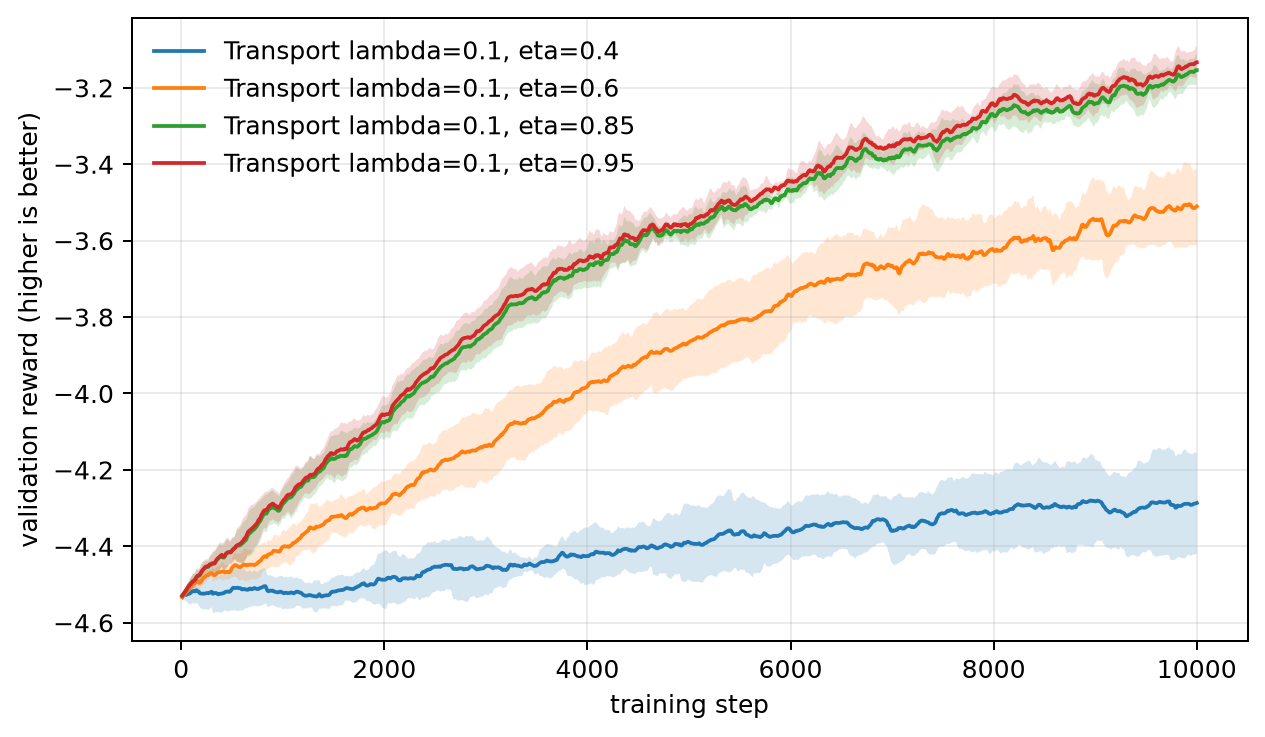
\includegraphics[width=0.49\linewidth]{figures/twostate_eta_sweep_T5.png}
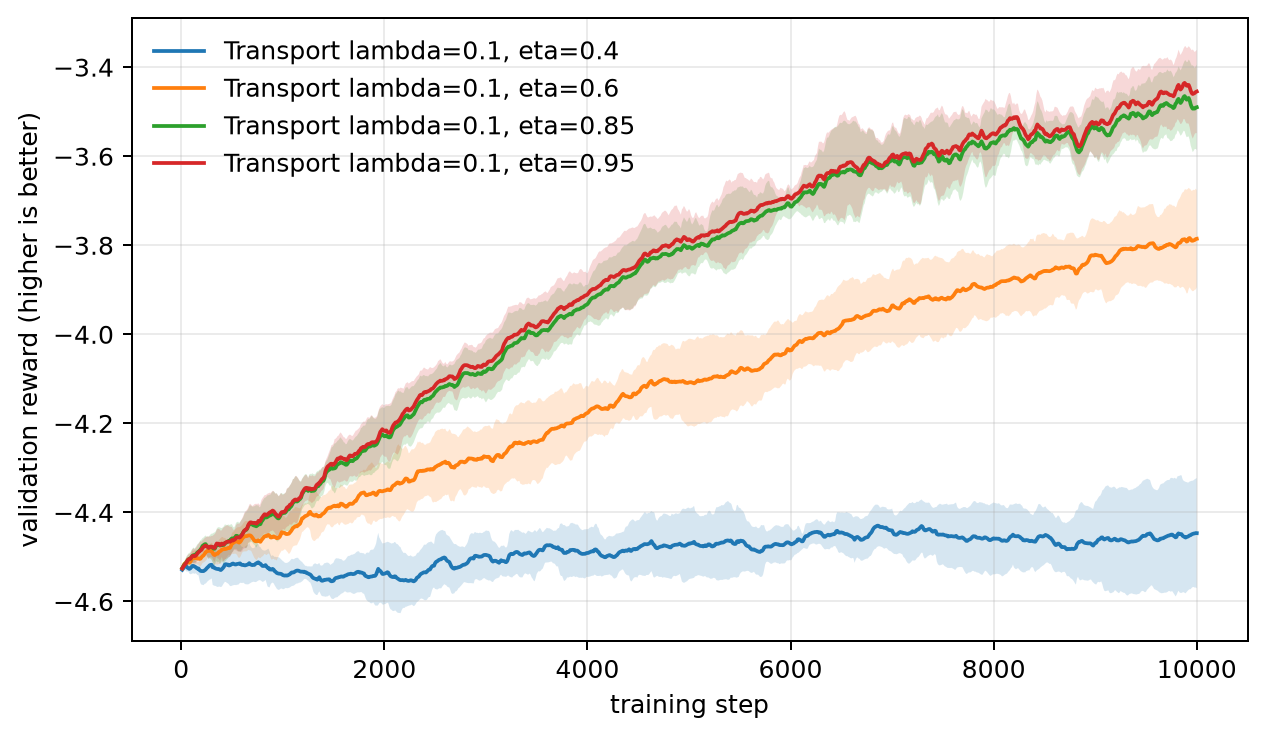
\includegraphics[width=0.49\linewidth]{figures/twostate_eta_sweep_T5_particle.png}
\caption{Two-state benchmark at $T=5$ and $\lambda=0.1$: effect of the auxiliary perturbation scale $\eta$ on the validation reward, as mean over five seeds with one standard deviation shaded, with exact population flow (left) and with a particle approximation of it (right). The ordering in $\eta$ is unchanged by the substitution; the particle runs are uniformly lower and noticeably noisier across seeds.}
\label{fig:twostate-eta}
\end{figure}

\begin{figure}[H]
\centering
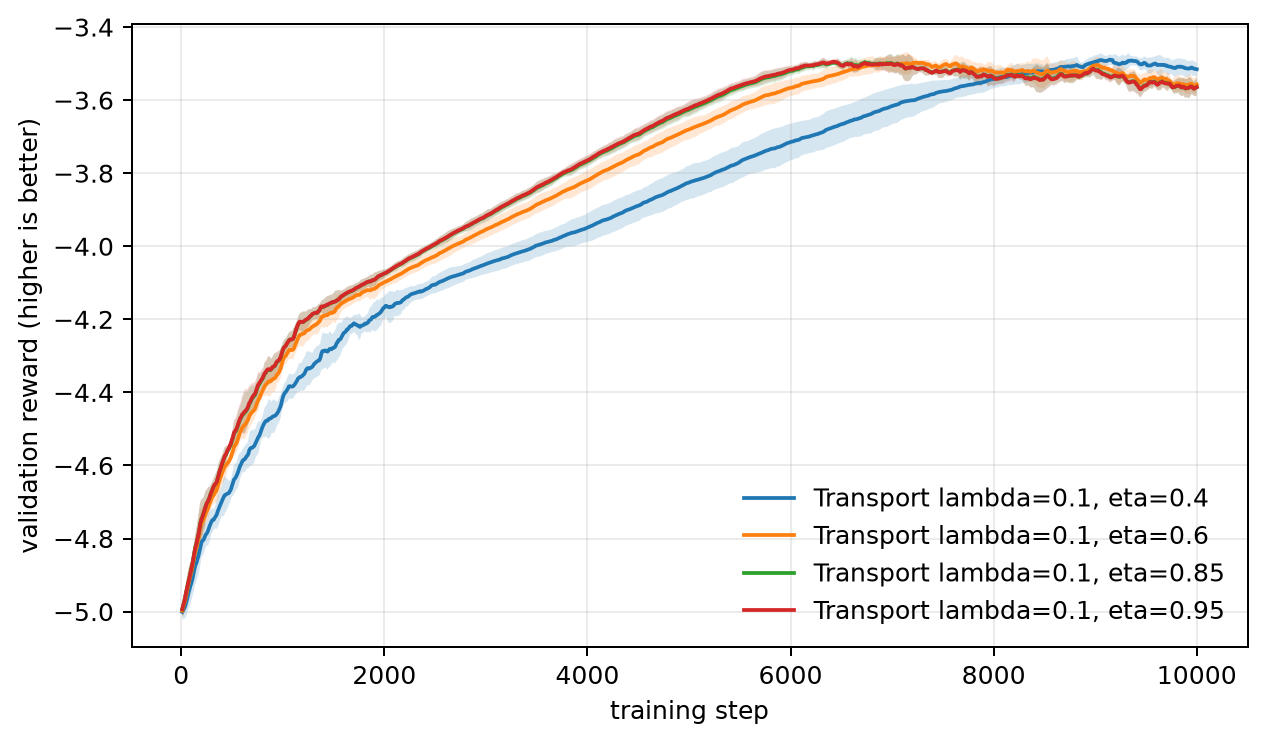
\includegraphics[width=0.49\linewidth]{figures/twostate_eta_sweep_T2.png}
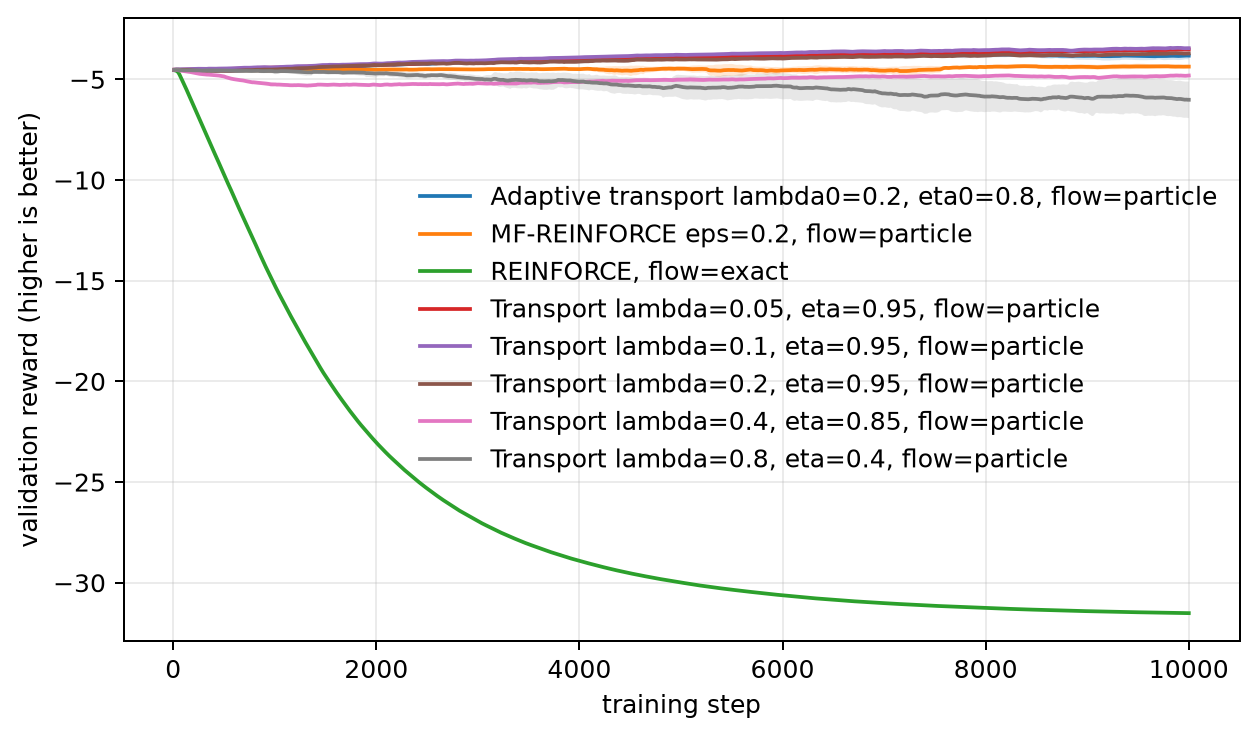
\includegraphics[width=0.49\linewidth]{figures/twostate_validation_T5_particle.png}
\caption{Two-state benchmark. Left: effect of the auxiliary scale $\eta$ at $T=2$ and $\lambda=0.1$, the shorter-horizon counterpart of Figure~\ref{fig:twostate-eta}. Right: validation reward at $T=5$ with a particle approximation of the population flow, to be compared with the exact-flow panel of Figure~\ref{fig:twostate-validation}.}
\label{fig:appendix-twostate}
\end{figure}

\section{Learned flows}
\begin{figure}[H]
\centering
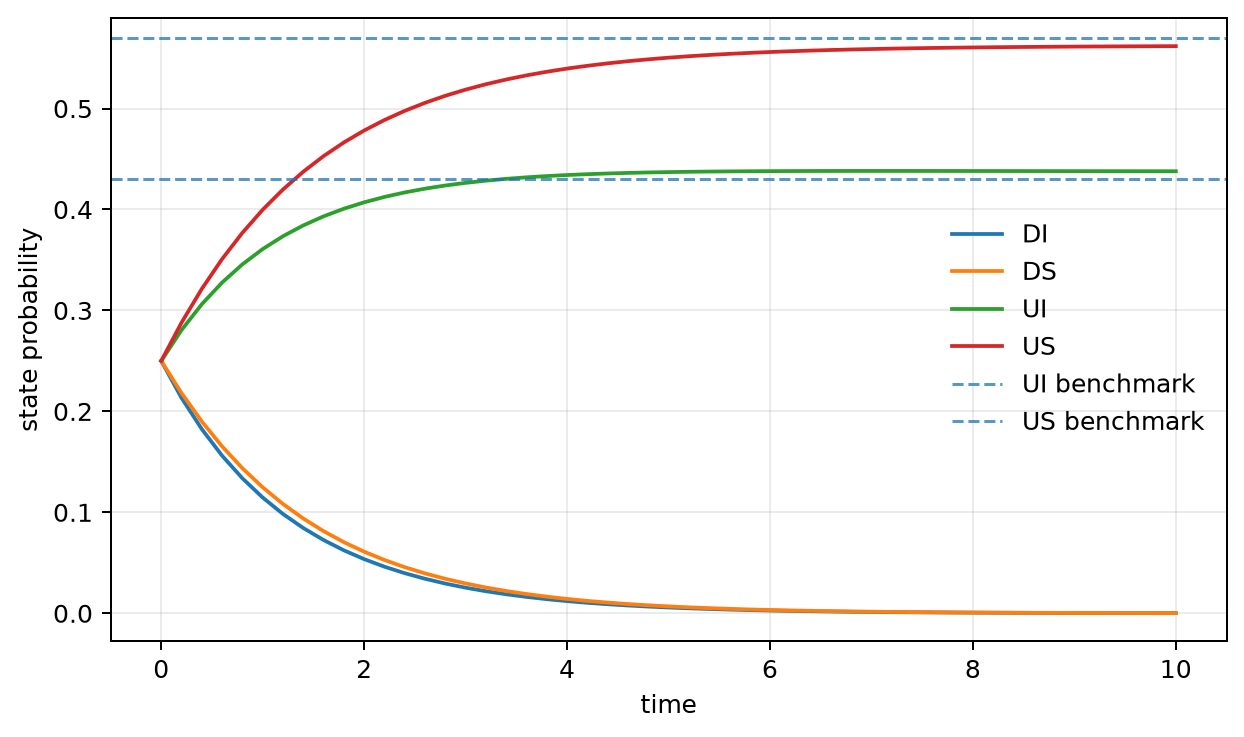
\includegraphics[width=0.49\linewidth]{figures/cyber_flow_reinforce.png}
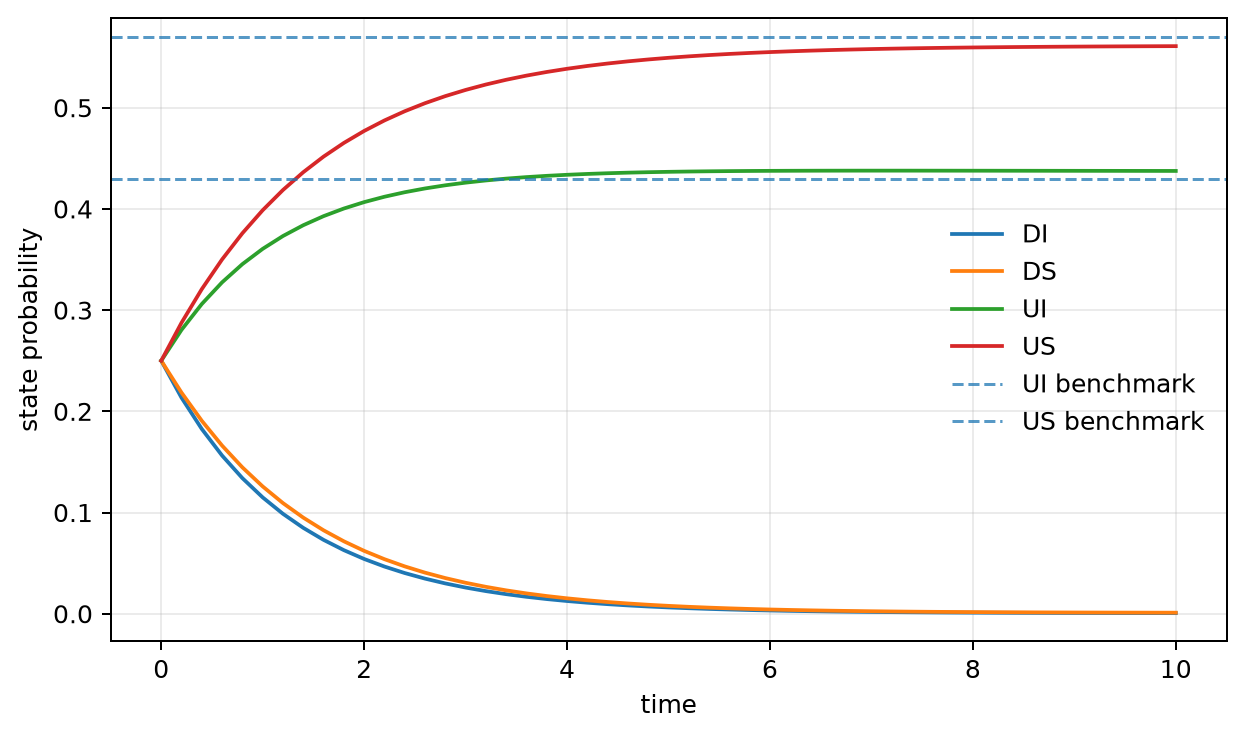
\includegraphics[width=0.49\linewidth]{figures/cyber_flow_mfreinforce.png}
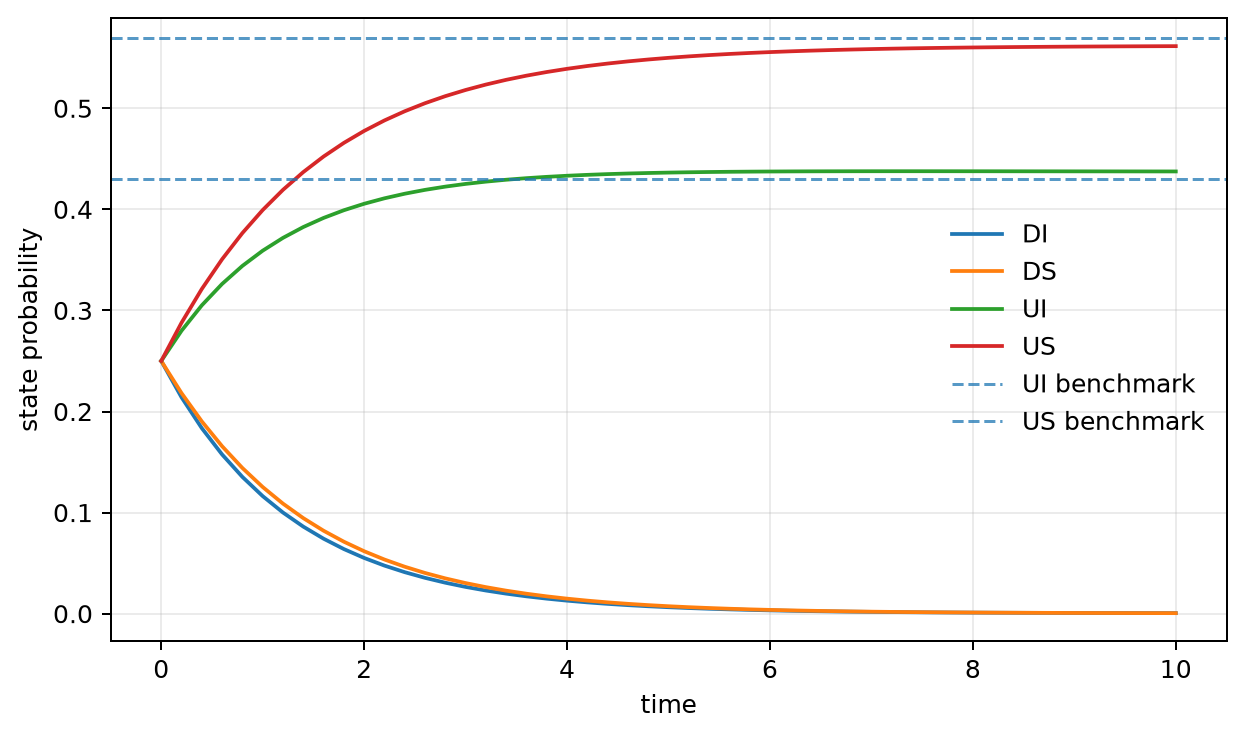
\includegraphics[width=0.49\linewidth]{figures/cyber_flow_transport.png}
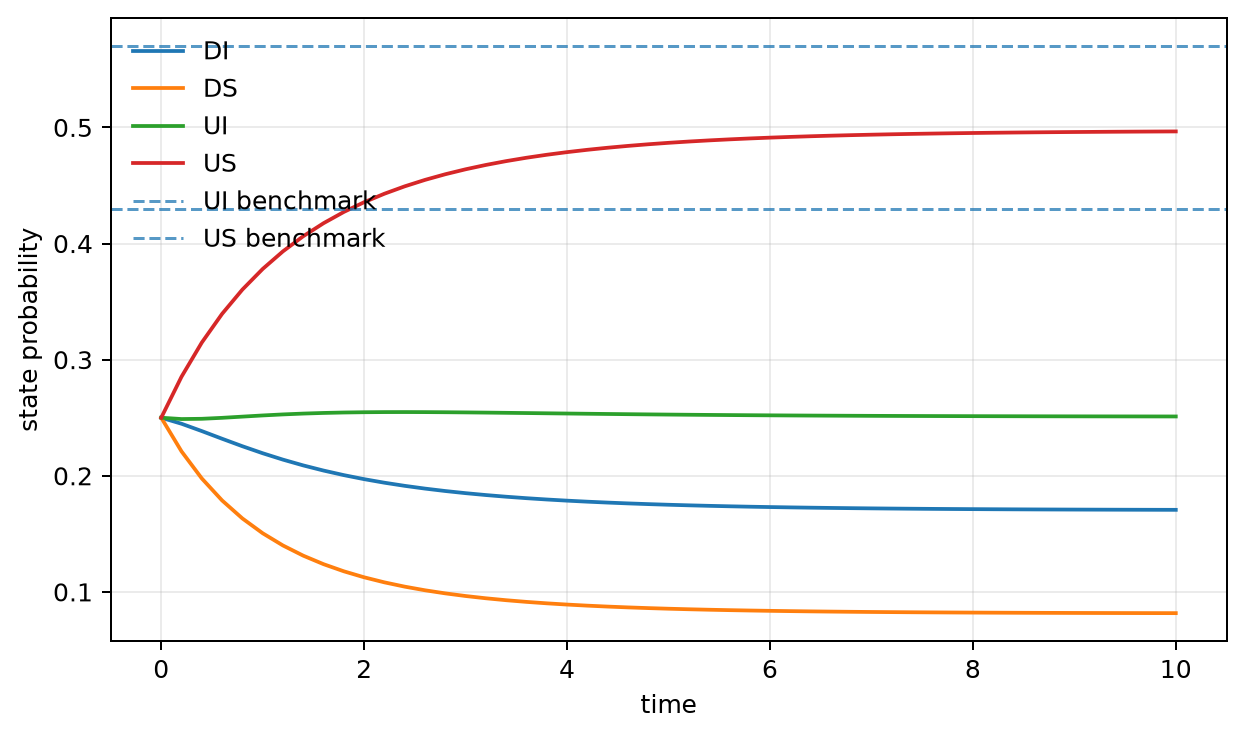
\includegraphics[width=0.49\linewidth]{figures/cyber_flow_adaptive.png}
\caption{Learned state distributions on the cybersecurity benchmark, propagated from the uniform validation law over the full validation episode of $T_{\mathrm{val}}=50$ steps. Top left: REINFORCE. Top right: MF-REINFORCE at $\varepsilon=1$. Bottom left: fixed-scale transport at $\lambda=0.4$. Bottom right: adaptive transport. The dashed lines mark the terminal probabilities of the undefended equilibrium. The first three estimators reach it; the adaptive controller keeps most of the population in the two defended states instead.}
\label{fig:cybersecurity-flows}
\end{figure}

\begin{figure}[H]
\centering
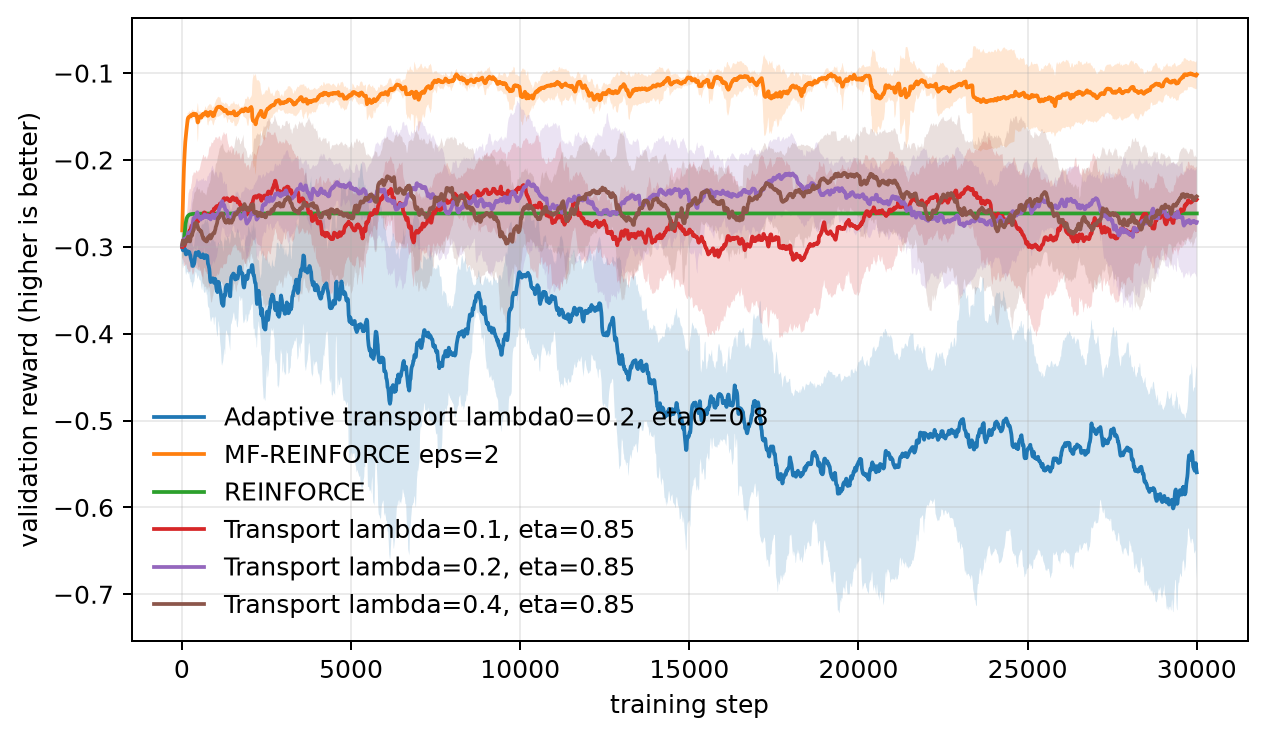
\includegraphics[width=0.62\linewidth]{figures/distribution_validation_T5.png}
\caption{Distribution-planning benchmark at $T=5$: validation reward against training iteration, as mean over five seeds with one standard deviation shaded. REINFORCE is the flat line at $-0.2616$; the transport curves oscillate over tens of thousands of iterations without settling.}
\label{fig:distribution-validation}
\end{figure}

\label{appendix:learned-flows}

Figure~\ref{fig:twostate-flows} compares the population flow learned by all four estimators on the two-state benchmark; the corresponding comparison on cybersecurity, Figure~\ref{fig:cybersecurity-flows}, is kept in the main text because it carries the explanation of that benchmark's ordering. Figure~\ref{fig:appendix-continuous-flows} gives the moment flows on the continuous-state benchmarks.

\begin{figure}[H]
\centering
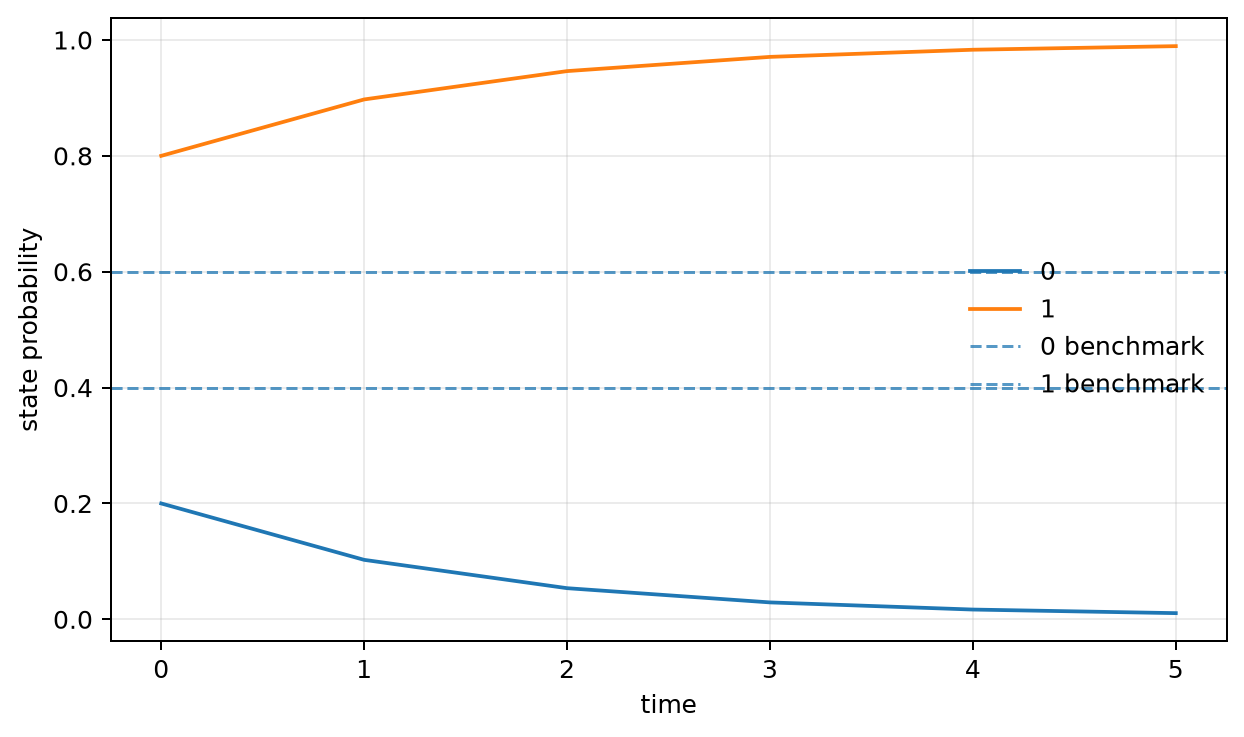
\includegraphics[width=0.49\linewidth]{figures/twostate_flow_reinforce.png}
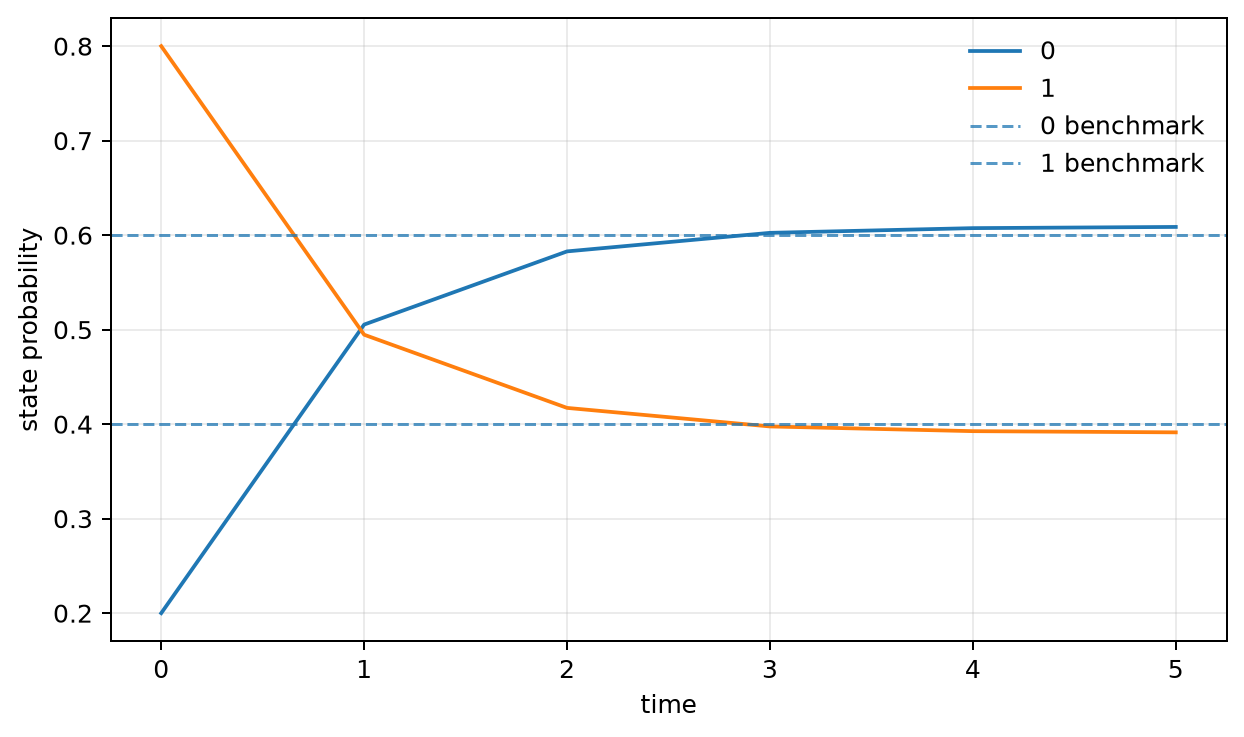
\includegraphics[width=0.49\linewidth]{figures/twostate_flow_mfreinforce.png}
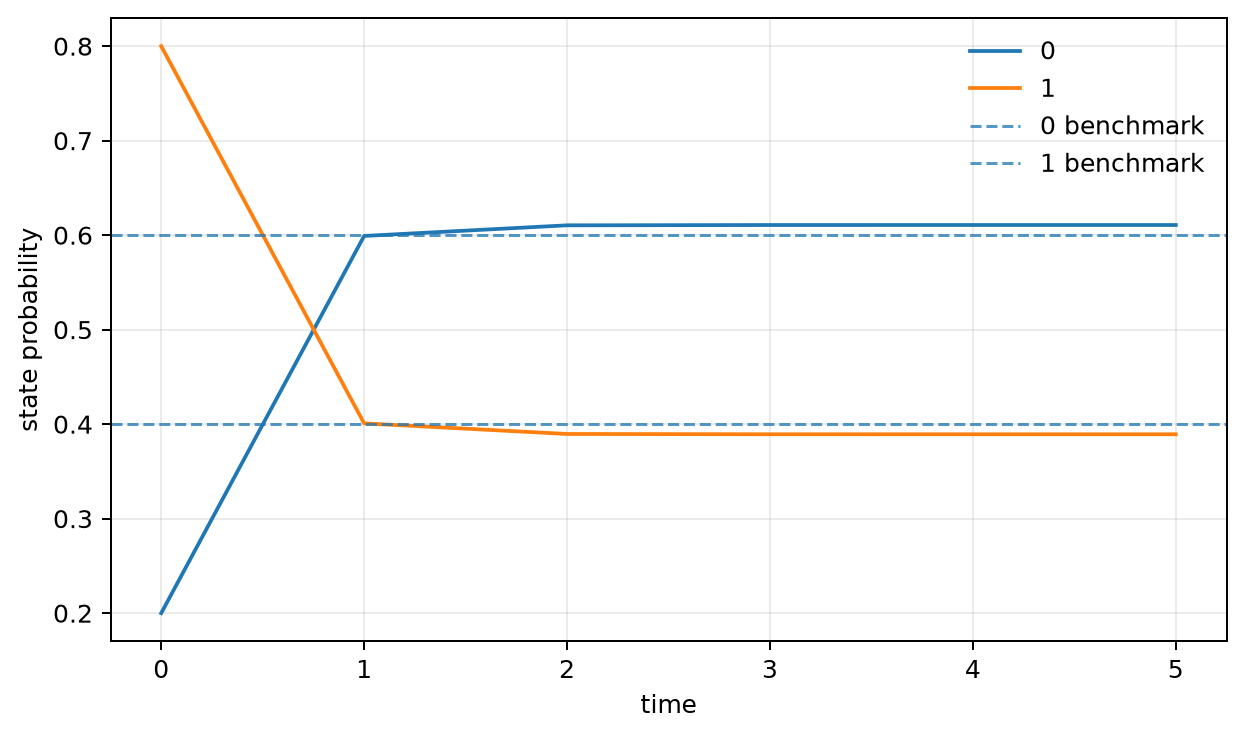
\includegraphics[width=0.49\linewidth]{figures/twostate_flow_transport.png}
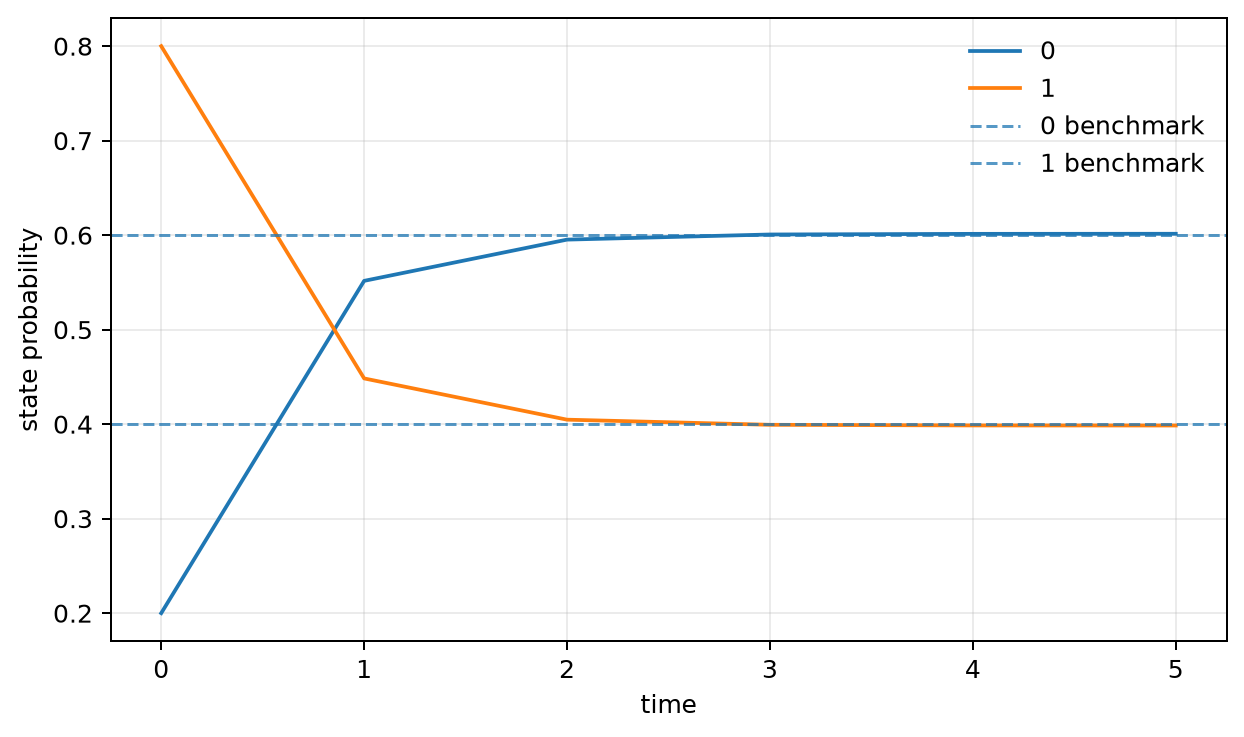
\includegraphics[width=0.49\linewidth]{figures/twostate_flow_adaptive.png}
\caption{Learned population flows on the two-state benchmark at $T=5$ with exact population flow, started from the validation law $\mu_0^{\mathrm{val}}=(0.2,0.8)$. Top left: REINFORCE. Top right: MF-REINFORCE at $\varepsilon=0.2$. Bottom left: fixed-scale transport at $\lambda=0.1$, $\eta=0.95$. Bottom right: adaptive transport. The dashed lines mark the target proportions $(0.6,0.4)$ that the closed-form optimal policy sustains.}
\label{fig:twostate-flows}
\end{figure}

The remaining validation curves follow.

\begin{figure}[H]
\centering
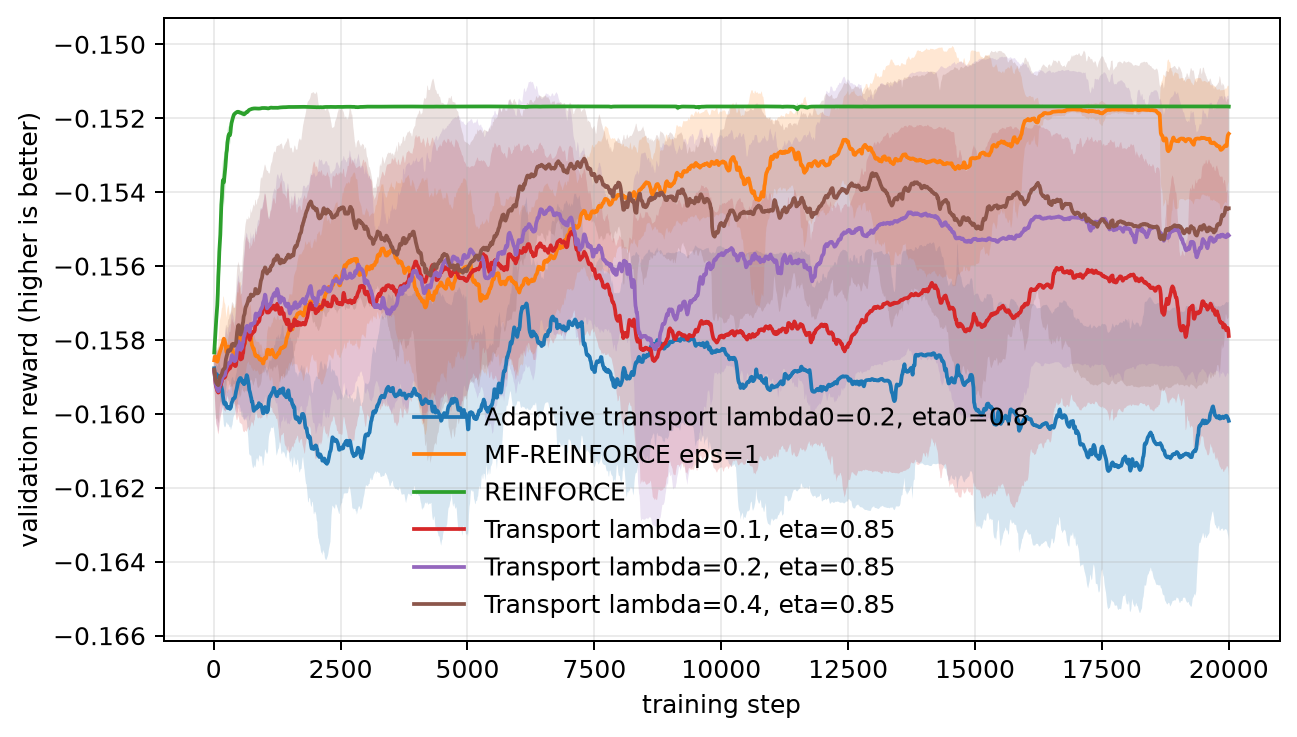
\includegraphics[width=0.68\linewidth]{figures/cybersecurity_validation_T3.png}
\caption{Cybersecurity benchmark at $T=3$: validation reward against training iteration, as mean over five seeds with one standard deviation shaded. REINFORCE converges within a few hundred iterations to the best value in the comparison, and the spread between the best and the worst estimator is under $6\%$ of the objective.}
\label{fig:cybersecurity-validation}
\end{figure}

\begin{figure}[H]
\centering
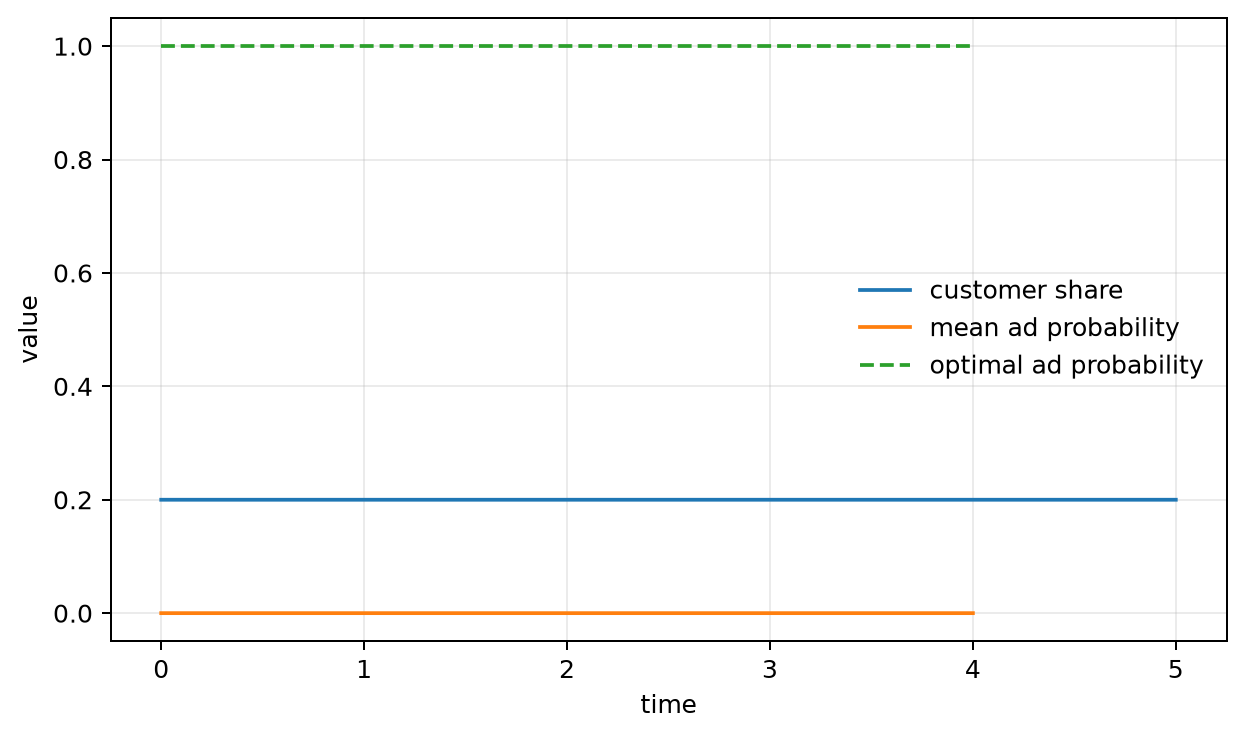
\includegraphics[width=0.32\linewidth]{figures/adv_reinforce.png}
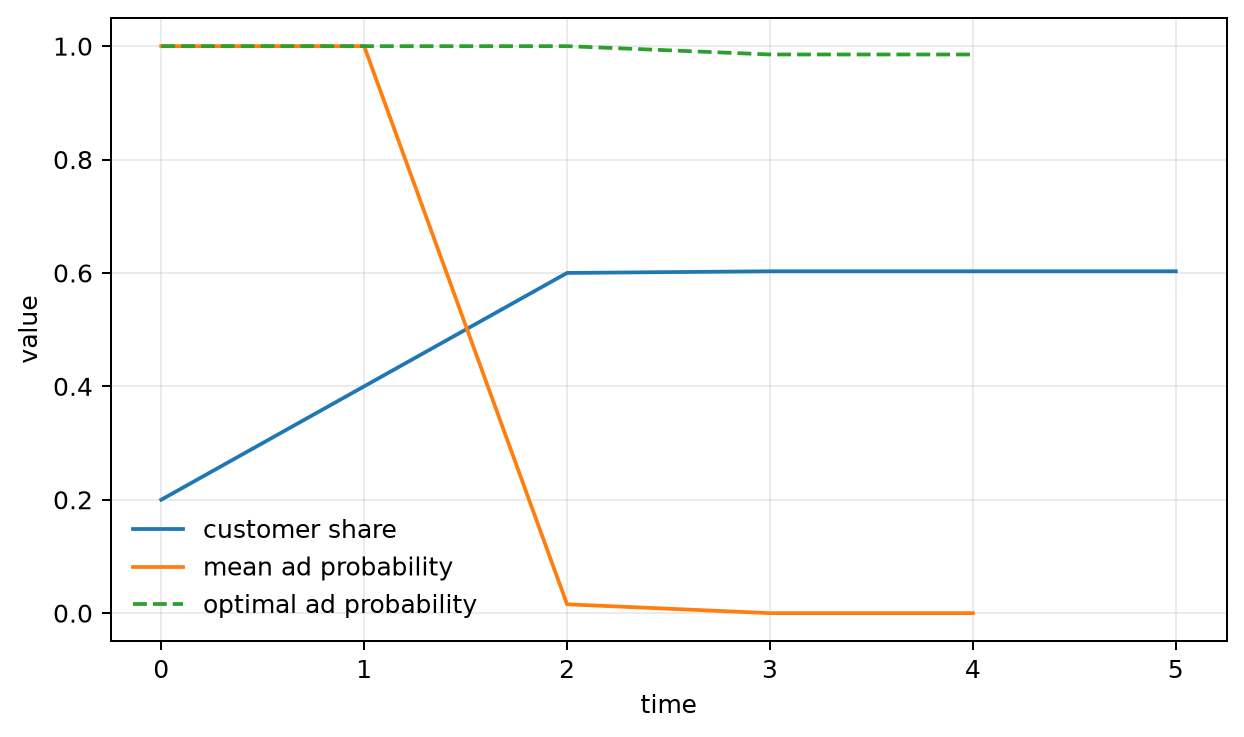
\includegraphics[width=0.32\linewidth]{figures/adv_mfreinforce.png}
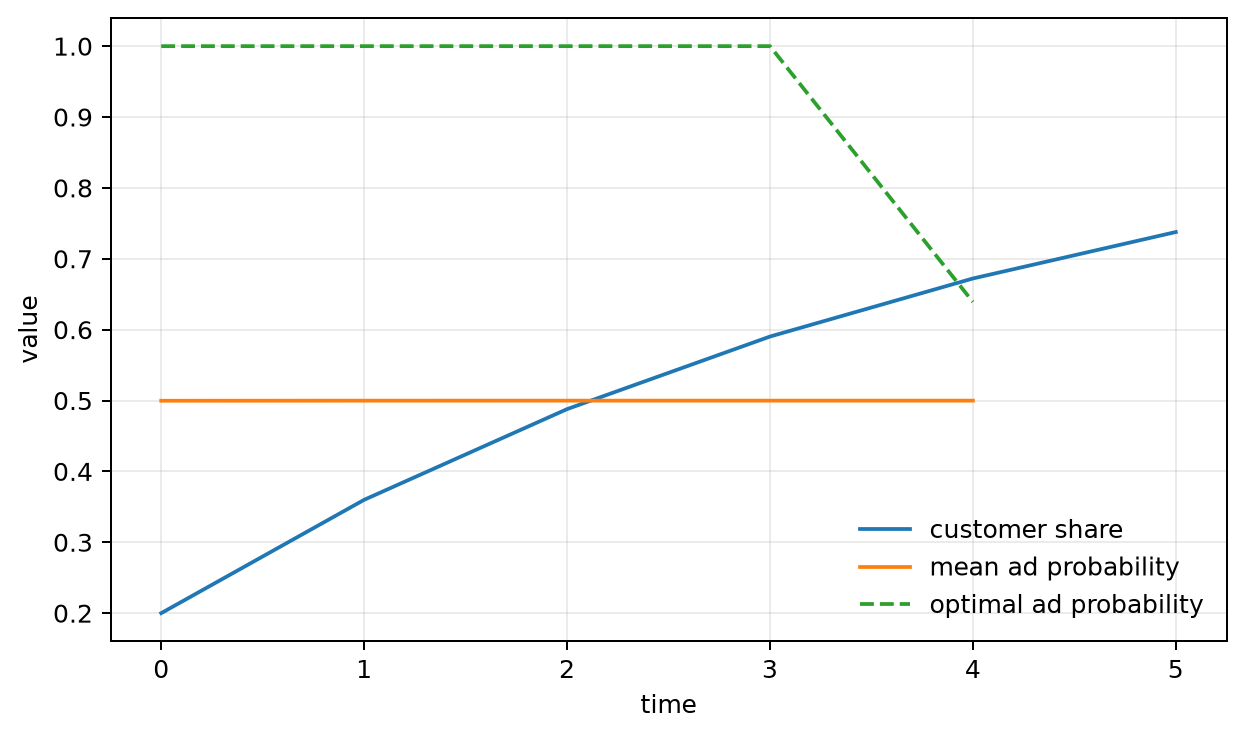
\includegraphics[width=0.32\linewidth]{figures/adv_transport.png}
\caption{Targeted-advertising benchmark at $T=5$: customer share and population-averaged advertising probability of the learned policy against the reference $\widehat q$, for REINFORCE (left), MF-REINFORCE at $\varepsilon=1$ (centre) and fixed-scale transport at $\lambda=0.1$ (right), on the best seed of each. The averaged advertising probability hides a structural difference between the last two, which Table~\ref{tab:advertising-policies} resolves.}
\label{fig:advertising-policy-panels}
\end{figure}

\begin{figure}[H]
\centering
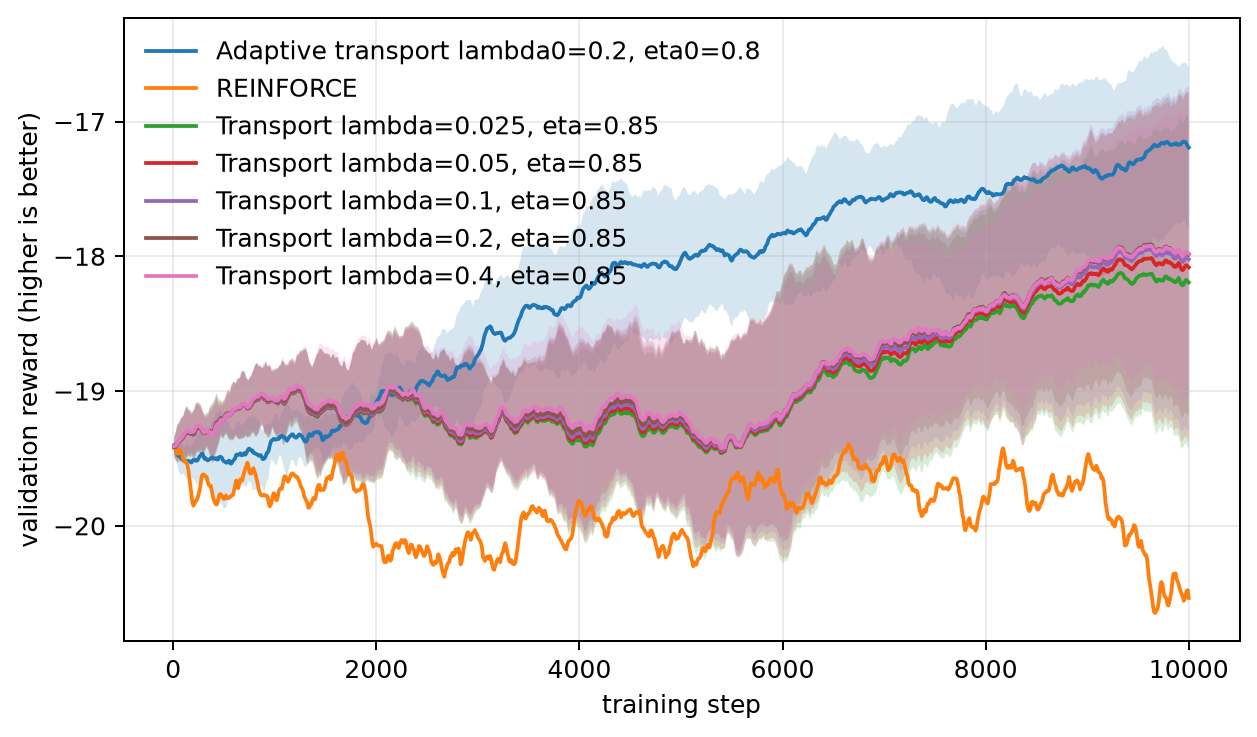
\includegraphics[width=0.68\linewidth]{figures/portfolio_validation_T10.png}
\caption{Mean--variance portfolio benchmark at $T=10$: validation reward against training iteration, as mean over five seeds with one standard deviation shaded. REINFORCE degrades below its initialization; the transport variants improve throughout, and the adaptive controller improves fastest.}
\label{fig:portfolio-validation}
\end{figure}

The figure below gives the moment flows on the continuous-state benchmarks. These are qualitative checks rather than measurements: they verify that the learned policies produce coherent population trajectories rather than the oscillation or collapse that a badly scaled sensitivity estimate would cause.

\begin{figure}[H]
\centering
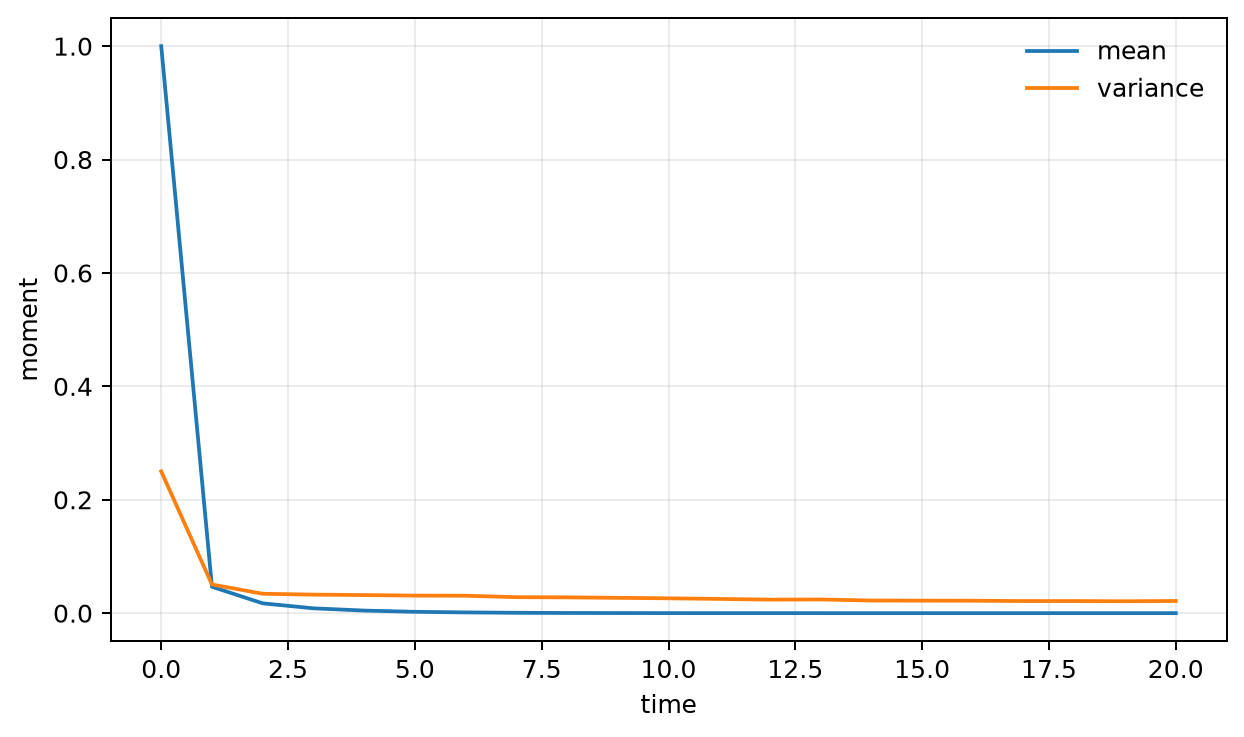
\includegraphics[width=0.46\linewidth]{figures/lq_moment_flow.png}
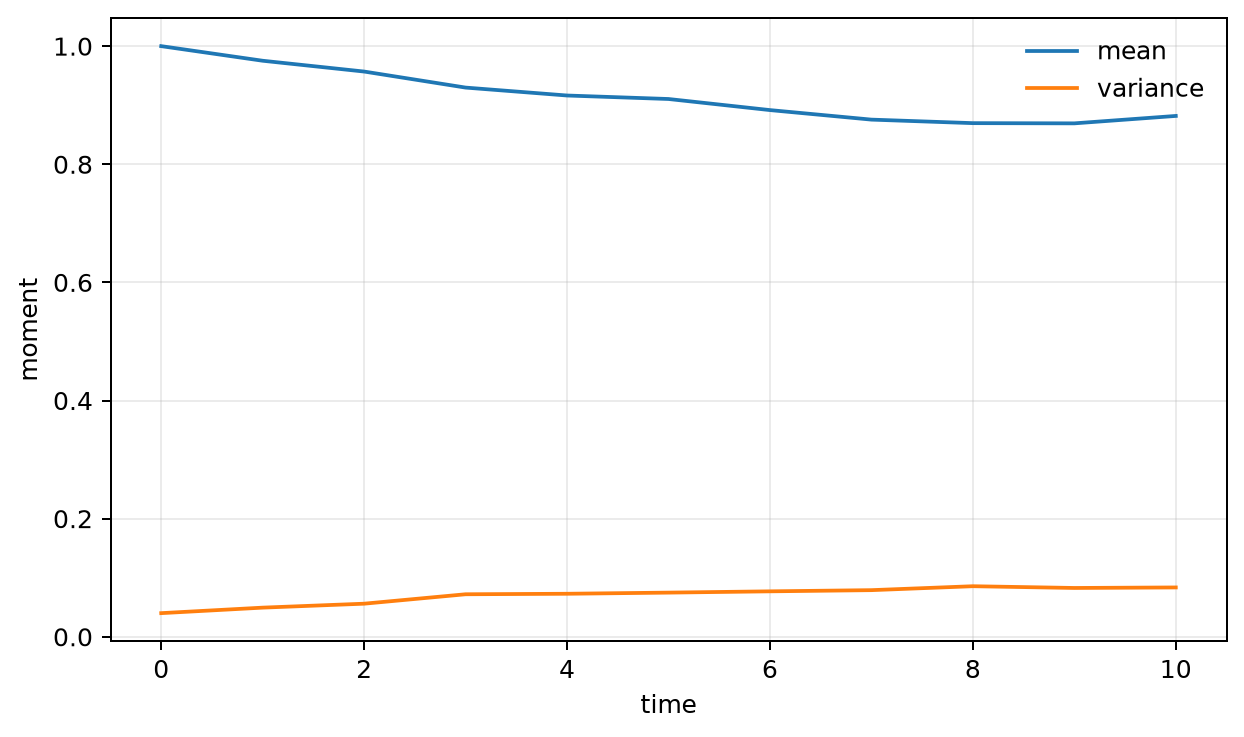
\includegraphics[width=0.46\linewidth]{figures/portfolio_moment_flow.png}
\caption{Learned moment flows on the continuous-state benchmarks, for the best fixed-scale transport configuration of each: linear--quadratic at $T=20$ and $\lambda=0.1$ (left) and portfolio at $T=10$ and $\lambda=0.4$ (right).}
\label{fig:appendix-continuous-flows}
\end{figure}

\section{Population-flow approximation}
\label{appendix:flow-comparison}

\begin{figure}[H]
\centering
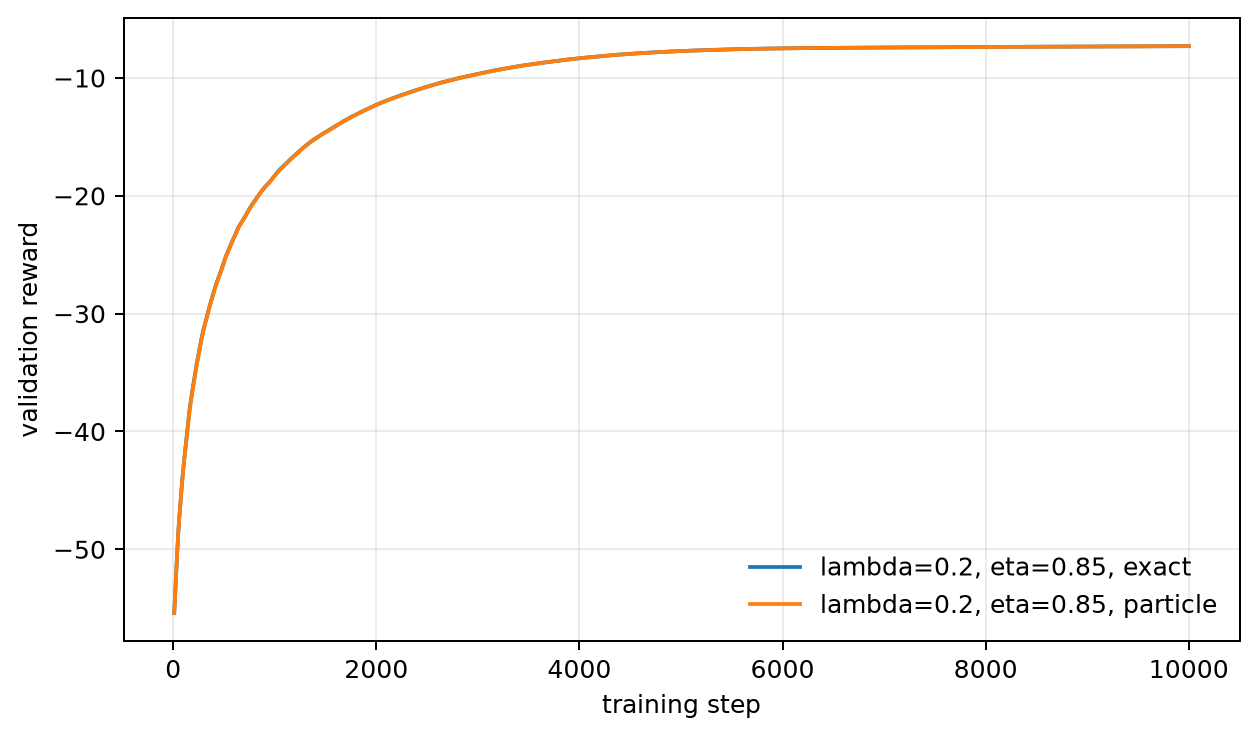
\includegraphics[width=0.62\linewidth]{figures/lq_flow_comparison.png}
\caption{Linear--quadratic benchmark at $T=20$ and $\lambda=0.2$: exact moment recursion against particle estimation of the population flow, as mean over five seeds. The two curves coincide to within the line width.}
\label{fig:lq-flow-comparison}
\end{figure}

Figure~\ref{fig:lq-flow-comparison} compares exact and particle population flow on the linear--quadratic benchmark at $\lambda=0.2$, and Figure~\ref{fig:appendix-flow-comparison} repeats the comparison at the two ends of the perturbation grid. The two flow modes remain indistinguishable at every scale, which is the expected behaviour when the population law enters the dynamics only through its mean.

\begin{figure}[H]
\centering
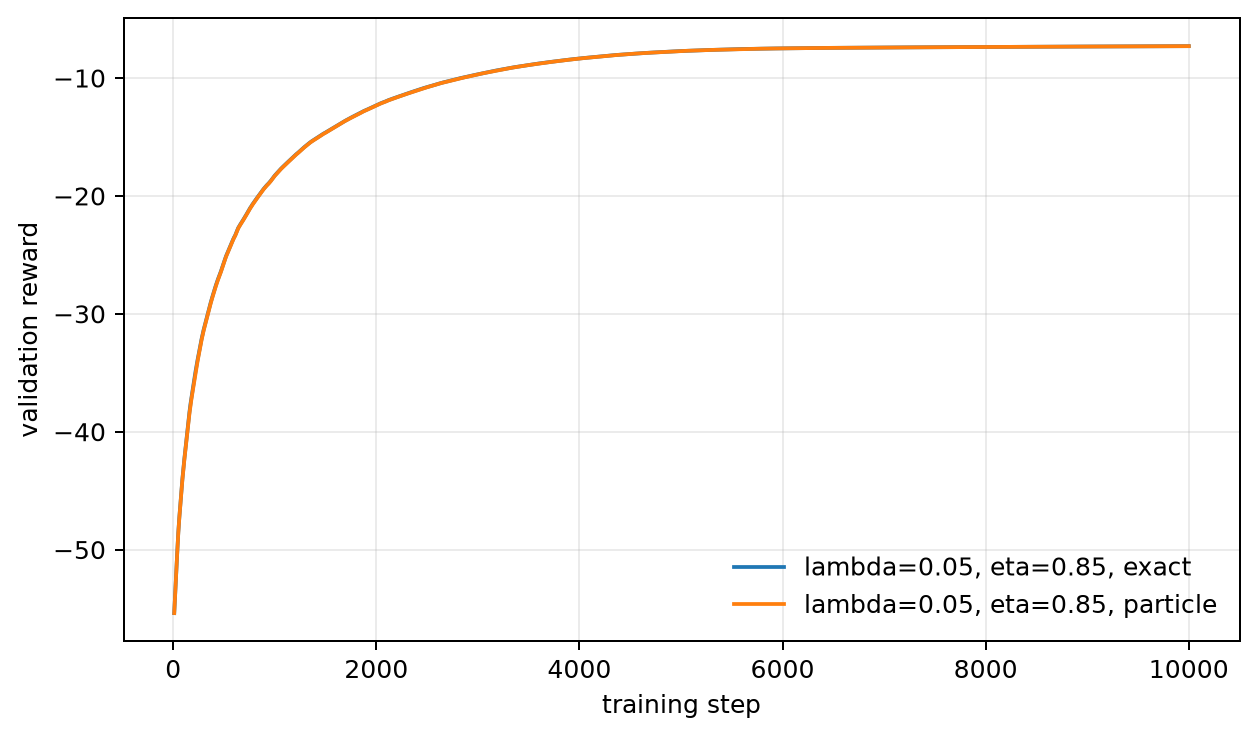
\includegraphics[width=0.49\linewidth]{figures/lq_flow_comparison_l005.png}
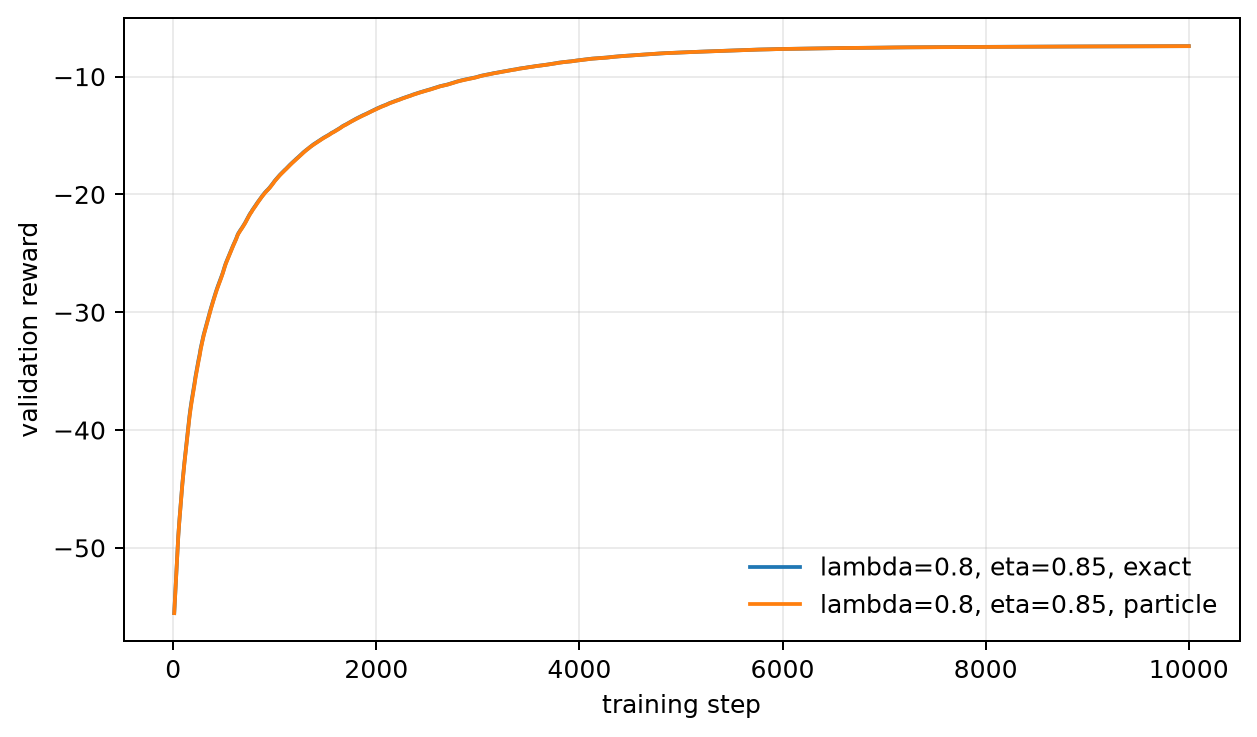
\includegraphics[width=0.49\linewidth]{figures/lq_flow_comparison_l08.png}
\caption{Linear--quadratic benchmark at $T=20$: exact against particle population flow at $\lambda=0.05$ (left) and $\lambda=0.8$ (right), as mean over five seeds.}
\label{fig:appendix-flow-comparison}
\end{figure}

\section{Adaptive schedules}
\label{appendix:adaptive-schedules}

\begin{figure}[H]
\centering
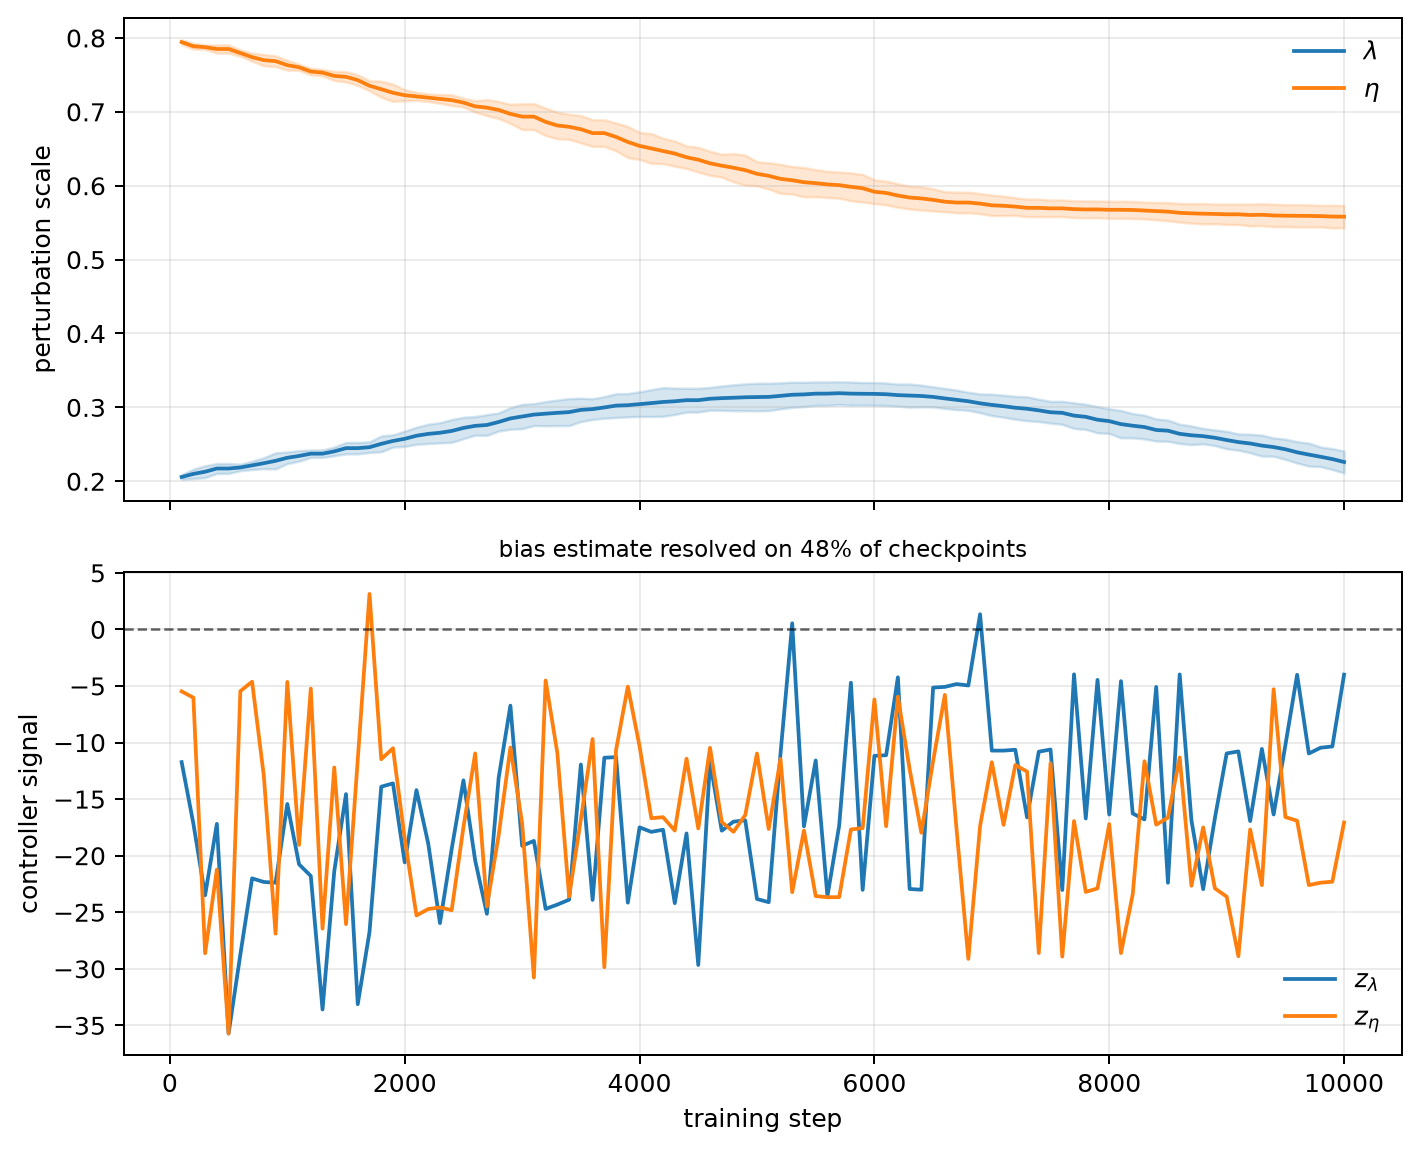
\includegraphics[width=0.62\linewidth]{figures/lq_adaptive_schedule.png}
\caption{Adaptive controller on the linear--quadratic benchmark at $T=20$ with exact population flow. Top: perturbation scales against training iteration, as mean over five seeds with one standard deviation shaded. Bottom: the logarithmic balance signals $z_\lambda$ and $z_\eta$, negative almost everywhere, indicating a variance-dominated regime.}
\label{fig:adaptive-schedule}
\end{figure}

Figure~\ref{fig:adaptive-schedule} shows the controller trajectory on the linear--quadratic benchmark. Figure~\ref{fig:appendix-adaptive} gives the two benchmarks on which the controller underperforms the fixed grid. Both contract the main scale to the bottom of its range, and the contrast with the linear--quadratic trajectory, which is non-monotone in $\lambda$ and settles an order of magnitude higher, is the observation discussed in Section~\ref{sec:adaptive-control}.

\begin{figure}[H]
\centering
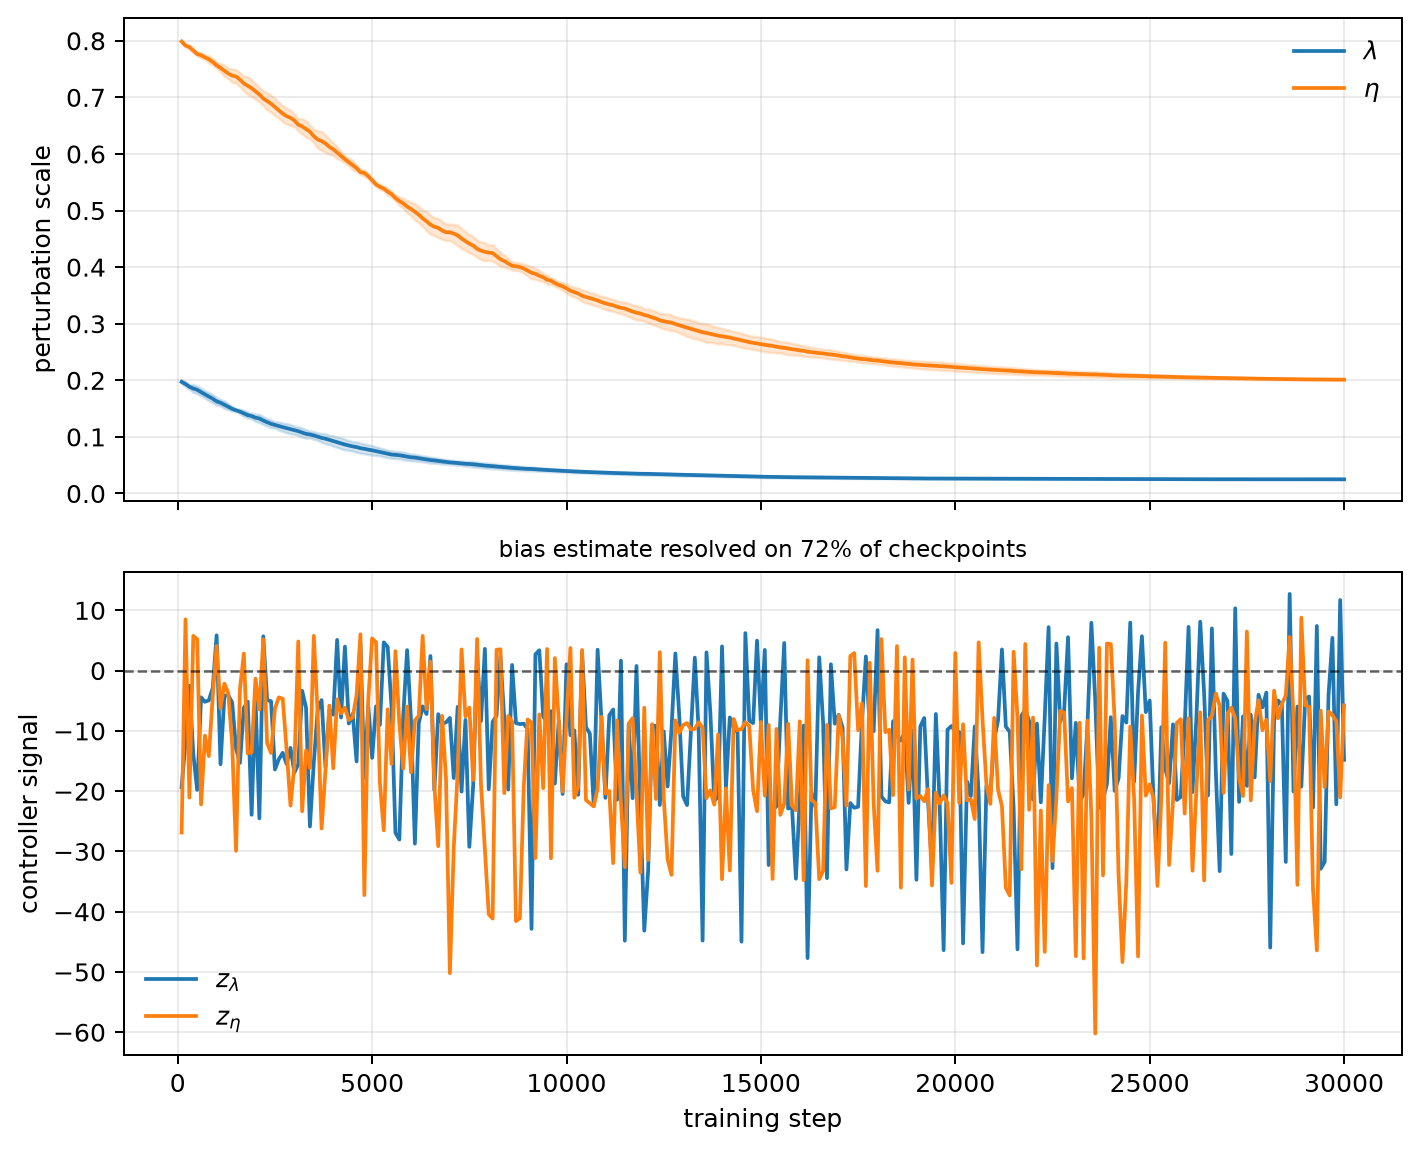
\includegraphics[width=0.49\linewidth]{figures/distribution_adaptive_schedule.png}
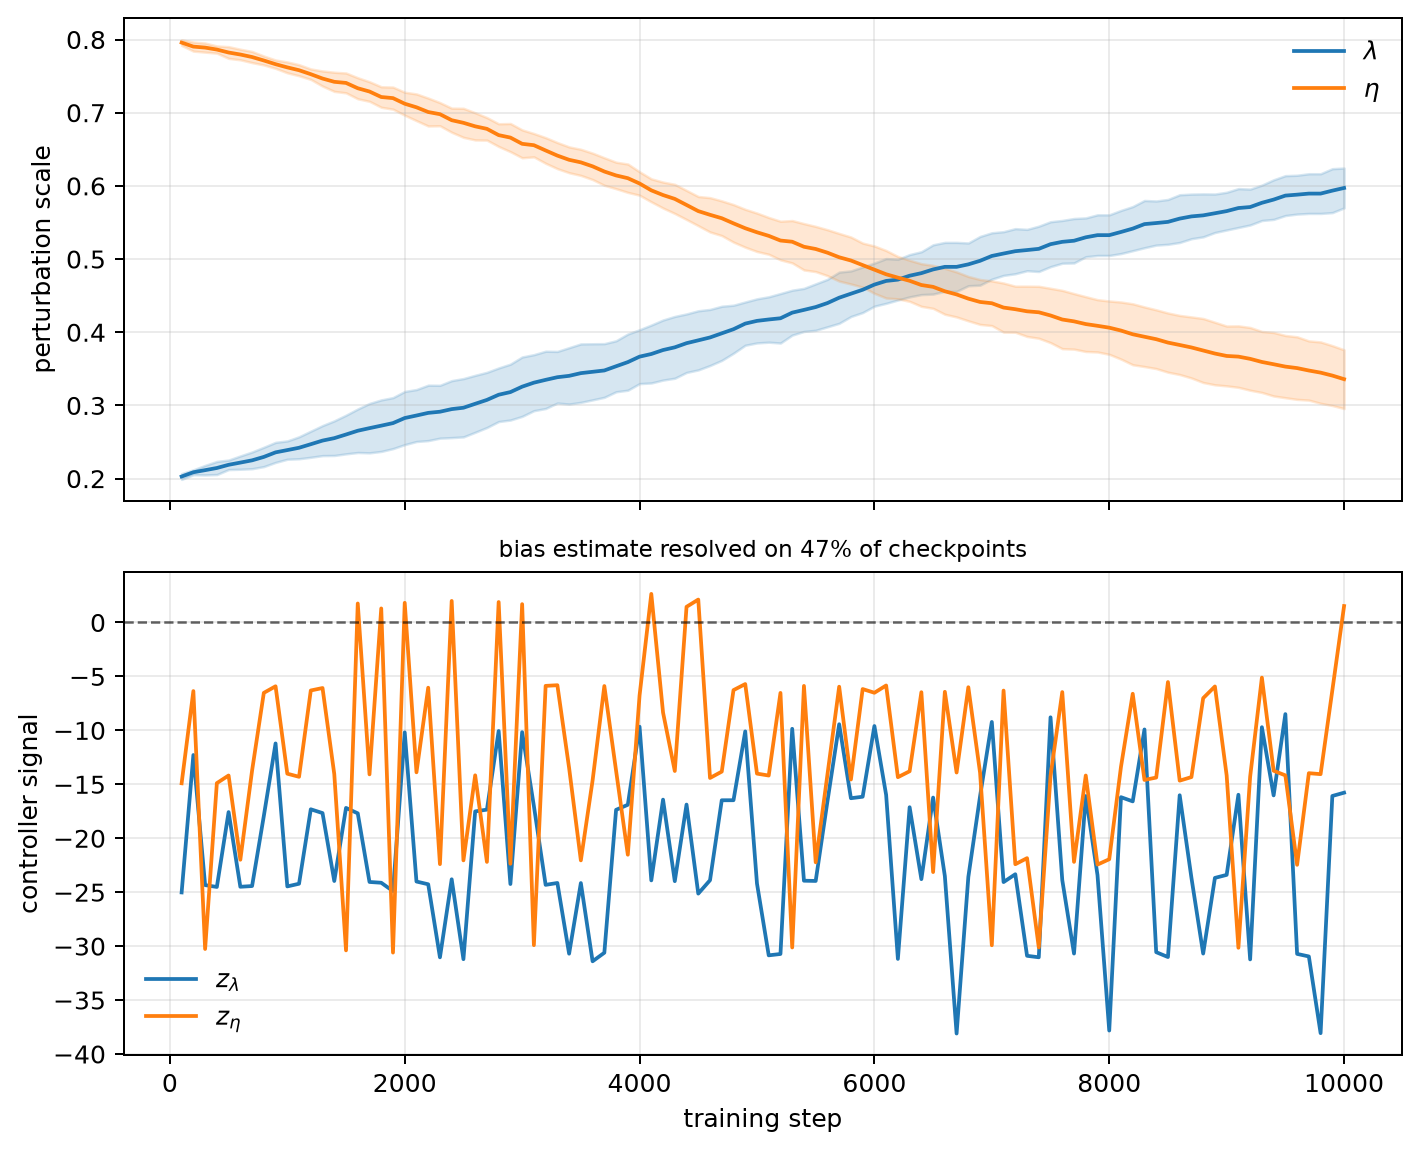
\includegraphics[width=0.49\linewidth]{figures/portfolio_adaptive_schedule.png}
\caption{Adaptive controller on distribution planning at $T=5$ (left) and on the portfolio benchmark at $T=10$ (right). Top panels: perturbation scales against training iteration, as mean over five seeds with one standard deviation shaded. Bottom panels: the logarithmic balance signals $z_\lambda$ and $z_\eta$.}
\label{fig:appendix-adaptive}
\end{figure}

\section{Allocating the auxiliary budget}
\label{appendix:auxiliary-budget}

The equal-budget rule of Section~\ref{subsec:experimentation-protocol} fixes the total number of simulated transitions per update, $T(B_{\mathrm{tr}}+n_{\mathrm{tr}})$, but not its split between the main trajectories and the auxiliary sensitivity estimate. Table~\ref{tab:auxiliary-budget} records that split on every benchmark, together with the number $d$ of free coordinates of the population argument that the auxiliary estimate has to resolve.

\begin{table}[H]
\centering
\begin{tabular}{llrrrrr}
\toprule
Benchmark & Argument & $d$ & $B_{\mathrm{tr}}$ & $n_{\mathrm{tr}}$ & $n_{\mathrm{tr}}/d$ & Budget \\
\midrule
Two-state & $\Delta_2$ & 1 & 248 & 12 & $12.0$ & $1\,300$ \\
Cybersecurity & $\Delta_4$ & 3 & 184 & 20 & $6.7$ & $612$ \\
Distribution planning & $\Delta_{10}$ & 9 & 549 & 11 & $1.2$ & $2\,800$ \\
Targeted advertising & $\Delta_2$ & 1 & 248 & 12 & $12.0$ & $1\,300$ \\
Linear--quadratic & mean & 1 & 201 & 20 & $20.0$ & $4\,420$ \\
Portfolio & mean & 1 & 311 & 200 & $200.0$ & $5\,110$ \\
\bottomrule
\end{tabular}
\caption{Split of the matched simulator budget between the main trajectories $B_{\mathrm{tr}}$ and the auxiliary sensitivity trajectories $n_{\mathrm{tr}}$ of the fixed-scale transport estimator, with $d$ the number of free coordinates of the population argument. The equal-budget rule constrains $T(B_{\mathrm{tr}}+n_{\mathrm{tr}})$ but not the split, which was reallocated towards the auxiliary estimate on the continuous-state benchmarks and left at the default on the finite-state ones. The resulting auxiliary sample size per coordinate spans more than two orders of magnitude, and distribution planning is the one benchmark where it falls close to one.}
\label{tab:auxiliary-budget}
\end{table}


The ratio $n_{\mathrm{tr}}/d$ spans more than two orders of magnitude across the suite, and distribution planning is the extreme case. Its transport runs use $B_{\mathrm{tr}}=549$ main and $n_{\mathrm{tr}}=11$ auxiliary trajectories against a ten-point simplex with $d=9$, that is $1.2$ auxiliary trajectories per coordinate, against $6.7$ on cybersecurity, $12$ on the two-state and advertising problems, $20$ on the linear--quadratic benchmark and $200$ on the portfolio benchmark. It is the only benchmark on which the auxiliary estimate is asked to resolve more coordinates than it has samples, and the only finite-state benchmark on which transport loses to MF-REINFORCE by a wide margin. Whether that association is causal is the question taken up as an extension in Section~\ref{sec:extensions}. This section records the two measurements bearing on it: what a reallocation costs, and what it does on a benchmark where the hypothesis predicts nothing.

\paragraph{The cost of reallocating.}
The split can be changed without changing the budget, since the rule constrains only the sum: on distribution planning, taking $B_{\mathrm{tr}}=200$ and $n_{\mathrm{tr}}=360$ leaves $T(B_{\mathrm{tr}}+n_{\mathrm{tr}})=2\,800$ unchanged and raises the auxiliary sample size to $40$ per coordinate. It is also affordable in arithmetic. One might expect the cost of the update to grow linearly in $n_{\mathrm{tr}}$, but the sensitivity recursion is applied to the whole auxiliary batch at once, and a direct measurement gives a factor $1.9$ in seconds per training step when $n_{\mathrm{tr}}$ goes from $11$ to $360$, a $33$-fold increase in auxiliary samples. The dominant cost of the update on this benchmark is the exact population recursion over the ten-point simplex, which the reallocation does not touch. Applied to a base cost of $6\,802$ seconds per transport seed over $30\,000$ iterations (Table~\ref{tab:budget-runtime}), that factor nonetheless puts a five-seed reallocated arm outside the compute budget of the internship so far, which is why the experiment is proposed in Section~\ref{sec:extensions} rather than reported here.

\paragraph{A negative control on targeted advertising.}
Table~\ref{tab:reallocation} reports the same reallocation on a benchmark where the hypothesis predicts no effect. The advertising population argument is a two-point simplex with a single free coordinate, and its transport runs already use $n_{\mathrm{tr}}=12$ auxiliary trajectories, the same ratio as the two-state benchmark on which transport is the best estimator at $T=5$. Moving the split from $(B_{\mathrm{tr}},n_{\mathrm{tr}})=(248,12)$ to $(100,160)$ at fixed budget takes the final objective from $0.9795\pm0.0089$ to $0.9734\pm0.0079$, a difference well inside one standard deviation. Where the auxiliary estimate is already resolved, moving budget towards it does not help, which is what the hypothesis predicts; Section~\ref{subsec:targeted-advertising} identifies a different mechanism as the limitation there. The control establishes the absence of an effect where the ratio is already high; the positive arm is what the extension of Section~\ref{sec:extensions} would supply.

\begin{table}[H]
\centering
\small
\begin{tabular}{llrrrrrr}
\toprule
Benchmark & $\lambda$ & $B_{\mathrm{tr}}$ & $n_{\mathrm{tr}}$ & $n_{\mathrm{tr}}/d$ & Iterations & Objective & Seeds \\
\midrule
Targeted advertising & $0.1$ & 248 & 12 & $12.0$ & $10\,000$ & $0.9795\pm0.0089$ & 5 \\
 &  & 100 & 160 & $160.0$ &  & $0.9734\pm0.0079$ & 5 \\
\bottomrule
\end{tabular}
\caption{Recorded check of moving the matched simulator budget from the main trajectories towards the auxiliary sensitivity estimate. Both rows use the same estimator, perturbation scales, simulator budget $T(B_{\mathrm{tr}}+n_{\mathrm{tr}})$ and number of training iterations; only the split differs. The table compares the two allocations at the iteration count given in the sixth column, reading the default arm from its recorded validation history at the same point, and reports the mean and standard deviation over the seeds indicated. Higher is better.}
\label{tab:reallocation}
\end{table}


\section{Perturbation bound along the learned flows}
\label{appendix:theory-tables}
\label{appendix:tv-bounds}

Table~\ref{tab:tv-bounds} is the first of the measurement tables behind Table~\ref{tab:theory-verdicts} of Section~\ref{sec:theory-validation}, recording the largest value of $d_{\mathrm{TV}}(M_t^{\lambda,\theta},\mu_t^\theta)/\lambda$ along the learned flow of every finite-state transport run. The other two, the objective bias against the perturbation scale and the replicated gradient diagnostics, are reported in the body of that section.

\begin{table}[H]
\centering
\begin{tabular}{lrrrr}
\toprule
Benchmark & Configurations & Measured points & $\max_t d_{\mathrm{TV}}/\lambda$ & Satisfies $d_{\mathrm{TV}}\leq\lambda$ \\
\midrule
Two-state & 80 & 400 & $0.800$ & 400/400 \\
Cybersecurity & 3 & 15 & $0.843$ & 15/15 \\
Distribution planning & 3 & 15 & $1.000$ & 15/15 \\
Targeted advertising & 3 & 15 & $0.800$ & 15/15 \\
\midrule
Total & $89$ & $445$ & & 445/445 \\
\bottomrule
\end{tabular}
\caption{Perturbation bound on the finite-state benchmarks. For every transport run the largest value of $d_{\mathrm{TV}}(M_t^{\lambda,\theta},\mu_t^\theta)$ along the learned population flow is compared with $\lambda$. The bound holds at every measured point, and is attained to within a factor $d_{\mathrm{TV}}(q_t,\mu_t^\theta)\leq1$ of $\lambda$, so the perturbation is neither degenerate nor larger than the theory allows.}
\label{tab:tv-bounds}
\end{table}


\section{The population-dependence ablation}
\label{appendix:gamma-ablation}

Table~\ref{tab:correction-alignment-ablation} is the controlled pair discussed in Section~\ref{sec:correction-alignment}.

\begin{table}[H]
\centering
\begin{tabular}{llrrrl}
\toprule
Benchmark & Setting & $\|G_{\mathrm{full}}\|$ & $\|G_{\mathrm{det}}\|$ & $\varrho$ & Observed ordering \\
\midrule
Portfolio & $\gamma=0$   & 0.083 & 0.083 & $+1.000\pm0.000$ & REINFORCE $>$ transport \\
Portfolio & $\gamma=2$   & 1.357 & 0.083 & $-0.196\pm0.007$ & transport $>$ REINFORCE \\
\bottomrule
\end{tabular}
\caption{Switching the explicit population dependence on reverses the sign of $\varrho$ with the dynamics held fixed, and the ordering of the estimators reverses with it. At $\gamma=0$ the terminal reward depends on the population only through the centred variable $x-\mu$, the correction vanishes identically, and REINFORCE is exact; at $\gamma=2$ the correction is large and weakly aligned, and the transport estimator wins.}
\label{tab:correction-alignment-ablation}
\end{table}

\section{Gradient diagnostics on the portfolio benchmark}
\label{appendix:portfolio-diagnostics}

Table~\ref{tab:gradient-diagnostics-portfolio} is the portfolio counterpart of Table~\ref{tab:gradient-diagnostics-lq}. It is reported here rather than in Section~\ref{sec:theory-validation} because, as discussed there, the estimator dispersion on this benchmark is two orders of magnitude above the norm of the exact gradient, so the unbiasedness test it carries is inconclusive rather than passed.

\begin{table}[H]
\centering
\small
\begin{tabular}{lrrrrrrr}
\toprule
$\lambda$ & $\lVert\nabla J^\lambda-\nabla J\rVert$ & $/\lambda^2$ & $\lVert\E[\widehat G]-\nabla J^\lambda\rVert$ & $p$ & Dispersion & $d\cdot\mathrm{MSE}$ & $\cos$ \\
\midrule
$0.025$ & $0.0016$ & $2.48$ & $49.6401$ & $0.494$ & $346.7352$ & $122179.3137$ & $0.124$ \\
$0.05$ & $0.0062$ & $2.47$ & $50.3068$ & $0.463$ & $347.3983$ & $122572.3083$ & $0.136$ \\
$0.1$ & $0.0246$ & $2.46$ & $51.1811$ & $0.444$ & $351.4799$ & $125337.4476$ & $0.140$ \\
$0.2$ & $0.0987$ & $2.47$ & $53.9354$ & $0.429$ & $368.9108$ & $137827.8275$ & $0.138$ \\
$0.4$ & $0.3934$ & $2.46$ & $65.2150$ & $0.400$ & $442.0454$ & $197315.5292$ & $0.128$ \\
\bottomrule
\end{tabular}
\caption{Evaluation-only gradient diagnostics on the portfolio benchmark, at the policies saved at the end of training and averaged over the five seeds, from 50 independent replications of the estimator at 8192 particles. Column two is the perturbation bias of the gradient, $\lVert\nabla_\theta J^\lambda(\theta)-\nabla_\theta J(\theta)\rVert$, computed from the closed-form gradient oracle; column three divides it by $\lambda^2$. Column four is the bias of the estimator with respect to the perturbed gradient it targets, and column five the $p$-value of the $\chi^2$ test that this bias is zero at the available replication count, so a large $p$ means the estimator is not measurably biased for $\nabla_\theta J^\lambda$. Column six is the dispersion $\lVert\operatorname{sd}(\widehat G)\rVert$ of the replications and column seven the mean-square error scaled by the parameter dimension $d$; it equals the sum of the squares of columns four and six, up to the factor $(R-1)/R$ carried by the unbiased dispersion estimate, and the identity is verified run by run to $2\%$, which is exactly that factor at $R=50$. The last column is the cosine alignment of the mean estimate with the oracle gradient.}
\label{tab:gradient-diagnostics-portfolio}
\end{table}


% Long proofs
% Technical lemmas
% Additional experimental details
% Hyperparameters
% Extra figures
% Derivations that would interrupt the main narrative

\end{document}
